\section{Нелинейное моделирование САУ}
Нелинейное моделирование будет проводится для скоростного режима $M_\text{кр}$
на крейсерской высоте $H = 10000\ \text{м}$ для двух максимальных скоростей
отклонения руля высоты $\dot{\delta}_\text{в max} = 15\, \frac{\text{град.}}{\text{сек.}},\ 60\, \frac{\text{град.}}{\text{сек.}}$. Также будут введены ограничения на:

\begin{itemize}
    \item Диапазон отклонения руля высоты $\delta_\text{в} = -21^\circ ... 15^\circ$ 
    \item Диапазон угла тангажа в наборе $\vartheta = -6.5^\circ...6.5^\circ$
\end{itemize}

Схема нелинейной модели из <<Simulink>> представлена на рисунке \ref{fig:nonlinear_model_simulink}. 
Блок с названием <<i\_H>> соответствует коэффициенту $i_H$, <<K\_theta\_int>>
---  $K_\vartheta$, <<W\_p>> --- $W_{п}$, <<d\_w\_d\_v>> --- $\left\{ \frac{\Delta
\omega_z}{\Delta \delta_{в}} \right\} $, <<K\_omega\_z\_int>> --- $K_{\omega_z}$,
<<W\_H\_theta>> --- $\left\{ \frac{\Delta H}{\Delta \vartheta} \right\} $.

\begin{figure}[H]
    \centering
    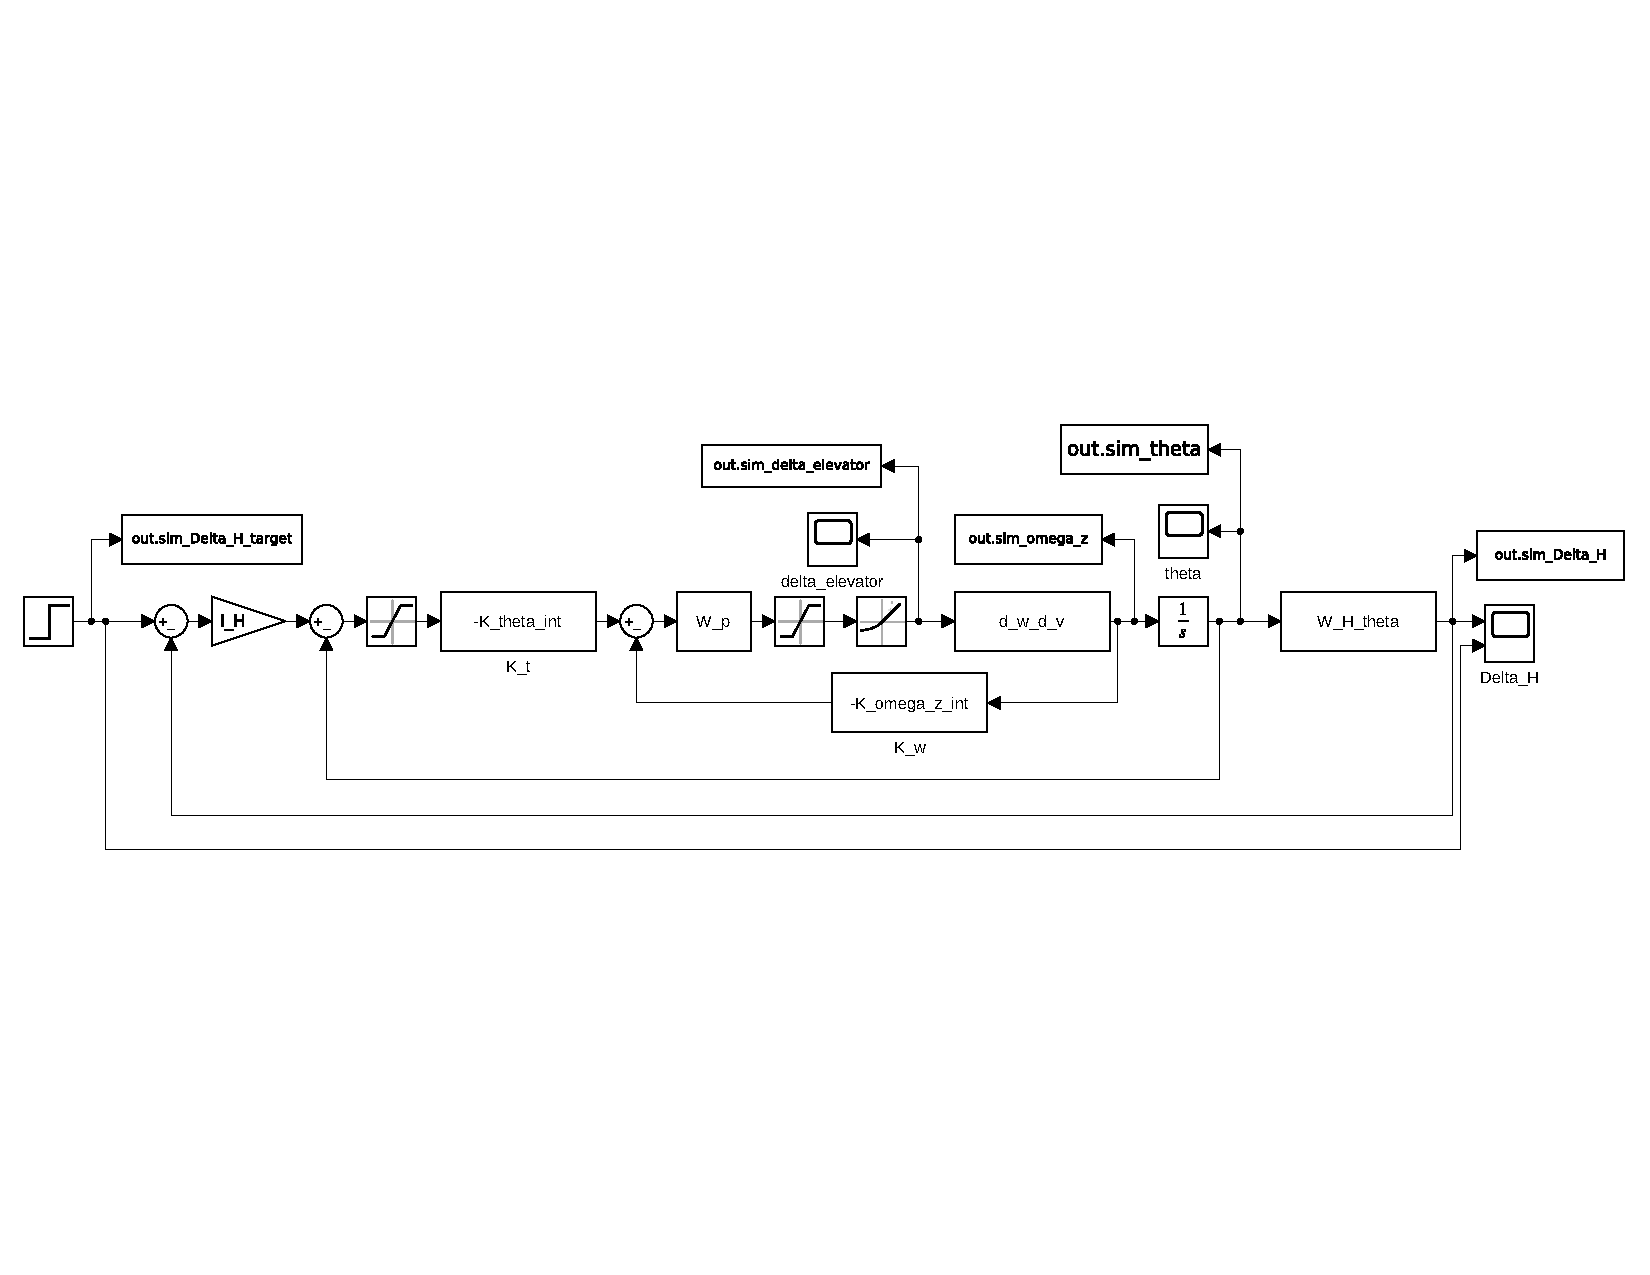
\includegraphics[clip, trim=0.4cm 6cm 0.4cm 7cm , width=1.00\textwidth]{./figures/model.pdf}
    \caption{Схема нелинейной модели}
    \label{fig:nonlinear_model_simulink}
\end{figure}

\subsection{Сравнение для разных максимальных скоростей отклонения руля высоты}

Графики изменения $\Delta H$, $\delta_{в}$, $\omega_z$, $\vartheta$ для
$\dot{\delta}_\text{в max} = 15\, \frac{\text{град.}}{\text{сек.}},\ 60\, \frac{\text{град.}}{\text{сек.}}$
представлены на рисунках \ref{fig:model_DD_Delta_H},
\ref{fig:model_DD_delta_elevator}, \ref{fig:model_DD_omega_z}, \ref{fig:model_DD_theta}.

\begin{figure}[H]
    \begin{minipage}{0.48\textwidth}
    \centering
    \resizebox{1.1\linewidth}{!}{%% Creator: Matplotlib, PGF backend
%%
%% To include the figure in your LaTeX document, write
%%   \input{<filename>.pgf}
%%
%% Make sure the required packages are loaded in your preamble
%%   \usepackage{pgf}
%%
%% Figures using additional raster images can only be included by \input if
%% they are in the same directory as the main LaTeX file. For loading figures
%% from other directories you can use the `import` package
%%   \usepackage{import}
%%
%% and then include the figures with
%%   \import{<path to file>}{<filename>.pgf}
%%
%% Matplotlib used the following preamble
%%   \usepackage[warn]{mathtext}
%%   \usepackage[T2A]{fontenc}
%%   \usepackage[utf8]{inputenc}
%%   \usepackage[english,russian]{babel}
%%
\begingroup%
\makeatletter%
\begin{pgfpicture}%
\pgfpathrectangle{\pgfpointorigin}{\pgfqpoint{6.400000in}{4.800000in}}%
\pgfusepath{use as bounding box, clip}%
\begin{pgfscope}%
\pgfsetbuttcap%
\pgfsetmiterjoin%
\definecolor{currentfill}{rgb}{1.000000,1.000000,1.000000}%
\pgfsetfillcolor{currentfill}%
\pgfsetlinewidth{0.000000pt}%
\definecolor{currentstroke}{rgb}{1.000000,1.000000,1.000000}%
\pgfsetstrokecolor{currentstroke}%
\pgfsetdash{}{0pt}%
\pgfpathmoveto{\pgfqpoint{0.000000in}{0.000000in}}%
\pgfpathlineto{\pgfqpoint{6.400000in}{0.000000in}}%
\pgfpathlineto{\pgfqpoint{6.400000in}{4.800000in}}%
\pgfpathlineto{\pgfqpoint{0.000000in}{4.800000in}}%
\pgfpathclose%
\pgfusepath{fill}%
\end{pgfscope}%
\begin{pgfscope}%
\pgfsetbuttcap%
\pgfsetmiterjoin%
\definecolor{currentfill}{rgb}{1.000000,1.000000,1.000000}%
\pgfsetfillcolor{currentfill}%
\pgfsetlinewidth{0.000000pt}%
\definecolor{currentstroke}{rgb}{0.000000,0.000000,0.000000}%
\pgfsetstrokecolor{currentstroke}%
\pgfsetstrokeopacity{0.000000}%
\pgfsetdash{}{0pt}%
\pgfpathmoveto{\pgfqpoint{0.800000in}{0.528000in}}%
\pgfpathlineto{\pgfqpoint{5.760000in}{0.528000in}}%
\pgfpathlineto{\pgfqpoint{5.760000in}{4.224000in}}%
\pgfpathlineto{\pgfqpoint{0.800000in}{4.224000in}}%
\pgfpathclose%
\pgfusepath{fill}%
\end{pgfscope}%
\begin{pgfscope}%
\pgfpathrectangle{\pgfqpoint{0.800000in}{0.528000in}}{\pgfqpoint{4.960000in}{3.696000in}}%
\pgfusepath{clip}%
\pgfsetrectcap%
\pgfsetroundjoin%
\pgfsetlinewidth{0.803000pt}%
\definecolor{currentstroke}{rgb}{0.690196,0.690196,0.690196}%
\pgfsetstrokecolor{currentstroke}%
\pgfsetdash{}{0pt}%
\pgfpathmoveto{\pgfqpoint{1.025455in}{0.528000in}}%
\pgfpathlineto{\pgfqpoint{1.025455in}{4.224000in}}%
\pgfusepath{stroke}%
\end{pgfscope}%
\begin{pgfscope}%
\pgfsetbuttcap%
\pgfsetroundjoin%
\definecolor{currentfill}{rgb}{0.000000,0.000000,0.000000}%
\pgfsetfillcolor{currentfill}%
\pgfsetlinewidth{0.803000pt}%
\definecolor{currentstroke}{rgb}{0.000000,0.000000,0.000000}%
\pgfsetstrokecolor{currentstroke}%
\pgfsetdash{}{0pt}%
\pgfsys@defobject{currentmarker}{\pgfqpoint{0.000000in}{-0.048611in}}{\pgfqpoint{0.000000in}{0.000000in}}{%
\pgfpathmoveto{\pgfqpoint{0.000000in}{0.000000in}}%
\pgfpathlineto{\pgfqpoint{0.000000in}{-0.048611in}}%
\pgfusepath{stroke,fill}%
}%
\begin{pgfscope}%
\pgfsys@transformshift{1.025455in}{0.528000in}%
\pgfsys@useobject{currentmarker}{}%
\end{pgfscope}%
\end{pgfscope}%
\begin{pgfscope}%
\definecolor{textcolor}{rgb}{0.000000,0.000000,0.000000}%
\pgfsetstrokecolor{textcolor}%
\pgfsetfillcolor{textcolor}%
\pgftext[x=1.025455in,y=0.430778in,,top]{\color{textcolor}\rmfamily\fontsize{10.000000}{12.000000}\selectfont \(\displaystyle {0}\)}%
\end{pgfscope}%
\begin{pgfscope}%
\pgfpathrectangle{\pgfqpoint{0.800000in}{0.528000in}}{\pgfqpoint{4.960000in}{3.696000in}}%
\pgfusepath{clip}%
\pgfsetrectcap%
\pgfsetroundjoin%
\pgfsetlinewidth{0.803000pt}%
\definecolor{currentstroke}{rgb}{0.690196,0.690196,0.690196}%
\pgfsetstrokecolor{currentstroke}%
\pgfsetdash{}{0pt}%
\pgfpathmoveto{\pgfqpoint{1.776970in}{0.528000in}}%
\pgfpathlineto{\pgfqpoint{1.776970in}{4.224000in}}%
\pgfusepath{stroke}%
\end{pgfscope}%
\begin{pgfscope}%
\pgfsetbuttcap%
\pgfsetroundjoin%
\definecolor{currentfill}{rgb}{0.000000,0.000000,0.000000}%
\pgfsetfillcolor{currentfill}%
\pgfsetlinewidth{0.803000pt}%
\definecolor{currentstroke}{rgb}{0.000000,0.000000,0.000000}%
\pgfsetstrokecolor{currentstroke}%
\pgfsetdash{}{0pt}%
\pgfsys@defobject{currentmarker}{\pgfqpoint{0.000000in}{-0.048611in}}{\pgfqpoint{0.000000in}{0.000000in}}{%
\pgfpathmoveto{\pgfqpoint{0.000000in}{0.000000in}}%
\pgfpathlineto{\pgfqpoint{0.000000in}{-0.048611in}}%
\pgfusepath{stroke,fill}%
}%
\begin{pgfscope}%
\pgfsys@transformshift{1.776970in}{0.528000in}%
\pgfsys@useobject{currentmarker}{}%
\end{pgfscope}%
\end{pgfscope}%
\begin{pgfscope}%
\definecolor{textcolor}{rgb}{0.000000,0.000000,0.000000}%
\pgfsetstrokecolor{textcolor}%
\pgfsetfillcolor{textcolor}%
\pgftext[x=1.776970in,y=0.430778in,,top]{\color{textcolor}\rmfamily\fontsize{10.000000}{12.000000}\selectfont \(\displaystyle {5}\)}%
\end{pgfscope}%
\begin{pgfscope}%
\pgfpathrectangle{\pgfqpoint{0.800000in}{0.528000in}}{\pgfqpoint{4.960000in}{3.696000in}}%
\pgfusepath{clip}%
\pgfsetrectcap%
\pgfsetroundjoin%
\pgfsetlinewidth{0.803000pt}%
\definecolor{currentstroke}{rgb}{0.690196,0.690196,0.690196}%
\pgfsetstrokecolor{currentstroke}%
\pgfsetdash{}{0pt}%
\pgfpathmoveto{\pgfqpoint{2.528485in}{0.528000in}}%
\pgfpathlineto{\pgfqpoint{2.528485in}{4.224000in}}%
\pgfusepath{stroke}%
\end{pgfscope}%
\begin{pgfscope}%
\pgfsetbuttcap%
\pgfsetroundjoin%
\definecolor{currentfill}{rgb}{0.000000,0.000000,0.000000}%
\pgfsetfillcolor{currentfill}%
\pgfsetlinewidth{0.803000pt}%
\definecolor{currentstroke}{rgb}{0.000000,0.000000,0.000000}%
\pgfsetstrokecolor{currentstroke}%
\pgfsetdash{}{0pt}%
\pgfsys@defobject{currentmarker}{\pgfqpoint{0.000000in}{-0.048611in}}{\pgfqpoint{0.000000in}{0.000000in}}{%
\pgfpathmoveto{\pgfqpoint{0.000000in}{0.000000in}}%
\pgfpathlineto{\pgfqpoint{0.000000in}{-0.048611in}}%
\pgfusepath{stroke,fill}%
}%
\begin{pgfscope}%
\pgfsys@transformshift{2.528485in}{0.528000in}%
\pgfsys@useobject{currentmarker}{}%
\end{pgfscope}%
\end{pgfscope}%
\begin{pgfscope}%
\definecolor{textcolor}{rgb}{0.000000,0.000000,0.000000}%
\pgfsetstrokecolor{textcolor}%
\pgfsetfillcolor{textcolor}%
\pgftext[x=2.528485in,y=0.430778in,,top]{\color{textcolor}\rmfamily\fontsize{10.000000}{12.000000}\selectfont \(\displaystyle {10}\)}%
\end{pgfscope}%
\begin{pgfscope}%
\pgfpathrectangle{\pgfqpoint{0.800000in}{0.528000in}}{\pgfqpoint{4.960000in}{3.696000in}}%
\pgfusepath{clip}%
\pgfsetrectcap%
\pgfsetroundjoin%
\pgfsetlinewidth{0.803000pt}%
\definecolor{currentstroke}{rgb}{0.690196,0.690196,0.690196}%
\pgfsetstrokecolor{currentstroke}%
\pgfsetdash{}{0pt}%
\pgfpathmoveto{\pgfqpoint{3.280000in}{0.528000in}}%
\pgfpathlineto{\pgfqpoint{3.280000in}{4.224000in}}%
\pgfusepath{stroke}%
\end{pgfscope}%
\begin{pgfscope}%
\pgfsetbuttcap%
\pgfsetroundjoin%
\definecolor{currentfill}{rgb}{0.000000,0.000000,0.000000}%
\pgfsetfillcolor{currentfill}%
\pgfsetlinewidth{0.803000pt}%
\definecolor{currentstroke}{rgb}{0.000000,0.000000,0.000000}%
\pgfsetstrokecolor{currentstroke}%
\pgfsetdash{}{0pt}%
\pgfsys@defobject{currentmarker}{\pgfqpoint{0.000000in}{-0.048611in}}{\pgfqpoint{0.000000in}{0.000000in}}{%
\pgfpathmoveto{\pgfqpoint{0.000000in}{0.000000in}}%
\pgfpathlineto{\pgfqpoint{0.000000in}{-0.048611in}}%
\pgfusepath{stroke,fill}%
}%
\begin{pgfscope}%
\pgfsys@transformshift{3.280000in}{0.528000in}%
\pgfsys@useobject{currentmarker}{}%
\end{pgfscope}%
\end{pgfscope}%
\begin{pgfscope}%
\definecolor{textcolor}{rgb}{0.000000,0.000000,0.000000}%
\pgfsetstrokecolor{textcolor}%
\pgfsetfillcolor{textcolor}%
\pgftext[x=3.280000in,y=0.430778in,,top]{\color{textcolor}\rmfamily\fontsize{10.000000}{12.000000}\selectfont \(\displaystyle {15}\)}%
\end{pgfscope}%
\begin{pgfscope}%
\pgfpathrectangle{\pgfqpoint{0.800000in}{0.528000in}}{\pgfqpoint{4.960000in}{3.696000in}}%
\pgfusepath{clip}%
\pgfsetrectcap%
\pgfsetroundjoin%
\pgfsetlinewidth{0.803000pt}%
\definecolor{currentstroke}{rgb}{0.690196,0.690196,0.690196}%
\pgfsetstrokecolor{currentstroke}%
\pgfsetdash{}{0pt}%
\pgfpathmoveto{\pgfqpoint{4.031515in}{0.528000in}}%
\pgfpathlineto{\pgfqpoint{4.031515in}{4.224000in}}%
\pgfusepath{stroke}%
\end{pgfscope}%
\begin{pgfscope}%
\pgfsetbuttcap%
\pgfsetroundjoin%
\definecolor{currentfill}{rgb}{0.000000,0.000000,0.000000}%
\pgfsetfillcolor{currentfill}%
\pgfsetlinewidth{0.803000pt}%
\definecolor{currentstroke}{rgb}{0.000000,0.000000,0.000000}%
\pgfsetstrokecolor{currentstroke}%
\pgfsetdash{}{0pt}%
\pgfsys@defobject{currentmarker}{\pgfqpoint{0.000000in}{-0.048611in}}{\pgfqpoint{0.000000in}{0.000000in}}{%
\pgfpathmoveto{\pgfqpoint{0.000000in}{0.000000in}}%
\pgfpathlineto{\pgfqpoint{0.000000in}{-0.048611in}}%
\pgfusepath{stroke,fill}%
}%
\begin{pgfscope}%
\pgfsys@transformshift{4.031515in}{0.528000in}%
\pgfsys@useobject{currentmarker}{}%
\end{pgfscope}%
\end{pgfscope}%
\begin{pgfscope}%
\definecolor{textcolor}{rgb}{0.000000,0.000000,0.000000}%
\pgfsetstrokecolor{textcolor}%
\pgfsetfillcolor{textcolor}%
\pgftext[x=4.031515in,y=0.430778in,,top]{\color{textcolor}\rmfamily\fontsize{10.000000}{12.000000}\selectfont \(\displaystyle {20}\)}%
\end{pgfscope}%
\begin{pgfscope}%
\pgfpathrectangle{\pgfqpoint{0.800000in}{0.528000in}}{\pgfqpoint{4.960000in}{3.696000in}}%
\pgfusepath{clip}%
\pgfsetrectcap%
\pgfsetroundjoin%
\pgfsetlinewidth{0.803000pt}%
\definecolor{currentstroke}{rgb}{0.690196,0.690196,0.690196}%
\pgfsetstrokecolor{currentstroke}%
\pgfsetdash{}{0pt}%
\pgfpathmoveto{\pgfqpoint{4.783030in}{0.528000in}}%
\pgfpathlineto{\pgfqpoint{4.783030in}{4.224000in}}%
\pgfusepath{stroke}%
\end{pgfscope}%
\begin{pgfscope}%
\pgfsetbuttcap%
\pgfsetroundjoin%
\definecolor{currentfill}{rgb}{0.000000,0.000000,0.000000}%
\pgfsetfillcolor{currentfill}%
\pgfsetlinewidth{0.803000pt}%
\definecolor{currentstroke}{rgb}{0.000000,0.000000,0.000000}%
\pgfsetstrokecolor{currentstroke}%
\pgfsetdash{}{0pt}%
\pgfsys@defobject{currentmarker}{\pgfqpoint{0.000000in}{-0.048611in}}{\pgfqpoint{0.000000in}{0.000000in}}{%
\pgfpathmoveto{\pgfqpoint{0.000000in}{0.000000in}}%
\pgfpathlineto{\pgfqpoint{0.000000in}{-0.048611in}}%
\pgfusepath{stroke,fill}%
}%
\begin{pgfscope}%
\pgfsys@transformshift{4.783030in}{0.528000in}%
\pgfsys@useobject{currentmarker}{}%
\end{pgfscope}%
\end{pgfscope}%
\begin{pgfscope}%
\definecolor{textcolor}{rgb}{0.000000,0.000000,0.000000}%
\pgfsetstrokecolor{textcolor}%
\pgfsetfillcolor{textcolor}%
\pgftext[x=4.783030in,y=0.430778in,,top]{\color{textcolor}\rmfamily\fontsize{10.000000}{12.000000}\selectfont \(\displaystyle {25}\)}%
\end{pgfscope}%
\begin{pgfscope}%
\pgfpathrectangle{\pgfqpoint{0.800000in}{0.528000in}}{\pgfqpoint{4.960000in}{3.696000in}}%
\pgfusepath{clip}%
\pgfsetrectcap%
\pgfsetroundjoin%
\pgfsetlinewidth{0.803000pt}%
\definecolor{currentstroke}{rgb}{0.690196,0.690196,0.690196}%
\pgfsetstrokecolor{currentstroke}%
\pgfsetdash{}{0pt}%
\pgfpathmoveto{\pgfqpoint{5.534545in}{0.528000in}}%
\pgfpathlineto{\pgfqpoint{5.534545in}{4.224000in}}%
\pgfusepath{stroke}%
\end{pgfscope}%
\begin{pgfscope}%
\pgfsetbuttcap%
\pgfsetroundjoin%
\definecolor{currentfill}{rgb}{0.000000,0.000000,0.000000}%
\pgfsetfillcolor{currentfill}%
\pgfsetlinewidth{0.803000pt}%
\definecolor{currentstroke}{rgb}{0.000000,0.000000,0.000000}%
\pgfsetstrokecolor{currentstroke}%
\pgfsetdash{}{0pt}%
\pgfsys@defobject{currentmarker}{\pgfqpoint{0.000000in}{-0.048611in}}{\pgfqpoint{0.000000in}{0.000000in}}{%
\pgfpathmoveto{\pgfqpoint{0.000000in}{0.000000in}}%
\pgfpathlineto{\pgfqpoint{0.000000in}{-0.048611in}}%
\pgfusepath{stroke,fill}%
}%
\begin{pgfscope}%
\pgfsys@transformshift{5.534545in}{0.528000in}%
\pgfsys@useobject{currentmarker}{}%
\end{pgfscope}%
\end{pgfscope}%
\begin{pgfscope}%
\definecolor{textcolor}{rgb}{0.000000,0.000000,0.000000}%
\pgfsetstrokecolor{textcolor}%
\pgfsetfillcolor{textcolor}%
\pgftext[x=5.534545in,y=0.430778in,,top]{\color{textcolor}\rmfamily\fontsize{10.000000}{12.000000}\selectfont \(\displaystyle {30}\)}%
\end{pgfscope}%
\begin{pgfscope}%
\definecolor{textcolor}{rgb}{0.000000,0.000000,0.000000}%
\pgfsetstrokecolor{textcolor}%
\pgfsetfillcolor{textcolor}%
\pgftext[x=3.280000in,y=0.251796in,,top]{\color{textcolor}\rmfamily\fontsize{10.000000}{12.000000}\selectfont \(\displaystyle t,\ с\)}%
\end{pgfscope}%
\begin{pgfscope}%
\pgfpathrectangle{\pgfqpoint{0.800000in}{0.528000in}}{\pgfqpoint{4.960000in}{3.696000in}}%
\pgfusepath{clip}%
\pgfsetrectcap%
\pgfsetroundjoin%
\pgfsetlinewidth{0.803000pt}%
\definecolor{currentstroke}{rgb}{0.690196,0.690196,0.690196}%
\pgfsetstrokecolor{currentstroke}%
\pgfsetdash{}{0pt}%
\pgfpathmoveto{\pgfqpoint{0.800000in}{0.696000in}}%
\pgfpathlineto{\pgfqpoint{5.760000in}{0.696000in}}%
\pgfusepath{stroke}%
\end{pgfscope}%
\begin{pgfscope}%
\pgfsetbuttcap%
\pgfsetroundjoin%
\definecolor{currentfill}{rgb}{0.000000,0.000000,0.000000}%
\pgfsetfillcolor{currentfill}%
\pgfsetlinewidth{0.803000pt}%
\definecolor{currentstroke}{rgb}{0.000000,0.000000,0.000000}%
\pgfsetstrokecolor{currentstroke}%
\pgfsetdash{}{0pt}%
\pgfsys@defobject{currentmarker}{\pgfqpoint{-0.048611in}{0.000000in}}{\pgfqpoint{-0.000000in}{0.000000in}}{%
\pgfpathmoveto{\pgfqpoint{-0.000000in}{0.000000in}}%
\pgfpathlineto{\pgfqpoint{-0.048611in}{0.000000in}}%
\pgfusepath{stroke,fill}%
}%
\begin{pgfscope}%
\pgfsys@transformshift{0.800000in}{0.696000in}%
\pgfsys@useobject{currentmarker}{}%
\end{pgfscope}%
\end{pgfscope}%
\begin{pgfscope}%
\definecolor{textcolor}{rgb}{0.000000,0.000000,0.000000}%
\pgfsetstrokecolor{textcolor}%
\pgfsetfillcolor{textcolor}%
\pgftext[x=0.633333in, y=0.647786in, left, base]{\color{textcolor}\rmfamily\fontsize{10.000000}{12.000000}\selectfont \(\displaystyle {0}\)}%
\end{pgfscope}%
\begin{pgfscope}%
\pgfpathrectangle{\pgfqpoint{0.800000in}{0.528000in}}{\pgfqpoint{4.960000in}{3.696000in}}%
\pgfusepath{clip}%
\pgfsetrectcap%
\pgfsetroundjoin%
\pgfsetlinewidth{0.803000pt}%
\definecolor{currentstroke}{rgb}{0.690196,0.690196,0.690196}%
\pgfsetstrokecolor{currentstroke}%
\pgfsetdash{}{0pt}%
\pgfpathmoveto{\pgfqpoint{0.800000in}{1.238387in}}%
\pgfpathlineto{\pgfqpoint{5.760000in}{1.238387in}}%
\pgfusepath{stroke}%
\end{pgfscope}%
\begin{pgfscope}%
\pgfsetbuttcap%
\pgfsetroundjoin%
\definecolor{currentfill}{rgb}{0.000000,0.000000,0.000000}%
\pgfsetfillcolor{currentfill}%
\pgfsetlinewidth{0.803000pt}%
\definecolor{currentstroke}{rgb}{0.000000,0.000000,0.000000}%
\pgfsetstrokecolor{currentstroke}%
\pgfsetdash{}{0pt}%
\pgfsys@defobject{currentmarker}{\pgfqpoint{-0.048611in}{0.000000in}}{\pgfqpoint{-0.000000in}{0.000000in}}{%
\pgfpathmoveto{\pgfqpoint{-0.000000in}{0.000000in}}%
\pgfpathlineto{\pgfqpoint{-0.048611in}{0.000000in}}%
\pgfusepath{stroke,fill}%
}%
\begin{pgfscope}%
\pgfsys@transformshift{0.800000in}{1.238387in}%
\pgfsys@useobject{currentmarker}{}%
\end{pgfscope}%
\end{pgfscope}%
\begin{pgfscope}%
\definecolor{textcolor}{rgb}{0.000000,0.000000,0.000000}%
\pgfsetstrokecolor{textcolor}%
\pgfsetfillcolor{textcolor}%
\pgftext[x=0.563888in, y=1.190174in, left, base]{\color{textcolor}\rmfamily\fontsize{10.000000}{12.000000}\selectfont \(\displaystyle {20}\)}%
\end{pgfscope}%
\begin{pgfscope}%
\pgfpathrectangle{\pgfqpoint{0.800000in}{0.528000in}}{\pgfqpoint{4.960000in}{3.696000in}}%
\pgfusepath{clip}%
\pgfsetrectcap%
\pgfsetroundjoin%
\pgfsetlinewidth{0.803000pt}%
\definecolor{currentstroke}{rgb}{0.690196,0.690196,0.690196}%
\pgfsetstrokecolor{currentstroke}%
\pgfsetdash{}{0pt}%
\pgfpathmoveto{\pgfqpoint{0.800000in}{1.780775in}}%
\pgfpathlineto{\pgfqpoint{5.760000in}{1.780775in}}%
\pgfusepath{stroke}%
\end{pgfscope}%
\begin{pgfscope}%
\pgfsetbuttcap%
\pgfsetroundjoin%
\definecolor{currentfill}{rgb}{0.000000,0.000000,0.000000}%
\pgfsetfillcolor{currentfill}%
\pgfsetlinewidth{0.803000pt}%
\definecolor{currentstroke}{rgb}{0.000000,0.000000,0.000000}%
\pgfsetstrokecolor{currentstroke}%
\pgfsetdash{}{0pt}%
\pgfsys@defobject{currentmarker}{\pgfqpoint{-0.048611in}{0.000000in}}{\pgfqpoint{-0.000000in}{0.000000in}}{%
\pgfpathmoveto{\pgfqpoint{-0.000000in}{0.000000in}}%
\pgfpathlineto{\pgfqpoint{-0.048611in}{0.000000in}}%
\pgfusepath{stroke,fill}%
}%
\begin{pgfscope}%
\pgfsys@transformshift{0.800000in}{1.780775in}%
\pgfsys@useobject{currentmarker}{}%
\end{pgfscope}%
\end{pgfscope}%
\begin{pgfscope}%
\definecolor{textcolor}{rgb}{0.000000,0.000000,0.000000}%
\pgfsetstrokecolor{textcolor}%
\pgfsetfillcolor{textcolor}%
\pgftext[x=0.563888in, y=1.732561in, left, base]{\color{textcolor}\rmfamily\fontsize{10.000000}{12.000000}\selectfont \(\displaystyle {40}\)}%
\end{pgfscope}%
\begin{pgfscope}%
\pgfpathrectangle{\pgfqpoint{0.800000in}{0.528000in}}{\pgfqpoint{4.960000in}{3.696000in}}%
\pgfusepath{clip}%
\pgfsetrectcap%
\pgfsetroundjoin%
\pgfsetlinewidth{0.803000pt}%
\definecolor{currentstroke}{rgb}{0.690196,0.690196,0.690196}%
\pgfsetstrokecolor{currentstroke}%
\pgfsetdash{}{0pt}%
\pgfpathmoveto{\pgfqpoint{0.800000in}{2.323162in}}%
\pgfpathlineto{\pgfqpoint{5.760000in}{2.323162in}}%
\pgfusepath{stroke}%
\end{pgfscope}%
\begin{pgfscope}%
\pgfsetbuttcap%
\pgfsetroundjoin%
\definecolor{currentfill}{rgb}{0.000000,0.000000,0.000000}%
\pgfsetfillcolor{currentfill}%
\pgfsetlinewidth{0.803000pt}%
\definecolor{currentstroke}{rgb}{0.000000,0.000000,0.000000}%
\pgfsetstrokecolor{currentstroke}%
\pgfsetdash{}{0pt}%
\pgfsys@defobject{currentmarker}{\pgfqpoint{-0.048611in}{0.000000in}}{\pgfqpoint{-0.000000in}{0.000000in}}{%
\pgfpathmoveto{\pgfqpoint{-0.000000in}{0.000000in}}%
\pgfpathlineto{\pgfqpoint{-0.048611in}{0.000000in}}%
\pgfusepath{stroke,fill}%
}%
\begin{pgfscope}%
\pgfsys@transformshift{0.800000in}{2.323162in}%
\pgfsys@useobject{currentmarker}{}%
\end{pgfscope}%
\end{pgfscope}%
\begin{pgfscope}%
\definecolor{textcolor}{rgb}{0.000000,0.000000,0.000000}%
\pgfsetstrokecolor{textcolor}%
\pgfsetfillcolor{textcolor}%
\pgftext[x=0.563888in, y=2.274948in, left, base]{\color{textcolor}\rmfamily\fontsize{10.000000}{12.000000}\selectfont \(\displaystyle {60}\)}%
\end{pgfscope}%
\begin{pgfscope}%
\pgfpathrectangle{\pgfqpoint{0.800000in}{0.528000in}}{\pgfqpoint{4.960000in}{3.696000in}}%
\pgfusepath{clip}%
\pgfsetrectcap%
\pgfsetroundjoin%
\pgfsetlinewidth{0.803000pt}%
\definecolor{currentstroke}{rgb}{0.690196,0.690196,0.690196}%
\pgfsetstrokecolor{currentstroke}%
\pgfsetdash{}{0pt}%
\pgfpathmoveto{\pgfqpoint{0.800000in}{2.865549in}}%
\pgfpathlineto{\pgfqpoint{5.760000in}{2.865549in}}%
\pgfusepath{stroke}%
\end{pgfscope}%
\begin{pgfscope}%
\pgfsetbuttcap%
\pgfsetroundjoin%
\definecolor{currentfill}{rgb}{0.000000,0.000000,0.000000}%
\pgfsetfillcolor{currentfill}%
\pgfsetlinewidth{0.803000pt}%
\definecolor{currentstroke}{rgb}{0.000000,0.000000,0.000000}%
\pgfsetstrokecolor{currentstroke}%
\pgfsetdash{}{0pt}%
\pgfsys@defobject{currentmarker}{\pgfqpoint{-0.048611in}{0.000000in}}{\pgfqpoint{-0.000000in}{0.000000in}}{%
\pgfpathmoveto{\pgfqpoint{-0.000000in}{0.000000in}}%
\pgfpathlineto{\pgfqpoint{-0.048611in}{0.000000in}}%
\pgfusepath{stroke,fill}%
}%
\begin{pgfscope}%
\pgfsys@transformshift{0.800000in}{2.865549in}%
\pgfsys@useobject{currentmarker}{}%
\end{pgfscope}%
\end{pgfscope}%
\begin{pgfscope}%
\definecolor{textcolor}{rgb}{0.000000,0.000000,0.000000}%
\pgfsetstrokecolor{textcolor}%
\pgfsetfillcolor{textcolor}%
\pgftext[x=0.563888in, y=2.817336in, left, base]{\color{textcolor}\rmfamily\fontsize{10.000000}{12.000000}\selectfont \(\displaystyle {80}\)}%
\end{pgfscope}%
\begin{pgfscope}%
\pgfpathrectangle{\pgfqpoint{0.800000in}{0.528000in}}{\pgfqpoint{4.960000in}{3.696000in}}%
\pgfusepath{clip}%
\pgfsetrectcap%
\pgfsetroundjoin%
\pgfsetlinewidth{0.803000pt}%
\definecolor{currentstroke}{rgb}{0.690196,0.690196,0.690196}%
\pgfsetstrokecolor{currentstroke}%
\pgfsetdash{}{0pt}%
\pgfpathmoveto{\pgfqpoint{0.800000in}{3.407936in}}%
\pgfpathlineto{\pgfqpoint{5.760000in}{3.407936in}}%
\pgfusepath{stroke}%
\end{pgfscope}%
\begin{pgfscope}%
\pgfsetbuttcap%
\pgfsetroundjoin%
\definecolor{currentfill}{rgb}{0.000000,0.000000,0.000000}%
\pgfsetfillcolor{currentfill}%
\pgfsetlinewidth{0.803000pt}%
\definecolor{currentstroke}{rgb}{0.000000,0.000000,0.000000}%
\pgfsetstrokecolor{currentstroke}%
\pgfsetdash{}{0pt}%
\pgfsys@defobject{currentmarker}{\pgfqpoint{-0.048611in}{0.000000in}}{\pgfqpoint{-0.000000in}{0.000000in}}{%
\pgfpathmoveto{\pgfqpoint{-0.000000in}{0.000000in}}%
\pgfpathlineto{\pgfqpoint{-0.048611in}{0.000000in}}%
\pgfusepath{stroke,fill}%
}%
\begin{pgfscope}%
\pgfsys@transformshift{0.800000in}{3.407936in}%
\pgfsys@useobject{currentmarker}{}%
\end{pgfscope}%
\end{pgfscope}%
\begin{pgfscope}%
\definecolor{textcolor}{rgb}{0.000000,0.000000,0.000000}%
\pgfsetstrokecolor{textcolor}%
\pgfsetfillcolor{textcolor}%
\pgftext[x=0.494444in, y=3.359723in, left, base]{\color{textcolor}\rmfamily\fontsize{10.000000}{12.000000}\selectfont \(\displaystyle {100}\)}%
\end{pgfscope}%
\begin{pgfscope}%
\pgfpathrectangle{\pgfqpoint{0.800000in}{0.528000in}}{\pgfqpoint{4.960000in}{3.696000in}}%
\pgfusepath{clip}%
\pgfsetrectcap%
\pgfsetroundjoin%
\pgfsetlinewidth{0.803000pt}%
\definecolor{currentstroke}{rgb}{0.690196,0.690196,0.690196}%
\pgfsetstrokecolor{currentstroke}%
\pgfsetdash{}{0pt}%
\pgfpathmoveto{\pgfqpoint{0.800000in}{3.950324in}}%
\pgfpathlineto{\pgfqpoint{5.760000in}{3.950324in}}%
\pgfusepath{stroke}%
\end{pgfscope}%
\begin{pgfscope}%
\pgfsetbuttcap%
\pgfsetroundjoin%
\definecolor{currentfill}{rgb}{0.000000,0.000000,0.000000}%
\pgfsetfillcolor{currentfill}%
\pgfsetlinewidth{0.803000pt}%
\definecolor{currentstroke}{rgb}{0.000000,0.000000,0.000000}%
\pgfsetstrokecolor{currentstroke}%
\pgfsetdash{}{0pt}%
\pgfsys@defobject{currentmarker}{\pgfqpoint{-0.048611in}{0.000000in}}{\pgfqpoint{-0.000000in}{0.000000in}}{%
\pgfpathmoveto{\pgfqpoint{-0.000000in}{0.000000in}}%
\pgfpathlineto{\pgfqpoint{-0.048611in}{0.000000in}}%
\pgfusepath{stroke,fill}%
}%
\begin{pgfscope}%
\pgfsys@transformshift{0.800000in}{3.950324in}%
\pgfsys@useobject{currentmarker}{}%
\end{pgfscope}%
\end{pgfscope}%
\begin{pgfscope}%
\definecolor{textcolor}{rgb}{0.000000,0.000000,0.000000}%
\pgfsetstrokecolor{textcolor}%
\pgfsetfillcolor{textcolor}%
\pgftext[x=0.494444in, y=3.902110in, left, base]{\color{textcolor}\rmfamily\fontsize{10.000000}{12.000000}\selectfont \(\displaystyle {120}\)}%
\end{pgfscope}%
\begin{pgfscope}%
\definecolor{textcolor}{rgb}{0.000000,0.000000,0.000000}%
\pgfsetstrokecolor{textcolor}%
\pgfsetfillcolor{textcolor}%
\pgftext[x=0.438888in,y=2.376000in,,bottom,rotate=90.000000]{\color{textcolor}\rmfamily\fontsize{10.000000}{12.000000}\selectfont \(\displaystyle \Delta H,\ м\)}%
\end{pgfscope}%
\begin{pgfscope}%
\pgfpathrectangle{\pgfqpoint{0.800000in}{0.528000in}}{\pgfqpoint{4.960000in}{3.696000in}}%
\pgfusepath{clip}%
\pgfsetrectcap%
\pgfsetroundjoin%
\pgfsetlinewidth{1.505625pt}%
\definecolor{currentstroke}{rgb}{0.121569,0.466667,0.705882}%
\pgfsetstrokecolor{currentstroke}%
\pgfsetdash{}{0pt}%
\pgfpathmoveto{\pgfqpoint{1.025455in}{0.696000in}}%
\pgfpathlineto{\pgfqpoint{1.277362in}{0.697108in}}%
\pgfpathlineto{\pgfqpoint{1.307122in}{0.699799in}}%
\pgfpathlineto{\pgfqpoint{1.330720in}{0.704125in}}%
\pgfpathlineto{\pgfqpoint{1.351762in}{0.710230in}}%
\pgfpathlineto{\pgfqpoint{1.371602in}{0.718305in}}%
\pgfpathlineto{\pgfqpoint{1.391142in}{0.728686in}}%
\pgfpathlineto{\pgfqpoint{1.410982in}{0.741782in}}%
\pgfpathlineto{\pgfqpoint{1.431874in}{0.758295in}}%
\pgfpathlineto{\pgfqpoint{1.454269in}{0.778889in}}%
\pgfpathlineto{\pgfqpoint{1.478768in}{0.804502in}}%
\pgfpathlineto{\pgfqpoint{1.505673in}{0.835918in}}%
\pgfpathlineto{\pgfqpoint{1.534381in}{0.872912in}}%
\pgfpathlineto{\pgfqpoint{1.564291in}{0.915141in}}%
\pgfpathlineto{\pgfqpoint{1.595554in}{0.963201in}}%
\pgfpathlineto{\pgfqpoint{1.628470in}{1.017960in}}%
\pgfpathlineto{\pgfqpoint{1.663190in}{1.080105in}}%
\pgfpathlineto{\pgfqpoint{1.700015in}{1.150645in}}%
\pgfpathlineto{\pgfqpoint{1.739244in}{1.230679in}}%
\pgfpathlineto{\pgfqpoint{1.781178in}{1.321388in}}%
\pgfpathlineto{\pgfqpoint{1.825968in}{1.423667in}}%
\pgfpathlineto{\pgfqpoint{1.874065in}{1.539130in}}%
\pgfpathlineto{\pgfqpoint{1.925920in}{1.669496in}}%
\pgfpathlineto{\pgfqpoint{1.982133in}{1.816960in}}%
\pgfpathlineto{\pgfqpoint{2.043156in}{1.983412in}}%
\pgfpathlineto{\pgfqpoint{2.111695in}{2.177048in}}%
\pgfpathlineto{\pgfqpoint{2.212097in}{2.468303in}}%
\pgfpathlineto{\pgfqpoint{2.324674in}{2.793111in}}%
\pgfpathlineto{\pgfqpoint{2.388703in}{2.971002in}}%
\pgfpathlineto{\pgfqpoint{2.442512in}{3.114097in}}%
\pgfpathlineto{\pgfqpoint{2.490608in}{3.235815in}}%
\pgfpathlineto{\pgfqpoint{2.534798in}{3.341707in}}%
\pgfpathlineto{\pgfqpoint{2.575981in}{3.434742in}}%
\pgfpathlineto{\pgfqpoint{2.614909in}{3.517297in}}%
\pgfpathlineto{\pgfqpoint{2.651884in}{3.590596in}}%
\pgfpathlineto{\pgfqpoint{2.687205in}{3.655782in}}%
\pgfpathlineto{\pgfqpoint{2.721173in}{3.713886in}}%
\pgfpathlineto{\pgfqpoint{2.753939in}{3.765590in}}%
\pgfpathlineto{\pgfqpoint{2.785503in}{3.811312in}}%
\pgfpathlineto{\pgfqpoint{2.816165in}{3.851864in}}%
\pgfpathlineto{\pgfqpoint{2.845925in}{3.887575in}}%
\pgfpathlineto{\pgfqpoint{2.874783in}{3.918782in}}%
\pgfpathlineto{\pgfqpoint{2.902890in}{3.945959in}}%
\pgfpathlineto{\pgfqpoint{2.930395in}{3.969509in}}%
\pgfpathlineto{\pgfqpoint{2.957450in}{3.989775in}}%
\pgfpathlineto{\pgfqpoint{2.984053in}{4.006943in}}%
\pgfpathlineto{\pgfqpoint{3.010206in}{4.021202in}}%
\pgfpathlineto{\pgfqpoint{3.036208in}{4.032862in}}%
\pgfpathlineto{\pgfqpoint{3.062061in}{4.042025in}}%
\pgfpathlineto{\pgfqpoint{3.087913in}{4.048831in}}%
\pgfpathlineto{\pgfqpoint{3.113765in}{4.053347in}}%
\pgfpathlineto{\pgfqpoint{3.139918in}{4.055663in}}%
\pgfpathlineto{\pgfqpoint{3.166521in}{4.055777in}}%
\pgfpathlineto{\pgfqpoint{3.193576in}{4.053666in}}%
\pgfpathlineto{\pgfqpoint{3.221382in}{4.049257in}}%
\pgfpathlineto{\pgfqpoint{3.250090in}{4.042441in}}%
\pgfpathlineto{\pgfqpoint{3.280000in}{4.033026in}}%
\pgfpathlineto{\pgfqpoint{3.311263in}{4.020816in}}%
\pgfpathlineto{\pgfqpoint{3.344029in}{4.005601in}}%
\pgfpathlineto{\pgfqpoint{3.378749in}{3.986995in}}%
\pgfpathlineto{\pgfqpoint{3.415874in}{3.964537in}}%
\pgfpathlineto{\pgfqpoint{3.456005in}{3.937609in}}%
\pgfpathlineto{\pgfqpoint{3.499893in}{3.905428in}}%
\pgfpathlineto{\pgfqpoint{3.549193in}{3.866450in}}%
\pgfpathlineto{\pgfqpoint{3.606759in}{3.817992in}}%
\pgfpathlineto{\pgfqpoint{3.680558in}{3.752771in}}%
\pgfpathlineto{\pgfqpoint{3.918487in}{3.540315in}}%
\pgfpathlineto{\pgfqpoint{3.982366in}{3.487543in}}%
\pgfpathlineto{\pgfqpoint{4.039181in}{3.443436in}}%
\pgfpathlineto{\pgfqpoint{4.091787in}{3.405371in}}%
\pgfpathlineto{\pgfqpoint{4.141387in}{3.372186in}}%
\pgfpathlineto{\pgfqpoint{4.188882in}{3.343049in}}%
\pgfpathlineto{\pgfqpoint{4.234875in}{3.317416in}}%
\pgfpathlineto{\pgfqpoint{4.279665in}{3.294973in}}%
\pgfpathlineto{\pgfqpoint{4.323704in}{3.275377in}}%
\pgfpathlineto{\pgfqpoint{4.367142in}{3.258467in}}%
\pgfpathlineto{\pgfqpoint{4.410279in}{3.244044in}}%
\pgfpathlineto{\pgfqpoint{4.453416in}{3.231961in}}%
\pgfpathlineto{\pgfqpoint{4.496703in}{3.222143in}}%
\pgfpathlineto{\pgfqpoint{4.540441in}{3.214508in}}%
\pgfpathlineto{\pgfqpoint{4.584781in}{3.209030in}}%
\pgfpathlineto{\pgfqpoint{4.630022in}{3.205688in}}%
\pgfpathlineto{\pgfqpoint{4.676465in}{3.204493in}}%
\pgfpathlineto{\pgfqpoint{4.724562in}{3.205492in}}%
\pgfpathlineto{\pgfqpoint{4.774764in}{3.208780in}}%
\pgfpathlineto{\pgfqpoint{4.827670in}{3.214501in}}%
\pgfpathlineto{\pgfqpoint{4.884034in}{3.222861in}}%
\pgfpathlineto{\pgfqpoint{4.945207in}{3.234221in}}%
\pgfpathlineto{\pgfqpoint{5.013295in}{3.249178in}}%
\pgfpathlineto{\pgfqpoint{5.092655in}{3.268966in}}%
\pgfpathlineto{\pgfqpoint{5.195913in}{3.297165in}}%
\pgfpathlineto{\pgfqpoint{5.488102in}{3.378235in}}%
\pgfpathlineto{\pgfqpoint{5.534545in}{3.389858in}}%
\pgfpathlineto{\pgfqpoint{5.534545in}{3.389858in}}%
\pgfusepath{stroke}%
\end{pgfscope}%
\begin{pgfscope}%
\pgfpathrectangle{\pgfqpoint{0.800000in}{0.528000in}}{\pgfqpoint{4.960000in}{3.696000in}}%
\pgfusepath{clip}%
\pgfsetbuttcap%
\pgfsetroundjoin%
\pgfsetlinewidth{1.505625pt}%
\definecolor{currentstroke}{rgb}{1.000000,0.498039,0.054902}%
\pgfsetstrokecolor{currentstroke}%
\pgfsetdash{{9.600000pt}{2.400000pt}{1.500000pt}{2.400000pt}}{0.000000pt}%
\pgfpathmoveto{\pgfqpoint{1.025455in}{0.696000in}}%
\pgfpathlineto{\pgfqpoint{1.254516in}{0.697108in}}%
\pgfpathlineto{\pgfqpoint{1.282322in}{0.699968in}}%
\pgfpathlineto{\pgfqpoint{1.306672in}{0.704693in}}%
\pgfpathlineto{\pgfqpoint{1.329668in}{0.711417in}}%
\pgfpathlineto{\pgfqpoint{1.352063in}{0.720284in}}%
\pgfpathlineto{\pgfqpoint{1.374458in}{0.731568in}}%
\pgfpathlineto{\pgfqpoint{1.397004in}{0.745444in}}%
\pgfpathlineto{\pgfqpoint{1.420000in}{0.762234in}}%
\pgfpathlineto{\pgfqpoint{1.443748in}{0.782368in}}%
\pgfpathlineto{\pgfqpoint{1.468398in}{0.806239in}}%
\pgfpathlineto{\pgfqpoint{1.494099in}{0.834292in}}%
\pgfpathlineto{\pgfqpoint{1.521004in}{0.867021in}}%
\pgfpathlineto{\pgfqpoint{1.549261in}{0.904969in}}%
\pgfpathlineto{\pgfqpoint{1.579021in}{0.948728in}}%
\pgfpathlineto{\pgfqpoint{1.610434in}{0.998934in}}%
\pgfpathlineto{\pgfqpoint{1.643801in}{1.056528in}}%
\pgfpathlineto{\pgfqpoint{1.679273in}{1.122274in}}%
\pgfpathlineto{\pgfqpoint{1.716999in}{1.196959in}}%
\pgfpathlineto{\pgfqpoint{1.757430in}{1.282035in}}%
\pgfpathlineto{\pgfqpoint{1.800718in}{1.378416in}}%
\pgfpathlineto{\pgfqpoint{1.847161in}{1.487366in}}%
\pgfpathlineto{\pgfqpoint{1.897212in}{1.610569in}}%
\pgfpathlineto{\pgfqpoint{1.951171in}{1.749406in}}%
\pgfpathlineto{\pgfqpoint{2.009789in}{1.906486in}}%
\pgfpathlineto{\pgfqpoint{2.073968in}{2.084974in}}%
\pgfpathlineto{\pgfqpoint{2.152577in}{2.310601in}}%
\pgfpathlineto{\pgfqpoint{2.340155in}{2.851640in}}%
\pgfpathlineto{\pgfqpoint{2.400276in}{3.016566in}}%
\pgfpathlineto{\pgfqpoint{2.451981in}{3.152087in}}%
\pgfpathlineto{\pgfqpoint{2.498725in}{3.268512in}}%
\pgfpathlineto{\pgfqpoint{2.542012in}{3.370465in}}%
\pgfpathlineto{\pgfqpoint{2.582594in}{3.460445in}}%
\pgfpathlineto{\pgfqpoint{2.620921in}{3.540111in}}%
\pgfpathlineto{\pgfqpoint{2.657445in}{3.610985in}}%
\pgfpathlineto{\pgfqpoint{2.692315in}{3.673893in}}%
\pgfpathlineto{\pgfqpoint{2.725833in}{3.729867in}}%
\pgfpathlineto{\pgfqpoint{2.758148in}{3.779589in}}%
\pgfpathlineto{\pgfqpoint{2.789411in}{3.823685in}}%
\pgfpathlineto{\pgfqpoint{2.819772in}{3.862717in}}%
\pgfpathlineto{\pgfqpoint{2.849232in}{3.897018in}}%
\pgfpathlineto{\pgfqpoint{2.877939in}{3.927072in}}%
\pgfpathlineto{\pgfqpoint{2.905896in}{3.953164in}}%
\pgfpathlineto{\pgfqpoint{2.933251in}{3.975696in}}%
\pgfpathlineto{\pgfqpoint{2.960155in}{3.995002in}}%
\pgfpathlineto{\pgfqpoint{2.986608in}{4.011272in}}%
\pgfpathlineto{\pgfqpoint{3.012761in}{4.024764in}}%
\pgfpathlineto{\pgfqpoint{3.038613in}{4.035622in}}%
\pgfpathlineto{\pgfqpoint{3.064465in}{4.044078in}}%
\pgfpathlineto{\pgfqpoint{3.090318in}{4.050196in}}%
\pgfpathlineto{\pgfqpoint{3.116320in}{4.054064in}}%
\pgfpathlineto{\pgfqpoint{3.142623in}{4.055722in}}%
\pgfpathlineto{\pgfqpoint{3.169377in}{4.055168in}}%
\pgfpathlineto{\pgfqpoint{3.196732in}{4.052361in}}%
\pgfpathlineto{\pgfqpoint{3.224839in}{4.047223in}}%
\pgfpathlineto{\pgfqpoint{3.253847in}{4.039647in}}%
\pgfpathlineto{\pgfqpoint{3.284058in}{4.029438in}}%
\pgfpathlineto{\pgfqpoint{3.315772in}{4.016341in}}%
\pgfpathlineto{\pgfqpoint{3.349139in}{4.000118in}}%
\pgfpathlineto{\pgfqpoint{3.384611in}{3.980357in}}%
\pgfpathlineto{\pgfqpoint{3.422638in}{3.956575in}}%
\pgfpathlineto{\pgfqpoint{3.463821in}{3.928143in}}%
\pgfpathlineto{\pgfqpoint{3.509212in}{3.894041in}}%
\pgfpathlineto{\pgfqpoint{3.560616in}{3.852561in}}%
\pgfpathlineto{\pgfqpoint{3.621789in}{3.800221in}}%
\pgfpathlineto{\pgfqpoint{3.705358in}{3.725539in}}%
\pgfpathlineto{\pgfqpoint{3.881062in}{3.567904in}}%
\pgfpathlineto{\pgfqpoint{3.949901in}{3.509622in}}%
\pgfpathlineto{\pgfqpoint{4.009421in}{3.462090in}}%
\pgfpathlineto{\pgfqpoint{4.063680in}{3.421560in}}%
\pgfpathlineto{\pgfqpoint{4.114482in}{3.386347in}}%
\pgfpathlineto{\pgfqpoint{4.162880in}{3.355472in}}%
\pgfpathlineto{\pgfqpoint{4.209474in}{3.328356in}}%
\pgfpathlineto{\pgfqpoint{4.254865in}{3.304495in}}%
\pgfpathlineto{\pgfqpoint{4.299205in}{3.283681in}}%
\pgfpathlineto{\pgfqpoint{4.342943in}{3.265595in}}%
\pgfpathlineto{\pgfqpoint{4.386230in}{3.250092in}}%
\pgfpathlineto{\pgfqpoint{4.429367in}{3.236998in}}%
\pgfpathlineto{\pgfqpoint{4.472504in}{3.226219in}}%
\pgfpathlineto{\pgfqpoint{4.515942in}{3.217651in}}%
\pgfpathlineto{\pgfqpoint{4.559981in}{3.211234in}}%
\pgfpathlineto{\pgfqpoint{4.604771in}{3.206957in}}%
\pgfpathlineto{\pgfqpoint{4.650613in}{3.204817in}}%
\pgfpathlineto{\pgfqpoint{4.697959in}{3.204843in}}%
\pgfpathlineto{\pgfqpoint{4.747108in}{3.207106in}}%
\pgfpathlineto{\pgfqpoint{4.798662in}{3.211723in}}%
\pgfpathlineto{\pgfqpoint{4.853372in}{3.218882in}}%
\pgfpathlineto{\pgfqpoint{4.912291in}{3.228870in}}%
\pgfpathlineto{\pgfqpoint{4.976921in}{3.242124in}}%
\pgfpathlineto{\pgfqpoint{5.050570in}{3.259563in}}%
\pgfpathlineto{\pgfqpoint{5.140301in}{3.283202in}}%
\pgfpathlineto{\pgfqpoint{5.284141in}{3.323760in}}%
\pgfpathlineto{\pgfqpoint{5.442109in}{3.367611in}}%
\pgfpathlineto{\pgfqpoint{5.534545in}{3.391139in}}%
\pgfpathlineto{\pgfqpoint{5.534545in}{3.391139in}}%
\pgfusepath{stroke}%
\end{pgfscope}%
\begin{pgfscope}%
\pgfpathrectangle{\pgfqpoint{0.800000in}{0.528000in}}{\pgfqpoint{4.960000in}{3.696000in}}%
\pgfusepath{clip}%
\pgfsetbuttcap%
\pgfsetroundjoin%
\pgfsetlinewidth{1.505625pt}%
\definecolor{currentstroke}{rgb}{0.172549,0.627451,0.172549}%
\pgfsetstrokecolor{currentstroke}%
\pgfsetdash{{1.500000pt}{2.475000pt}}{0.000000pt}%
\pgfpathmoveto{\pgfqpoint{1.025455in}{0.696000in}}%
\pgfpathlineto{\pgfqpoint{1.175607in}{0.696000in}}%
\pgfpathlineto{\pgfqpoint{1.176960in}{3.407936in}}%
\pgfpathlineto{\pgfqpoint{5.534545in}{3.407936in}}%
\pgfpathlineto{\pgfqpoint{5.534545in}{3.407936in}}%
\pgfusepath{stroke}%
\end{pgfscope}%
\begin{pgfscope}%
\pgfsetrectcap%
\pgfsetmiterjoin%
\pgfsetlinewidth{0.803000pt}%
\definecolor{currentstroke}{rgb}{0.000000,0.000000,0.000000}%
\pgfsetstrokecolor{currentstroke}%
\pgfsetdash{}{0pt}%
\pgfpathmoveto{\pgfqpoint{0.800000in}{0.528000in}}%
\pgfpathlineto{\pgfqpoint{0.800000in}{4.224000in}}%
\pgfusepath{stroke}%
\end{pgfscope}%
\begin{pgfscope}%
\pgfsetrectcap%
\pgfsetmiterjoin%
\pgfsetlinewidth{0.803000pt}%
\definecolor{currentstroke}{rgb}{0.000000,0.000000,0.000000}%
\pgfsetstrokecolor{currentstroke}%
\pgfsetdash{}{0pt}%
\pgfpathmoveto{\pgfqpoint{5.760000in}{0.528000in}}%
\pgfpathlineto{\pgfqpoint{5.760000in}{4.224000in}}%
\pgfusepath{stroke}%
\end{pgfscope}%
\begin{pgfscope}%
\pgfsetrectcap%
\pgfsetmiterjoin%
\pgfsetlinewidth{0.803000pt}%
\definecolor{currentstroke}{rgb}{0.000000,0.000000,0.000000}%
\pgfsetstrokecolor{currentstroke}%
\pgfsetdash{}{0pt}%
\pgfpathmoveto{\pgfqpoint{0.800000in}{0.528000in}}%
\pgfpathlineto{\pgfqpoint{5.760000in}{0.528000in}}%
\pgfusepath{stroke}%
\end{pgfscope}%
\begin{pgfscope}%
\pgfsetrectcap%
\pgfsetmiterjoin%
\pgfsetlinewidth{0.803000pt}%
\definecolor{currentstroke}{rgb}{0.000000,0.000000,0.000000}%
\pgfsetstrokecolor{currentstroke}%
\pgfsetdash{}{0pt}%
\pgfpathmoveto{\pgfqpoint{0.800000in}{4.224000in}}%
\pgfpathlineto{\pgfqpoint{5.760000in}{4.224000in}}%
\pgfusepath{stroke}%
\end{pgfscope}%
\begin{pgfscope}%
\pgfsetbuttcap%
\pgfsetmiterjoin%
\definecolor{currentfill}{rgb}{1.000000,1.000000,1.000000}%
\pgfsetfillcolor{currentfill}%
\pgfsetfillopacity{0.800000}%
\pgfsetlinewidth{1.003750pt}%
\definecolor{currentstroke}{rgb}{0.800000,0.800000,0.800000}%
\pgfsetstrokecolor{currentstroke}%
\pgfsetstrokeopacity{0.800000}%
\pgfsetdash{}{0pt}%
\pgfpathmoveto{\pgfqpoint{3.409453in}{0.597444in}}%
\pgfpathlineto{\pgfqpoint{5.662778in}{0.597444in}}%
\pgfpathquadraticcurveto{\pgfqpoint{5.690556in}{0.597444in}}{\pgfqpoint{5.690556in}{0.625222in}}%
\pgfpathlineto{\pgfqpoint{5.690556in}{1.451502in}}%
\pgfpathquadraticcurveto{\pgfqpoint{5.690556in}{1.479280in}}{\pgfqpoint{5.662778in}{1.479280in}}%
\pgfpathlineto{\pgfqpoint{3.409453in}{1.479280in}}%
\pgfpathquadraticcurveto{\pgfqpoint{3.381676in}{1.479280in}}{\pgfqpoint{3.381676in}{1.451502in}}%
\pgfpathlineto{\pgfqpoint{3.381676in}{0.625222in}}%
\pgfpathquadraticcurveto{\pgfqpoint{3.381676in}{0.597444in}}{\pgfqpoint{3.409453in}{0.597444in}}%
\pgfpathclose%
\pgfusepath{stroke,fill}%
\end{pgfscope}%
\begin{pgfscope}%
\pgfsetrectcap%
\pgfsetroundjoin%
\pgfsetlinewidth{1.505625pt}%
\definecolor{currentstroke}{rgb}{0.121569,0.466667,0.705882}%
\pgfsetstrokecolor{currentstroke}%
\pgfsetdash{}{0pt}%
\pgfpathmoveto{\pgfqpoint{3.437231in}{1.318591in}}%
\pgfpathlineto{\pgfqpoint{3.715009in}{1.318591in}}%
\pgfusepath{stroke}%
\end{pgfscope}%
\begin{pgfscope}%
\definecolor{textcolor}{rgb}{0.000000,0.000000,0.000000}%
\pgfsetstrokecolor{textcolor}%
\pgfsetfillcolor{textcolor}%
\pgftext[x=3.826120in,y=1.269980in,left,base]{\color{textcolor}\rmfamily\fontsize{10.000000}{12.000000}\selectfont Модель при \(\displaystyle \dot{\delta}_{{в}_{max}}=15 \frac{град.}{сек.}\)}%
\end{pgfscope}%
\begin{pgfscope}%
\pgfsetbuttcap%
\pgfsetroundjoin%
\pgfsetlinewidth{1.505625pt}%
\definecolor{currentstroke}{rgb}{1.000000,0.498039,0.054902}%
\pgfsetstrokecolor{currentstroke}%
\pgfsetdash{{9.600000pt}{2.400000pt}{1.500000pt}{2.400000pt}}{0.000000pt}%
\pgfpathmoveto{\pgfqpoint{3.437231in}{1.000132in}}%
\pgfpathlineto{\pgfqpoint{3.715009in}{1.000132in}}%
\pgfusepath{stroke}%
\end{pgfscope}%
\begin{pgfscope}%
\definecolor{textcolor}{rgb}{0.000000,0.000000,0.000000}%
\pgfsetstrokecolor{textcolor}%
\pgfsetfillcolor{textcolor}%
\pgftext[x=3.826120in,y=0.951520in,left,base]{\color{textcolor}\rmfamily\fontsize{10.000000}{12.000000}\selectfont Модель при \(\displaystyle \dot{\delta}_{{в}_{max}}=60 \frac{град.}{сек.}\)}%
\end{pgfscope}%
\begin{pgfscope}%
\pgfsetbuttcap%
\pgfsetroundjoin%
\pgfsetlinewidth{1.505625pt}%
\definecolor{currentstroke}{rgb}{0.172549,0.627451,0.172549}%
\pgfsetstrokecolor{currentstroke}%
\pgfsetdash{{1.500000pt}{2.475000pt}}{0.000000pt}%
\pgfpathmoveto{\pgfqpoint{3.437231in}{0.738194in}}%
\pgfpathlineto{\pgfqpoint{3.715009in}{0.738194in}}%
\pgfusepath{stroke}%
\end{pgfscope}%
\begin{pgfscope}%
\definecolor{textcolor}{rgb}{0.000000,0.000000,0.000000}%
\pgfsetstrokecolor{textcolor}%
\pgfsetfillcolor{textcolor}%
\pgftext[x=3.826120in,y=0.689583in,left,base]{\color{textcolor}\rmfamily\fontsize{10.000000}{12.000000}\selectfont \(\displaystyle \Delta H_{зад}\)}%
\end{pgfscope}%
\end{pgfpicture}%
\makeatother%
\endgroup%
}
    \caption{Изменение высоты для различных $\dot{\delta}_\text{в max}$}
    \label{fig:model_DD_Delta_H}
    \end{minipage}
    \hfill
    \begin{minipage}{0.48\textwidth}
    \centering
    \resizebox{1.1\linewidth}{!}{%% Creator: Matplotlib, PGF backend
%%
%% To include the figure in your LaTeX document, write
%%   \input{<filename>.pgf}
%%
%% Make sure the required packages are loaded in your preamble
%%   \usepackage{pgf}
%%
%% Figures using additional raster images can only be included by \input if
%% they are in the same directory as the main LaTeX file. For loading figures
%% from other directories you can use the `import` package
%%   \usepackage{import}
%%
%% and then include the figures with
%%   \import{<path to file>}{<filename>.pgf}
%%
%% Matplotlib used the following preamble
%%   \usepackage[warn]{mathtext}
%%   \usepackage[T2A]{fontenc}
%%   \usepackage[utf8]{inputenc}
%%   \usepackage[english,russian]{babel}
%%
\begingroup%
\makeatletter%
\begin{pgfpicture}%
\pgfpathrectangle{\pgfpointorigin}{\pgfqpoint{6.400000in}{4.800000in}}%
\pgfusepath{use as bounding box, clip}%
\begin{pgfscope}%
\pgfsetbuttcap%
\pgfsetmiterjoin%
\definecolor{currentfill}{rgb}{1.000000,1.000000,1.000000}%
\pgfsetfillcolor{currentfill}%
\pgfsetlinewidth{0.000000pt}%
\definecolor{currentstroke}{rgb}{1.000000,1.000000,1.000000}%
\pgfsetstrokecolor{currentstroke}%
\pgfsetdash{}{0pt}%
\pgfpathmoveto{\pgfqpoint{0.000000in}{0.000000in}}%
\pgfpathlineto{\pgfqpoint{6.400000in}{0.000000in}}%
\pgfpathlineto{\pgfqpoint{6.400000in}{4.800000in}}%
\pgfpathlineto{\pgfqpoint{0.000000in}{4.800000in}}%
\pgfpathclose%
\pgfusepath{fill}%
\end{pgfscope}%
\begin{pgfscope}%
\pgfsetbuttcap%
\pgfsetmiterjoin%
\definecolor{currentfill}{rgb}{1.000000,1.000000,1.000000}%
\pgfsetfillcolor{currentfill}%
\pgfsetlinewidth{0.000000pt}%
\definecolor{currentstroke}{rgb}{0.000000,0.000000,0.000000}%
\pgfsetstrokecolor{currentstroke}%
\pgfsetstrokeopacity{0.000000}%
\pgfsetdash{}{0pt}%
\pgfpathmoveto{\pgfqpoint{0.800000in}{0.528000in}}%
\pgfpathlineto{\pgfqpoint{5.760000in}{0.528000in}}%
\pgfpathlineto{\pgfqpoint{5.760000in}{4.224000in}}%
\pgfpathlineto{\pgfqpoint{0.800000in}{4.224000in}}%
\pgfpathclose%
\pgfusepath{fill}%
\end{pgfscope}%
\begin{pgfscope}%
\pgfpathrectangle{\pgfqpoint{0.800000in}{0.528000in}}{\pgfqpoint{4.960000in}{3.696000in}}%
\pgfusepath{clip}%
\pgfsetrectcap%
\pgfsetroundjoin%
\pgfsetlinewidth{0.803000pt}%
\definecolor{currentstroke}{rgb}{0.690196,0.690196,0.690196}%
\pgfsetstrokecolor{currentstroke}%
\pgfsetdash{}{0pt}%
\pgfpathmoveto{\pgfqpoint{1.025455in}{0.528000in}}%
\pgfpathlineto{\pgfqpoint{1.025455in}{4.224000in}}%
\pgfusepath{stroke}%
\end{pgfscope}%
\begin{pgfscope}%
\pgfsetbuttcap%
\pgfsetroundjoin%
\definecolor{currentfill}{rgb}{0.000000,0.000000,0.000000}%
\pgfsetfillcolor{currentfill}%
\pgfsetlinewidth{0.803000pt}%
\definecolor{currentstroke}{rgb}{0.000000,0.000000,0.000000}%
\pgfsetstrokecolor{currentstroke}%
\pgfsetdash{}{0pt}%
\pgfsys@defobject{currentmarker}{\pgfqpoint{0.000000in}{-0.048611in}}{\pgfqpoint{0.000000in}{0.000000in}}{%
\pgfpathmoveto{\pgfqpoint{0.000000in}{0.000000in}}%
\pgfpathlineto{\pgfqpoint{0.000000in}{-0.048611in}}%
\pgfusepath{stroke,fill}%
}%
\begin{pgfscope}%
\pgfsys@transformshift{1.025455in}{0.528000in}%
\pgfsys@useobject{currentmarker}{}%
\end{pgfscope}%
\end{pgfscope}%
\begin{pgfscope}%
\definecolor{textcolor}{rgb}{0.000000,0.000000,0.000000}%
\pgfsetstrokecolor{textcolor}%
\pgfsetfillcolor{textcolor}%
\pgftext[x=1.025455in,y=0.430778in,,top]{\color{textcolor}\rmfamily\fontsize{10.000000}{12.000000}\selectfont \(\displaystyle {0}\)}%
\end{pgfscope}%
\begin{pgfscope}%
\pgfpathrectangle{\pgfqpoint{0.800000in}{0.528000in}}{\pgfqpoint{4.960000in}{3.696000in}}%
\pgfusepath{clip}%
\pgfsetrectcap%
\pgfsetroundjoin%
\pgfsetlinewidth{0.803000pt}%
\definecolor{currentstroke}{rgb}{0.690196,0.690196,0.690196}%
\pgfsetstrokecolor{currentstroke}%
\pgfsetdash{}{0pt}%
\pgfpathmoveto{\pgfqpoint{1.776970in}{0.528000in}}%
\pgfpathlineto{\pgfqpoint{1.776970in}{4.224000in}}%
\pgfusepath{stroke}%
\end{pgfscope}%
\begin{pgfscope}%
\pgfsetbuttcap%
\pgfsetroundjoin%
\definecolor{currentfill}{rgb}{0.000000,0.000000,0.000000}%
\pgfsetfillcolor{currentfill}%
\pgfsetlinewidth{0.803000pt}%
\definecolor{currentstroke}{rgb}{0.000000,0.000000,0.000000}%
\pgfsetstrokecolor{currentstroke}%
\pgfsetdash{}{0pt}%
\pgfsys@defobject{currentmarker}{\pgfqpoint{0.000000in}{-0.048611in}}{\pgfqpoint{0.000000in}{0.000000in}}{%
\pgfpathmoveto{\pgfqpoint{0.000000in}{0.000000in}}%
\pgfpathlineto{\pgfqpoint{0.000000in}{-0.048611in}}%
\pgfusepath{stroke,fill}%
}%
\begin{pgfscope}%
\pgfsys@transformshift{1.776970in}{0.528000in}%
\pgfsys@useobject{currentmarker}{}%
\end{pgfscope}%
\end{pgfscope}%
\begin{pgfscope}%
\definecolor{textcolor}{rgb}{0.000000,0.000000,0.000000}%
\pgfsetstrokecolor{textcolor}%
\pgfsetfillcolor{textcolor}%
\pgftext[x=1.776970in,y=0.430778in,,top]{\color{textcolor}\rmfamily\fontsize{10.000000}{12.000000}\selectfont \(\displaystyle {5}\)}%
\end{pgfscope}%
\begin{pgfscope}%
\pgfpathrectangle{\pgfqpoint{0.800000in}{0.528000in}}{\pgfqpoint{4.960000in}{3.696000in}}%
\pgfusepath{clip}%
\pgfsetrectcap%
\pgfsetroundjoin%
\pgfsetlinewidth{0.803000pt}%
\definecolor{currentstroke}{rgb}{0.690196,0.690196,0.690196}%
\pgfsetstrokecolor{currentstroke}%
\pgfsetdash{}{0pt}%
\pgfpathmoveto{\pgfqpoint{2.528485in}{0.528000in}}%
\pgfpathlineto{\pgfqpoint{2.528485in}{4.224000in}}%
\pgfusepath{stroke}%
\end{pgfscope}%
\begin{pgfscope}%
\pgfsetbuttcap%
\pgfsetroundjoin%
\definecolor{currentfill}{rgb}{0.000000,0.000000,0.000000}%
\pgfsetfillcolor{currentfill}%
\pgfsetlinewidth{0.803000pt}%
\definecolor{currentstroke}{rgb}{0.000000,0.000000,0.000000}%
\pgfsetstrokecolor{currentstroke}%
\pgfsetdash{}{0pt}%
\pgfsys@defobject{currentmarker}{\pgfqpoint{0.000000in}{-0.048611in}}{\pgfqpoint{0.000000in}{0.000000in}}{%
\pgfpathmoveto{\pgfqpoint{0.000000in}{0.000000in}}%
\pgfpathlineto{\pgfqpoint{0.000000in}{-0.048611in}}%
\pgfusepath{stroke,fill}%
}%
\begin{pgfscope}%
\pgfsys@transformshift{2.528485in}{0.528000in}%
\pgfsys@useobject{currentmarker}{}%
\end{pgfscope}%
\end{pgfscope}%
\begin{pgfscope}%
\definecolor{textcolor}{rgb}{0.000000,0.000000,0.000000}%
\pgfsetstrokecolor{textcolor}%
\pgfsetfillcolor{textcolor}%
\pgftext[x=2.528485in,y=0.430778in,,top]{\color{textcolor}\rmfamily\fontsize{10.000000}{12.000000}\selectfont \(\displaystyle {10}\)}%
\end{pgfscope}%
\begin{pgfscope}%
\pgfpathrectangle{\pgfqpoint{0.800000in}{0.528000in}}{\pgfqpoint{4.960000in}{3.696000in}}%
\pgfusepath{clip}%
\pgfsetrectcap%
\pgfsetroundjoin%
\pgfsetlinewidth{0.803000pt}%
\definecolor{currentstroke}{rgb}{0.690196,0.690196,0.690196}%
\pgfsetstrokecolor{currentstroke}%
\pgfsetdash{}{0pt}%
\pgfpathmoveto{\pgfqpoint{3.280000in}{0.528000in}}%
\pgfpathlineto{\pgfqpoint{3.280000in}{4.224000in}}%
\pgfusepath{stroke}%
\end{pgfscope}%
\begin{pgfscope}%
\pgfsetbuttcap%
\pgfsetroundjoin%
\definecolor{currentfill}{rgb}{0.000000,0.000000,0.000000}%
\pgfsetfillcolor{currentfill}%
\pgfsetlinewidth{0.803000pt}%
\definecolor{currentstroke}{rgb}{0.000000,0.000000,0.000000}%
\pgfsetstrokecolor{currentstroke}%
\pgfsetdash{}{0pt}%
\pgfsys@defobject{currentmarker}{\pgfqpoint{0.000000in}{-0.048611in}}{\pgfqpoint{0.000000in}{0.000000in}}{%
\pgfpathmoveto{\pgfqpoint{0.000000in}{0.000000in}}%
\pgfpathlineto{\pgfqpoint{0.000000in}{-0.048611in}}%
\pgfusepath{stroke,fill}%
}%
\begin{pgfscope}%
\pgfsys@transformshift{3.280000in}{0.528000in}%
\pgfsys@useobject{currentmarker}{}%
\end{pgfscope}%
\end{pgfscope}%
\begin{pgfscope}%
\definecolor{textcolor}{rgb}{0.000000,0.000000,0.000000}%
\pgfsetstrokecolor{textcolor}%
\pgfsetfillcolor{textcolor}%
\pgftext[x=3.280000in,y=0.430778in,,top]{\color{textcolor}\rmfamily\fontsize{10.000000}{12.000000}\selectfont \(\displaystyle {15}\)}%
\end{pgfscope}%
\begin{pgfscope}%
\pgfpathrectangle{\pgfqpoint{0.800000in}{0.528000in}}{\pgfqpoint{4.960000in}{3.696000in}}%
\pgfusepath{clip}%
\pgfsetrectcap%
\pgfsetroundjoin%
\pgfsetlinewidth{0.803000pt}%
\definecolor{currentstroke}{rgb}{0.690196,0.690196,0.690196}%
\pgfsetstrokecolor{currentstroke}%
\pgfsetdash{}{0pt}%
\pgfpathmoveto{\pgfqpoint{4.031515in}{0.528000in}}%
\pgfpathlineto{\pgfqpoint{4.031515in}{4.224000in}}%
\pgfusepath{stroke}%
\end{pgfscope}%
\begin{pgfscope}%
\pgfsetbuttcap%
\pgfsetroundjoin%
\definecolor{currentfill}{rgb}{0.000000,0.000000,0.000000}%
\pgfsetfillcolor{currentfill}%
\pgfsetlinewidth{0.803000pt}%
\definecolor{currentstroke}{rgb}{0.000000,0.000000,0.000000}%
\pgfsetstrokecolor{currentstroke}%
\pgfsetdash{}{0pt}%
\pgfsys@defobject{currentmarker}{\pgfqpoint{0.000000in}{-0.048611in}}{\pgfqpoint{0.000000in}{0.000000in}}{%
\pgfpathmoveto{\pgfqpoint{0.000000in}{0.000000in}}%
\pgfpathlineto{\pgfqpoint{0.000000in}{-0.048611in}}%
\pgfusepath{stroke,fill}%
}%
\begin{pgfscope}%
\pgfsys@transformshift{4.031515in}{0.528000in}%
\pgfsys@useobject{currentmarker}{}%
\end{pgfscope}%
\end{pgfscope}%
\begin{pgfscope}%
\definecolor{textcolor}{rgb}{0.000000,0.000000,0.000000}%
\pgfsetstrokecolor{textcolor}%
\pgfsetfillcolor{textcolor}%
\pgftext[x=4.031515in,y=0.430778in,,top]{\color{textcolor}\rmfamily\fontsize{10.000000}{12.000000}\selectfont \(\displaystyle {20}\)}%
\end{pgfscope}%
\begin{pgfscope}%
\pgfpathrectangle{\pgfqpoint{0.800000in}{0.528000in}}{\pgfqpoint{4.960000in}{3.696000in}}%
\pgfusepath{clip}%
\pgfsetrectcap%
\pgfsetroundjoin%
\pgfsetlinewidth{0.803000pt}%
\definecolor{currentstroke}{rgb}{0.690196,0.690196,0.690196}%
\pgfsetstrokecolor{currentstroke}%
\pgfsetdash{}{0pt}%
\pgfpathmoveto{\pgfqpoint{4.783030in}{0.528000in}}%
\pgfpathlineto{\pgfqpoint{4.783030in}{4.224000in}}%
\pgfusepath{stroke}%
\end{pgfscope}%
\begin{pgfscope}%
\pgfsetbuttcap%
\pgfsetroundjoin%
\definecolor{currentfill}{rgb}{0.000000,0.000000,0.000000}%
\pgfsetfillcolor{currentfill}%
\pgfsetlinewidth{0.803000pt}%
\definecolor{currentstroke}{rgb}{0.000000,0.000000,0.000000}%
\pgfsetstrokecolor{currentstroke}%
\pgfsetdash{}{0pt}%
\pgfsys@defobject{currentmarker}{\pgfqpoint{0.000000in}{-0.048611in}}{\pgfqpoint{0.000000in}{0.000000in}}{%
\pgfpathmoveto{\pgfqpoint{0.000000in}{0.000000in}}%
\pgfpathlineto{\pgfqpoint{0.000000in}{-0.048611in}}%
\pgfusepath{stroke,fill}%
}%
\begin{pgfscope}%
\pgfsys@transformshift{4.783030in}{0.528000in}%
\pgfsys@useobject{currentmarker}{}%
\end{pgfscope}%
\end{pgfscope}%
\begin{pgfscope}%
\definecolor{textcolor}{rgb}{0.000000,0.000000,0.000000}%
\pgfsetstrokecolor{textcolor}%
\pgfsetfillcolor{textcolor}%
\pgftext[x=4.783030in,y=0.430778in,,top]{\color{textcolor}\rmfamily\fontsize{10.000000}{12.000000}\selectfont \(\displaystyle {25}\)}%
\end{pgfscope}%
\begin{pgfscope}%
\pgfpathrectangle{\pgfqpoint{0.800000in}{0.528000in}}{\pgfqpoint{4.960000in}{3.696000in}}%
\pgfusepath{clip}%
\pgfsetrectcap%
\pgfsetroundjoin%
\pgfsetlinewidth{0.803000pt}%
\definecolor{currentstroke}{rgb}{0.690196,0.690196,0.690196}%
\pgfsetstrokecolor{currentstroke}%
\pgfsetdash{}{0pt}%
\pgfpathmoveto{\pgfqpoint{5.534545in}{0.528000in}}%
\pgfpathlineto{\pgfqpoint{5.534545in}{4.224000in}}%
\pgfusepath{stroke}%
\end{pgfscope}%
\begin{pgfscope}%
\pgfsetbuttcap%
\pgfsetroundjoin%
\definecolor{currentfill}{rgb}{0.000000,0.000000,0.000000}%
\pgfsetfillcolor{currentfill}%
\pgfsetlinewidth{0.803000pt}%
\definecolor{currentstroke}{rgb}{0.000000,0.000000,0.000000}%
\pgfsetstrokecolor{currentstroke}%
\pgfsetdash{}{0pt}%
\pgfsys@defobject{currentmarker}{\pgfqpoint{0.000000in}{-0.048611in}}{\pgfqpoint{0.000000in}{0.000000in}}{%
\pgfpathmoveto{\pgfqpoint{0.000000in}{0.000000in}}%
\pgfpathlineto{\pgfqpoint{0.000000in}{-0.048611in}}%
\pgfusepath{stroke,fill}%
}%
\begin{pgfscope}%
\pgfsys@transformshift{5.534545in}{0.528000in}%
\pgfsys@useobject{currentmarker}{}%
\end{pgfscope}%
\end{pgfscope}%
\begin{pgfscope}%
\definecolor{textcolor}{rgb}{0.000000,0.000000,0.000000}%
\pgfsetstrokecolor{textcolor}%
\pgfsetfillcolor{textcolor}%
\pgftext[x=5.534545in,y=0.430778in,,top]{\color{textcolor}\rmfamily\fontsize{10.000000}{12.000000}\selectfont \(\displaystyle {30}\)}%
\end{pgfscope}%
\begin{pgfscope}%
\definecolor{textcolor}{rgb}{0.000000,0.000000,0.000000}%
\pgfsetstrokecolor{textcolor}%
\pgfsetfillcolor{textcolor}%
\pgftext[x=3.280000in,y=0.251796in,,top]{\color{textcolor}\rmfamily\fontsize{10.000000}{12.000000}\selectfont \(\displaystyle t,\ с\)}%
\end{pgfscope}%
\begin{pgfscope}%
\pgfpathrectangle{\pgfqpoint{0.800000in}{0.528000in}}{\pgfqpoint{4.960000in}{3.696000in}}%
\pgfusepath{clip}%
\pgfsetrectcap%
\pgfsetroundjoin%
\pgfsetlinewidth{0.803000pt}%
\definecolor{currentstroke}{rgb}{0.690196,0.690196,0.690196}%
\pgfsetstrokecolor{currentstroke}%
\pgfsetdash{}{0pt}%
\pgfpathmoveto{\pgfqpoint{0.800000in}{0.635777in}}%
\pgfpathlineto{\pgfqpoint{5.760000in}{0.635777in}}%
\pgfusepath{stroke}%
\end{pgfscope}%
\begin{pgfscope}%
\pgfsetbuttcap%
\pgfsetroundjoin%
\definecolor{currentfill}{rgb}{0.000000,0.000000,0.000000}%
\pgfsetfillcolor{currentfill}%
\pgfsetlinewidth{0.803000pt}%
\definecolor{currentstroke}{rgb}{0.000000,0.000000,0.000000}%
\pgfsetstrokecolor{currentstroke}%
\pgfsetdash{}{0pt}%
\pgfsys@defobject{currentmarker}{\pgfqpoint{-0.048611in}{0.000000in}}{\pgfqpoint{-0.000000in}{0.000000in}}{%
\pgfpathmoveto{\pgfqpoint{-0.000000in}{0.000000in}}%
\pgfpathlineto{\pgfqpoint{-0.048611in}{0.000000in}}%
\pgfusepath{stroke,fill}%
}%
\begin{pgfscope}%
\pgfsys@transformshift{0.800000in}{0.635777in}%
\pgfsys@useobject{currentmarker}{}%
\end{pgfscope}%
\end{pgfscope}%
\begin{pgfscope}%
\definecolor{textcolor}{rgb}{0.000000,0.000000,0.000000}%
\pgfsetstrokecolor{textcolor}%
\pgfsetfillcolor{textcolor}%
\pgftext[x=0.347838in, y=0.587564in, left, base]{\color{textcolor}\rmfamily\fontsize{10.000000}{12.000000}\selectfont \(\displaystyle {\ensuremath{-}0.25}\)}%
\end{pgfscope}%
\begin{pgfscope}%
\pgfpathrectangle{\pgfqpoint{0.800000in}{0.528000in}}{\pgfqpoint{4.960000in}{3.696000in}}%
\pgfusepath{clip}%
\pgfsetrectcap%
\pgfsetroundjoin%
\pgfsetlinewidth{0.803000pt}%
\definecolor{currentstroke}{rgb}{0.690196,0.690196,0.690196}%
\pgfsetstrokecolor{currentstroke}%
\pgfsetdash{}{0pt}%
\pgfpathmoveto{\pgfqpoint{0.800000in}{1.134718in}}%
\pgfpathlineto{\pgfqpoint{5.760000in}{1.134718in}}%
\pgfusepath{stroke}%
\end{pgfscope}%
\begin{pgfscope}%
\pgfsetbuttcap%
\pgfsetroundjoin%
\definecolor{currentfill}{rgb}{0.000000,0.000000,0.000000}%
\pgfsetfillcolor{currentfill}%
\pgfsetlinewidth{0.803000pt}%
\definecolor{currentstroke}{rgb}{0.000000,0.000000,0.000000}%
\pgfsetstrokecolor{currentstroke}%
\pgfsetdash{}{0pt}%
\pgfsys@defobject{currentmarker}{\pgfqpoint{-0.048611in}{0.000000in}}{\pgfqpoint{-0.000000in}{0.000000in}}{%
\pgfpathmoveto{\pgfqpoint{-0.000000in}{0.000000in}}%
\pgfpathlineto{\pgfqpoint{-0.048611in}{0.000000in}}%
\pgfusepath{stroke,fill}%
}%
\begin{pgfscope}%
\pgfsys@transformshift{0.800000in}{1.134718in}%
\pgfsys@useobject{currentmarker}{}%
\end{pgfscope}%
\end{pgfscope}%
\begin{pgfscope}%
\definecolor{textcolor}{rgb}{0.000000,0.000000,0.000000}%
\pgfsetstrokecolor{textcolor}%
\pgfsetfillcolor{textcolor}%
\pgftext[x=0.347838in, y=1.086505in, left, base]{\color{textcolor}\rmfamily\fontsize{10.000000}{12.000000}\selectfont \(\displaystyle {\ensuremath{-}0.20}\)}%
\end{pgfscope}%
\begin{pgfscope}%
\pgfpathrectangle{\pgfqpoint{0.800000in}{0.528000in}}{\pgfqpoint{4.960000in}{3.696000in}}%
\pgfusepath{clip}%
\pgfsetrectcap%
\pgfsetroundjoin%
\pgfsetlinewidth{0.803000pt}%
\definecolor{currentstroke}{rgb}{0.690196,0.690196,0.690196}%
\pgfsetstrokecolor{currentstroke}%
\pgfsetdash{}{0pt}%
\pgfpathmoveto{\pgfqpoint{0.800000in}{1.633659in}}%
\pgfpathlineto{\pgfqpoint{5.760000in}{1.633659in}}%
\pgfusepath{stroke}%
\end{pgfscope}%
\begin{pgfscope}%
\pgfsetbuttcap%
\pgfsetroundjoin%
\definecolor{currentfill}{rgb}{0.000000,0.000000,0.000000}%
\pgfsetfillcolor{currentfill}%
\pgfsetlinewidth{0.803000pt}%
\definecolor{currentstroke}{rgb}{0.000000,0.000000,0.000000}%
\pgfsetstrokecolor{currentstroke}%
\pgfsetdash{}{0pt}%
\pgfsys@defobject{currentmarker}{\pgfqpoint{-0.048611in}{0.000000in}}{\pgfqpoint{-0.000000in}{0.000000in}}{%
\pgfpathmoveto{\pgfqpoint{-0.000000in}{0.000000in}}%
\pgfpathlineto{\pgfqpoint{-0.048611in}{0.000000in}}%
\pgfusepath{stroke,fill}%
}%
\begin{pgfscope}%
\pgfsys@transformshift{0.800000in}{1.633659in}%
\pgfsys@useobject{currentmarker}{}%
\end{pgfscope}%
\end{pgfscope}%
\begin{pgfscope}%
\definecolor{textcolor}{rgb}{0.000000,0.000000,0.000000}%
\pgfsetstrokecolor{textcolor}%
\pgfsetfillcolor{textcolor}%
\pgftext[x=0.347838in, y=1.585445in, left, base]{\color{textcolor}\rmfamily\fontsize{10.000000}{12.000000}\selectfont \(\displaystyle {\ensuremath{-}0.15}\)}%
\end{pgfscope}%
\begin{pgfscope}%
\pgfpathrectangle{\pgfqpoint{0.800000in}{0.528000in}}{\pgfqpoint{4.960000in}{3.696000in}}%
\pgfusepath{clip}%
\pgfsetrectcap%
\pgfsetroundjoin%
\pgfsetlinewidth{0.803000pt}%
\definecolor{currentstroke}{rgb}{0.690196,0.690196,0.690196}%
\pgfsetstrokecolor{currentstroke}%
\pgfsetdash{}{0pt}%
\pgfpathmoveto{\pgfqpoint{0.800000in}{2.132600in}}%
\pgfpathlineto{\pgfqpoint{5.760000in}{2.132600in}}%
\pgfusepath{stroke}%
\end{pgfscope}%
\begin{pgfscope}%
\pgfsetbuttcap%
\pgfsetroundjoin%
\definecolor{currentfill}{rgb}{0.000000,0.000000,0.000000}%
\pgfsetfillcolor{currentfill}%
\pgfsetlinewidth{0.803000pt}%
\definecolor{currentstroke}{rgb}{0.000000,0.000000,0.000000}%
\pgfsetstrokecolor{currentstroke}%
\pgfsetdash{}{0pt}%
\pgfsys@defobject{currentmarker}{\pgfqpoint{-0.048611in}{0.000000in}}{\pgfqpoint{-0.000000in}{0.000000in}}{%
\pgfpathmoveto{\pgfqpoint{-0.000000in}{0.000000in}}%
\pgfpathlineto{\pgfqpoint{-0.048611in}{0.000000in}}%
\pgfusepath{stroke,fill}%
}%
\begin{pgfscope}%
\pgfsys@transformshift{0.800000in}{2.132600in}%
\pgfsys@useobject{currentmarker}{}%
\end{pgfscope}%
\end{pgfscope}%
\begin{pgfscope}%
\definecolor{textcolor}{rgb}{0.000000,0.000000,0.000000}%
\pgfsetstrokecolor{textcolor}%
\pgfsetfillcolor{textcolor}%
\pgftext[x=0.347838in, y=2.084386in, left, base]{\color{textcolor}\rmfamily\fontsize{10.000000}{12.000000}\selectfont \(\displaystyle {\ensuremath{-}0.10}\)}%
\end{pgfscope}%
\begin{pgfscope}%
\pgfpathrectangle{\pgfqpoint{0.800000in}{0.528000in}}{\pgfqpoint{4.960000in}{3.696000in}}%
\pgfusepath{clip}%
\pgfsetrectcap%
\pgfsetroundjoin%
\pgfsetlinewidth{0.803000pt}%
\definecolor{currentstroke}{rgb}{0.690196,0.690196,0.690196}%
\pgfsetstrokecolor{currentstroke}%
\pgfsetdash{}{0pt}%
\pgfpathmoveto{\pgfqpoint{0.800000in}{2.631541in}}%
\pgfpathlineto{\pgfqpoint{5.760000in}{2.631541in}}%
\pgfusepath{stroke}%
\end{pgfscope}%
\begin{pgfscope}%
\pgfsetbuttcap%
\pgfsetroundjoin%
\definecolor{currentfill}{rgb}{0.000000,0.000000,0.000000}%
\pgfsetfillcolor{currentfill}%
\pgfsetlinewidth{0.803000pt}%
\definecolor{currentstroke}{rgb}{0.000000,0.000000,0.000000}%
\pgfsetstrokecolor{currentstroke}%
\pgfsetdash{}{0pt}%
\pgfsys@defobject{currentmarker}{\pgfqpoint{-0.048611in}{0.000000in}}{\pgfqpoint{-0.000000in}{0.000000in}}{%
\pgfpathmoveto{\pgfqpoint{-0.000000in}{0.000000in}}%
\pgfpathlineto{\pgfqpoint{-0.048611in}{0.000000in}}%
\pgfusepath{stroke,fill}%
}%
\begin{pgfscope}%
\pgfsys@transformshift{0.800000in}{2.631541in}%
\pgfsys@useobject{currentmarker}{}%
\end{pgfscope}%
\end{pgfscope}%
\begin{pgfscope}%
\definecolor{textcolor}{rgb}{0.000000,0.000000,0.000000}%
\pgfsetstrokecolor{textcolor}%
\pgfsetfillcolor{textcolor}%
\pgftext[x=0.347838in, y=2.583327in, left, base]{\color{textcolor}\rmfamily\fontsize{10.000000}{12.000000}\selectfont \(\displaystyle {\ensuremath{-}0.05}\)}%
\end{pgfscope}%
\begin{pgfscope}%
\pgfpathrectangle{\pgfqpoint{0.800000in}{0.528000in}}{\pgfqpoint{4.960000in}{3.696000in}}%
\pgfusepath{clip}%
\pgfsetrectcap%
\pgfsetroundjoin%
\pgfsetlinewidth{0.803000pt}%
\definecolor{currentstroke}{rgb}{0.690196,0.690196,0.690196}%
\pgfsetstrokecolor{currentstroke}%
\pgfsetdash{}{0pt}%
\pgfpathmoveto{\pgfqpoint{0.800000in}{3.130482in}}%
\pgfpathlineto{\pgfqpoint{5.760000in}{3.130482in}}%
\pgfusepath{stroke}%
\end{pgfscope}%
\begin{pgfscope}%
\pgfsetbuttcap%
\pgfsetroundjoin%
\definecolor{currentfill}{rgb}{0.000000,0.000000,0.000000}%
\pgfsetfillcolor{currentfill}%
\pgfsetlinewidth{0.803000pt}%
\definecolor{currentstroke}{rgb}{0.000000,0.000000,0.000000}%
\pgfsetstrokecolor{currentstroke}%
\pgfsetdash{}{0pt}%
\pgfsys@defobject{currentmarker}{\pgfqpoint{-0.048611in}{0.000000in}}{\pgfqpoint{-0.000000in}{0.000000in}}{%
\pgfpathmoveto{\pgfqpoint{-0.000000in}{0.000000in}}%
\pgfpathlineto{\pgfqpoint{-0.048611in}{0.000000in}}%
\pgfusepath{stroke,fill}%
}%
\begin{pgfscope}%
\pgfsys@transformshift{0.800000in}{3.130482in}%
\pgfsys@useobject{currentmarker}{}%
\end{pgfscope}%
\end{pgfscope}%
\begin{pgfscope}%
\definecolor{textcolor}{rgb}{0.000000,0.000000,0.000000}%
\pgfsetstrokecolor{textcolor}%
\pgfsetfillcolor{textcolor}%
\pgftext[x=0.455863in, y=3.082268in, left, base]{\color{textcolor}\rmfamily\fontsize{10.000000}{12.000000}\selectfont \(\displaystyle {0.00}\)}%
\end{pgfscope}%
\begin{pgfscope}%
\pgfpathrectangle{\pgfqpoint{0.800000in}{0.528000in}}{\pgfqpoint{4.960000in}{3.696000in}}%
\pgfusepath{clip}%
\pgfsetrectcap%
\pgfsetroundjoin%
\pgfsetlinewidth{0.803000pt}%
\definecolor{currentstroke}{rgb}{0.690196,0.690196,0.690196}%
\pgfsetstrokecolor{currentstroke}%
\pgfsetdash{}{0pt}%
\pgfpathmoveto{\pgfqpoint{0.800000in}{3.629423in}}%
\pgfpathlineto{\pgfqpoint{5.760000in}{3.629423in}}%
\pgfusepath{stroke}%
\end{pgfscope}%
\begin{pgfscope}%
\pgfsetbuttcap%
\pgfsetroundjoin%
\definecolor{currentfill}{rgb}{0.000000,0.000000,0.000000}%
\pgfsetfillcolor{currentfill}%
\pgfsetlinewidth{0.803000pt}%
\definecolor{currentstroke}{rgb}{0.000000,0.000000,0.000000}%
\pgfsetstrokecolor{currentstroke}%
\pgfsetdash{}{0pt}%
\pgfsys@defobject{currentmarker}{\pgfqpoint{-0.048611in}{0.000000in}}{\pgfqpoint{-0.000000in}{0.000000in}}{%
\pgfpathmoveto{\pgfqpoint{-0.000000in}{0.000000in}}%
\pgfpathlineto{\pgfqpoint{-0.048611in}{0.000000in}}%
\pgfusepath{stroke,fill}%
}%
\begin{pgfscope}%
\pgfsys@transformshift{0.800000in}{3.629423in}%
\pgfsys@useobject{currentmarker}{}%
\end{pgfscope}%
\end{pgfscope}%
\begin{pgfscope}%
\definecolor{textcolor}{rgb}{0.000000,0.000000,0.000000}%
\pgfsetstrokecolor{textcolor}%
\pgfsetfillcolor{textcolor}%
\pgftext[x=0.455863in, y=3.581209in, left, base]{\color{textcolor}\rmfamily\fontsize{10.000000}{12.000000}\selectfont \(\displaystyle {0.05}\)}%
\end{pgfscope}%
\begin{pgfscope}%
\pgfpathrectangle{\pgfqpoint{0.800000in}{0.528000in}}{\pgfqpoint{4.960000in}{3.696000in}}%
\pgfusepath{clip}%
\pgfsetrectcap%
\pgfsetroundjoin%
\pgfsetlinewidth{0.803000pt}%
\definecolor{currentstroke}{rgb}{0.690196,0.690196,0.690196}%
\pgfsetstrokecolor{currentstroke}%
\pgfsetdash{}{0pt}%
\pgfpathmoveto{\pgfqpoint{0.800000in}{4.128364in}}%
\pgfpathlineto{\pgfqpoint{5.760000in}{4.128364in}}%
\pgfusepath{stroke}%
\end{pgfscope}%
\begin{pgfscope}%
\pgfsetbuttcap%
\pgfsetroundjoin%
\definecolor{currentfill}{rgb}{0.000000,0.000000,0.000000}%
\pgfsetfillcolor{currentfill}%
\pgfsetlinewidth{0.803000pt}%
\definecolor{currentstroke}{rgb}{0.000000,0.000000,0.000000}%
\pgfsetstrokecolor{currentstroke}%
\pgfsetdash{}{0pt}%
\pgfsys@defobject{currentmarker}{\pgfqpoint{-0.048611in}{0.000000in}}{\pgfqpoint{-0.000000in}{0.000000in}}{%
\pgfpathmoveto{\pgfqpoint{-0.000000in}{0.000000in}}%
\pgfpathlineto{\pgfqpoint{-0.048611in}{0.000000in}}%
\pgfusepath{stroke,fill}%
}%
\begin{pgfscope}%
\pgfsys@transformshift{0.800000in}{4.128364in}%
\pgfsys@useobject{currentmarker}{}%
\end{pgfscope}%
\end{pgfscope}%
\begin{pgfscope}%
\definecolor{textcolor}{rgb}{0.000000,0.000000,0.000000}%
\pgfsetstrokecolor{textcolor}%
\pgfsetfillcolor{textcolor}%
\pgftext[x=0.455863in, y=4.080150in, left, base]{\color{textcolor}\rmfamily\fontsize{10.000000}{12.000000}\selectfont \(\displaystyle {0.10}\)}%
\end{pgfscope}%
\begin{pgfscope}%
\definecolor{textcolor}{rgb}{0.000000,0.000000,0.000000}%
\pgfsetstrokecolor{textcolor}%
\pgfsetfillcolor{textcolor}%
\pgftext[x=0.292283in,y=2.376000in,,bottom,rotate=90.000000]{\color{textcolor}\rmfamily\fontsize{10.000000}{12.000000}\selectfont \(\displaystyle \delta_{в},\ рад\)}%
\end{pgfscope}%
\begin{pgfscope}%
\pgfpathrectangle{\pgfqpoint{0.800000in}{0.528000in}}{\pgfqpoint{4.960000in}{3.696000in}}%
\pgfusepath{clip}%
\pgfsetrectcap%
\pgfsetroundjoin%
\pgfsetlinewidth{1.505625pt}%
\definecolor{currentstroke}{rgb}{0.121569,0.466667,0.705882}%
\pgfsetstrokecolor{currentstroke}%
\pgfsetdash{}{0pt}%
\pgfpathmoveto{\pgfqpoint{1.025455in}{3.130482in}}%
\pgfpathlineto{\pgfqpoint{1.175758in}{3.130482in}}%
\pgfpathlineto{\pgfqpoint{1.177561in}{3.100158in}}%
\pgfpathlineto{\pgfqpoint{1.256470in}{1.728622in}}%
\pgfpathlineto{\pgfqpoint{1.256921in}{1.736145in}}%
\pgfpathlineto{\pgfqpoint{1.390390in}{4.056000in}}%
\pgfpathlineto{\pgfqpoint{1.390841in}{4.048330in}}%
\pgfpathlineto{\pgfqpoint{1.496955in}{2.206170in}}%
\pgfpathlineto{\pgfqpoint{1.497406in}{2.214007in}}%
\pgfpathlineto{\pgfqpoint{1.546405in}{3.047347in}}%
\pgfpathlineto{\pgfqpoint{1.549411in}{3.052109in}}%
\pgfpathlineto{\pgfqpoint{1.551515in}{3.052192in}}%
\pgfpathlineto{\pgfqpoint{1.553770in}{3.049760in}}%
\pgfpathlineto{\pgfqpoint{1.557227in}{3.042108in}}%
\pgfpathlineto{\pgfqpoint{1.563389in}{3.021865in}}%
\pgfpathlineto{\pgfqpoint{1.574962in}{2.984403in}}%
\pgfpathlineto{\pgfqpoint{1.581425in}{2.970940in}}%
\pgfpathlineto{\pgfqpoint{1.587137in}{2.963808in}}%
\pgfpathlineto{\pgfqpoint{1.592848in}{2.960086in}}%
\pgfpathlineto{\pgfqpoint{1.599462in}{2.958508in}}%
\pgfpathlineto{\pgfqpoint{1.609382in}{2.958728in}}%
\pgfpathlineto{\pgfqpoint{1.643501in}{2.962984in}}%
\pgfpathlineto{\pgfqpoint{1.674764in}{2.968930in}}%
\pgfpathlineto{\pgfqpoint{1.730225in}{2.982120in}}%
\pgfpathlineto{\pgfqpoint{1.919457in}{3.028523in}}%
\pgfpathlineto{\pgfqpoint{1.997765in}{3.044630in}}%
\pgfpathlineto{\pgfqpoint{2.011893in}{3.048351in}}%
\pgfpathlineto{\pgfqpoint{2.014899in}{3.052751in}}%
\pgfpathlineto{\pgfqpoint{2.018507in}{3.062531in}}%
\pgfpathlineto{\pgfqpoint{2.023767in}{3.084229in}}%
\pgfpathlineto{\pgfqpoint{2.043607in}{3.172987in}}%
\pgfpathlineto{\pgfqpoint{2.049619in}{3.187510in}}%
\pgfpathlineto{\pgfqpoint{2.055181in}{3.195485in}}%
\pgfpathlineto{\pgfqpoint{2.060592in}{3.199533in}}%
\pgfpathlineto{\pgfqpoint{2.066754in}{3.201314in}}%
\pgfpathlineto{\pgfqpoint{2.076073in}{3.201358in}}%
\pgfpathlineto{\pgfqpoint{2.102676in}{3.200740in}}%
\pgfpathlineto{\pgfqpoint{2.125072in}{3.203019in}}%
\pgfpathlineto{\pgfqpoint{2.148970in}{3.207649in}}%
\pgfpathlineto{\pgfqpoint{2.175273in}{3.215102in}}%
\pgfpathlineto{\pgfqpoint{2.208039in}{3.226829in}}%
\pgfpathlineto{\pgfqpoint{2.256136in}{3.246658in}}%
\pgfpathlineto{\pgfqpoint{2.367510in}{3.293143in}}%
\pgfpathlineto{\pgfqpoint{2.417411in}{3.311149in}}%
\pgfpathlineto{\pgfqpoint{2.463103in}{3.325293in}}%
\pgfpathlineto{\pgfqpoint{2.506992in}{3.336561in}}%
\pgfpathlineto{\pgfqpoint{2.550128in}{3.345343in}}%
\pgfpathlineto{\pgfqpoint{2.593115in}{3.351821in}}%
\pgfpathlineto{\pgfqpoint{2.636402in}{3.356092in}}%
\pgfpathlineto{\pgfqpoint{2.680441in}{3.358193in}}%
\pgfpathlineto{\pgfqpoint{2.725532in}{3.358111in}}%
\pgfpathlineto{\pgfqpoint{2.772126in}{3.355794in}}%
\pgfpathlineto{\pgfqpoint{2.820824in}{3.351129in}}%
\pgfpathlineto{\pgfqpoint{2.872228in}{3.343945in}}%
\pgfpathlineto{\pgfqpoint{2.927088in}{3.334003in}}%
\pgfpathlineto{\pgfqpoint{2.986759in}{3.320893in}}%
\pgfpathlineto{\pgfqpoint{3.053493in}{3.303902in}}%
\pgfpathlineto{\pgfqpoint{3.131801in}{3.281587in}}%
\pgfpathlineto{\pgfqpoint{3.236112in}{3.249372in}}%
\pgfpathlineto{\pgfqpoint{3.489072in}{3.170406in}}%
\pgfpathlineto{\pgfqpoint{3.579704in}{3.145008in}}%
\pgfpathlineto{\pgfqpoint{3.660267in}{3.124709in}}%
\pgfpathlineto{\pgfqpoint{3.735719in}{3.107969in}}%
\pgfpathlineto{\pgfqpoint{3.808315in}{3.094123in}}%
\pgfpathlineto{\pgfqpoint{3.879559in}{3.082791in}}%
\pgfpathlineto{\pgfqpoint{3.950352in}{3.073777in}}%
\pgfpathlineto{\pgfqpoint{4.021745in}{3.066932in}}%
\pgfpathlineto{\pgfqpoint{4.094492in}{3.062202in}}%
\pgfpathlineto{\pgfqpoint{4.169493in}{3.059566in}}%
\pgfpathlineto{\pgfqpoint{4.247952in}{3.059051in}}%
\pgfpathlineto{\pgfqpoint{4.331520in}{3.060755in}}%
\pgfpathlineto{\pgfqpoint{4.422604in}{3.064875in}}%
\pgfpathlineto{\pgfqpoint{4.525862in}{3.071832in}}%
\pgfpathlineto{\pgfqpoint{4.652116in}{3.082676in}}%
\pgfpathlineto{\pgfqpoint{4.863593in}{3.103482in}}%
\pgfpathlineto{\pgfqpoint{5.074919in}{3.123449in}}%
\pgfpathlineto{\pgfqpoint{5.218007in}{3.134714in}}%
\pgfpathlineto{\pgfqpoint{5.347719in}{3.142710in}}%
\pgfpathlineto{\pgfqpoint{5.473673in}{3.148249in}}%
\pgfpathlineto{\pgfqpoint{5.534545in}{3.150133in}}%
\pgfpathlineto{\pgfqpoint{5.534545in}{3.150133in}}%
\pgfusepath{stroke}%
\end{pgfscope}%
\begin{pgfscope}%
\pgfpathrectangle{\pgfqpoint{0.800000in}{0.528000in}}{\pgfqpoint{4.960000in}{3.696000in}}%
\pgfusepath{clip}%
\pgfsetbuttcap%
\pgfsetroundjoin%
\pgfsetlinewidth{1.505625pt}%
\definecolor{currentstroke}{rgb}{1.000000,0.498039,0.054902}%
\pgfsetstrokecolor{currentstroke}%
\pgfsetdash{{9.600000pt}{2.400000pt}{1.500000pt}{2.400000pt}}{0.000000pt}%
\pgfpathmoveto{\pgfqpoint{1.025455in}{3.130482in}}%
\pgfpathlineto{\pgfqpoint{1.175758in}{3.130482in}}%
\pgfpathlineto{\pgfqpoint{1.176359in}{3.115174in}}%
\pgfpathlineto{\pgfqpoint{1.179215in}{2.921806in}}%
\pgfpathlineto{\pgfqpoint{1.211229in}{0.696000in}}%
\pgfpathlineto{\pgfqpoint{1.211680in}{0.722323in}}%
\pgfpathlineto{\pgfqpoint{1.252713in}{3.504570in}}%
\pgfpathlineto{\pgfqpoint{1.256170in}{3.540894in}}%
\pgfpathlineto{\pgfqpoint{1.258575in}{3.548249in}}%
\pgfpathlineto{\pgfqpoint{1.259627in}{3.547460in}}%
\pgfpathlineto{\pgfqpoint{1.261280in}{3.541941in}}%
\pgfpathlineto{\pgfqpoint{1.263985in}{3.523497in}}%
\pgfpathlineto{\pgfqpoint{1.268495in}{3.474955in}}%
\pgfpathlineto{\pgfqpoint{1.288485in}{3.240169in}}%
\pgfpathlineto{\pgfqpoint{1.295399in}{3.192650in}}%
\pgfpathlineto{\pgfqpoint{1.302313in}{3.159845in}}%
\pgfpathlineto{\pgfqpoint{1.310429in}{3.132156in}}%
\pgfpathlineto{\pgfqpoint{1.322303in}{3.100224in}}%
\pgfpathlineto{\pgfqpoint{1.340339in}{3.058083in}}%
\pgfpathlineto{\pgfqpoint{1.354919in}{3.029296in}}%
\pgfpathlineto{\pgfqpoint{1.368596in}{3.007102in}}%
\pgfpathlineto{\pgfqpoint{1.382575in}{2.988580in}}%
\pgfpathlineto{\pgfqpoint{1.397154in}{2.972915in}}%
\pgfpathlineto{\pgfqpoint{1.412034in}{2.960150in}}%
\pgfpathlineto{\pgfqpoint{1.427365in}{2.949911in}}%
\pgfpathlineto{\pgfqpoint{1.443297in}{2.941945in}}%
\pgfpathlineto{\pgfqpoint{1.460131in}{2.936024in}}%
\pgfpathlineto{\pgfqpoint{1.478167in}{2.932051in}}%
\pgfpathlineto{\pgfqpoint{1.498007in}{2.929998in}}%
\pgfpathlineto{\pgfqpoint{1.520102in}{2.929991in}}%
\pgfpathlineto{\pgfqpoint{1.545503in}{2.932269in}}%
\pgfpathlineto{\pgfqpoint{1.575714in}{2.937295in}}%
\pgfpathlineto{\pgfqpoint{1.613741in}{2.945989in}}%
\pgfpathlineto{\pgfqpoint{1.668752in}{2.961067in}}%
\pgfpathlineto{\pgfqpoint{1.848514in}{3.011739in}}%
\pgfpathlineto{\pgfqpoint{1.922162in}{3.029406in}}%
\pgfpathlineto{\pgfqpoint{1.995661in}{3.044739in}}%
\pgfpathlineto{\pgfqpoint{2.006482in}{3.047897in}}%
\pgfpathlineto{\pgfqpoint{2.009488in}{3.052350in}}%
\pgfpathlineto{\pgfqpoint{2.013096in}{3.062190in}}%
\pgfpathlineto{\pgfqpoint{2.018356in}{3.083946in}}%
\pgfpathlineto{\pgfqpoint{2.038046in}{3.172179in}}%
\pgfpathlineto{\pgfqpoint{2.044058in}{3.186832in}}%
\pgfpathlineto{\pgfqpoint{2.049619in}{3.194907in}}%
\pgfpathlineto{\pgfqpoint{2.055030in}{3.199027in}}%
\pgfpathlineto{\pgfqpoint{2.061193in}{3.200863in}}%
\pgfpathlineto{\pgfqpoint{2.070361in}{3.200961in}}%
\pgfpathlineto{\pgfqpoint{2.097566in}{3.200404in}}%
\pgfpathlineto{\pgfqpoint{2.120112in}{3.202777in}}%
\pgfpathlineto{\pgfqpoint{2.144160in}{3.207522in}}%
\pgfpathlineto{\pgfqpoint{2.170613in}{3.215106in}}%
\pgfpathlineto{\pgfqpoint{2.203680in}{3.227029in}}%
\pgfpathlineto{\pgfqpoint{2.252679in}{3.247319in}}%
\pgfpathlineto{\pgfqpoint{2.360296in}{3.292309in}}%
\pgfpathlineto{\pgfqpoint{2.410347in}{3.310466in}}%
\pgfpathlineto{\pgfqpoint{2.456039in}{3.324706in}}%
\pgfpathlineto{\pgfqpoint{2.499927in}{3.336070in}}%
\pgfpathlineto{\pgfqpoint{2.543064in}{3.344946in}}%
\pgfpathlineto{\pgfqpoint{2.586051in}{3.351519in}}%
\pgfpathlineto{\pgfqpoint{2.629338in}{3.355883in}}%
\pgfpathlineto{\pgfqpoint{2.673377in}{3.358076in}}%
\pgfpathlineto{\pgfqpoint{2.718468in}{3.358083in}}%
\pgfpathlineto{\pgfqpoint{2.765062in}{3.355852in}}%
\pgfpathlineto{\pgfqpoint{2.813610in}{3.351289in}}%
\pgfpathlineto{\pgfqpoint{2.864863in}{3.344215in}}%
\pgfpathlineto{\pgfqpoint{2.919573in}{3.334392in}}%
\pgfpathlineto{\pgfqpoint{2.979093in}{3.321405in}}%
\pgfpathlineto{\pgfqpoint{3.045527in}{3.304579in}}%
\pgfpathlineto{\pgfqpoint{3.123234in}{3.282525in}}%
\pgfpathlineto{\pgfqpoint{3.225891in}{3.250908in}}%
\pgfpathlineto{\pgfqpoint{3.489072in}{3.168860in}}%
\pgfpathlineto{\pgfqpoint{3.578953in}{3.143810in}}%
\pgfpathlineto{\pgfqpoint{3.659215in}{3.123721in}}%
\pgfpathlineto{\pgfqpoint{3.734516in}{3.107145in}}%
\pgfpathlineto{\pgfqpoint{3.807113in}{3.093432in}}%
\pgfpathlineto{\pgfqpoint{3.878356in}{3.082231in}}%
\pgfpathlineto{\pgfqpoint{3.949299in}{3.073332in}}%
\pgfpathlineto{\pgfqpoint{4.020693in}{3.066620in}}%
\pgfpathlineto{\pgfqpoint{4.093590in}{3.062010in}}%
\pgfpathlineto{\pgfqpoint{4.168742in}{3.059499in}}%
\pgfpathlineto{\pgfqpoint{4.247501in}{3.059112in}}%
\pgfpathlineto{\pgfqpoint{4.331370in}{3.060950in}}%
\pgfpathlineto{\pgfqpoint{4.423055in}{3.065222in}}%
\pgfpathlineto{\pgfqpoint{4.527215in}{3.072363in}}%
\pgfpathlineto{\pgfqpoint{4.655573in}{3.083505in}}%
\pgfpathlineto{\pgfqpoint{4.886589in}{3.106297in}}%
\pgfpathlineto{\pgfqpoint{5.081532in}{3.124470in}}%
\pgfpathlineto{\pgfqpoint{5.222967in}{3.135422in}}%
\pgfpathlineto{\pgfqpoint{5.352228in}{3.143215in}}%
\pgfpathlineto{\pgfqpoint{5.478182in}{3.148580in}}%
\pgfpathlineto{\pgfqpoint{5.534545in}{3.150266in}}%
\pgfpathlineto{\pgfqpoint{5.534545in}{3.150266in}}%
\pgfusepath{stroke}%
\end{pgfscope}%
\begin{pgfscope}%
\pgfsetrectcap%
\pgfsetmiterjoin%
\pgfsetlinewidth{0.803000pt}%
\definecolor{currentstroke}{rgb}{0.000000,0.000000,0.000000}%
\pgfsetstrokecolor{currentstroke}%
\pgfsetdash{}{0pt}%
\pgfpathmoveto{\pgfqpoint{0.800000in}{0.528000in}}%
\pgfpathlineto{\pgfqpoint{0.800000in}{4.224000in}}%
\pgfusepath{stroke}%
\end{pgfscope}%
\begin{pgfscope}%
\pgfsetrectcap%
\pgfsetmiterjoin%
\pgfsetlinewidth{0.803000pt}%
\definecolor{currentstroke}{rgb}{0.000000,0.000000,0.000000}%
\pgfsetstrokecolor{currentstroke}%
\pgfsetdash{}{0pt}%
\pgfpathmoveto{\pgfqpoint{5.760000in}{0.528000in}}%
\pgfpathlineto{\pgfqpoint{5.760000in}{4.224000in}}%
\pgfusepath{stroke}%
\end{pgfscope}%
\begin{pgfscope}%
\pgfsetrectcap%
\pgfsetmiterjoin%
\pgfsetlinewidth{0.803000pt}%
\definecolor{currentstroke}{rgb}{0.000000,0.000000,0.000000}%
\pgfsetstrokecolor{currentstroke}%
\pgfsetdash{}{0pt}%
\pgfpathmoveto{\pgfqpoint{0.800000in}{0.528000in}}%
\pgfpathlineto{\pgfqpoint{5.760000in}{0.528000in}}%
\pgfusepath{stroke}%
\end{pgfscope}%
\begin{pgfscope}%
\pgfsetrectcap%
\pgfsetmiterjoin%
\pgfsetlinewidth{0.803000pt}%
\definecolor{currentstroke}{rgb}{0.000000,0.000000,0.000000}%
\pgfsetstrokecolor{currentstroke}%
\pgfsetdash{}{0pt}%
\pgfpathmoveto{\pgfqpoint{0.800000in}{4.224000in}}%
\pgfpathlineto{\pgfqpoint{5.760000in}{4.224000in}}%
\pgfusepath{stroke}%
\end{pgfscope}%
\begin{pgfscope}%
\pgfsetbuttcap%
\pgfsetmiterjoin%
\definecolor{currentfill}{rgb}{1.000000,1.000000,1.000000}%
\pgfsetfillcolor{currentfill}%
\pgfsetfillopacity{0.800000}%
\pgfsetlinewidth{1.003750pt}%
\definecolor{currentstroke}{rgb}{0.800000,0.800000,0.800000}%
\pgfsetstrokecolor{currentstroke}%
\pgfsetstrokeopacity{0.800000}%
\pgfsetdash{}{0pt}%
\pgfpathmoveto{\pgfqpoint{3.409453in}{3.475970in}}%
\pgfpathlineto{\pgfqpoint{5.662778in}{3.475970in}}%
\pgfpathquadraticcurveto{\pgfqpoint{5.690556in}{3.475970in}}{\pgfqpoint{5.690556in}{3.503748in}}%
\pgfpathlineto{\pgfqpoint{5.690556in}{4.126778in}}%
\pgfpathquadraticcurveto{\pgfqpoint{5.690556in}{4.154556in}}{\pgfqpoint{5.662778in}{4.154556in}}%
\pgfpathlineto{\pgfqpoint{3.409453in}{4.154556in}}%
\pgfpathquadraticcurveto{\pgfqpoint{3.381676in}{4.154556in}}{\pgfqpoint{3.381676in}{4.126778in}}%
\pgfpathlineto{\pgfqpoint{3.381676in}{3.503748in}}%
\pgfpathquadraticcurveto{\pgfqpoint{3.381676in}{3.475970in}}{\pgfqpoint{3.409453in}{3.475970in}}%
\pgfpathclose%
\pgfusepath{stroke,fill}%
\end{pgfscope}%
\begin{pgfscope}%
\pgfsetrectcap%
\pgfsetroundjoin%
\pgfsetlinewidth{1.505625pt}%
\definecolor{currentstroke}{rgb}{0.121569,0.466667,0.705882}%
\pgfsetstrokecolor{currentstroke}%
\pgfsetdash{}{0pt}%
\pgfpathmoveto{\pgfqpoint{3.437231in}{3.993867in}}%
\pgfpathlineto{\pgfqpoint{3.715009in}{3.993867in}}%
\pgfusepath{stroke}%
\end{pgfscope}%
\begin{pgfscope}%
\definecolor{textcolor}{rgb}{0.000000,0.000000,0.000000}%
\pgfsetstrokecolor{textcolor}%
\pgfsetfillcolor{textcolor}%
\pgftext[x=3.826120in,y=3.945256in,left,base]{\color{textcolor}\rmfamily\fontsize{10.000000}{12.000000}\selectfont Модель при \(\displaystyle \dot{\delta}_{{в}_{max}}=15 \frac{град.}{сек.}\)}%
\end{pgfscope}%
\begin{pgfscope}%
\pgfsetbuttcap%
\pgfsetroundjoin%
\pgfsetlinewidth{1.505625pt}%
\definecolor{currentstroke}{rgb}{1.000000,0.498039,0.054902}%
\pgfsetstrokecolor{currentstroke}%
\pgfsetdash{{9.600000pt}{2.400000pt}{1.500000pt}{2.400000pt}}{0.000000pt}%
\pgfpathmoveto{\pgfqpoint{3.437231in}{3.675407in}}%
\pgfpathlineto{\pgfqpoint{3.715009in}{3.675407in}}%
\pgfusepath{stroke}%
\end{pgfscope}%
\begin{pgfscope}%
\definecolor{textcolor}{rgb}{0.000000,0.000000,0.000000}%
\pgfsetstrokecolor{textcolor}%
\pgfsetfillcolor{textcolor}%
\pgftext[x=3.826120in,y=3.626796in,left,base]{\color{textcolor}\rmfamily\fontsize{10.000000}{12.000000}\selectfont Модель при \(\displaystyle \dot{\delta}_{{в}_{max}}=60 \frac{град.}{сек.}\)}%
\end{pgfscope}%
\begin{pgfscope}%
\pgfsetbuttcap%
\pgfsetmiterjoin%
\definecolor{currentfill}{rgb}{1.000000,1.000000,1.000000}%
\pgfsetfillcolor{currentfill}%
\pgfsetlinewidth{0.000000pt}%
\definecolor{currentstroke}{rgb}{0.000000,0.000000,0.000000}%
\pgfsetstrokecolor{currentstroke}%
\pgfsetstrokeopacity{0.000000}%
\pgfsetdash{}{0pt}%
\pgfpathmoveto{\pgfqpoint{2.976000in}{1.728000in}}%
\pgfpathlineto{\pgfqpoint{5.536000in}{1.728000in}}%
\pgfpathlineto{\pgfqpoint{5.536000in}{3.168000in}}%
\pgfpathlineto{\pgfqpoint{2.976000in}{3.168000in}}%
\pgfpathclose%
\pgfusepath{fill}%
\end{pgfscope}%
\begin{pgfscope}%
\pgfpathrectangle{\pgfqpoint{2.976000in}{1.728000in}}{\pgfqpoint{2.560000in}{1.440000in}}%
\pgfusepath{clip}%
\pgfsetrectcap%
\pgfsetroundjoin%
\pgfsetlinewidth{0.803000pt}%
\definecolor{currentstroke}{rgb}{0.690196,0.690196,0.690196}%
\pgfsetstrokecolor{currentstroke}%
\pgfsetdash{}{0pt}%
\pgfpathmoveto{\pgfqpoint{2.976000in}{1.728000in}}%
\pgfpathlineto{\pgfqpoint{2.976000in}{3.168000in}}%
\pgfusepath{stroke}%
\end{pgfscope}%
\begin{pgfscope}%
\pgfsetbuttcap%
\pgfsetroundjoin%
\definecolor{currentfill}{rgb}{0.000000,0.000000,0.000000}%
\pgfsetfillcolor{currentfill}%
\pgfsetlinewidth{0.803000pt}%
\definecolor{currentstroke}{rgb}{0.000000,0.000000,0.000000}%
\pgfsetstrokecolor{currentstroke}%
\pgfsetdash{}{0pt}%
\pgfsys@defobject{currentmarker}{\pgfqpoint{0.000000in}{-0.048611in}}{\pgfqpoint{0.000000in}{0.000000in}}{%
\pgfpathmoveto{\pgfqpoint{0.000000in}{0.000000in}}%
\pgfpathlineto{\pgfqpoint{0.000000in}{-0.048611in}}%
\pgfusepath{stroke,fill}%
}%
\begin{pgfscope}%
\pgfsys@transformshift{2.976000in}{1.728000in}%
\pgfsys@useobject{currentmarker}{}%
\end{pgfscope}%
\end{pgfscope}%
\begin{pgfscope}%
\definecolor{textcolor}{rgb}{0.000000,0.000000,0.000000}%
\pgfsetstrokecolor{textcolor}%
\pgfsetfillcolor{textcolor}%
\pgftext[x=2.976000in,y=1.630778in,,top]{\color{textcolor}\rmfamily\fontsize{10.000000}{12.000000}\selectfont \(\displaystyle {0.0}\)}%
\end{pgfscope}%
\begin{pgfscope}%
\pgfpathrectangle{\pgfqpoint{2.976000in}{1.728000in}}{\pgfqpoint{2.560000in}{1.440000in}}%
\pgfusepath{clip}%
\pgfsetrectcap%
\pgfsetroundjoin%
\pgfsetlinewidth{0.803000pt}%
\definecolor{currentstroke}{rgb}{0.690196,0.690196,0.690196}%
\pgfsetstrokecolor{currentstroke}%
\pgfsetdash{}{0pt}%
\pgfpathmoveto{\pgfqpoint{3.402667in}{1.728000in}}%
\pgfpathlineto{\pgfqpoint{3.402667in}{3.168000in}}%
\pgfusepath{stroke}%
\end{pgfscope}%
\begin{pgfscope}%
\pgfsetbuttcap%
\pgfsetroundjoin%
\definecolor{currentfill}{rgb}{0.000000,0.000000,0.000000}%
\pgfsetfillcolor{currentfill}%
\pgfsetlinewidth{0.803000pt}%
\definecolor{currentstroke}{rgb}{0.000000,0.000000,0.000000}%
\pgfsetstrokecolor{currentstroke}%
\pgfsetdash{}{0pt}%
\pgfsys@defobject{currentmarker}{\pgfqpoint{0.000000in}{-0.048611in}}{\pgfqpoint{0.000000in}{0.000000in}}{%
\pgfpathmoveto{\pgfqpoint{0.000000in}{0.000000in}}%
\pgfpathlineto{\pgfqpoint{0.000000in}{-0.048611in}}%
\pgfusepath{stroke,fill}%
}%
\begin{pgfscope}%
\pgfsys@transformshift{3.402667in}{1.728000in}%
\pgfsys@useobject{currentmarker}{}%
\end{pgfscope}%
\end{pgfscope}%
\begin{pgfscope}%
\definecolor{textcolor}{rgb}{0.000000,0.000000,0.000000}%
\pgfsetstrokecolor{textcolor}%
\pgfsetfillcolor{textcolor}%
\pgftext[x=3.402667in,y=1.630778in,,top]{\color{textcolor}\rmfamily\fontsize{10.000000}{12.000000}\selectfont \(\displaystyle {0.5}\)}%
\end{pgfscope}%
\begin{pgfscope}%
\pgfpathrectangle{\pgfqpoint{2.976000in}{1.728000in}}{\pgfqpoint{2.560000in}{1.440000in}}%
\pgfusepath{clip}%
\pgfsetrectcap%
\pgfsetroundjoin%
\pgfsetlinewidth{0.803000pt}%
\definecolor{currentstroke}{rgb}{0.690196,0.690196,0.690196}%
\pgfsetstrokecolor{currentstroke}%
\pgfsetdash{}{0pt}%
\pgfpathmoveto{\pgfqpoint{3.829333in}{1.728000in}}%
\pgfpathlineto{\pgfqpoint{3.829333in}{3.168000in}}%
\pgfusepath{stroke}%
\end{pgfscope}%
\begin{pgfscope}%
\pgfsetbuttcap%
\pgfsetroundjoin%
\definecolor{currentfill}{rgb}{0.000000,0.000000,0.000000}%
\pgfsetfillcolor{currentfill}%
\pgfsetlinewidth{0.803000pt}%
\definecolor{currentstroke}{rgb}{0.000000,0.000000,0.000000}%
\pgfsetstrokecolor{currentstroke}%
\pgfsetdash{}{0pt}%
\pgfsys@defobject{currentmarker}{\pgfqpoint{0.000000in}{-0.048611in}}{\pgfqpoint{0.000000in}{0.000000in}}{%
\pgfpathmoveto{\pgfqpoint{0.000000in}{0.000000in}}%
\pgfpathlineto{\pgfqpoint{0.000000in}{-0.048611in}}%
\pgfusepath{stroke,fill}%
}%
\begin{pgfscope}%
\pgfsys@transformshift{3.829333in}{1.728000in}%
\pgfsys@useobject{currentmarker}{}%
\end{pgfscope}%
\end{pgfscope}%
\begin{pgfscope}%
\definecolor{textcolor}{rgb}{0.000000,0.000000,0.000000}%
\pgfsetstrokecolor{textcolor}%
\pgfsetfillcolor{textcolor}%
\pgftext[x=3.829333in,y=1.630778in,,top]{\color{textcolor}\rmfamily\fontsize{10.000000}{12.000000}\selectfont \(\displaystyle {1.0}\)}%
\end{pgfscope}%
\begin{pgfscope}%
\pgfpathrectangle{\pgfqpoint{2.976000in}{1.728000in}}{\pgfqpoint{2.560000in}{1.440000in}}%
\pgfusepath{clip}%
\pgfsetrectcap%
\pgfsetroundjoin%
\pgfsetlinewidth{0.803000pt}%
\definecolor{currentstroke}{rgb}{0.690196,0.690196,0.690196}%
\pgfsetstrokecolor{currentstroke}%
\pgfsetdash{}{0pt}%
\pgfpathmoveto{\pgfqpoint{4.256000in}{1.728000in}}%
\pgfpathlineto{\pgfqpoint{4.256000in}{3.168000in}}%
\pgfusepath{stroke}%
\end{pgfscope}%
\begin{pgfscope}%
\pgfsetbuttcap%
\pgfsetroundjoin%
\definecolor{currentfill}{rgb}{0.000000,0.000000,0.000000}%
\pgfsetfillcolor{currentfill}%
\pgfsetlinewidth{0.803000pt}%
\definecolor{currentstroke}{rgb}{0.000000,0.000000,0.000000}%
\pgfsetstrokecolor{currentstroke}%
\pgfsetdash{}{0pt}%
\pgfsys@defobject{currentmarker}{\pgfqpoint{0.000000in}{-0.048611in}}{\pgfqpoint{0.000000in}{0.000000in}}{%
\pgfpathmoveto{\pgfqpoint{0.000000in}{0.000000in}}%
\pgfpathlineto{\pgfqpoint{0.000000in}{-0.048611in}}%
\pgfusepath{stroke,fill}%
}%
\begin{pgfscope}%
\pgfsys@transformshift{4.256000in}{1.728000in}%
\pgfsys@useobject{currentmarker}{}%
\end{pgfscope}%
\end{pgfscope}%
\begin{pgfscope}%
\definecolor{textcolor}{rgb}{0.000000,0.000000,0.000000}%
\pgfsetstrokecolor{textcolor}%
\pgfsetfillcolor{textcolor}%
\pgftext[x=4.256000in,y=1.630778in,,top]{\color{textcolor}\rmfamily\fontsize{10.000000}{12.000000}\selectfont \(\displaystyle {1.5}\)}%
\end{pgfscope}%
\begin{pgfscope}%
\pgfpathrectangle{\pgfqpoint{2.976000in}{1.728000in}}{\pgfqpoint{2.560000in}{1.440000in}}%
\pgfusepath{clip}%
\pgfsetrectcap%
\pgfsetroundjoin%
\pgfsetlinewidth{0.803000pt}%
\definecolor{currentstroke}{rgb}{0.690196,0.690196,0.690196}%
\pgfsetstrokecolor{currentstroke}%
\pgfsetdash{}{0pt}%
\pgfpathmoveto{\pgfqpoint{4.682667in}{1.728000in}}%
\pgfpathlineto{\pgfqpoint{4.682667in}{3.168000in}}%
\pgfusepath{stroke}%
\end{pgfscope}%
\begin{pgfscope}%
\pgfsetbuttcap%
\pgfsetroundjoin%
\definecolor{currentfill}{rgb}{0.000000,0.000000,0.000000}%
\pgfsetfillcolor{currentfill}%
\pgfsetlinewidth{0.803000pt}%
\definecolor{currentstroke}{rgb}{0.000000,0.000000,0.000000}%
\pgfsetstrokecolor{currentstroke}%
\pgfsetdash{}{0pt}%
\pgfsys@defobject{currentmarker}{\pgfqpoint{0.000000in}{-0.048611in}}{\pgfqpoint{0.000000in}{0.000000in}}{%
\pgfpathmoveto{\pgfqpoint{0.000000in}{0.000000in}}%
\pgfpathlineto{\pgfqpoint{0.000000in}{-0.048611in}}%
\pgfusepath{stroke,fill}%
}%
\begin{pgfscope}%
\pgfsys@transformshift{4.682667in}{1.728000in}%
\pgfsys@useobject{currentmarker}{}%
\end{pgfscope}%
\end{pgfscope}%
\begin{pgfscope}%
\definecolor{textcolor}{rgb}{0.000000,0.000000,0.000000}%
\pgfsetstrokecolor{textcolor}%
\pgfsetfillcolor{textcolor}%
\pgftext[x=4.682667in,y=1.630778in,,top]{\color{textcolor}\rmfamily\fontsize{10.000000}{12.000000}\selectfont \(\displaystyle {2.0}\)}%
\end{pgfscope}%
\begin{pgfscope}%
\pgfpathrectangle{\pgfqpoint{2.976000in}{1.728000in}}{\pgfqpoint{2.560000in}{1.440000in}}%
\pgfusepath{clip}%
\pgfsetrectcap%
\pgfsetroundjoin%
\pgfsetlinewidth{0.803000pt}%
\definecolor{currentstroke}{rgb}{0.690196,0.690196,0.690196}%
\pgfsetstrokecolor{currentstroke}%
\pgfsetdash{}{0pt}%
\pgfpathmoveto{\pgfqpoint{5.109333in}{1.728000in}}%
\pgfpathlineto{\pgfqpoint{5.109333in}{3.168000in}}%
\pgfusepath{stroke}%
\end{pgfscope}%
\begin{pgfscope}%
\pgfsetbuttcap%
\pgfsetroundjoin%
\definecolor{currentfill}{rgb}{0.000000,0.000000,0.000000}%
\pgfsetfillcolor{currentfill}%
\pgfsetlinewidth{0.803000pt}%
\definecolor{currentstroke}{rgb}{0.000000,0.000000,0.000000}%
\pgfsetstrokecolor{currentstroke}%
\pgfsetdash{}{0pt}%
\pgfsys@defobject{currentmarker}{\pgfqpoint{0.000000in}{-0.048611in}}{\pgfqpoint{0.000000in}{0.000000in}}{%
\pgfpathmoveto{\pgfqpoint{0.000000in}{0.000000in}}%
\pgfpathlineto{\pgfqpoint{0.000000in}{-0.048611in}}%
\pgfusepath{stroke,fill}%
}%
\begin{pgfscope}%
\pgfsys@transformshift{5.109333in}{1.728000in}%
\pgfsys@useobject{currentmarker}{}%
\end{pgfscope}%
\end{pgfscope}%
\begin{pgfscope}%
\definecolor{textcolor}{rgb}{0.000000,0.000000,0.000000}%
\pgfsetstrokecolor{textcolor}%
\pgfsetfillcolor{textcolor}%
\pgftext[x=5.109333in,y=1.630778in,,top]{\color{textcolor}\rmfamily\fontsize{10.000000}{12.000000}\selectfont \(\displaystyle {2.5}\)}%
\end{pgfscope}%
\begin{pgfscope}%
\pgfpathrectangle{\pgfqpoint{2.976000in}{1.728000in}}{\pgfqpoint{2.560000in}{1.440000in}}%
\pgfusepath{clip}%
\pgfsetrectcap%
\pgfsetroundjoin%
\pgfsetlinewidth{0.803000pt}%
\definecolor{currentstroke}{rgb}{0.690196,0.690196,0.690196}%
\pgfsetstrokecolor{currentstroke}%
\pgfsetdash{}{0pt}%
\pgfpathmoveto{\pgfqpoint{5.536000in}{1.728000in}}%
\pgfpathlineto{\pgfqpoint{5.536000in}{3.168000in}}%
\pgfusepath{stroke}%
\end{pgfscope}%
\begin{pgfscope}%
\pgfsetbuttcap%
\pgfsetroundjoin%
\definecolor{currentfill}{rgb}{0.000000,0.000000,0.000000}%
\pgfsetfillcolor{currentfill}%
\pgfsetlinewidth{0.803000pt}%
\definecolor{currentstroke}{rgb}{0.000000,0.000000,0.000000}%
\pgfsetstrokecolor{currentstroke}%
\pgfsetdash{}{0pt}%
\pgfsys@defobject{currentmarker}{\pgfqpoint{0.000000in}{-0.048611in}}{\pgfqpoint{0.000000in}{0.000000in}}{%
\pgfpathmoveto{\pgfqpoint{0.000000in}{0.000000in}}%
\pgfpathlineto{\pgfqpoint{0.000000in}{-0.048611in}}%
\pgfusepath{stroke,fill}%
}%
\begin{pgfscope}%
\pgfsys@transformshift{5.536000in}{1.728000in}%
\pgfsys@useobject{currentmarker}{}%
\end{pgfscope}%
\end{pgfscope}%
\begin{pgfscope}%
\definecolor{textcolor}{rgb}{0.000000,0.000000,0.000000}%
\pgfsetstrokecolor{textcolor}%
\pgfsetfillcolor{textcolor}%
\pgftext[x=5.536000in,y=1.630778in,,top]{\color{textcolor}\rmfamily\fontsize{10.000000}{12.000000}\selectfont \(\displaystyle {3.0}\)}%
\end{pgfscope}%
\begin{pgfscope}%
\pgfpathrectangle{\pgfqpoint{2.976000in}{1.728000in}}{\pgfqpoint{2.560000in}{1.440000in}}%
\pgfusepath{clip}%
\pgfsetrectcap%
\pgfsetroundjoin%
\pgfsetlinewidth{0.803000pt}%
\definecolor{currentstroke}{rgb}{0.690196,0.690196,0.690196}%
\pgfsetstrokecolor{currentstroke}%
\pgfsetdash{}{0pt}%
\pgfpathmoveto{\pgfqpoint{2.976000in}{1.964384in}}%
\pgfpathlineto{\pgfqpoint{5.536000in}{1.964384in}}%
\pgfusepath{stroke}%
\end{pgfscope}%
\begin{pgfscope}%
\pgfsetbuttcap%
\pgfsetroundjoin%
\definecolor{currentfill}{rgb}{0.000000,0.000000,0.000000}%
\pgfsetfillcolor{currentfill}%
\pgfsetlinewidth{0.803000pt}%
\definecolor{currentstroke}{rgb}{0.000000,0.000000,0.000000}%
\pgfsetstrokecolor{currentstroke}%
\pgfsetdash{}{0pt}%
\pgfsys@defobject{currentmarker}{\pgfqpoint{-0.048611in}{0.000000in}}{\pgfqpoint{-0.000000in}{0.000000in}}{%
\pgfpathmoveto{\pgfqpoint{-0.000000in}{0.000000in}}%
\pgfpathlineto{\pgfqpoint{-0.048611in}{0.000000in}}%
\pgfusepath{stroke,fill}%
}%
\begin{pgfscope}%
\pgfsys@transformshift{2.976000in}{1.964384in}%
\pgfsys@useobject{currentmarker}{}%
\end{pgfscope}%
\end{pgfscope}%
\begin{pgfscope}%
\definecolor{textcolor}{rgb}{0.000000,0.000000,0.000000}%
\pgfsetstrokecolor{textcolor}%
\pgfsetfillcolor{textcolor}%
\pgftext[x=2.593283in, y=1.916170in, left, base]{\color{textcolor}\rmfamily\fontsize{10.000000}{12.000000}\selectfont \(\displaystyle {\ensuremath{-}0.2}\)}%
\end{pgfscope}%
\begin{pgfscope}%
\pgfpathrectangle{\pgfqpoint{2.976000in}{1.728000in}}{\pgfqpoint{2.560000in}{1.440000in}}%
\pgfusepath{clip}%
\pgfsetrectcap%
\pgfsetroundjoin%
\pgfsetlinewidth{0.803000pt}%
\definecolor{currentstroke}{rgb}{0.690196,0.690196,0.690196}%
\pgfsetstrokecolor{currentstroke}%
\pgfsetdash{}{0pt}%
\pgfpathmoveto{\pgfqpoint{2.976000in}{2.353169in}}%
\pgfpathlineto{\pgfqpoint{5.536000in}{2.353169in}}%
\pgfusepath{stroke}%
\end{pgfscope}%
\begin{pgfscope}%
\pgfsetbuttcap%
\pgfsetroundjoin%
\definecolor{currentfill}{rgb}{0.000000,0.000000,0.000000}%
\pgfsetfillcolor{currentfill}%
\pgfsetlinewidth{0.803000pt}%
\definecolor{currentstroke}{rgb}{0.000000,0.000000,0.000000}%
\pgfsetstrokecolor{currentstroke}%
\pgfsetdash{}{0pt}%
\pgfsys@defobject{currentmarker}{\pgfqpoint{-0.048611in}{0.000000in}}{\pgfqpoint{-0.000000in}{0.000000in}}{%
\pgfpathmoveto{\pgfqpoint{-0.000000in}{0.000000in}}%
\pgfpathlineto{\pgfqpoint{-0.048611in}{0.000000in}}%
\pgfusepath{stroke,fill}%
}%
\begin{pgfscope}%
\pgfsys@transformshift{2.976000in}{2.353169in}%
\pgfsys@useobject{currentmarker}{}%
\end{pgfscope}%
\end{pgfscope}%
\begin{pgfscope}%
\definecolor{textcolor}{rgb}{0.000000,0.000000,0.000000}%
\pgfsetstrokecolor{textcolor}%
\pgfsetfillcolor{textcolor}%
\pgftext[x=2.593283in, y=2.304955in, left, base]{\color{textcolor}\rmfamily\fontsize{10.000000}{12.000000}\selectfont \(\displaystyle {\ensuremath{-}0.1}\)}%
\end{pgfscope}%
\begin{pgfscope}%
\pgfpathrectangle{\pgfqpoint{2.976000in}{1.728000in}}{\pgfqpoint{2.560000in}{1.440000in}}%
\pgfusepath{clip}%
\pgfsetrectcap%
\pgfsetroundjoin%
\pgfsetlinewidth{0.803000pt}%
\definecolor{currentstroke}{rgb}{0.690196,0.690196,0.690196}%
\pgfsetstrokecolor{currentstroke}%
\pgfsetdash{}{0pt}%
\pgfpathmoveto{\pgfqpoint{2.976000in}{2.741954in}}%
\pgfpathlineto{\pgfqpoint{5.536000in}{2.741954in}}%
\pgfusepath{stroke}%
\end{pgfscope}%
\begin{pgfscope}%
\pgfsetbuttcap%
\pgfsetroundjoin%
\definecolor{currentfill}{rgb}{0.000000,0.000000,0.000000}%
\pgfsetfillcolor{currentfill}%
\pgfsetlinewidth{0.803000pt}%
\definecolor{currentstroke}{rgb}{0.000000,0.000000,0.000000}%
\pgfsetstrokecolor{currentstroke}%
\pgfsetdash{}{0pt}%
\pgfsys@defobject{currentmarker}{\pgfqpoint{-0.048611in}{0.000000in}}{\pgfqpoint{-0.000000in}{0.000000in}}{%
\pgfpathmoveto{\pgfqpoint{-0.000000in}{0.000000in}}%
\pgfpathlineto{\pgfqpoint{-0.048611in}{0.000000in}}%
\pgfusepath{stroke,fill}%
}%
\begin{pgfscope}%
\pgfsys@transformshift{2.976000in}{2.741954in}%
\pgfsys@useobject{currentmarker}{}%
\end{pgfscope}%
\end{pgfscope}%
\begin{pgfscope}%
\definecolor{textcolor}{rgb}{0.000000,0.000000,0.000000}%
\pgfsetstrokecolor{textcolor}%
\pgfsetfillcolor{textcolor}%
\pgftext[x=2.701308in, y=2.693740in, left, base]{\color{textcolor}\rmfamily\fontsize{10.000000}{12.000000}\selectfont \(\displaystyle {0.0}\)}%
\end{pgfscope}%
\begin{pgfscope}%
\pgfpathrectangle{\pgfqpoint{2.976000in}{1.728000in}}{\pgfqpoint{2.560000in}{1.440000in}}%
\pgfusepath{clip}%
\pgfsetrectcap%
\pgfsetroundjoin%
\pgfsetlinewidth{0.803000pt}%
\definecolor{currentstroke}{rgb}{0.690196,0.690196,0.690196}%
\pgfsetstrokecolor{currentstroke}%
\pgfsetdash{}{0pt}%
\pgfpathmoveto{\pgfqpoint{2.976000in}{3.130739in}}%
\pgfpathlineto{\pgfqpoint{5.536000in}{3.130739in}}%
\pgfusepath{stroke}%
\end{pgfscope}%
\begin{pgfscope}%
\pgfsetbuttcap%
\pgfsetroundjoin%
\definecolor{currentfill}{rgb}{0.000000,0.000000,0.000000}%
\pgfsetfillcolor{currentfill}%
\pgfsetlinewidth{0.803000pt}%
\definecolor{currentstroke}{rgb}{0.000000,0.000000,0.000000}%
\pgfsetstrokecolor{currentstroke}%
\pgfsetdash{}{0pt}%
\pgfsys@defobject{currentmarker}{\pgfqpoint{-0.048611in}{0.000000in}}{\pgfqpoint{-0.000000in}{0.000000in}}{%
\pgfpathmoveto{\pgfqpoint{-0.000000in}{0.000000in}}%
\pgfpathlineto{\pgfqpoint{-0.048611in}{0.000000in}}%
\pgfusepath{stroke,fill}%
}%
\begin{pgfscope}%
\pgfsys@transformshift{2.976000in}{3.130739in}%
\pgfsys@useobject{currentmarker}{}%
\end{pgfscope}%
\end{pgfscope}%
\begin{pgfscope}%
\definecolor{textcolor}{rgb}{0.000000,0.000000,0.000000}%
\pgfsetstrokecolor{textcolor}%
\pgfsetfillcolor{textcolor}%
\pgftext[x=2.701308in, y=3.082526in, left, base]{\color{textcolor}\rmfamily\fontsize{10.000000}{12.000000}\selectfont \(\displaystyle {0.1}\)}%
\end{pgfscope}%
\begin{pgfscope}%
\pgfpathrectangle{\pgfqpoint{2.976000in}{1.728000in}}{\pgfqpoint{2.560000in}{1.440000in}}%
\pgfusepath{clip}%
\pgfsetrectcap%
\pgfsetroundjoin%
\pgfsetlinewidth{1.505625pt}%
\definecolor{currentstroke}{rgb}{0.121569,0.466667,0.705882}%
\pgfsetstrokecolor{currentstroke}%
\pgfsetdash{}{0pt}%
\pgfpathmoveto{\pgfqpoint{2.976000in}{2.741954in}}%
\pgfpathlineto{\pgfqpoint{3.830187in}{2.741336in}}%
\pgfpathlineto{\pgfqpoint{4.287573in}{2.195775in}}%
\pgfpathlineto{\pgfqpoint{4.299520in}{2.209902in}}%
\pgfpathlineto{\pgfqpoint{5.047893in}{3.102545in}}%
\pgfpathlineto{\pgfqpoint{5.070080in}{3.076147in}}%
\pgfpathlineto{\pgfqpoint{5.536853in}{2.519390in}}%
\pgfpathlineto{\pgfqpoint{5.536853in}{2.519390in}}%
\pgfusepath{stroke}%
\end{pgfscope}%
\begin{pgfscope}%
\pgfpathrectangle{\pgfqpoint{2.976000in}{1.728000in}}{\pgfqpoint{2.560000in}{1.440000in}}%
\pgfusepath{clip}%
\pgfsetbuttcap%
\pgfsetroundjoin%
\pgfsetlinewidth{1.505625pt}%
\definecolor{currentstroke}{rgb}{1.000000,0.498039,0.054902}%
\pgfsetstrokecolor{currentstroke}%
\pgfsetdash{{5.550000pt}{2.400000pt}}{0.000000pt}%
\pgfpathmoveto{\pgfqpoint{2.976000in}{2.741954in}}%
\pgfpathlineto{\pgfqpoint{3.830187in}{2.741336in}}%
\pgfpathlineto{\pgfqpoint{3.832747in}{2.735990in}}%
\pgfpathlineto{\pgfqpoint{3.836160in}{2.721722in}}%
\pgfpathlineto{\pgfqpoint{4.030720in}{1.793455in}}%
\pgfpathlineto{\pgfqpoint{4.032427in}{1.799639in}}%
\pgfpathlineto{\pgfqpoint{4.259413in}{2.879725in}}%
\pgfpathlineto{\pgfqpoint{4.269653in}{2.891084in}}%
\pgfpathlineto{\pgfqpoint{4.279040in}{2.898356in}}%
\pgfpathlineto{\pgfqpoint{4.288427in}{2.902798in}}%
\pgfpathlineto{\pgfqpoint{4.297813in}{2.904643in}}%
\pgfpathlineto{\pgfqpoint{4.307200in}{2.904167in}}%
\pgfpathlineto{\pgfqpoint{4.317440in}{2.901357in}}%
\pgfpathlineto{\pgfqpoint{4.329387in}{2.895577in}}%
\pgfpathlineto{\pgfqpoint{4.343893in}{2.885799in}}%
\pgfpathlineto{\pgfqpoint{4.362667in}{2.870237in}}%
\pgfpathlineto{\pgfqpoint{4.437760in}{2.805146in}}%
\pgfpathlineto{\pgfqpoint{4.460800in}{2.789694in}}%
\pgfpathlineto{\pgfqpoint{4.482987in}{2.777451in}}%
\pgfpathlineto{\pgfqpoint{4.506880in}{2.766843in}}%
\pgfpathlineto{\pgfqpoint{4.533333in}{2.757605in}}%
\pgfpathlineto{\pgfqpoint{4.564907in}{2.749021in}}%
\pgfpathlineto{\pgfqpoint{4.607573in}{2.739889in}}%
\pgfpathlineto{\pgfqpoint{4.679253in}{2.727125in}}%
\pgfpathlineto{\pgfqpoint{4.779093in}{2.711509in}}%
\pgfpathlineto{\pgfqpoint{4.864427in}{2.700380in}}%
\pgfpathlineto{\pgfqpoint{4.954027in}{2.690993in}}%
\pgfpathlineto{\pgfqpoint{5.054720in}{2.682738in}}%
\pgfpathlineto{\pgfqpoint{5.167360in}{2.675770in}}%
\pgfpathlineto{\pgfqpoint{5.292800in}{2.670285in}}%
\pgfpathlineto{\pgfqpoint{5.434453in}{2.666378in}}%
\pgfpathlineto{\pgfqpoint{5.536853in}{2.664750in}}%
\pgfpathlineto{\pgfqpoint{5.536853in}{2.664750in}}%
\pgfusepath{stroke}%
\end{pgfscope}%
\begin{pgfscope}%
\pgfsetrectcap%
\pgfsetmiterjoin%
\pgfsetlinewidth{0.803000pt}%
\definecolor{currentstroke}{rgb}{0.000000,0.000000,0.000000}%
\pgfsetstrokecolor{currentstroke}%
\pgfsetdash{}{0pt}%
\pgfpathmoveto{\pgfqpoint{2.976000in}{1.728000in}}%
\pgfpathlineto{\pgfqpoint{2.976000in}{3.168000in}}%
\pgfusepath{stroke}%
\end{pgfscope}%
\begin{pgfscope}%
\pgfsetrectcap%
\pgfsetmiterjoin%
\pgfsetlinewidth{0.803000pt}%
\definecolor{currentstroke}{rgb}{0.000000,0.000000,0.000000}%
\pgfsetstrokecolor{currentstroke}%
\pgfsetdash{}{0pt}%
\pgfpathmoveto{\pgfqpoint{5.536000in}{1.728000in}}%
\pgfpathlineto{\pgfqpoint{5.536000in}{3.168000in}}%
\pgfusepath{stroke}%
\end{pgfscope}%
\begin{pgfscope}%
\pgfsetrectcap%
\pgfsetmiterjoin%
\pgfsetlinewidth{0.803000pt}%
\definecolor{currentstroke}{rgb}{0.000000,0.000000,0.000000}%
\pgfsetstrokecolor{currentstroke}%
\pgfsetdash{}{0pt}%
\pgfpathmoveto{\pgfqpoint{2.976000in}{1.728000in}}%
\pgfpathlineto{\pgfqpoint{5.536000in}{1.728000in}}%
\pgfusepath{stroke}%
\end{pgfscope}%
\begin{pgfscope}%
\pgfsetrectcap%
\pgfsetmiterjoin%
\pgfsetlinewidth{0.803000pt}%
\definecolor{currentstroke}{rgb}{0.000000,0.000000,0.000000}%
\pgfsetstrokecolor{currentstroke}%
\pgfsetdash{}{0pt}%
\pgfpathmoveto{\pgfqpoint{2.976000in}{3.168000in}}%
\pgfpathlineto{\pgfqpoint{5.536000in}{3.168000in}}%
\pgfusepath{stroke}%
\end{pgfscope}%
\end{pgfpicture}%
\makeatother%
\endgroup%
}
    \caption{Изменение положения руля высоты для различных $\dot{\delta}_\text{в max}$}
    \label{fig:model_DD_delta_elevator}
    \end{minipage}
\end{figure}
\begin{figure}[H]
    \begin{minipage}{0.48\textwidth}
    \centering
    \resizebox{1.1\linewidth}{!}{%% Creator: Matplotlib, PGF backend
%%
%% To include the figure in your LaTeX document, write
%%   \input{<filename>.pgf}
%%
%% Make sure the required packages are loaded in your preamble
%%   \usepackage{pgf}
%%
%% Figures using additional raster images can only be included by \input if
%% they are in the same directory as the main LaTeX file. For loading figures
%% from other directories you can use the `import` package
%%   \usepackage{import}
%%
%% and then include the figures with
%%   \import{<path to file>}{<filename>.pgf}
%%
%% Matplotlib used the following preamble
%%   \usepackage[warn]{mathtext}
%%   \usepackage[T2A]{fontenc}
%%   \usepackage[utf8]{inputenc}
%%   \usepackage[english,russian]{babel}
%%
\begingroup%
\makeatletter%
\begin{pgfpicture}%
\pgfpathrectangle{\pgfpointorigin}{\pgfqpoint{6.400000in}{4.800000in}}%
\pgfusepath{use as bounding box, clip}%
\begin{pgfscope}%
\pgfsetbuttcap%
\pgfsetmiterjoin%
\definecolor{currentfill}{rgb}{1.000000,1.000000,1.000000}%
\pgfsetfillcolor{currentfill}%
\pgfsetlinewidth{0.000000pt}%
\definecolor{currentstroke}{rgb}{1.000000,1.000000,1.000000}%
\pgfsetstrokecolor{currentstroke}%
\pgfsetdash{}{0pt}%
\pgfpathmoveto{\pgfqpoint{0.000000in}{0.000000in}}%
\pgfpathlineto{\pgfqpoint{6.400000in}{0.000000in}}%
\pgfpathlineto{\pgfqpoint{6.400000in}{4.800000in}}%
\pgfpathlineto{\pgfqpoint{0.000000in}{4.800000in}}%
\pgfpathclose%
\pgfusepath{fill}%
\end{pgfscope}%
\begin{pgfscope}%
\pgfsetbuttcap%
\pgfsetmiterjoin%
\definecolor{currentfill}{rgb}{1.000000,1.000000,1.000000}%
\pgfsetfillcolor{currentfill}%
\pgfsetlinewidth{0.000000pt}%
\definecolor{currentstroke}{rgb}{0.000000,0.000000,0.000000}%
\pgfsetstrokecolor{currentstroke}%
\pgfsetstrokeopacity{0.000000}%
\pgfsetdash{}{0pt}%
\pgfpathmoveto{\pgfqpoint{0.800000in}{0.528000in}}%
\pgfpathlineto{\pgfqpoint{5.760000in}{0.528000in}}%
\pgfpathlineto{\pgfqpoint{5.760000in}{4.224000in}}%
\pgfpathlineto{\pgfqpoint{0.800000in}{4.224000in}}%
\pgfpathclose%
\pgfusepath{fill}%
\end{pgfscope}%
\begin{pgfscope}%
\pgfpathrectangle{\pgfqpoint{0.800000in}{0.528000in}}{\pgfqpoint{4.960000in}{3.696000in}}%
\pgfusepath{clip}%
\pgfsetrectcap%
\pgfsetroundjoin%
\pgfsetlinewidth{0.803000pt}%
\definecolor{currentstroke}{rgb}{0.690196,0.690196,0.690196}%
\pgfsetstrokecolor{currentstroke}%
\pgfsetdash{}{0pt}%
\pgfpathmoveto{\pgfqpoint{1.025455in}{0.528000in}}%
\pgfpathlineto{\pgfqpoint{1.025455in}{4.224000in}}%
\pgfusepath{stroke}%
\end{pgfscope}%
\begin{pgfscope}%
\pgfsetbuttcap%
\pgfsetroundjoin%
\definecolor{currentfill}{rgb}{0.000000,0.000000,0.000000}%
\pgfsetfillcolor{currentfill}%
\pgfsetlinewidth{0.803000pt}%
\definecolor{currentstroke}{rgb}{0.000000,0.000000,0.000000}%
\pgfsetstrokecolor{currentstroke}%
\pgfsetdash{}{0pt}%
\pgfsys@defobject{currentmarker}{\pgfqpoint{0.000000in}{-0.048611in}}{\pgfqpoint{0.000000in}{0.000000in}}{%
\pgfpathmoveto{\pgfqpoint{0.000000in}{0.000000in}}%
\pgfpathlineto{\pgfqpoint{0.000000in}{-0.048611in}}%
\pgfusepath{stroke,fill}%
}%
\begin{pgfscope}%
\pgfsys@transformshift{1.025455in}{0.528000in}%
\pgfsys@useobject{currentmarker}{}%
\end{pgfscope}%
\end{pgfscope}%
\begin{pgfscope}%
\definecolor{textcolor}{rgb}{0.000000,0.000000,0.000000}%
\pgfsetstrokecolor{textcolor}%
\pgfsetfillcolor{textcolor}%
\pgftext[x=1.025455in,y=0.430778in,,top]{\color{textcolor}\rmfamily\fontsize{10.000000}{12.000000}\selectfont \(\displaystyle {0}\)}%
\end{pgfscope}%
\begin{pgfscope}%
\pgfpathrectangle{\pgfqpoint{0.800000in}{0.528000in}}{\pgfqpoint{4.960000in}{3.696000in}}%
\pgfusepath{clip}%
\pgfsetrectcap%
\pgfsetroundjoin%
\pgfsetlinewidth{0.803000pt}%
\definecolor{currentstroke}{rgb}{0.690196,0.690196,0.690196}%
\pgfsetstrokecolor{currentstroke}%
\pgfsetdash{}{0pt}%
\pgfpathmoveto{\pgfqpoint{1.776970in}{0.528000in}}%
\pgfpathlineto{\pgfqpoint{1.776970in}{4.224000in}}%
\pgfusepath{stroke}%
\end{pgfscope}%
\begin{pgfscope}%
\pgfsetbuttcap%
\pgfsetroundjoin%
\definecolor{currentfill}{rgb}{0.000000,0.000000,0.000000}%
\pgfsetfillcolor{currentfill}%
\pgfsetlinewidth{0.803000pt}%
\definecolor{currentstroke}{rgb}{0.000000,0.000000,0.000000}%
\pgfsetstrokecolor{currentstroke}%
\pgfsetdash{}{0pt}%
\pgfsys@defobject{currentmarker}{\pgfqpoint{0.000000in}{-0.048611in}}{\pgfqpoint{0.000000in}{0.000000in}}{%
\pgfpathmoveto{\pgfqpoint{0.000000in}{0.000000in}}%
\pgfpathlineto{\pgfqpoint{0.000000in}{-0.048611in}}%
\pgfusepath{stroke,fill}%
}%
\begin{pgfscope}%
\pgfsys@transformshift{1.776970in}{0.528000in}%
\pgfsys@useobject{currentmarker}{}%
\end{pgfscope}%
\end{pgfscope}%
\begin{pgfscope}%
\definecolor{textcolor}{rgb}{0.000000,0.000000,0.000000}%
\pgfsetstrokecolor{textcolor}%
\pgfsetfillcolor{textcolor}%
\pgftext[x=1.776970in,y=0.430778in,,top]{\color{textcolor}\rmfamily\fontsize{10.000000}{12.000000}\selectfont \(\displaystyle {5}\)}%
\end{pgfscope}%
\begin{pgfscope}%
\pgfpathrectangle{\pgfqpoint{0.800000in}{0.528000in}}{\pgfqpoint{4.960000in}{3.696000in}}%
\pgfusepath{clip}%
\pgfsetrectcap%
\pgfsetroundjoin%
\pgfsetlinewidth{0.803000pt}%
\definecolor{currentstroke}{rgb}{0.690196,0.690196,0.690196}%
\pgfsetstrokecolor{currentstroke}%
\pgfsetdash{}{0pt}%
\pgfpathmoveto{\pgfqpoint{2.528485in}{0.528000in}}%
\pgfpathlineto{\pgfqpoint{2.528485in}{4.224000in}}%
\pgfusepath{stroke}%
\end{pgfscope}%
\begin{pgfscope}%
\pgfsetbuttcap%
\pgfsetroundjoin%
\definecolor{currentfill}{rgb}{0.000000,0.000000,0.000000}%
\pgfsetfillcolor{currentfill}%
\pgfsetlinewidth{0.803000pt}%
\definecolor{currentstroke}{rgb}{0.000000,0.000000,0.000000}%
\pgfsetstrokecolor{currentstroke}%
\pgfsetdash{}{0pt}%
\pgfsys@defobject{currentmarker}{\pgfqpoint{0.000000in}{-0.048611in}}{\pgfqpoint{0.000000in}{0.000000in}}{%
\pgfpathmoveto{\pgfqpoint{0.000000in}{0.000000in}}%
\pgfpathlineto{\pgfqpoint{0.000000in}{-0.048611in}}%
\pgfusepath{stroke,fill}%
}%
\begin{pgfscope}%
\pgfsys@transformshift{2.528485in}{0.528000in}%
\pgfsys@useobject{currentmarker}{}%
\end{pgfscope}%
\end{pgfscope}%
\begin{pgfscope}%
\definecolor{textcolor}{rgb}{0.000000,0.000000,0.000000}%
\pgfsetstrokecolor{textcolor}%
\pgfsetfillcolor{textcolor}%
\pgftext[x=2.528485in,y=0.430778in,,top]{\color{textcolor}\rmfamily\fontsize{10.000000}{12.000000}\selectfont \(\displaystyle {10}\)}%
\end{pgfscope}%
\begin{pgfscope}%
\pgfpathrectangle{\pgfqpoint{0.800000in}{0.528000in}}{\pgfqpoint{4.960000in}{3.696000in}}%
\pgfusepath{clip}%
\pgfsetrectcap%
\pgfsetroundjoin%
\pgfsetlinewidth{0.803000pt}%
\definecolor{currentstroke}{rgb}{0.690196,0.690196,0.690196}%
\pgfsetstrokecolor{currentstroke}%
\pgfsetdash{}{0pt}%
\pgfpathmoveto{\pgfqpoint{3.280000in}{0.528000in}}%
\pgfpathlineto{\pgfqpoint{3.280000in}{4.224000in}}%
\pgfusepath{stroke}%
\end{pgfscope}%
\begin{pgfscope}%
\pgfsetbuttcap%
\pgfsetroundjoin%
\definecolor{currentfill}{rgb}{0.000000,0.000000,0.000000}%
\pgfsetfillcolor{currentfill}%
\pgfsetlinewidth{0.803000pt}%
\definecolor{currentstroke}{rgb}{0.000000,0.000000,0.000000}%
\pgfsetstrokecolor{currentstroke}%
\pgfsetdash{}{0pt}%
\pgfsys@defobject{currentmarker}{\pgfqpoint{0.000000in}{-0.048611in}}{\pgfqpoint{0.000000in}{0.000000in}}{%
\pgfpathmoveto{\pgfqpoint{0.000000in}{0.000000in}}%
\pgfpathlineto{\pgfqpoint{0.000000in}{-0.048611in}}%
\pgfusepath{stroke,fill}%
}%
\begin{pgfscope}%
\pgfsys@transformshift{3.280000in}{0.528000in}%
\pgfsys@useobject{currentmarker}{}%
\end{pgfscope}%
\end{pgfscope}%
\begin{pgfscope}%
\definecolor{textcolor}{rgb}{0.000000,0.000000,0.000000}%
\pgfsetstrokecolor{textcolor}%
\pgfsetfillcolor{textcolor}%
\pgftext[x=3.280000in,y=0.430778in,,top]{\color{textcolor}\rmfamily\fontsize{10.000000}{12.000000}\selectfont \(\displaystyle {15}\)}%
\end{pgfscope}%
\begin{pgfscope}%
\pgfpathrectangle{\pgfqpoint{0.800000in}{0.528000in}}{\pgfqpoint{4.960000in}{3.696000in}}%
\pgfusepath{clip}%
\pgfsetrectcap%
\pgfsetroundjoin%
\pgfsetlinewidth{0.803000pt}%
\definecolor{currentstroke}{rgb}{0.690196,0.690196,0.690196}%
\pgfsetstrokecolor{currentstroke}%
\pgfsetdash{}{0pt}%
\pgfpathmoveto{\pgfqpoint{4.031515in}{0.528000in}}%
\pgfpathlineto{\pgfqpoint{4.031515in}{4.224000in}}%
\pgfusepath{stroke}%
\end{pgfscope}%
\begin{pgfscope}%
\pgfsetbuttcap%
\pgfsetroundjoin%
\definecolor{currentfill}{rgb}{0.000000,0.000000,0.000000}%
\pgfsetfillcolor{currentfill}%
\pgfsetlinewidth{0.803000pt}%
\definecolor{currentstroke}{rgb}{0.000000,0.000000,0.000000}%
\pgfsetstrokecolor{currentstroke}%
\pgfsetdash{}{0pt}%
\pgfsys@defobject{currentmarker}{\pgfqpoint{0.000000in}{-0.048611in}}{\pgfqpoint{0.000000in}{0.000000in}}{%
\pgfpathmoveto{\pgfqpoint{0.000000in}{0.000000in}}%
\pgfpathlineto{\pgfqpoint{0.000000in}{-0.048611in}}%
\pgfusepath{stroke,fill}%
}%
\begin{pgfscope}%
\pgfsys@transformshift{4.031515in}{0.528000in}%
\pgfsys@useobject{currentmarker}{}%
\end{pgfscope}%
\end{pgfscope}%
\begin{pgfscope}%
\definecolor{textcolor}{rgb}{0.000000,0.000000,0.000000}%
\pgfsetstrokecolor{textcolor}%
\pgfsetfillcolor{textcolor}%
\pgftext[x=4.031515in,y=0.430778in,,top]{\color{textcolor}\rmfamily\fontsize{10.000000}{12.000000}\selectfont \(\displaystyle {20}\)}%
\end{pgfscope}%
\begin{pgfscope}%
\pgfpathrectangle{\pgfqpoint{0.800000in}{0.528000in}}{\pgfqpoint{4.960000in}{3.696000in}}%
\pgfusepath{clip}%
\pgfsetrectcap%
\pgfsetroundjoin%
\pgfsetlinewidth{0.803000pt}%
\definecolor{currentstroke}{rgb}{0.690196,0.690196,0.690196}%
\pgfsetstrokecolor{currentstroke}%
\pgfsetdash{}{0pt}%
\pgfpathmoveto{\pgfqpoint{4.783030in}{0.528000in}}%
\pgfpathlineto{\pgfqpoint{4.783030in}{4.224000in}}%
\pgfusepath{stroke}%
\end{pgfscope}%
\begin{pgfscope}%
\pgfsetbuttcap%
\pgfsetroundjoin%
\definecolor{currentfill}{rgb}{0.000000,0.000000,0.000000}%
\pgfsetfillcolor{currentfill}%
\pgfsetlinewidth{0.803000pt}%
\definecolor{currentstroke}{rgb}{0.000000,0.000000,0.000000}%
\pgfsetstrokecolor{currentstroke}%
\pgfsetdash{}{0pt}%
\pgfsys@defobject{currentmarker}{\pgfqpoint{0.000000in}{-0.048611in}}{\pgfqpoint{0.000000in}{0.000000in}}{%
\pgfpathmoveto{\pgfqpoint{0.000000in}{0.000000in}}%
\pgfpathlineto{\pgfqpoint{0.000000in}{-0.048611in}}%
\pgfusepath{stroke,fill}%
}%
\begin{pgfscope}%
\pgfsys@transformshift{4.783030in}{0.528000in}%
\pgfsys@useobject{currentmarker}{}%
\end{pgfscope}%
\end{pgfscope}%
\begin{pgfscope}%
\definecolor{textcolor}{rgb}{0.000000,0.000000,0.000000}%
\pgfsetstrokecolor{textcolor}%
\pgfsetfillcolor{textcolor}%
\pgftext[x=4.783030in,y=0.430778in,,top]{\color{textcolor}\rmfamily\fontsize{10.000000}{12.000000}\selectfont \(\displaystyle {25}\)}%
\end{pgfscope}%
\begin{pgfscope}%
\pgfpathrectangle{\pgfqpoint{0.800000in}{0.528000in}}{\pgfqpoint{4.960000in}{3.696000in}}%
\pgfusepath{clip}%
\pgfsetrectcap%
\pgfsetroundjoin%
\pgfsetlinewidth{0.803000pt}%
\definecolor{currentstroke}{rgb}{0.690196,0.690196,0.690196}%
\pgfsetstrokecolor{currentstroke}%
\pgfsetdash{}{0pt}%
\pgfpathmoveto{\pgfqpoint{5.534545in}{0.528000in}}%
\pgfpathlineto{\pgfqpoint{5.534545in}{4.224000in}}%
\pgfusepath{stroke}%
\end{pgfscope}%
\begin{pgfscope}%
\pgfsetbuttcap%
\pgfsetroundjoin%
\definecolor{currentfill}{rgb}{0.000000,0.000000,0.000000}%
\pgfsetfillcolor{currentfill}%
\pgfsetlinewidth{0.803000pt}%
\definecolor{currentstroke}{rgb}{0.000000,0.000000,0.000000}%
\pgfsetstrokecolor{currentstroke}%
\pgfsetdash{}{0pt}%
\pgfsys@defobject{currentmarker}{\pgfqpoint{0.000000in}{-0.048611in}}{\pgfqpoint{0.000000in}{0.000000in}}{%
\pgfpathmoveto{\pgfqpoint{0.000000in}{0.000000in}}%
\pgfpathlineto{\pgfqpoint{0.000000in}{-0.048611in}}%
\pgfusepath{stroke,fill}%
}%
\begin{pgfscope}%
\pgfsys@transformshift{5.534545in}{0.528000in}%
\pgfsys@useobject{currentmarker}{}%
\end{pgfscope}%
\end{pgfscope}%
\begin{pgfscope}%
\definecolor{textcolor}{rgb}{0.000000,0.000000,0.000000}%
\pgfsetstrokecolor{textcolor}%
\pgfsetfillcolor{textcolor}%
\pgftext[x=5.534545in,y=0.430778in,,top]{\color{textcolor}\rmfamily\fontsize{10.000000}{12.000000}\selectfont \(\displaystyle {30}\)}%
\end{pgfscope}%
\begin{pgfscope}%
\definecolor{textcolor}{rgb}{0.000000,0.000000,0.000000}%
\pgfsetstrokecolor{textcolor}%
\pgfsetfillcolor{textcolor}%
\pgftext[x=3.280000in,y=0.251796in,,top]{\color{textcolor}\rmfamily\fontsize{10.000000}{12.000000}\selectfont \(\displaystyle t,\ с\)}%
\end{pgfscope}%
\begin{pgfscope}%
\pgfpathrectangle{\pgfqpoint{0.800000in}{0.528000in}}{\pgfqpoint{4.960000in}{3.696000in}}%
\pgfusepath{clip}%
\pgfsetrectcap%
\pgfsetroundjoin%
\pgfsetlinewidth{0.803000pt}%
\definecolor{currentstroke}{rgb}{0.690196,0.690196,0.690196}%
\pgfsetstrokecolor{currentstroke}%
\pgfsetdash{}{0pt}%
\pgfpathmoveto{\pgfqpoint{0.800000in}{0.830083in}}%
\pgfpathlineto{\pgfqpoint{5.760000in}{0.830083in}}%
\pgfusepath{stroke}%
\end{pgfscope}%
\begin{pgfscope}%
\pgfsetbuttcap%
\pgfsetroundjoin%
\definecolor{currentfill}{rgb}{0.000000,0.000000,0.000000}%
\pgfsetfillcolor{currentfill}%
\pgfsetlinewidth{0.803000pt}%
\definecolor{currentstroke}{rgb}{0.000000,0.000000,0.000000}%
\pgfsetstrokecolor{currentstroke}%
\pgfsetdash{}{0pt}%
\pgfsys@defobject{currentmarker}{\pgfqpoint{-0.048611in}{0.000000in}}{\pgfqpoint{-0.000000in}{0.000000in}}{%
\pgfpathmoveto{\pgfqpoint{-0.000000in}{0.000000in}}%
\pgfpathlineto{\pgfqpoint{-0.048611in}{0.000000in}}%
\pgfusepath{stroke,fill}%
}%
\begin{pgfscope}%
\pgfsys@transformshift{0.800000in}{0.830083in}%
\pgfsys@useobject{currentmarker}{}%
\end{pgfscope}%
\end{pgfscope}%
\begin{pgfscope}%
\definecolor{textcolor}{rgb}{0.000000,0.000000,0.000000}%
\pgfsetstrokecolor{textcolor}%
\pgfsetfillcolor{textcolor}%
\pgftext[x=0.347838in, y=0.781869in, left, base]{\color{textcolor}\rmfamily\fontsize{10.000000}{12.000000}\selectfont \(\displaystyle {\ensuremath{-}0.02}\)}%
\end{pgfscope}%
\begin{pgfscope}%
\pgfpathrectangle{\pgfqpoint{0.800000in}{0.528000in}}{\pgfqpoint{4.960000in}{3.696000in}}%
\pgfusepath{clip}%
\pgfsetrectcap%
\pgfsetroundjoin%
\pgfsetlinewidth{0.803000pt}%
\definecolor{currentstroke}{rgb}{0.690196,0.690196,0.690196}%
\pgfsetstrokecolor{currentstroke}%
\pgfsetdash{}{0pt}%
\pgfpathmoveto{\pgfqpoint{0.800000in}{1.344004in}}%
\pgfpathlineto{\pgfqpoint{5.760000in}{1.344004in}}%
\pgfusepath{stroke}%
\end{pgfscope}%
\begin{pgfscope}%
\pgfsetbuttcap%
\pgfsetroundjoin%
\definecolor{currentfill}{rgb}{0.000000,0.000000,0.000000}%
\pgfsetfillcolor{currentfill}%
\pgfsetlinewidth{0.803000pt}%
\definecolor{currentstroke}{rgb}{0.000000,0.000000,0.000000}%
\pgfsetstrokecolor{currentstroke}%
\pgfsetdash{}{0pt}%
\pgfsys@defobject{currentmarker}{\pgfqpoint{-0.048611in}{0.000000in}}{\pgfqpoint{-0.000000in}{0.000000in}}{%
\pgfpathmoveto{\pgfqpoint{-0.000000in}{0.000000in}}%
\pgfpathlineto{\pgfqpoint{-0.048611in}{0.000000in}}%
\pgfusepath{stroke,fill}%
}%
\begin{pgfscope}%
\pgfsys@transformshift{0.800000in}{1.344004in}%
\pgfsys@useobject{currentmarker}{}%
\end{pgfscope}%
\end{pgfscope}%
\begin{pgfscope}%
\definecolor{textcolor}{rgb}{0.000000,0.000000,0.000000}%
\pgfsetstrokecolor{textcolor}%
\pgfsetfillcolor{textcolor}%
\pgftext[x=0.455863in, y=1.295790in, left, base]{\color{textcolor}\rmfamily\fontsize{10.000000}{12.000000}\selectfont \(\displaystyle {0.00}\)}%
\end{pgfscope}%
\begin{pgfscope}%
\pgfpathrectangle{\pgfqpoint{0.800000in}{0.528000in}}{\pgfqpoint{4.960000in}{3.696000in}}%
\pgfusepath{clip}%
\pgfsetrectcap%
\pgfsetroundjoin%
\pgfsetlinewidth{0.803000pt}%
\definecolor{currentstroke}{rgb}{0.690196,0.690196,0.690196}%
\pgfsetstrokecolor{currentstroke}%
\pgfsetdash{}{0pt}%
\pgfpathmoveto{\pgfqpoint{0.800000in}{1.857924in}}%
\pgfpathlineto{\pgfqpoint{5.760000in}{1.857924in}}%
\pgfusepath{stroke}%
\end{pgfscope}%
\begin{pgfscope}%
\pgfsetbuttcap%
\pgfsetroundjoin%
\definecolor{currentfill}{rgb}{0.000000,0.000000,0.000000}%
\pgfsetfillcolor{currentfill}%
\pgfsetlinewidth{0.803000pt}%
\definecolor{currentstroke}{rgb}{0.000000,0.000000,0.000000}%
\pgfsetstrokecolor{currentstroke}%
\pgfsetdash{}{0pt}%
\pgfsys@defobject{currentmarker}{\pgfqpoint{-0.048611in}{0.000000in}}{\pgfqpoint{-0.000000in}{0.000000in}}{%
\pgfpathmoveto{\pgfqpoint{-0.000000in}{0.000000in}}%
\pgfpathlineto{\pgfqpoint{-0.048611in}{0.000000in}}%
\pgfusepath{stroke,fill}%
}%
\begin{pgfscope}%
\pgfsys@transformshift{0.800000in}{1.857924in}%
\pgfsys@useobject{currentmarker}{}%
\end{pgfscope}%
\end{pgfscope}%
\begin{pgfscope}%
\definecolor{textcolor}{rgb}{0.000000,0.000000,0.000000}%
\pgfsetstrokecolor{textcolor}%
\pgfsetfillcolor{textcolor}%
\pgftext[x=0.455863in, y=1.809710in, left, base]{\color{textcolor}\rmfamily\fontsize{10.000000}{12.000000}\selectfont \(\displaystyle {0.02}\)}%
\end{pgfscope}%
\begin{pgfscope}%
\pgfpathrectangle{\pgfqpoint{0.800000in}{0.528000in}}{\pgfqpoint{4.960000in}{3.696000in}}%
\pgfusepath{clip}%
\pgfsetrectcap%
\pgfsetroundjoin%
\pgfsetlinewidth{0.803000pt}%
\definecolor{currentstroke}{rgb}{0.690196,0.690196,0.690196}%
\pgfsetstrokecolor{currentstroke}%
\pgfsetdash{}{0pt}%
\pgfpathmoveto{\pgfqpoint{0.800000in}{2.371845in}}%
\pgfpathlineto{\pgfqpoint{5.760000in}{2.371845in}}%
\pgfusepath{stroke}%
\end{pgfscope}%
\begin{pgfscope}%
\pgfsetbuttcap%
\pgfsetroundjoin%
\definecolor{currentfill}{rgb}{0.000000,0.000000,0.000000}%
\pgfsetfillcolor{currentfill}%
\pgfsetlinewidth{0.803000pt}%
\definecolor{currentstroke}{rgb}{0.000000,0.000000,0.000000}%
\pgfsetstrokecolor{currentstroke}%
\pgfsetdash{}{0pt}%
\pgfsys@defobject{currentmarker}{\pgfqpoint{-0.048611in}{0.000000in}}{\pgfqpoint{-0.000000in}{0.000000in}}{%
\pgfpathmoveto{\pgfqpoint{-0.000000in}{0.000000in}}%
\pgfpathlineto{\pgfqpoint{-0.048611in}{0.000000in}}%
\pgfusepath{stroke,fill}%
}%
\begin{pgfscope}%
\pgfsys@transformshift{0.800000in}{2.371845in}%
\pgfsys@useobject{currentmarker}{}%
\end{pgfscope}%
\end{pgfscope}%
\begin{pgfscope}%
\definecolor{textcolor}{rgb}{0.000000,0.000000,0.000000}%
\pgfsetstrokecolor{textcolor}%
\pgfsetfillcolor{textcolor}%
\pgftext[x=0.455863in, y=2.323631in, left, base]{\color{textcolor}\rmfamily\fontsize{10.000000}{12.000000}\selectfont \(\displaystyle {0.04}\)}%
\end{pgfscope}%
\begin{pgfscope}%
\pgfpathrectangle{\pgfqpoint{0.800000in}{0.528000in}}{\pgfqpoint{4.960000in}{3.696000in}}%
\pgfusepath{clip}%
\pgfsetrectcap%
\pgfsetroundjoin%
\pgfsetlinewidth{0.803000pt}%
\definecolor{currentstroke}{rgb}{0.690196,0.690196,0.690196}%
\pgfsetstrokecolor{currentstroke}%
\pgfsetdash{}{0pt}%
\pgfpathmoveto{\pgfqpoint{0.800000in}{2.885765in}}%
\pgfpathlineto{\pgfqpoint{5.760000in}{2.885765in}}%
\pgfusepath{stroke}%
\end{pgfscope}%
\begin{pgfscope}%
\pgfsetbuttcap%
\pgfsetroundjoin%
\definecolor{currentfill}{rgb}{0.000000,0.000000,0.000000}%
\pgfsetfillcolor{currentfill}%
\pgfsetlinewidth{0.803000pt}%
\definecolor{currentstroke}{rgb}{0.000000,0.000000,0.000000}%
\pgfsetstrokecolor{currentstroke}%
\pgfsetdash{}{0pt}%
\pgfsys@defobject{currentmarker}{\pgfqpoint{-0.048611in}{0.000000in}}{\pgfqpoint{-0.000000in}{0.000000in}}{%
\pgfpathmoveto{\pgfqpoint{-0.000000in}{0.000000in}}%
\pgfpathlineto{\pgfqpoint{-0.048611in}{0.000000in}}%
\pgfusepath{stroke,fill}%
}%
\begin{pgfscope}%
\pgfsys@transformshift{0.800000in}{2.885765in}%
\pgfsys@useobject{currentmarker}{}%
\end{pgfscope}%
\end{pgfscope}%
\begin{pgfscope}%
\definecolor{textcolor}{rgb}{0.000000,0.000000,0.000000}%
\pgfsetstrokecolor{textcolor}%
\pgfsetfillcolor{textcolor}%
\pgftext[x=0.455863in, y=2.837551in, left, base]{\color{textcolor}\rmfamily\fontsize{10.000000}{12.000000}\selectfont \(\displaystyle {0.06}\)}%
\end{pgfscope}%
\begin{pgfscope}%
\pgfpathrectangle{\pgfqpoint{0.800000in}{0.528000in}}{\pgfqpoint{4.960000in}{3.696000in}}%
\pgfusepath{clip}%
\pgfsetrectcap%
\pgfsetroundjoin%
\pgfsetlinewidth{0.803000pt}%
\definecolor{currentstroke}{rgb}{0.690196,0.690196,0.690196}%
\pgfsetstrokecolor{currentstroke}%
\pgfsetdash{}{0pt}%
\pgfpathmoveto{\pgfqpoint{0.800000in}{3.399685in}}%
\pgfpathlineto{\pgfqpoint{5.760000in}{3.399685in}}%
\pgfusepath{stroke}%
\end{pgfscope}%
\begin{pgfscope}%
\pgfsetbuttcap%
\pgfsetroundjoin%
\definecolor{currentfill}{rgb}{0.000000,0.000000,0.000000}%
\pgfsetfillcolor{currentfill}%
\pgfsetlinewidth{0.803000pt}%
\definecolor{currentstroke}{rgb}{0.000000,0.000000,0.000000}%
\pgfsetstrokecolor{currentstroke}%
\pgfsetdash{}{0pt}%
\pgfsys@defobject{currentmarker}{\pgfqpoint{-0.048611in}{0.000000in}}{\pgfqpoint{-0.000000in}{0.000000in}}{%
\pgfpathmoveto{\pgfqpoint{-0.000000in}{0.000000in}}%
\pgfpathlineto{\pgfqpoint{-0.048611in}{0.000000in}}%
\pgfusepath{stroke,fill}%
}%
\begin{pgfscope}%
\pgfsys@transformshift{0.800000in}{3.399685in}%
\pgfsys@useobject{currentmarker}{}%
\end{pgfscope}%
\end{pgfscope}%
\begin{pgfscope}%
\definecolor{textcolor}{rgb}{0.000000,0.000000,0.000000}%
\pgfsetstrokecolor{textcolor}%
\pgfsetfillcolor{textcolor}%
\pgftext[x=0.455863in, y=3.351472in, left, base]{\color{textcolor}\rmfamily\fontsize{10.000000}{12.000000}\selectfont \(\displaystyle {0.08}\)}%
\end{pgfscope}%
\begin{pgfscope}%
\pgfpathrectangle{\pgfqpoint{0.800000in}{0.528000in}}{\pgfqpoint{4.960000in}{3.696000in}}%
\pgfusepath{clip}%
\pgfsetrectcap%
\pgfsetroundjoin%
\pgfsetlinewidth{0.803000pt}%
\definecolor{currentstroke}{rgb}{0.690196,0.690196,0.690196}%
\pgfsetstrokecolor{currentstroke}%
\pgfsetdash{}{0pt}%
\pgfpathmoveto{\pgfqpoint{0.800000in}{3.913606in}}%
\pgfpathlineto{\pgfqpoint{5.760000in}{3.913606in}}%
\pgfusepath{stroke}%
\end{pgfscope}%
\begin{pgfscope}%
\pgfsetbuttcap%
\pgfsetroundjoin%
\definecolor{currentfill}{rgb}{0.000000,0.000000,0.000000}%
\pgfsetfillcolor{currentfill}%
\pgfsetlinewidth{0.803000pt}%
\definecolor{currentstroke}{rgb}{0.000000,0.000000,0.000000}%
\pgfsetstrokecolor{currentstroke}%
\pgfsetdash{}{0pt}%
\pgfsys@defobject{currentmarker}{\pgfqpoint{-0.048611in}{0.000000in}}{\pgfqpoint{-0.000000in}{0.000000in}}{%
\pgfpathmoveto{\pgfqpoint{-0.000000in}{0.000000in}}%
\pgfpathlineto{\pgfqpoint{-0.048611in}{0.000000in}}%
\pgfusepath{stroke,fill}%
}%
\begin{pgfscope}%
\pgfsys@transformshift{0.800000in}{3.913606in}%
\pgfsys@useobject{currentmarker}{}%
\end{pgfscope}%
\end{pgfscope}%
\begin{pgfscope}%
\definecolor{textcolor}{rgb}{0.000000,0.000000,0.000000}%
\pgfsetstrokecolor{textcolor}%
\pgfsetfillcolor{textcolor}%
\pgftext[x=0.455863in, y=3.865392in, left, base]{\color{textcolor}\rmfamily\fontsize{10.000000}{12.000000}\selectfont \(\displaystyle {0.10}\)}%
\end{pgfscope}%
\begin{pgfscope}%
\definecolor{textcolor}{rgb}{0.000000,0.000000,0.000000}%
\pgfsetstrokecolor{textcolor}%
\pgfsetfillcolor{textcolor}%
\pgftext[x=0.292283in,y=2.376000in,,bottom,rotate=90.000000]{\color{textcolor}\rmfamily\fontsize{10.000000}{12.000000}\selectfont \(\displaystyle \omega_z,\ рад/с\)}%
\end{pgfscope}%
\begin{pgfscope}%
\pgfpathrectangle{\pgfqpoint{0.800000in}{0.528000in}}{\pgfqpoint{4.960000in}{3.696000in}}%
\pgfusepath{clip}%
\pgfsetrectcap%
\pgfsetroundjoin%
\pgfsetlinewidth{1.505625pt}%
\definecolor{currentstroke}{rgb}{0.121569,0.466667,0.705882}%
\pgfsetstrokecolor{currentstroke}%
\pgfsetdash{}{0pt}%
\pgfpathmoveto{\pgfqpoint{1.025455in}{1.344004in}}%
\pgfpathlineto{\pgfqpoint{1.177712in}{1.345019in}}%
\pgfpathlineto{\pgfqpoint{1.180116in}{1.349221in}}%
\pgfpathlineto{\pgfqpoint{1.183423in}{1.360277in}}%
\pgfpathlineto{\pgfqpoint{1.187632in}{1.383088in}}%
\pgfpathlineto{\pgfqpoint{1.192892in}{1.425165in}}%
\pgfpathlineto{\pgfqpoint{1.199205in}{1.495169in}}%
\pgfpathlineto{\pgfqpoint{1.206570in}{1.603088in}}%
\pgfpathlineto{\pgfqpoint{1.215137in}{1.763104in}}%
\pgfpathlineto{\pgfqpoint{1.224907in}{1.989115in}}%
\pgfpathlineto{\pgfqpoint{1.236029in}{2.300240in}}%
\pgfpathlineto{\pgfqpoint{1.248655in}{2.718817in}}%
\pgfpathlineto{\pgfqpoint{1.273004in}{3.552353in}}%
\pgfpathlineto{\pgfqpoint{1.282022in}{3.763570in}}%
\pgfpathlineto{\pgfqpoint{1.289988in}{3.901813in}}%
\pgfpathlineto{\pgfqpoint{1.296752in}{3.984284in}}%
\pgfpathlineto{\pgfqpoint{1.302463in}{4.029424in}}%
\pgfpathlineto{\pgfqpoint{1.306972in}{4.049479in}}%
\pgfpathlineto{\pgfqpoint{1.310128in}{4.055453in}}%
\pgfpathlineto{\pgfqpoint{1.312233in}{4.055785in}}%
\pgfpathlineto{\pgfqpoint{1.314187in}{4.053501in}}%
\pgfpathlineto{\pgfqpoint{1.316892in}{4.046249in}}%
\pgfpathlineto{\pgfqpoint{1.320499in}{4.029266in}}%
\pgfpathlineto{\pgfqpoint{1.325159in}{3.995130in}}%
\pgfpathlineto{\pgfqpoint{1.330870in}{3.934865in}}%
\pgfpathlineto{\pgfqpoint{1.337634in}{3.837874in}}%
\pgfpathlineto{\pgfqpoint{1.345600in}{3.689061in}}%
\pgfpathlineto{\pgfqpoint{1.354768in}{3.473195in}}%
\pgfpathlineto{\pgfqpoint{1.365139in}{3.174124in}}%
\pgfpathlineto{\pgfqpoint{1.377013in}{2.764173in}}%
\pgfpathlineto{\pgfqpoint{1.390390in}{2.221949in}}%
\pgfpathlineto{\pgfqpoint{1.402114in}{1.759145in}}%
\pgfpathlineto{\pgfqpoint{1.412785in}{1.420350in}}%
\pgfpathlineto{\pgfqpoint{1.422405in}{1.181364in}}%
\pgfpathlineto{\pgfqpoint{1.430972in}{1.020639in}}%
\pgfpathlineto{\pgfqpoint{1.438337in}{0.921023in}}%
\pgfpathlineto{\pgfqpoint{1.444499in}{0.864571in}}%
\pgfpathlineto{\pgfqpoint{1.449610in}{0.836037in}}%
\pgfpathlineto{\pgfqpoint{1.453367in}{0.825477in}}%
\pgfpathlineto{\pgfqpoint{1.455922in}{0.823281in}}%
\pgfpathlineto{\pgfqpoint{1.457876in}{0.824301in}}%
\pgfpathlineto{\pgfqpoint{1.460281in}{0.828742in}}%
\pgfpathlineto{\pgfqpoint{1.463438in}{0.839861in}}%
\pgfpathlineto{\pgfqpoint{1.467646in}{0.863921in}}%
\pgfpathlineto{\pgfqpoint{1.472907in}{0.908607in}}%
\pgfpathlineto{\pgfqpoint{1.479219in}{0.983228in}}%
\pgfpathlineto{\pgfqpoint{1.486584in}{1.098496in}}%
\pgfpathlineto{\pgfqpoint{1.495152in}{1.269582in}}%
\pgfpathlineto{\pgfqpoint{1.507476in}{1.519619in}}%
\pgfpathlineto{\pgfqpoint{1.515292in}{1.631478in}}%
\pgfpathlineto{\pgfqpoint{1.522056in}{1.698887in}}%
\pgfpathlineto{\pgfqpoint{1.527617in}{1.734204in}}%
\pgfpathlineto{\pgfqpoint{1.531976in}{1.749384in}}%
\pgfpathlineto{\pgfqpoint{1.534982in}{1.753529in}}%
\pgfpathlineto{\pgfqpoint{1.537086in}{1.753388in}}%
\pgfpathlineto{\pgfqpoint{1.539341in}{1.750476in}}%
\pgfpathlineto{\pgfqpoint{1.542347in}{1.742187in}}%
\pgfpathlineto{\pgfqpoint{1.546405in}{1.723465in}}%
\pgfpathlineto{\pgfqpoint{1.563840in}{1.638274in}}%
\pgfpathlineto{\pgfqpoint{1.572107in}{1.609986in}}%
\pgfpathlineto{\pgfqpoint{1.580373in}{1.589397in}}%
\pgfpathlineto{\pgfqpoint{1.589842in}{1.571854in}}%
\pgfpathlineto{\pgfqpoint{1.602618in}{1.553135in}}%
\pgfpathlineto{\pgfqpoint{1.620655in}{1.530751in}}%
\pgfpathlineto{\pgfqpoint{1.639593in}{1.510696in}}%
\pgfpathlineto{\pgfqpoint{1.659282in}{1.493089in}}%
\pgfpathlineto{\pgfqpoint{1.680926in}{1.476727in}}%
\pgfpathlineto{\pgfqpoint{1.704373in}{1.461793in}}%
\pgfpathlineto{\pgfqpoint{1.729775in}{1.448265in}}%
\pgfpathlineto{\pgfqpoint{1.757731in}{1.435922in}}%
\pgfpathlineto{\pgfqpoint{1.788844in}{1.424654in}}%
\pgfpathlineto{\pgfqpoint{1.824015in}{1.414323in}}%
\pgfpathlineto{\pgfqpoint{1.864446in}{1.404815in}}%
\pgfpathlineto{\pgfqpoint{1.911942in}{1.395995in}}%
\pgfpathlineto{\pgfqpoint{1.968756in}{1.387781in}}%
\pgfpathlineto{\pgfqpoint{2.019258in}{1.380251in}}%
\pgfpathlineto{\pgfqpoint{2.023918in}{1.375941in}}%
\pgfpathlineto{\pgfqpoint{2.028727in}{1.368234in}}%
\pgfpathlineto{\pgfqpoint{2.034439in}{1.354509in}}%
\pgfpathlineto{\pgfqpoint{2.041804in}{1.330427in}}%
\pgfpathlineto{\pgfqpoint{2.053227in}{1.284324in}}%
\pgfpathlineto{\pgfqpoint{2.085091in}{1.153014in}}%
\pgfpathlineto{\pgfqpoint{2.103428in}{1.088518in}}%
\pgfpathlineto{\pgfqpoint{2.121765in}{1.031932in}}%
\pgfpathlineto{\pgfqpoint{2.140102in}{0.982412in}}%
\pgfpathlineto{\pgfqpoint{2.158589in}{0.938818in}}%
\pgfpathlineto{\pgfqpoint{2.177227in}{0.900478in}}%
\pgfpathlineto{\pgfqpoint{2.196165in}{0.866536in}}%
\pgfpathlineto{\pgfqpoint{2.215404in}{0.836572in}}%
\pgfpathlineto{\pgfqpoint{2.234943in}{0.810227in}}%
\pgfpathlineto{\pgfqpoint{2.254633in}{0.787351in}}%
\pgfpathlineto{\pgfqpoint{2.274773in}{0.767332in}}%
\pgfpathlineto{\pgfqpoint{2.295215in}{0.750134in}}%
\pgfpathlineto{\pgfqpoint{2.315956in}{0.735567in}}%
\pgfpathlineto{\pgfqpoint{2.337149in}{0.723395in}}%
\pgfpathlineto{\pgfqpoint{2.358642in}{0.713594in}}%
\pgfpathlineto{\pgfqpoint{2.380737in}{0.705960in}}%
\pgfpathlineto{\pgfqpoint{2.403282in}{0.700514in}}%
\pgfpathlineto{\pgfqpoint{2.426579in}{0.697180in}}%
\pgfpathlineto{\pgfqpoint{2.450628in}{0.696002in}}%
\pgfpathlineto{\pgfqpoint{2.475428in}{0.697020in}}%
\pgfpathlineto{\pgfqpoint{2.501280in}{0.700321in}}%
\pgfpathlineto{\pgfqpoint{2.528184in}{0.706012in}}%
\pgfpathlineto{\pgfqpoint{2.556441in}{0.714283in}}%
\pgfpathlineto{\pgfqpoint{2.586201in}{0.725342in}}%
\pgfpathlineto{\pgfqpoint{2.617615in}{0.739415in}}%
\pgfpathlineto{\pgfqpoint{2.651132in}{0.756909in}}%
\pgfpathlineto{\pgfqpoint{2.687055in}{0.778218in}}%
\pgfpathlineto{\pgfqpoint{2.725833in}{0.803857in}}%
\pgfpathlineto{\pgfqpoint{2.768368in}{0.834712in}}%
\pgfpathlineto{\pgfqpoint{2.815864in}{0.871990in}}%
\pgfpathlineto{\pgfqpoint{2.870575in}{0.917850in}}%
\pgfpathlineto{\pgfqpoint{2.938662in}{0.977983in}}%
\pgfpathlineto{\pgfqpoint{3.058453in}{1.087384in}}%
\pgfpathlineto{\pgfqpoint{3.160659in}{1.179374in}}%
\pgfpathlineto{\pgfqpoint{3.229949in}{1.238779in}}%
\pgfpathlineto{\pgfqpoint{3.289619in}{1.287062in}}%
\pgfpathlineto{\pgfqpoint{3.343879in}{1.328156in}}%
\pgfpathlineto{\pgfqpoint{3.394681in}{1.363885in}}%
\pgfpathlineto{\pgfqpoint{3.443079in}{1.395233in}}%
\pgfpathlineto{\pgfqpoint{3.489673in}{1.422788in}}%
\pgfpathlineto{\pgfqpoint{3.534914in}{1.446978in}}%
\pgfpathlineto{\pgfqpoint{3.579103in}{1.468106in}}%
\pgfpathlineto{\pgfqpoint{3.622691in}{1.486494in}}%
\pgfpathlineto{\pgfqpoint{3.665828in}{1.502288in}}%
\pgfpathlineto{\pgfqpoint{3.708815in}{1.515662in}}%
\pgfpathlineto{\pgfqpoint{3.751801in}{1.526710in}}%
\pgfpathlineto{\pgfqpoint{3.795088in}{1.535536in}}%
\pgfpathlineto{\pgfqpoint{3.838827in}{1.542183in}}%
\pgfpathlineto{\pgfqpoint{3.883316in}{1.546691in}}%
\pgfpathlineto{\pgfqpoint{3.928858in}{1.549064in}}%
\pgfpathlineto{\pgfqpoint{3.975753in}{1.549273in}}%
\pgfpathlineto{\pgfqpoint{4.024451in}{1.547253in}}%
\pgfpathlineto{\pgfqpoint{4.075404in}{1.542900in}}%
\pgfpathlineto{\pgfqpoint{4.129362in}{1.536037in}}%
\pgfpathlineto{\pgfqpoint{4.187379in}{1.526382in}}%
\pgfpathlineto{\pgfqpoint{4.250807in}{1.513532in}}%
\pgfpathlineto{\pgfqpoint{4.322502in}{1.496682in}}%
\pgfpathlineto{\pgfqpoint{4.408776in}{1.474022in}}%
\pgfpathlineto{\pgfqpoint{4.535331in}{1.438214in}}%
\pgfpathlineto{\pgfqpoint{4.723360in}{1.385225in}}%
\pgfpathlineto{\pgfqpoint{4.821358in}{1.360055in}}%
\pgfpathlineto{\pgfqpoint{4.906880in}{1.340351in}}%
\pgfpathlineto{\pgfqpoint{4.986541in}{1.324261in}}%
\pgfpathlineto{\pgfqpoint{5.062895in}{1.311092in}}%
\pgfpathlineto{\pgfqpoint{5.137745in}{1.300430in}}%
\pgfpathlineto{\pgfqpoint{5.212296in}{1.292055in}}%
\pgfpathlineto{\pgfqpoint{5.287598in}{1.285840in}}%
\pgfpathlineto{\pgfqpoint{5.364553in}{1.281732in}}%
\pgfpathlineto{\pgfqpoint{5.444213in}{1.279721in}}%
\pgfpathlineto{\pgfqpoint{5.528233in}{1.279847in}}%
\pgfpathlineto{\pgfqpoint{5.534545in}{1.279942in}}%
\pgfpathlineto{\pgfqpoint{5.534545in}{1.279942in}}%
\pgfusepath{stroke}%
\end{pgfscope}%
\begin{pgfscope}%
\pgfpathrectangle{\pgfqpoint{0.800000in}{0.528000in}}{\pgfqpoint{4.960000in}{3.696000in}}%
\pgfusepath{clip}%
\pgfsetbuttcap%
\pgfsetroundjoin%
\pgfsetlinewidth{1.505625pt}%
\definecolor{currentstroke}{rgb}{1.000000,0.498039,0.054902}%
\pgfsetstrokecolor{currentstroke}%
\pgfsetdash{{9.600000pt}{2.400000pt}{1.500000pt}{2.400000pt}}{0.000000pt}%
\pgfpathmoveto{\pgfqpoint{1.025455in}{1.344004in}}%
\pgfpathlineto{\pgfqpoint{1.177110in}{1.345018in}}%
\pgfpathlineto{\pgfqpoint{1.178613in}{1.350623in}}%
\pgfpathlineto{\pgfqpoint{1.181018in}{1.370161in}}%
\pgfpathlineto{\pgfqpoint{1.184325in}{1.418098in}}%
\pgfpathlineto{\pgfqpoint{1.188684in}{1.518152in}}%
\pgfpathlineto{\pgfqpoint{1.194095in}{1.699795in}}%
\pgfpathlineto{\pgfqpoint{1.200558in}{1.998486in}}%
\pgfpathlineto{\pgfqpoint{1.208073in}{2.454863in}}%
\pgfpathlineto{\pgfqpoint{1.222201in}{3.349711in}}%
\pgfpathlineto{\pgfqpoint{1.228664in}{3.603085in}}%
\pgfpathlineto{\pgfqpoint{1.233925in}{3.733749in}}%
\pgfpathlineto{\pgfqpoint{1.237983in}{3.788878in}}%
\pgfpathlineto{\pgfqpoint{1.240839in}{3.804112in}}%
\pgfpathlineto{\pgfqpoint{1.241891in}{3.804859in}}%
\pgfpathlineto{\pgfqpoint{1.242192in}{3.804593in}}%
\pgfpathlineto{\pgfqpoint{1.243544in}{3.800769in}}%
\pgfpathlineto{\pgfqpoint{1.245648in}{3.786308in}}%
\pgfpathlineto{\pgfqpoint{1.248655in}{3.747804in}}%
\pgfpathlineto{\pgfqpoint{1.252863in}{3.660894in}}%
\pgfpathlineto{\pgfqpoint{1.278865in}{3.078818in}}%
\pgfpathlineto{\pgfqpoint{1.289387in}{2.911598in}}%
\pgfpathlineto{\pgfqpoint{1.301862in}{2.749513in}}%
\pgfpathlineto{\pgfqpoint{1.317343in}{2.577784in}}%
\pgfpathlineto{\pgfqpoint{1.333726in}{2.420047in}}%
\pgfpathlineto{\pgfqpoint{1.349658in}{2.287592in}}%
\pgfpathlineto{\pgfqpoint{1.365590in}{2.173314in}}%
\pgfpathlineto{\pgfqpoint{1.381673in}{2.073619in}}%
\pgfpathlineto{\pgfqpoint{1.397905in}{1.986576in}}%
\pgfpathlineto{\pgfqpoint{1.414288in}{1.910601in}}%
\pgfpathlineto{\pgfqpoint{1.430822in}{1.844323in}}%
\pgfpathlineto{\pgfqpoint{1.447355in}{1.787008in}}%
\pgfpathlineto{\pgfqpoint{1.464039in}{1.736969in}}%
\pgfpathlineto{\pgfqpoint{1.481023in}{1.692924in}}%
\pgfpathlineto{\pgfqpoint{1.498158in}{1.654524in}}%
\pgfpathlineto{\pgfqpoint{1.515743in}{1.620498in}}%
\pgfpathlineto{\pgfqpoint{1.533629in}{1.590659in}}%
\pgfpathlineto{\pgfqpoint{1.552116in}{1.564108in}}%
\pgfpathlineto{\pgfqpoint{1.571205in}{1.540567in}}%
\pgfpathlineto{\pgfqpoint{1.591045in}{1.519610in}}%
\pgfpathlineto{\pgfqpoint{1.611937in}{1.500780in}}%
\pgfpathlineto{\pgfqpoint{1.634032in}{1.483866in}}%
\pgfpathlineto{\pgfqpoint{1.657629in}{1.468605in}}%
\pgfpathlineto{\pgfqpoint{1.683181in}{1.454736in}}%
\pgfpathlineto{\pgfqpoint{1.711287in}{1.442037in}}%
\pgfpathlineto{\pgfqpoint{1.742550in}{1.430392in}}%
\pgfpathlineto{\pgfqpoint{1.777872in}{1.419660in}}%
\pgfpathlineto{\pgfqpoint{1.818303in}{1.409750in}}%
\pgfpathlineto{\pgfqpoint{1.865648in}{1.400500in}}%
\pgfpathlineto{\pgfqpoint{1.921862in}{1.391853in}}%
\pgfpathlineto{\pgfqpoint{1.989949in}{1.383706in}}%
\pgfpathlineto{\pgfqpoint{2.012645in}{1.380231in}}%
\pgfpathlineto{\pgfqpoint{2.017304in}{1.376631in}}%
\pgfpathlineto{\pgfqpoint{2.021964in}{1.370068in}}%
\pgfpathlineto{\pgfqpoint{2.027375in}{1.358291in}}%
\pgfpathlineto{\pgfqpoint{2.034138in}{1.337779in}}%
\pgfpathlineto{\pgfqpoint{2.043908in}{1.300198in}}%
\pgfpathlineto{\pgfqpoint{2.087195in}{1.125255in}}%
\pgfpathlineto{\pgfqpoint{2.105682in}{1.063755in}}%
\pgfpathlineto{\pgfqpoint{2.124019in}{1.010306in}}%
\pgfpathlineto{\pgfqpoint{2.142356in}{0.963574in}}%
\pgfpathlineto{\pgfqpoint{2.160844in}{0.922431in}}%
\pgfpathlineto{\pgfqpoint{2.179632in}{0.885963in}}%
\pgfpathlineto{\pgfqpoint{2.198720in}{0.853716in}}%
\pgfpathlineto{\pgfqpoint{2.217959in}{0.825499in}}%
\pgfpathlineto{\pgfqpoint{2.237498in}{0.800712in}}%
\pgfpathlineto{\pgfqpoint{2.257338in}{0.779071in}}%
\pgfpathlineto{\pgfqpoint{2.277479in}{0.760335in}}%
\pgfpathlineto{\pgfqpoint{2.298070in}{0.744194in}}%
\pgfpathlineto{\pgfqpoint{2.318962in}{0.730622in}}%
\pgfpathlineto{\pgfqpoint{2.340305in}{0.719398in}}%
\pgfpathlineto{\pgfqpoint{2.362099in}{0.710448in}}%
\pgfpathlineto{\pgfqpoint{2.384344in}{0.703708in}}%
\pgfpathlineto{\pgfqpoint{2.407190in}{0.699105in}}%
\pgfpathlineto{\pgfqpoint{2.430788in}{0.696631in}}%
\pgfpathlineto{\pgfqpoint{2.455137in}{0.696326in}}%
\pgfpathlineto{\pgfqpoint{2.480388in}{0.698249in}}%
\pgfpathlineto{\pgfqpoint{2.506691in}{0.702502in}}%
\pgfpathlineto{\pgfqpoint{2.534196in}{0.709229in}}%
\pgfpathlineto{\pgfqpoint{2.563055in}{0.718605in}}%
\pgfpathlineto{\pgfqpoint{2.593416in}{0.730833in}}%
\pgfpathlineto{\pgfqpoint{2.625731in}{0.746284in}}%
\pgfpathlineto{\pgfqpoint{2.660150in}{0.765252in}}%
\pgfpathlineto{\pgfqpoint{2.697125in}{0.788213in}}%
\pgfpathlineto{\pgfqpoint{2.737256in}{0.815801in}}%
\pgfpathlineto{\pgfqpoint{2.781595in}{0.849046in}}%
\pgfpathlineto{\pgfqpoint{2.831646in}{0.889438in}}%
\pgfpathlineto{\pgfqpoint{2.890715in}{0.940081in}}%
\pgfpathlineto{\pgfqpoint{2.968722in}{1.010106in}}%
\pgfpathlineto{\pgfqpoint{3.172383in}{1.194253in}}%
\pgfpathlineto{\pgfqpoint{3.238817in}{1.250495in}}%
\pgfpathlineto{\pgfqpoint{3.296984in}{1.296882in}}%
\pgfpathlineto{\pgfqpoint{3.350342in}{1.336639in}}%
\pgfpathlineto{\pgfqpoint{3.400543in}{1.371309in}}%
\pgfpathlineto{\pgfqpoint{3.448490in}{1.401749in}}%
\pgfpathlineto{\pgfqpoint{3.494783in}{1.428524in}}%
\pgfpathlineto{\pgfqpoint{3.539724in}{1.451970in}}%
\pgfpathlineto{\pgfqpoint{3.583762in}{1.472458in}}%
\pgfpathlineto{\pgfqpoint{3.627200in}{1.490228in}}%
\pgfpathlineto{\pgfqpoint{3.670187in}{1.505429in}}%
\pgfpathlineto{\pgfqpoint{3.713173in}{1.518275in}}%
\pgfpathlineto{\pgfqpoint{3.756160in}{1.528806in}}%
\pgfpathlineto{\pgfqpoint{3.799447in}{1.537127in}}%
\pgfpathlineto{\pgfqpoint{3.843336in}{1.543298in}}%
\pgfpathlineto{\pgfqpoint{3.887976in}{1.547331in}}%
\pgfpathlineto{\pgfqpoint{3.933818in}{1.549232in}}%
\pgfpathlineto{\pgfqpoint{3.981164in}{1.548954in}}%
\pgfpathlineto{\pgfqpoint{4.030313in}{1.546427in}}%
\pgfpathlineto{\pgfqpoint{4.081867in}{1.541535in}}%
\pgfpathlineto{\pgfqpoint{4.136727in}{1.534067in}}%
\pgfpathlineto{\pgfqpoint{4.195796in}{1.523745in}}%
\pgfpathlineto{\pgfqpoint{4.260878in}{1.510066in}}%
\pgfpathlineto{\pgfqpoint{4.335127in}{1.492122in}}%
\pgfpathlineto{\pgfqpoint{4.426512in}{1.467637in}}%
\pgfpathlineto{\pgfqpoint{4.584029in}{1.422666in}}%
\pgfpathlineto{\pgfqpoint{4.726366in}{1.383003in}}%
\pgfpathlineto{\pgfqpoint{4.823011in}{1.358376in}}%
\pgfpathlineto{\pgfqpoint{4.907932in}{1.338997in}}%
\pgfpathlineto{\pgfqpoint{4.987292in}{1.323152in}}%
\pgfpathlineto{\pgfqpoint{5.063496in}{1.310189in}}%
\pgfpathlineto{\pgfqpoint{5.138347in}{1.299707in}}%
\pgfpathlineto{\pgfqpoint{5.212897in}{1.291509in}}%
\pgfpathlineto{\pgfqpoint{5.288199in}{1.285468in}}%
\pgfpathlineto{\pgfqpoint{5.365304in}{1.281524in}}%
\pgfpathlineto{\pgfqpoint{5.445265in}{1.279674in}}%
\pgfpathlineto{\pgfqpoint{5.529585in}{1.279967in}}%
\pgfpathlineto{\pgfqpoint{5.534545in}{1.280050in}}%
\pgfpathlineto{\pgfqpoint{5.534545in}{1.280050in}}%
\pgfusepath{stroke}%
\end{pgfscope}%
\begin{pgfscope}%
\pgfsetrectcap%
\pgfsetmiterjoin%
\pgfsetlinewidth{0.803000pt}%
\definecolor{currentstroke}{rgb}{0.000000,0.000000,0.000000}%
\pgfsetstrokecolor{currentstroke}%
\pgfsetdash{}{0pt}%
\pgfpathmoveto{\pgfqpoint{0.800000in}{0.528000in}}%
\pgfpathlineto{\pgfqpoint{0.800000in}{4.224000in}}%
\pgfusepath{stroke}%
\end{pgfscope}%
\begin{pgfscope}%
\pgfsetrectcap%
\pgfsetmiterjoin%
\pgfsetlinewidth{0.803000pt}%
\definecolor{currentstroke}{rgb}{0.000000,0.000000,0.000000}%
\pgfsetstrokecolor{currentstroke}%
\pgfsetdash{}{0pt}%
\pgfpathmoveto{\pgfqpoint{5.760000in}{0.528000in}}%
\pgfpathlineto{\pgfqpoint{5.760000in}{4.224000in}}%
\pgfusepath{stroke}%
\end{pgfscope}%
\begin{pgfscope}%
\pgfsetrectcap%
\pgfsetmiterjoin%
\pgfsetlinewidth{0.803000pt}%
\definecolor{currentstroke}{rgb}{0.000000,0.000000,0.000000}%
\pgfsetstrokecolor{currentstroke}%
\pgfsetdash{}{0pt}%
\pgfpathmoveto{\pgfqpoint{0.800000in}{0.528000in}}%
\pgfpathlineto{\pgfqpoint{5.760000in}{0.528000in}}%
\pgfusepath{stroke}%
\end{pgfscope}%
\begin{pgfscope}%
\pgfsetrectcap%
\pgfsetmiterjoin%
\pgfsetlinewidth{0.803000pt}%
\definecolor{currentstroke}{rgb}{0.000000,0.000000,0.000000}%
\pgfsetstrokecolor{currentstroke}%
\pgfsetdash{}{0pt}%
\pgfpathmoveto{\pgfqpoint{0.800000in}{4.224000in}}%
\pgfpathlineto{\pgfqpoint{5.760000in}{4.224000in}}%
\pgfusepath{stroke}%
\end{pgfscope}%
\begin{pgfscope}%
\pgfsetbuttcap%
\pgfsetmiterjoin%
\definecolor{currentfill}{rgb}{1.000000,1.000000,1.000000}%
\pgfsetfillcolor{currentfill}%
\pgfsetfillopacity{0.800000}%
\pgfsetlinewidth{1.003750pt}%
\definecolor{currentstroke}{rgb}{0.800000,0.800000,0.800000}%
\pgfsetstrokecolor{currentstroke}%
\pgfsetstrokeopacity{0.800000}%
\pgfsetdash{}{0pt}%
\pgfpathmoveto{\pgfqpoint{3.409453in}{3.475970in}}%
\pgfpathlineto{\pgfqpoint{5.662778in}{3.475970in}}%
\pgfpathquadraticcurveto{\pgfqpoint{5.690556in}{3.475970in}}{\pgfqpoint{5.690556in}{3.503748in}}%
\pgfpathlineto{\pgfqpoint{5.690556in}{4.126778in}}%
\pgfpathquadraticcurveto{\pgfqpoint{5.690556in}{4.154556in}}{\pgfqpoint{5.662778in}{4.154556in}}%
\pgfpathlineto{\pgfqpoint{3.409453in}{4.154556in}}%
\pgfpathquadraticcurveto{\pgfqpoint{3.381676in}{4.154556in}}{\pgfqpoint{3.381676in}{4.126778in}}%
\pgfpathlineto{\pgfqpoint{3.381676in}{3.503748in}}%
\pgfpathquadraticcurveto{\pgfqpoint{3.381676in}{3.475970in}}{\pgfqpoint{3.409453in}{3.475970in}}%
\pgfpathclose%
\pgfusepath{stroke,fill}%
\end{pgfscope}%
\begin{pgfscope}%
\pgfsetrectcap%
\pgfsetroundjoin%
\pgfsetlinewidth{1.505625pt}%
\definecolor{currentstroke}{rgb}{0.121569,0.466667,0.705882}%
\pgfsetstrokecolor{currentstroke}%
\pgfsetdash{}{0pt}%
\pgfpathmoveto{\pgfqpoint{3.437231in}{3.993867in}}%
\pgfpathlineto{\pgfqpoint{3.715009in}{3.993867in}}%
\pgfusepath{stroke}%
\end{pgfscope}%
\begin{pgfscope}%
\definecolor{textcolor}{rgb}{0.000000,0.000000,0.000000}%
\pgfsetstrokecolor{textcolor}%
\pgfsetfillcolor{textcolor}%
\pgftext[x=3.826120in,y=3.945256in,left,base]{\color{textcolor}\rmfamily\fontsize{10.000000}{12.000000}\selectfont Модель при \(\displaystyle \dot{\delta}_{{в}_{max}}=15 \frac{град.}{сек.}\)}%
\end{pgfscope}%
\begin{pgfscope}%
\pgfsetbuttcap%
\pgfsetroundjoin%
\pgfsetlinewidth{1.505625pt}%
\definecolor{currentstroke}{rgb}{1.000000,0.498039,0.054902}%
\pgfsetstrokecolor{currentstroke}%
\pgfsetdash{{9.600000pt}{2.400000pt}{1.500000pt}{2.400000pt}}{0.000000pt}%
\pgfpathmoveto{\pgfqpoint{3.437231in}{3.675407in}}%
\pgfpathlineto{\pgfqpoint{3.715009in}{3.675407in}}%
\pgfusepath{stroke}%
\end{pgfscope}%
\begin{pgfscope}%
\definecolor{textcolor}{rgb}{0.000000,0.000000,0.000000}%
\pgfsetstrokecolor{textcolor}%
\pgfsetfillcolor{textcolor}%
\pgftext[x=3.826120in,y=3.626796in,left,base]{\color{textcolor}\rmfamily\fontsize{10.000000}{12.000000}\selectfont Модель при \(\displaystyle \dot{\delta}_{{в}_{max}}=60 \frac{град.}{сек.}\)}%
\end{pgfscope}%
\end{pgfpicture}%
\makeatother%
\endgroup%
}
    \caption{Изменение угловой скорости для различных $\dot{\delta}_\text{в max}$}
    \label{fig:model_DD_omega_z}
    \end{minipage}
    \hfill
    \begin{minipage}{0.48\textwidth}
    \centering
    \resizebox{1.1\linewidth}{!}{%% Creator: Matplotlib, PGF backend
%%
%% To include the figure in your LaTeX document, write
%%   \input{<filename>.pgf}
%%
%% Make sure the required packages are loaded in your preamble
%%   \usepackage{pgf}
%%
%% Figures using additional raster images can only be included by \input if
%% they are in the same directory as the main LaTeX file. For loading figures
%% from other directories you can use the `import` package
%%   \usepackage{import}
%%
%% and then include the figures with
%%   \import{<path to file>}{<filename>.pgf}
%%
%% Matplotlib used the following preamble
%%   \usepackage[warn]{mathtext}
%%   \usepackage[T2A]{fontenc}
%%   \usepackage[utf8]{inputenc}
%%   \usepackage[english,russian]{babel}
%%
\begingroup%
\makeatletter%
\begin{pgfpicture}%
\pgfpathrectangle{\pgfpointorigin}{\pgfqpoint{6.092171in}{4.404267in}}%
\pgfusepath{use as bounding box, clip}%
\begin{pgfscope}%
\pgfsetbuttcap%
\pgfsetmiterjoin%
\definecolor{currentfill}{rgb}{1.000000,1.000000,1.000000}%
\pgfsetfillcolor{currentfill}%
\pgfsetlinewidth{0.000000pt}%
\definecolor{currentstroke}{rgb}{1.000000,1.000000,1.000000}%
\pgfsetstrokecolor{currentstroke}%
\pgfsetdash{}{0pt}%
\pgfpathmoveto{\pgfqpoint{0.000000in}{0.000000in}}%
\pgfpathlineto{\pgfqpoint{6.092171in}{0.000000in}}%
\pgfpathlineto{\pgfqpoint{6.092171in}{4.404267in}}%
\pgfpathlineto{\pgfqpoint{0.000000in}{4.404267in}}%
\pgfpathclose%
\pgfusepath{fill}%
\end{pgfscope}%
\begin{pgfscope}%
\pgfsetbuttcap%
\pgfsetmiterjoin%
\definecolor{currentfill}{rgb}{1.000000,1.000000,1.000000}%
\pgfsetfillcolor{currentfill}%
\pgfsetlinewidth{0.000000pt}%
\definecolor{currentstroke}{rgb}{0.000000,0.000000,0.000000}%
\pgfsetstrokecolor{currentstroke}%
\pgfsetstrokeopacity{0.000000}%
\pgfsetdash{}{0pt}%
\pgfpathmoveto{\pgfqpoint{0.934256in}{0.608267in}}%
\pgfpathlineto{\pgfqpoint{5.894256in}{0.608267in}}%
\pgfpathlineto{\pgfqpoint{5.894256in}{4.304267in}}%
\pgfpathlineto{\pgfqpoint{0.934256in}{4.304267in}}%
\pgfpathclose%
\pgfusepath{fill}%
\end{pgfscope}%
\begin{pgfscope}%
\pgfpathrectangle{\pgfqpoint{0.934256in}{0.608267in}}{\pgfqpoint{4.960000in}{3.696000in}}%
\pgfusepath{clip}%
\pgfsetrectcap%
\pgfsetroundjoin%
\pgfsetlinewidth{0.803000pt}%
\definecolor{currentstroke}{rgb}{0.690196,0.690196,0.690196}%
\pgfsetstrokecolor{currentstroke}%
\pgfsetdash{}{0pt}%
\pgfpathmoveto{\pgfqpoint{0.934256in}{0.608267in}}%
\pgfpathlineto{\pgfqpoint{0.934256in}{4.304267in}}%
\pgfusepath{stroke}%
\end{pgfscope}%
\begin{pgfscope}%
\pgfsetbuttcap%
\pgfsetroundjoin%
\definecolor{currentfill}{rgb}{0.000000,0.000000,0.000000}%
\pgfsetfillcolor{currentfill}%
\pgfsetlinewidth{0.803000pt}%
\definecolor{currentstroke}{rgb}{0.000000,0.000000,0.000000}%
\pgfsetstrokecolor{currentstroke}%
\pgfsetdash{}{0pt}%
\pgfsys@defobject{currentmarker}{\pgfqpoint{0.000000in}{-0.048611in}}{\pgfqpoint{0.000000in}{0.000000in}}{%
\pgfpathmoveto{\pgfqpoint{0.000000in}{0.000000in}}%
\pgfpathlineto{\pgfqpoint{0.000000in}{-0.048611in}}%
\pgfusepath{stroke,fill}%
}%
\begin{pgfscope}%
\pgfsys@transformshift{0.934256in}{0.608267in}%
\pgfsys@useobject{currentmarker}{}%
\end{pgfscope}%
\end{pgfscope}%
\begin{pgfscope}%
\definecolor{textcolor}{rgb}{0.000000,0.000000,0.000000}%
\pgfsetstrokecolor{textcolor}%
\pgfsetfillcolor{textcolor}%
\pgftext[x=0.934256in,y=0.511045in,,top]{\color{textcolor}\rmfamily\fontsize{14.000000}{16.800000}\selectfont \(\displaystyle {0}\)}%
\end{pgfscope}%
\begin{pgfscope}%
\pgfpathrectangle{\pgfqpoint{0.934256in}{0.608267in}}{\pgfqpoint{4.960000in}{3.696000in}}%
\pgfusepath{clip}%
\pgfsetrectcap%
\pgfsetroundjoin%
\pgfsetlinewidth{0.803000pt}%
\definecolor{currentstroke}{rgb}{0.690196,0.690196,0.690196}%
\pgfsetstrokecolor{currentstroke}%
\pgfsetdash{}{0pt}%
\pgfpathmoveto{\pgfqpoint{1.760923in}{0.608267in}}%
\pgfpathlineto{\pgfqpoint{1.760923in}{4.304267in}}%
\pgfusepath{stroke}%
\end{pgfscope}%
\begin{pgfscope}%
\pgfsetbuttcap%
\pgfsetroundjoin%
\definecolor{currentfill}{rgb}{0.000000,0.000000,0.000000}%
\pgfsetfillcolor{currentfill}%
\pgfsetlinewidth{0.803000pt}%
\definecolor{currentstroke}{rgb}{0.000000,0.000000,0.000000}%
\pgfsetstrokecolor{currentstroke}%
\pgfsetdash{}{0pt}%
\pgfsys@defobject{currentmarker}{\pgfqpoint{0.000000in}{-0.048611in}}{\pgfqpoint{0.000000in}{0.000000in}}{%
\pgfpathmoveto{\pgfqpoint{0.000000in}{0.000000in}}%
\pgfpathlineto{\pgfqpoint{0.000000in}{-0.048611in}}%
\pgfusepath{stroke,fill}%
}%
\begin{pgfscope}%
\pgfsys@transformshift{1.760923in}{0.608267in}%
\pgfsys@useobject{currentmarker}{}%
\end{pgfscope}%
\end{pgfscope}%
\begin{pgfscope}%
\definecolor{textcolor}{rgb}{0.000000,0.000000,0.000000}%
\pgfsetstrokecolor{textcolor}%
\pgfsetfillcolor{textcolor}%
\pgftext[x=1.760923in,y=0.511045in,,top]{\color{textcolor}\rmfamily\fontsize{14.000000}{16.800000}\selectfont \(\displaystyle {5}\)}%
\end{pgfscope}%
\begin{pgfscope}%
\pgfpathrectangle{\pgfqpoint{0.934256in}{0.608267in}}{\pgfqpoint{4.960000in}{3.696000in}}%
\pgfusepath{clip}%
\pgfsetrectcap%
\pgfsetroundjoin%
\pgfsetlinewidth{0.803000pt}%
\definecolor{currentstroke}{rgb}{0.690196,0.690196,0.690196}%
\pgfsetstrokecolor{currentstroke}%
\pgfsetdash{}{0pt}%
\pgfpathmoveto{\pgfqpoint{2.587589in}{0.608267in}}%
\pgfpathlineto{\pgfqpoint{2.587589in}{4.304267in}}%
\pgfusepath{stroke}%
\end{pgfscope}%
\begin{pgfscope}%
\pgfsetbuttcap%
\pgfsetroundjoin%
\definecolor{currentfill}{rgb}{0.000000,0.000000,0.000000}%
\pgfsetfillcolor{currentfill}%
\pgfsetlinewidth{0.803000pt}%
\definecolor{currentstroke}{rgb}{0.000000,0.000000,0.000000}%
\pgfsetstrokecolor{currentstroke}%
\pgfsetdash{}{0pt}%
\pgfsys@defobject{currentmarker}{\pgfqpoint{0.000000in}{-0.048611in}}{\pgfqpoint{0.000000in}{0.000000in}}{%
\pgfpathmoveto{\pgfqpoint{0.000000in}{0.000000in}}%
\pgfpathlineto{\pgfqpoint{0.000000in}{-0.048611in}}%
\pgfusepath{stroke,fill}%
}%
\begin{pgfscope}%
\pgfsys@transformshift{2.587589in}{0.608267in}%
\pgfsys@useobject{currentmarker}{}%
\end{pgfscope}%
\end{pgfscope}%
\begin{pgfscope}%
\definecolor{textcolor}{rgb}{0.000000,0.000000,0.000000}%
\pgfsetstrokecolor{textcolor}%
\pgfsetfillcolor{textcolor}%
\pgftext[x=2.587589in,y=0.511045in,,top]{\color{textcolor}\rmfamily\fontsize{14.000000}{16.800000}\selectfont \(\displaystyle {10}\)}%
\end{pgfscope}%
\begin{pgfscope}%
\pgfpathrectangle{\pgfqpoint{0.934256in}{0.608267in}}{\pgfqpoint{4.960000in}{3.696000in}}%
\pgfusepath{clip}%
\pgfsetrectcap%
\pgfsetroundjoin%
\pgfsetlinewidth{0.803000pt}%
\definecolor{currentstroke}{rgb}{0.690196,0.690196,0.690196}%
\pgfsetstrokecolor{currentstroke}%
\pgfsetdash{}{0pt}%
\pgfpathmoveto{\pgfqpoint{3.414256in}{0.608267in}}%
\pgfpathlineto{\pgfqpoint{3.414256in}{4.304267in}}%
\pgfusepath{stroke}%
\end{pgfscope}%
\begin{pgfscope}%
\pgfsetbuttcap%
\pgfsetroundjoin%
\definecolor{currentfill}{rgb}{0.000000,0.000000,0.000000}%
\pgfsetfillcolor{currentfill}%
\pgfsetlinewidth{0.803000pt}%
\definecolor{currentstroke}{rgb}{0.000000,0.000000,0.000000}%
\pgfsetstrokecolor{currentstroke}%
\pgfsetdash{}{0pt}%
\pgfsys@defobject{currentmarker}{\pgfqpoint{0.000000in}{-0.048611in}}{\pgfqpoint{0.000000in}{0.000000in}}{%
\pgfpathmoveto{\pgfqpoint{0.000000in}{0.000000in}}%
\pgfpathlineto{\pgfqpoint{0.000000in}{-0.048611in}}%
\pgfusepath{stroke,fill}%
}%
\begin{pgfscope}%
\pgfsys@transformshift{3.414256in}{0.608267in}%
\pgfsys@useobject{currentmarker}{}%
\end{pgfscope}%
\end{pgfscope}%
\begin{pgfscope}%
\definecolor{textcolor}{rgb}{0.000000,0.000000,0.000000}%
\pgfsetstrokecolor{textcolor}%
\pgfsetfillcolor{textcolor}%
\pgftext[x=3.414256in,y=0.511045in,,top]{\color{textcolor}\rmfamily\fontsize{14.000000}{16.800000}\selectfont \(\displaystyle {15}\)}%
\end{pgfscope}%
\begin{pgfscope}%
\pgfpathrectangle{\pgfqpoint{0.934256in}{0.608267in}}{\pgfqpoint{4.960000in}{3.696000in}}%
\pgfusepath{clip}%
\pgfsetrectcap%
\pgfsetroundjoin%
\pgfsetlinewidth{0.803000pt}%
\definecolor{currentstroke}{rgb}{0.690196,0.690196,0.690196}%
\pgfsetstrokecolor{currentstroke}%
\pgfsetdash{}{0pt}%
\pgfpathmoveto{\pgfqpoint{4.240923in}{0.608267in}}%
\pgfpathlineto{\pgfqpoint{4.240923in}{4.304267in}}%
\pgfusepath{stroke}%
\end{pgfscope}%
\begin{pgfscope}%
\pgfsetbuttcap%
\pgfsetroundjoin%
\definecolor{currentfill}{rgb}{0.000000,0.000000,0.000000}%
\pgfsetfillcolor{currentfill}%
\pgfsetlinewidth{0.803000pt}%
\definecolor{currentstroke}{rgb}{0.000000,0.000000,0.000000}%
\pgfsetstrokecolor{currentstroke}%
\pgfsetdash{}{0pt}%
\pgfsys@defobject{currentmarker}{\pgfqpoint{0.000000in}{-0.048611in}}{\pgfqpoint{0.000000in}{0.000000in}}{%
\pgfpathmoveto{\pgfqpoint{0.000000in}{0.000000in}}%
\pgfpathlineto{\pgfqpoint{0.000000in}{-0.048611in}}%
\pgfusepath{stroke,fill}%
}%
\begin{pgfscope}%
\pgfsys@transformshift{4.240923in}{0.608267in}%
\pgfsys@useobject{currentmarker}{}%
\end{pgfscope}%
\end{pgfscope}%
\begin{pgfscope}%
\definecolor{textcolor}{rgb}{0.000000,0.000000,0.000000}%
\pgfsetstrokecolor{textcolor}%
\pgfsetfillcolor{textcolor}%
\pgftext[x=4.240923in,y=0.511045in,,top]{\color{textcolor}\rmfamily\fontsize{14.000000}{16.800000}\selectfont \(\displaystyle {20}\)}%
\end{pgfscope}%
\begin{pgfscope}%
\pgfpathrectangle{\pgfqpoint{0.934256in}{0.608267in}}{\pgfqpoint{4.960000in}{3.696000in}}%
\pgfusepath{clip}%
\pgfsetrectcap%
\pgfsetroundjoin%
\pgfsetlinewidth{0.803000pt}%
\definecolor{currentstroke}{rgb}{0.690196,0.690196,0.690196}%
\pgfsetstrokecolor{currentstroke}%
\pgfsetdash{}{0pt}%
\pgfpathmoveto{\pgfqpoint{5.067589in}{0.608267in}}%
\pgfpathlineto{\pgfqpoint{5.067589in}{4.304267in}}%
\pgfusepath{stroke}%
\end{pgfscope}%
\begin{pgfscope}%
\pgfsetbuttcap%
\pgfsetroundjoin%
\definecolor{currentfill}{rgb}{0.000000,0.000000,0.000000}%
\pgfsetfillcolor{currentfill}%
\pgfsetlinewidth{0.803000pt}%
\definecolor{currentstroke}{rgb}{0.000000,0.000000,0.000000}%
\pgfsetstrokecolor{currentstroke}%
\pgfsetdash{}{0pt}%
\pgfsys@defobject{currentmarker}{\pgfqpoint{0.000000in}{-0.048611in}}{\pgfqpoint{0.000000in}{0.000000in}}{%
\pgfpathmoveto{\pgfqpoint{0.000000in}{0.000000in}}%
\pgfpathlineto{\pgfqpoint{0.000000in}{-0.048611in}}%
\pgfusepath{stroke,fill}%
}%
\begin{pgfscope}%
\pgfsys@transformshift{5.067589in}{0.608267in}%
\pgfsys@useobject{currentmarker}{}%
\end{pgfscope}%
\end{pgfscope}%
\begin{pgfscope}%
\definecolor{textcolor}{rgb}{0.000000,0.000000,0.000000}%
\pgfsetstrokecolor{textcolor}%
\pgfsetfillcolor{textcolor}%
\pgftext[x=5.067589in,y=0.511045in,,top]{\color{textcolor}\rmfamily\fontsize{14.000000}{16.800000}\selectfont \(\displaystyle {25}\)}%
\end{pgfscope}%
\begin{pgfscope}%
\pgfpathrectangle{\pgfqpoint{0.934256in}{0.608267in}}{\pgfqpoint{4.960000in}{3.696000in}}%
\pgfusepath{clip}%
\pgfsetrectcap%
\pgfsetroundjoin%
\pgfsetlinewidth{0.803000pt}%
\definecolor{currentstroke}{rgb}{0.690196,0.690196,0.690196}%
\pgfsetstrokecolor{currentstroke}%
\pgfsetdash{}{0pt}%
\pgfpathmoveto{\pgfqpoint{5.894256in}{0.608267in}}%
\pgfpathlineto{\pgfqpoint{5.894256in}{4.304267in}}%
\pgfusepath{stroke}%
\end{pgfscope}%
\begin{pgfscope}%
\pgfsetbuttcap%
\pgfsetroundjoin%
\definecolor{currentfill}{rgb}{0.000000,0.000000,0.000000}%
\pgfsetfillcolor{currentfill}%
\pgfsetlinewidth{0.803000pt}%
\definecolor{currentstroke}{rgb}{0.000000,0.000000,0.000000}%
\pgfsetstrokecolor{currentstroke}%
\pgfsetdash{}{0pt}%
\pgfsys@defobject{currentmarker}{\pgfqpoint{0.000000in}{-0.048611in}}{\pgfqpoint{0.000000in}{0.000000in}}{%
\pgfpathmoveto{\pgfqpoint{0.000000in}{0.000000in}}%
\pgfpathlineto{\pgfqpoint{0.000000in}{-0.048611in}}%
\pgfusepath{stroke,fill}%
}%
\begin{pgfscope}%
\pgfsys@transformshift{5.894256in}{0.608267in}%
\pgfsys@useobject{currentmarker}{}%
\end{pgfscope}%
\end{pgfscope}%
\begin{pgfscope}%
\definecolor{textcolor}{rgb}{0.000000,0.000000,0.000000}%
\pgfsetstrokecolor{textcolor}%
\pgfsetfillcolor{textcolor}%
\pgftext[x=5.894256in,y=0.511045in,,top]{\color{textcolor}\rmfamily\fontsize{14.000000}{16.800000}\selectfont \(\displaystyle {30}\)}%
\end{pgfscope}%
\begin{pgfscope}%
\definecolor{textcolor}{rgb}{0.000000,0.000000,0.000000}%
\pgfsetstrokecolor{textcolor}%
\pgfsetfillcolor{textcolor}%
\pgftext[x=3.414256in,y=0.277745in,,top]{\color{textcolor}\rmfamily\fontsize{14.000000}{16.800000}\selectfont \(\displaystyle t,\ с\)}%
\end{pgfscope}%
\begin{pgfscope}%
\pgfpathrectangle{\pgfqpoint{0.934256in}{0.608267in}}{\pgfqpoint{4.960000in}{3.696000in}}%
\pgfusepath{clip}%
\pgfsetrectcap%
\pgfsetroundjoin%
\pgfsetlinewidth{0.803000pt}%
\definecolor{currentstroke}{rgb}{0.690196,0.690196,0.690196}%
\pgfsetstrokecolor{currentstroke}%
\pgfsetdash{}{0pt}%
\pgfpathmoveto{\pgfqpoint{0.934256in}{0.726358in}}%
\pgfpathlineto{\pgfqpoint{5.894256in}{0.726358in}}%
\pgfusepath{stroke}%
\end{pgfscope}%
\begin{pgfscope}%
\pgfsetbuttcap%
\pgfsetroundjoin%
\definecolor{currentfill}{rgb}{0.000000,0.000000,0.000000}%
\pgfsetfillcolor{currentfill}%
\pgfsetlinewidth{0.803000pt}%
\definecolor{currentstroke}{rgb}{0.000000,0.000000,0.000000}%
\pgfsetstrokecolor{currentstroke}%
\pgfsetdash{}{0pt}%
\pgfsys@defobject{currentmarker}{\pgfqpoint{-0.048611in}{0.000000in}}{\pgfqpoint{-0.000000in}{0.000000in}}{%
\pgfpathmoveto{\pgfqpoint{-0.000000in}{0.000000in}}%
\pgfpathlineto{\pgfqpoint{-0.048611in}{0.000000in}}%
\pgfusepath{stroke,fill}%
}%
\begin{pgfscope}%
\pgfsys@transformshift{0.934256in}{0.726358in}%
\pgfsys@useobject{currentmarker}{}%
\end{pgfscope}%
\end{pgfscope}%
\begin{pgfscope}%
\definecolor{textcolor}{rgb}{0.000000,0.000000,0.000000}%
\pgfsetstrokecolor{textcolor}%
\pgfsetfillcolor{textcolor}%
\pgftext[x=0.333334in, y=0.656931in, left, base]{\color{textcolor}\rmfamily\fontsize{14.000000}{16.800000}\selectfont \(\displaystyle {\ensuremath{-}0.04}\)}%
\end{pgfscope}%
\begin{pgfscope}%
\pgfpathrectangle{\pgfqpoint{0.934256in}{0.608267in}}{\pgfqpoint{4.960000in}{3.696000in}}%
\pgfusepath{clip}%
\pgfsetrectcap%
\pgfsetroundjoin%
\pgfsetlinewidth{0.803000pt}%
\definecolor{currentstroke}{rgb}{0.690196,0.690196,0.690196}%
\pgfsetstrokecolor{currentstroke}%
\pgfsetdash{}{0pt}%
\pgfpathmoveto{\pgfqpoint{0.934256in}{1.210804in}}%
\pgfpathlineto{\pgfqpoint{5.894256in}{1.210804in}}%
\pgfusepath{stroke}%
\end{pgfscope}%
\begin{pgfscope}%
\pgfsetbuttcap%
\pgfsetroundjoin%
\definecolor{currentfill}{rgb}{0.000000,0.000000,0.000000}%
\pgfsetfillcolor{currentfill}%
\pgfsetlinewidth{0.803000pt}%
\definecolor{currentstroke}{rgb}{0.000000,0.000000,0.000000}%
\pgfsetstrokecolor{currentstroke}%
\pgfsetdash{}{0pt}%
\pgfsys@defobject{currentmarker}{\pgfqpoint{-0.048611in}{0.000000in}}{\pgfqpoint{-0.000000in}{0.000000in}}{%
\pgfpathmoveto{\pgfqpoint{-0.000000in}{0.000000in}}%
\pgfpathlineto{\pgfqpoint{-0.048611in}{0.000000in}}%
\pgfusepath{stroke,fill}%
}%
\begin{pgfscope}%
\pgfsys@transformshift{0.934256in}{1.210804in}%
\pgfsys@useobject{currentmarker}{}%
\end{pgfscope}%
\end{pgfscope}%
\begin{pgfscope}%
\definecolor{textcolor}{rgb}{0.000000,0.000000,0.000000}%
\pgfsetstrokecolor{textcolor}%
\pgfsetfillcolor{textcolor}%
\pgftext[x=0.333334in, y=1.141377in, left, base]{\color{textcolor}\rmfamily\fontsize{14.000000}{16.800000}\selectfont \(\displaystyle {\ensuremath{-}0.02}\)}%
\end{pgfscope}%
\begin{pgfscope}%
\pgfpathrectangle{\pgfqpoint{0.934256in}{0.608267in}}{\pgfqpoint{4.960000in}{3.696000in}}%
\pgfusepath{clip}%
\pgfsetrectcap%
\pgfsetroundjoin%
\pgfsetlinewidth{0.803000pt}%
\definecolor{currentstroke}{rgb}{0.690196,0.690196,0.690196}%
\pgfsetstrokecolor{currentstroke}%
\pgfsetdash{}{0pt}%
\pgfpathmoveto{\pgfqpoint{0.934256in}{1.695250in}}%
\pgfpathlineto{\pgfqpoint{5.894256in}{1.695250in}}%
\pgfusepath{stroke}%
\end{pgfscope}%
\begin{pgfscope}%
\pgfsetbuttcap%
\pgfsetroundjoin%
\definecolor{currentfill}{rgb}{0.000000,0.000000,0.000000}%
\pgfsetfillcolor{currentfill}%
\pgfsetlinewidth{0.803000pt}%
\definecolor{currentstroke}{rgb}{0.000000,0.000000,0.000000}%
\pgfsetstrokecolor{currentstroke}%
\pgfsetdash{}{0pt}%
\pgfsys@defobject{currentmarker}{\pgfqpoint{-0.048611in}{0.000000in}}{\pgfqpoint{-0.000000in}{0.000000in}}{%
\pgfpathmoveto{\pgfqpoint{-0.000000in}{0.000000in}}%
\pgfpathlineto{\pgfqpoint{-0.048611in}{0.000000in}}%
\pgfusepath{stroke,fill}%
}%
\begin{pgfscope}%
\pgfsys@transformshift{0.934256in}{1.695250in}%
\pgfsys@useobject{currentmarker}{}%
\end{pgfscope}%
\end{pgfscope}%
\begin{pgfscope}%
\definecolor{textcolor}{rgb}{0.000000,0.000000,0.000000}%
\pgfsetstrokecolor{textcolor}%
\pgfsetfillcolor{textcolor}%
\pgftext[x=0.488890in, y=1.625823in, left, base]{\color{textcolor}\rmfamily\fontsize{14.000000}{16.800000}\selectfont \(\displaystyle {0.00}\)}%
\end{pgfscope}%
\begin{pgfscope}%
\pgfpathrectangle{\pgfqpoint{0.934256in}{0.608267in}}{\pgfqpoint{4.960000in}{3.696000in}}%
\pgfusepath{clip}%
\pgfsetrectcap%
\pgfsetroundjoin%
\pgfsetlinewidth{0.803000pt}%
\definecolor{currentstroke}{rgb}{0.690196,0.690196,0.690196}%
\pgfsetstrokecolor{currentstroke}%
\pgfsetdash{}{0pt}%
\pgfpathmoveto{\pgfqpoint{0.934256in}{2.179696in}}%
\pgfpathlineto{\pgfqpoint{5.894256in}{2.179696in}}%
\pgfusepath{stroke}%
\end{pgfscope}%
\begin{pgfscope}%
\pgfsetbuttcap%
\pgfsetroundjoin%
\definecolor{currentfill}{rgb}{0.000000,0.000000,0.000000}%
\pgfsetfillcolor{currentfill}%
\pgfsetlinewidth{0.803000pt}%
\definecolor{currentstroke}{rgb}{0.000000,0.000000,0.000000}%
\pgfsetstrokecolor{currentstroke}%
\pgfsetdash{}{0pt}%
\pgfsys@defobject{currentmarker}{\pgfqpoint{-0.048611in}{0.000000in}}{\pgfqpoint{-0.000000in}{0.000000in}}{%
\pgfpathmoveto{\pgfqpoint{-0.000000in}{0.000000in}}%
\pgfpathlineto{\pgfqpoint{-0.048611in}{0.000000in}}%
\pgfusepath{stroke,fill}%
}%
\begin{pgfscope}%
\pgfsys@transformshift{0.934256in}{2.179696in}%
\pgfsys@useobject{currentmarker}{}%
\end{pgfscope}%
\end{pgfscope}%
\begin{pgfscope}%
\definecolor{textcolor}{rgb}{0.000000,0.000000,0.000000}%
\pgfsetstrokecolor{textcolor}%
\pgfsetfillcolor{textcolor}%
\pgftext[x=0.488890in, y=2.110269in, left, base]{\color{textcolor}\rmfamily\fontsize{14.000000}{16.800000}\selectfont \(\displaystyle {0.02}\)}%
\end{pgfscope}%
\begin{pgfscope}%
\pgfpathrectangle{\pgfqpoint{0.934256in}{0.608267in}}{\pgfqpoint{4.960000in}{3.696000in}}%
\pgfusepath{clip}%
\pgfsetrectcap%
\pgfsetroundjoin%
\pgfsetlinewidth{0.803000pt}%
\definecolor{currentstroke}{rgb}{0.690196,0.690196,0.690196}%
\pgfsetstrokecolor{currentstroke}%
\pgfsetdash{}{0pt}%
\pgfpathmoveto{\pgfqpoint{0.934256in}{2.664142in}}%
\pgfpathlineto{\pgfqpoint{5.894256in}{2.664142in}}%
\pgfusepath{stroke}%
\end{pgfscope}%
\begin{pgfscope}%
\pgfsetbuttcap%
\pgfsetroundjoin%
\definecolor{currentfill}{rgb}{0.000000,0.000000,0.000000}%
\pgfsetfillcolor{currentfill}%
\pgfsetlinewidth{0.803000pt}%
\definecolor{currentstroke}{rgb}{0.000000,0.000000,0.000000}%
\pgfsetstrokecolor{currentstroke}%
\pgfsetdash{}{0pt}%
\pgfsys@defobject{currentmarker}{\pgfqpoint{-0.048611in}{0.000000in}}{\pgfqpoint{-0.000000in}{0.000000in}}{%
\pgfpathmoveto{\pgfqpoint{-0.000000in}{0.000000in}}%
\pgfpathlineto{\pgfqpoint{-0.048611in}{0.000000in}}%
\pgfusepath{stroke,fill}%
}%
\begin{pgfscope}%
\pgfsys@transformshift{0.934256in}{2.664142in}%
\pgfsys@useobject{currentmarker}{}%
\end{pgfscope}%
\end{pgfscope}%
\begin{pgfscope}%
\definecolor{textcolor}{rgb}{0.000000,0.000000,0.000000}%
\pgfsetstrokecolor{textcolor}%
\pgfsetfillcolor{textcolor}%
\pgftext[x=0.488890in, y=2.594715in, left, base]{\color{textcolor}\rmfamily\fontsize{14.000000}{16.800000}\selectfont \(\displaystyle {0.04}\)}%
\end{pgfscope}%
\begin{pgfscope}%
\pgfpathrectangle{\pgfqpoint{0.934256in}{0.608267in}}{\pgfqpoint{4.960000in}{3.696000in}}%
\pgfusepath{clip}%
\pgfsetrectcap%
\pgfsetroundjoin%
\pgfsetlinewidth{0.803000pt}%
\definecolor{currentstroke}{rgb}{0.690196,0.690196,0.690196}%
\pgfsetstrokecolor{currentstroke}%
\pgfsetdash{}{0pt}%
\pgfpathmoveto{\pgfqpoint{0.934256in}{3.148588in}}%
\pgfpathlineto{\pgfqpoint{5.894256in}{3.148588in}}%
\pgfusepath{stroke}%
\end{pgfscope}%
\begin{pgfscope}%
\pgfsetbuttcap%
\pgfsetroundjoin%
\definecolor{currentfill}{rgb}{0.000000,0.000000,0.000000}%
\pgfsetfillcolor{currentfill}%
\pgfsetlinewidth{0.803000pt}%
\definecolor{currentstroke}{rgb}{0.000000,0.000000,0.000000}%
\pgfsetstrokecolor{currentstroke}%
\pgfsetdash{}{0pt}%
\pgfsys@defobject{currentmarker}{\pgfqpoint{-0.048611in}{0.000000in}}{\pgfqpoint{-0.000000in}{0.000000in}}{%
\pgfpathmoveto{\pgfqpoint{-0.000000in}{0.000000in}}%
\pgfpathlineto{\pgfqpoint{-0.048611in}{0.000000in}}%
\pgfusepath{stroke,fill}%
}%
\begin{pgfscope}%
\pgfsys@transformshift{0.934256in}{3.148588in}%
\pgfsys@useobject{currentmarker}{}%
\end{pgfscope}%
\end{pgfscope}%
\begin{pgfscope}%
\definecolor{textcolor}{rgb}{0.000000,0.000000,0.000000}%
\pgfsetstrokecolor{textcolor}%
\pgfsetfillcolor{textcolor}%
\pgftext[x=0.488890in, y=3.079161in, left, base]{\color{textcolor}\rmfamily\fontsize{14.000000}{16.800000}\selectfont \(\displaystyle {0.06}\)}%
\end{pgfscope}%
\begin{pgfscope}%
\pgfpathrectangle{\pgfqpoint{0.934256in}{0.608267in}}{\pgfqpoint{4.960000in}{3.696000in}}%
\pgfusepath{clip}%
\pgfsetrectcap%
\pgfsetroundjoin%
\pgfsetlinewidth{0.803000pt}%
\definecolor{currentstroke}{rgb}{0.690196,0.690196,0.690196}%
\pgfsetstrokecolor{currentstroke}%
\pgfsetdash{}{0pt}%
\pgfpathmoveto{\pgfqpoint{0.934256in}{3.633034in}}%
\pgfpathlineto{\pgfqpoint{5.894256in}{3.633034in}}%
\pgfusepath{stroke}%
\end{pgfscope}%
\begin{pgfscope}%
\pgfsetbuttcap%
\pgfsetroundjoin%
\definecolor{currentfill}{rgb}{0.000000,0.000000,0.000000}%
\pgfsetfillcolor{currentfill}%
\pgfsetlinewidth{0.803000pt}%
\definecolor{currentstroke}{rgb}{0.000000,0.000000,0.000000}%
\pgfsetstrokecolor{currentstroke}%
\pgfsetdash{}{0pt}%
\pgfsys@defobject{currentmarker}{\pgfqpoint{-0.048611in}{0.000000in}}{\pgfqpoint{-0.000000in}{0.000000in}}{%
\pgfpathmoveto{\pgfqpoint{-0.000000in}{0.000000in}}%
\pgfpathlineto{\pgfqpoint{-0.048611in}{0.000000in}}%
\pgfusepath{stroke,fill}%
}%
\begin{pgfscope}%
\pgfsys@transformshift{0.934256in}{3.633034in}%
\pgfsys@useobject{currentmarker}{}%
\end{pgfscope}%
\end{pgfscope}%
\begin{pgfscope}%
\definecolor{textcolor}{rgb}{0.000000,0.000000,0.000000}%
\pgfsetstrokecolor{textcolor}%
\pgfsetfillcolor{textcolor}%
\pgftext[x=0.488890in, y=3.563607in, left, base]{\color{textcolor}\rmfamily\fontsize{14.000000}{16.800000}\selectfont \(\displaystyle {0.08}\)}%
\end{pgfscope}%
\begin{pgfscope}%
\pgfpathrectangle{\pgfqpoint{0.934256in}{0.608267in}}{\pgfqpoint{4.960000in}{3.696000in}}%
\pgfusepath{clip}%
\pgfsetrectcap%
\pgfsetroundjoin%
\pgfsetlinewidth{0.803000pt}%
\definecolor{currentstroke}{rgb}{0.690196,0.690196,0.690196}%
\pgfsetstrokecolor{currentstroke}%
\pgfsetdash{}{0pt}%
\pgfpathmoveto{\pgfqpoint{0.934256in}{4.117480in}}%
\pgfpathlineto{\pgfqpoint{5.894256in}{4.117480in}}%
\pgfusepath{stroke}%
\end{pgfscope}%
\begin{pgfscope}%
\pgfsetbuttcap%
\pgfsetroundjoin%
\definecolor{currentfill}{rgb}{0.000000,0.000000,0.000000}%
\pgfsetfillcolor{currentfill}%
\pgfsetlinewidth{0.803000pt}%
\definecolor{currentstroke}{rgb}{0.000000,0.000000,0.000000}%
\pgfsetstrokecolor{currentstroke}%
\pgfsetdash{}{0pt}%
\pgfsys@defobject{currentmarker}{\pgfqpoint{-0.048611in}{0.000000in}}{\pgfqpoint{-0.000000in}{0.000000in}}{%
\pgfpathmoveto{\pgfqpoint{-0.000000in}{0.000000in}}%
\pgfpathlineto{\pgfqpoint{-0.048611in}{0.000000in}}%
\pgfusepath{stroke,fill}%
}%
\begin{pgfscope}%
\pgfsys@transformshift{0.934256in}{4.117480in}%
\pgfsys@useobject{currentmarker}{}%
\end{pgfscope}%
\end{pgfscope}%
\begin{pgfscope}%
\definecolor{textcolor}{rgb}{0.000000,0.000000,0.000000}%
\pgfsetstrokecolor{textcolor}%
\pgfsetfillcolor{textcolor}%
\pgftext[x=0.488890in, y=4.048053in, left, base]{\color{textcolor}\rmfamily\fontsize{14.000000}{16.800000}\selectfont \(\displaystyle {0.10}\)}%
\end{pgfscope}%
\begin{pgfscope}%
\definecolor{textcolor}{rgb}{0.000000,0.000000,0.000000}%
\pgfsetstrokecolor{textcolor}%
\pgfsetfillcolor{textcolor}%
\pgftext[x=0.277779in,y=2.456267in,,bottom,rotate=90.000000]{\color{textcolor}\rmfamily\fontsize{14.000000}{16.800000}\selectfont \(\displaystyle \vartheta,\ рад\)}%
\end{pgfscope}%
\begin{pgfscope}%
\pgfpathrectangle{\pgfqpoint{0.934256in}{0.608267in}}{\pgfqpoint{4.960000in}{3.696000in}}%
\pgfusepath{clip}%
\pgfsetrectcap%
\pgfsetroundjoin%
\pgfsetlinewidth{2.007500pt}%
\definecolor{currentstroke}{rgb}{0.121569,0.466667,0.705882}%
\pgfsetstrokecolor{currentstroke}%
\pgfsetdash{}{0pt}%
\pgfpathmoveto{\pgfqpoint{0.934256in}{1.695250in}}%
\pgfpathlineto{\pgfqpoint{1.113147in}{1.696333in}}%
\pgfpathlineto{\pgfqpoint{1.120587in}{1.699272in}}%
\pgfpathlineto{\pgfqpoint{1.127200in}{1.704370in}}%
\pgfpathlineto{\pgfqpoint{1.133648in}{1.712303in}}%
\pgfpathlineto{\pgfqpoint{1.140261in}{1.724163in}}%
\pgfpathlineto{\pgfqpoint{1.147205in}{1.741412in}}%
\pgfpathlineto{\pgfqpoint{1.154645in}{1.766199in}}%
\pgfpathlineto{\pgfqpoint{1.162581in}{1.800835in}}%
\pgfpathlineto{\pgfqpoint{1.171013in}{1.848075in}}%
\pgfpathlineto{\pgfqpoint{1.180107in}{1.912460in}}%
\pgfpathlineto{\pgfqpoint{1.189696in}{1.997047in}}%
\pgfpathlineto{\pgfqpoint{1.200608in}{2.114582in}}%
\pgfpathlineto{\pgfqpoint{1.214165in}{2.286460in}}%
\pgfpathlineto{\pgfqpoint{1.232352in}{2.548013in}}%
\pgfpathlineto{\pgfqpoint{1.291707in}{3.424282in}}%
\pgfpathlineto{\pgfqpoint{1.306256in}{3.595590in}}%
\pgfpathlineto{\pgfqpoint{1.318160in}{3.711004in}}%
\pgfpathlineto{\pgfqpoint{1.328080in}{3.787049in}}%
\pgfpathlineto{\pgfqpoint{1.336347in}{3.834754in}}%
\pgfpathlineto{\pgfqpoint{1.343456in}{3.863831in}}%
\pgfpathlineto{\pgfqpoint{1.349739in}{3.881063in}}%
\pgfpathlineto{\pgfqpoint{1.355195in}{3.890242in}}%
\pgfpathlineto{\pgfqpoint{1.359989in}{3.894306in}}%
\pgfpathlineto{\pgfqpoint{1.364123in}{3.895089in}}%
\pgfpathlineto{\pgfqpoint{1.368256in}{3.893592in}}%
\pgfpathlineto{\pgfqpoint{1.373051in}{3.889294in}}%
\pgfpathlineto{\pgfqpoint{1.379003in}{3.880631in}}%
\pgfpathlineto{\pgfqpoint{1.386608in}{3.865181in}}%
\pgfpathlineto{\pgfqpoint{1.396859in}{3.838808in}}%
\pgfpathlineto{\pgfqpoint{1.434885in}{3.735803in}}%
\pgfpathlineto{\pgfqpoint{1.442656in}{3.723109in}}%
\pgfpathlineto{\pgfqpoint{1.448608in}{3.717183in}}%
\pgfpathlineto{\pgfqpoint{1.453403in}{3.715205in}}%
\pgfpathlineto{\pgfqpoint{1.457867in}{3.715752in}}%
\pgfpathlineto{\pgfqpoint{1.462661in}{3.718672in}}%
\pgfpathlineto{\pgfqpoint{1.468448in}{3.724970in}}%
\pgfpathlineto{\pgfqpoint{1.475888in}{3.736688in}}%
\pgfpathlineto{\pgfqpoint{1.485973in}{3.757147in}}%
\pgfpathlineto{\pgfqpoint{1.523504in}{3.837413in}}%
\pgfpathlineto{\pgfqpoint{1.538715in}{3.861678in}}%
\pgfpathlineto{\pgfqpoint{1.557563in}{3.887439in}}%
\pgfpathlineto{\pgfqpoint{1.579717in}{3.913964in}}%
\pgfpathlineto{\pgfqpoint{1.603195in}{3.938642in}}%
\pgfpathlineto{\pgfqpoint{1.628160in}{3.961672in}}%
\pgfpathlineto{\pgfqpoint{1.654944in}{3.983352in}}%
\pgfpathlineto{\pgfqpoint{1.683712in}{4.003755in}}%
\pgfpathlineto{\pgfqpoint{1.714629in}{4.022946in}}%
\pgfpathlineto{\pgfqpoint{1.748357in}{4.041238in}}%
\pgfpathlineto{\pgfqpoint{1.785227in}{4.058672in}}%
\pgfpathlineto{\pgfqpoint{1.825733in}{4.075339in}}%
\pgfpathlineto{\pgfqpoint{1.870539in}{4.091344in}}%
\pgfpathlineto{\pgfqpoint{1.920304in}{4.106728in}}%
\pgfpathlineto{\pgfqpoint{1.975691in}{4.121487in}}%
\pgfpathlineto{\pgfqpoint{2.033061in}{4.134525in}}%
\pgfpathlineto{\pgfqpoint{2.047776in}{4.136044in}}%
\pgfpathlineto{\pgfqpoint{2.058688in}{4.134970in}}%
\pgfpathlineto{\pgfqpoint{2.068939in}{4.131701in}}%
\pgfpathlineto{\pgfqpoint{2.079355in}{4.125987in}}%
\pgfpathlineto{\pgfqpoint{2.090432in}{4.117312in}}%
\pgfpathlineto{\pgfqpoint{2.102667in}{4.104794in}}%
\pgfpathlineto{\pgfqpoint{2.116224in}{4.087592in}}%
\pgfpathlineto{\pgfqpoint{2.131269in}{4.064747in}}%
\pgfpathlineto{\pgfqpoint{2.147968in}{4.035200in}}%
\pgfpathlineto{\pgfqpoint{2.166651in}{3.997463in}}%
\pgfpathlineto{\pgfqpoint{2.187648in}{3.949847in}}%
\pgfpathlineto{\pgfqpoint{2.211291in}{3.890508in}}%
\pgfpathlineto{\pgfqpoint{2.237909in}{3.817504in}}%
\pgfpathlineto{\pgfqpoint{2.268331in}{3.727355in}}%
\pgfpathlineto{\pgfqpoint{2.303381in}{3.616282in}}%
\pgfpathlineto{\pgfqpoint{2.344715in}{3.477604in}}%
\pgfpathlineto{\pgfqpoint{2.395472in}{3.299133in}}%
\pgfpathlineto{\pgfqpoint{2.466069in}{3.042044in}}%
\pgfpathlineto{\pgfqpoint{2.635371in}{2.422836in}}%
\pgfpathlineto{\pgfqpoint{2.696709in}{2.208614in}}%
\pgfpathlineto{\pgfqpoint{2.749781in}{2.031140in}}%
\pgfpathlineto{\pgfqpoint{2.797893in}{1.877856in}}%
\pgfpathlineto{\pgfqpoint{2.842368in}{1.743426in}}%
\pgfpathlineto{\pgfqpoint{2.884197in}{1.623937in}}%
\pgfpathlineto{\pgfqpoint{2.923712in}{1.517650in}}%
\pgfpathlineto{\pgfqpoint{2.961408in}{1.422510in}}%
\pgfpathlineto{\pgfqpoint{2.997451in}{1.337459in}}%
\pgfpathlineto{\pgfqpoint{3.032171in}{1.261142in}}%
\pgfpathlineto{\pgfqpoint{3.065568in}{1.193025in}}%
\pgfpathlineto{\pgfqpoint{3.097808in}{1.132250in}}%
\pgfpathlineto{\pgfqpoint{3.128891in}{1.078324in}}%
\pgfpathlineto{\pgfqpoint{3.158981in}{1.030494in}}%
\pgfpathlineto{\pgfqpoint{3.188245in}{0.988101in}}%
\pgfpathlineto{\pgfqpoint{3.216517in}{0.950988in}}%
\pgfpathlineto{\pgfqpoint{3.244128in}{0.918361in}}%
\pgfpathlineto{\pgfqpoint{3.270912in}{0.890092in}}%
\pgfpathlineto{\pgfqpoint{3.297035in}{0.865688in}}%
\pgfpathlineto{\pgfqpoint{3.322661in}{0.844743in}}%
\pgfpathlineto{\pgfqpoint{3.347792in}{0.827037in}}%
\pgfpathlineto{\pgfqpoint{3.372592in}{0.812262in}}%
\pgfpathlineto{\pgfqpoint{3.397061in}{0.800259in}}%
\pgfpathlineto{\pgfqpoint{3.421200in}{0.790868in}}%
\pgfpathlineto{\pgfqpoint{3.445339in}{0.783851in}}%
\pgfpathlineto{\pgfqpoint{3.469477in}{0.779147in}}%
\pgfpathlineto{\pgfqpoint{3.493781in}{0.776682in}}%
\pgfpathlineto{\pgfqpoint{3.518251in}{0.776431in}}%
\pgfpathlineto{\pgfqpoint{3.543216in}{0.778406in}}%
\pgfpathlineto{\pgfqpoint{3.568677in}{0.782657in}}%
\pgfpathlineto{\pgfqpoint{3.594965in}{0.789324in}}%
\pgfpathlineto{\pgfqpoint{3.622080in}{0.798517in}}%
\pgfpathlineto{\pgfqpoint{3.650187in}{0.810412in}}%
\pgfpathlineto{\pgfqpoint{3.679616in}{0.825309in}}%
\pgfpathlineto{\pgfqpoint{3.710533in}{0.843487in}}%
\pgfpathlineto{\pgfqpoint{3.743104in}{0.865248in}}%
\pgfpathlineto{\pgfqpoint{3.777824in}{0.891165in}}%
\pgfpathlineto{\pgfqpoint{3.815024in}{0.921766in}}%
\pgfpathlineto{\pgfqpoint{3.855200in}{0.957755in}}%
\pgfpathlineto{\pgfqpoint{3.899179in}{1.000199in}}%
\pgfpathlineto{\pgfqpoint{3.948448in}{1.050927in}}%
\pgfpathlineto{\pgfqpoint{4.005488in}{1.112966in}}%
\pgfpathlineto{\pgfqpoint{4.076747in}{1.193941in}}%
\pgfpathlineto{\pgfqpoint{4.219429in}{1.360465in}}%
\pgfpathlineto{\pgfqpoint{4.311851in}{1.466246in}}%
\pgfpathlineto{\pgfqpoint{4.380133in}{1.541096in}}%
\pgfpathlineto{\pgfqpoint{4.439488in}{1.602935in}}%
\pgfpathlineto{\pgfqpoint{4.493717in}{1.656278in}}%
\pgfpathlineto{\pgfqpoint{4.544309in}{1.702973in}}%
\pgfpathlineto{\pgfqpoint{4.592256in}{1.744250in}}%
\pgfpathlineto{\pgfqpoint{4.638219in}{1.780929in}}%
\pgfpathlineto{\pgfqpoint{4.682693in}{1.813607in}}%
\pgfpathlineto{\pgfqpoint{4.725845in}{1.842587in}}%
\pgfpathlineto{\pgfqpoint{4.768171in}{1.868351in}}%
\pgfpathlineto{\pgfqpoint{4.809669in}{1.891025in}}%
\pgfpathlineto{\pgfqpoint{4.850672in}{1.910904in}}%
\pgfpathlineto{\pgfqpoint{4.891179in}{1.928088in}}%
\pgfpathlineto{\pgfqpoint{4.931520in}{1.942800in}}%
\pgfpathlineto{\pgfqpoint{4.971861in}{1.955152in}}%
\pgfpathlineto{\pgfqpoint{5.012368in}{1.965231in}}%
\pgfpathlineto{\pgfqpoint{5.053205in}{1.973099in}}%
\pgfpathlineto{\pgfqpoint{5.094539in}{1.978795in}}%
\pgfpathlineto{\pgfqpoint{5.136533in}{1.982337in}}%
\pgfpathlineto{\pgfqpoint{5.179520in}{1.983725in}}%
\pgfpathlineto{\pgfqpoint{5.223664in}{1.982922in}}%
\pgfpathlineto{\pgfqpoint{5.269461in}{1.979851in}}%
\pgfpathlineto{\pgfqpoint{5.317077in}{1.974415in}}%
\pgfpathlineto{\pgfqpoint{5.367173in}{1.966439in}}%
\pgfpathlineto{\pgfqpoint{5.420411in}{1.955681in}}%
\pgfpathlineto{\pgfqpoint{5.477616in}{1.941819in}}%
\pgfpathlineto{\pgfqpoint{5.540443in}{1.924261in}}%
\pgfpathlineto{\pgfqpoint{5.611536in}{1.902020in}}%
\pgfpathlineto{\pgfqpoint{5.697013in}{1.872845in}}%
\pgfpathlineto{\pgfqpoint{5.821840in}{1.827618in}}%
\pgfpathlineto{\pgfqpoint{5.894256in}{1.801039in}}%
\pgfpathlineto{\pgfqpoint{5.894256in}{1.801039in}}%
\pgfusepath{stroke}%
\end{pgfscope}%
\begin{pgfscope}%
\pgfpathrectangle{\pgfqpoint{0.934256in}{0.608267in}}{\pgfqpoint{4.960000in}{3.696000in}}%
\pgfusepath{clip}%
\pgfsetbuttcap%
\pgfsetroundjoin%
\pgfsetlinewidth{2.007500pt}%
\definecolor{currentstroke}{rgb}{1.000000,0.498039,0.054902}%
\pgfsetstrokecolor{currentstroke}%
\pgfsetdash{{12.800000pt}{3.200000pt}{2.000000pt}{3.200000pt}}{0.000000pt}%
\pgfpathmoveto{\pgfqpoint{0.934256in}{1.695250in}}%
\pgfpathlineto{\pgfqpoint{1.108517in}{1.696314in}}%
\pgfpathlineto{\pgfqpoint{1.113312in}{1.699335in}}%
\pgfpathlineto{\pgfqpoint{1.117776in}{1.704988in}}%
\pgfpathlineto{\pgfqpoint{1.122405in}{1.714735in}}%
\pgfpathlineto{\pgfqpoint{1.127365in}{1.730686in}}%
\pgfpathlineto{\pgfqpoint{1.132821in}{1.756219in}}%
\pgfpathlineto{\pgfqpoint{1.138773in}{1.795407in}}%
\pgfpathlineto{\pgfqpoint{1.145717in}{1.857410in}}%
\pgfpathlineto{\pgfqpoint{1.154976in}{1.962146in}}%
\pgfpathlineto{\pgfqpoint{1.169029in}{2.149995in}}%
\pgfpathlineto{\pgfqpoint{1.193829in}{2.481182in}}%
\pgfpathlineto{\pgfqpoint{1.208875in}{2.648480in}}%
\pgfpathlineto{\pgfqpoint{1.224912in}{2.801877in}}%
\pgfpathlineto{\pgfqpoint{1.242107in}{2.945076in}}%
\pgfpathlineto{\pgfqpoint{1.259632in}{3.072722in}}%
\pgfpathlineto{\pgfqpoint{1.277157in}{3.184441in}}%
\pgfpathlineto{\pgfqpoint{1.294848in}{3.283218in}}%
\pgfpathlineto{\pgfqpoint{1.312704in}{3.370627in}}%
\pgfpathlineto{\pgfqpoint{1.330891in}{3.448721in}}%
\pgfpathlineto{\pgfqpoint{1.349243in}{3.517882in}}%
\pgfpathlineto{\pgfqpoint{1.367925in}{3.579720in}}%
\pgfpathlineto{\pgfqpoint{1.386773in}{3.634563in}}%
\pgfpathlineto{\pgfqpoint{1.405952in}{3.683684in}}%
\pgfpathlineto{\pgfqpoint{1.425627in}{3.728061in}}%
\pgfpathlineto{\pgfqpoint{1.445797in}{3.768138in}}%
\pgfpathlineto{\pgfqpoint{1.466464in}{3.804336in}}%
\pgfpathlineto{\pgfqpoint{1.487957in}{3.837529in}}%
\pgfpathlineto{\pgfqpoint{1.510277in}{3.867916in}}%
\pgfpathlineto{\pgfqpoint{1.533589in}{3.895894in}}%
\pgfpathlineto{\pgfqpoint{1.558059in}{3.921778in}}%
\pgfpathlineto{\pgfqpoint{1.583851in}{3.945820in}}%
\pgfpathlineto{\pgfqpoint{1.611296in}{3.968353in}}%
\pgfpathlineto{\pgfqpoint{1.640725in}{3.989615in}}%
\pgfpathlineto{\pgfqpoint{1.672304in}{4.009674in}}%
\pgfpathlineto{\pgfqpoint{1.706693in}{4.028857in}}%
\pgfpathlineto{\pgfqpoint{1.744059in}{4.047131in}}%
\pgfpathlineto{\pgfqpoint{1.785061in}{4.064686in}}%
\pgfpathlineto{\pgfqpoint{1.830197in}{4.081563in}}%
\pgfpathlineto{\pgfqpoint{1.879963in}{4.097766in}}%
\pgfpathlineto{\pgfqpoint{1.935019in}{4.113316in}}%
\pgfpathlineto{\pgfqpoint{1.995696in}{4.128107in}}%
\pgfpathlineto{\pgfqpoint{2.035376in}{4.135952in}}%
\pgfpathlineto{\pgfqpoint{2.047445in}{4.135980in}}%
\pgfpathlineto{\pgfqpoint{2.057861in}{4.133789in}}%
\pgfpathlineto{\pgfqpoint{2.068112in}{4.129323in}}%
\pgfpathlineto{\pgfqpoint{2.078859in}{4.122143in}}%
\pgfpathlineto{\pgfqpoint{2.090432in}{4.111668in}}%
\pgfpathlineto{\pgfqpoint{2.103328in}{4.096872in}}%
\pgfpathlineto{\pgfqpoint{2.117547in}{4.077046in}}%
\pgfpathlineto{\pgfqpoint{2.133419in}{4.050948in}}%
\pgfpathlineto{\pgfqpoint{2.151109in}{4.017415in}}%
\pgfpathlineto{\pgfqpoint{2.170949in}{3.974857in}}%
\pgfpathlineto{\pgfqpoint{2.193269in}{3.921501in}}%
\pgfpathlineto{\pgfqpoint{2.218400in}{3.855448in}}%
\pgfpathlineto{\pgfqpoint{2.246837in}{3.774249in}}%
\pgfpathlineto{\pgfqpoint{2.279408in}{3.674305in}}%
\pgfpathlineto{\pgfqpoint{2.317435in}{3.550157in}}%
\pgfpathlineto{\pgfqpoint{2.362901in}{3.393794in}}%
\pgfpathlineto{\pgfqpoint{2.421264in}{3.184626in}}%
\pgfpathlineto{\pgfqpoint{2.525589in}{2.800692in}}%
\pgfpathlineto{\pgfqpoint{2.620160in}{2.456279in}}%
\pgfpathlineto{\pgfqpoint{2.683317in}{2.234573in}}%
\pgfpathlineto{\pgfqpoint{2.737216in}{2.053283in}}%
\pgfpathlineto{\pgfqpoint{2.785824in}{1.897411in}}%
\pgfpathlineto{\pgfqpoint{2.830795in}{1.760524in}}%
\pgfpathlineto{\pgfqpoint{2.872955in}{1.639187in}}%
\pgfpathlineto{\pgfqpoint{2.912800in}{1.531158in}}%
\pgfpathlineto{\pgfqpoint{2.950827in}{1.434387in}}%
\pgfpathlineto{\pgfqpoint{2.987200in}{1.347822in}}%
\pgfpathlineto{\pgfqpoint{3.022085in}{1.270459in}}%
\pgfpathlineto{\pgfqpoint{3.055648in}{1.201361in}}%
\pgfpathlineto{\pgfqpoint{3.087888in}{1.139974in}}%
\pgfpathlineto{\pgfqpoint{3.119136in}{1.085175in}}%
\pgfpathlineto{\pgfqpoint{3.149392in}{1.036537in}}%
\pgfpathlineto{\pgfqpoint{3.178656in}{0.993628in}}%
\pgfpathlineto{\pgfqpoint{3.207093in}{0.955810in}}%
\pgfpathlineto{\pgfqpoint{3.234704in}{0.922722in}}%
\pgfpathlineto{\pgfqpoint{3.261653in}{0.893843in}}%
\pgfpathlineto{\pgfqpoint{3.287941in}{0.868885in}}%
\pgfpathlineto{\pgfqpoint{3.313568in}{0.847565in}}%
\pgfpathlineto{\pgfqpoint{3.338699in}{0.829496in}}%
\pgfpathlineto{\pgfqpoint{3.363499in}{0.814370in}}%
\pgfpathlineto{\pgfqpoint{3.387968in}{0.802027in}}%
\pgfpathlineto{\pgfqpoint{3.412272in}{0.792250in}}%
\pgfpathlineto{\pgfqpoint{3.436411in}{0.784928in}}%
\pgfpathlineto{\pgfqpoint{3.460549in}{0.779927in}}%
\pgfpathlineto{\pgfqpoint{3.484853in}{0.777170in}}%
\pgfpathlineto{\pgfqpoint{3.509323in}{0.776635in}}%
\pgfpathlineto{\pgfqpoint{3.534288in}{0.778329in}}%
\pgfpathlineto{\pgfqpoint{3.559749in}{0.782303in}}%
\pgfpathlineto{\pgfqpoint{3.585872in}{0.788648in}}%
\pgfpathlineto{\pgfqpoint{3.612821in}{0.797495in}}%
\pgfpathlineto{\pgfqpoint{3.640928in}{0.809094in}}%
\pgfpathlineto{\pgfqpoint{3.670192in}{0.823608in}}%
\pgfpathlineto{\pgfqpoint{3.700944in}{0.841381in}}%
\pgfpathlineto{\pgfqpoint{3.733349in}{0.862716in}}%
\pgfpathlineto{\pgfqpoint{3.767739in}{0.888059in}}%
\pgfpathlineto{\pgfqpoint{3.804608in}{0.918044in}}%
\pgfpathlineto{\pgfqpoint{3.844453in}{0.953383in}}%
\pgfpathlineto{\pgfqpoint{3.887936in}{0.994986in}}%
\pgfpathlineto{\pgfqpoint{3.936379in}{1.044487in}}%
\pgfpathlineto{\pgfqpoint{3.992261in}{1.104879in}}%
\pgfpathlineto{\pgfqpoint{4.061205in}{1.182839in}}%
\pgfpathlineto{\pgfqpoint{4.175120in}{1.315607in}}%
\pgfpathlineto{\pgfqpoint{4.288373in}{1.446388in}}%
\pgfpathlineto{\pgfqpoint{4.359797in}{1.525487in}}%
\pgfpathlineto{\pgfqpoint{4.420805in}{1.589806in}}%
\pgfpathlineto{\pgfqpoint{4.476027in}{1.644849in}}%
\pgfpathlineto{\pgfqpoint{4.527445in}{1.693003in}}%
\pgfpathlineto{\pgfqpoint{4.576053in}{1.735513in}}%
\pgfpathlineto{\pgfqpoint{4.622512in}{1.773221in}}%
\pgfpathlineto{\pgfqpoint{4.667317in}{1.806753in}}%
\pgfpathlineto{\pgfqpoint{4.710800in}{1.836542in}}%
\pgfpathlineto{\pgfqpoint{4.753291in}{1.862976in}}%
\pgfpathlineto{\pgfqpoint{4.794955in}{1.886294in}}%
\pgfpathlineto{\pgfqpoint{4.835957in}{1.906714in}}%
\pgfpathlineto{\pgfqpoint{4.876629in}{1.924496in}}%
\pgfpathlineto{\pgfqpoint{4.916971in}{1.939722in}}%
\pgfpathlineto{\pgfqpoint{4.957312in}{1.952580in}}%
\pgfpathlineto{\pgfqpoint{4.997819in}{1.963156in}}%
\pgfpathlineto{\pgfqpoint{5.038491in}{1.971481in}}%
\pgfpathlineto{\pgfqpoint{5.079659in}{1.977641in}}%
\pgfpathlineto{\pgfqpoint{5.121488in}{1.981652in}}%
\pgfpathlineto{\pgfqpoint{5.164309in}{1.983516in}}%
\pgfpathlineto{\pgfqpoint{5.208288in}{1.983190in}}%
\pgfpathlineto{\pgfqpoint{5.253755in}{1.980611in}}%
\pgfpathlineto{\pgfqpoint{5.301040in}{1.975681in}}%
\pgfpathlineto{\pgfqpoint{5.350640in}{1.968249in}}%
\pgfpathlineto{\pgfqpoint{5.403051in}{1.958125in}}%
\pgfpathlineto{\pgfqpoint{5.459264in}{1.944975in}}%
\pgfpathlineto{\pgfqpoint{5.520768in}{1.928260in}}%
\pgfpathlineto{\pgfqpoint{5.589712in}{1.907162in}}%
\pgfpathlineto{\pgfqpoint{5.671221in}{1.879804in}}%
\pgfpathlineto{\pgfqpoint{5.781829in}{1.840136in}}%
\pgfpathlineto{\pgfqpoint{5.894256in}{1.798899in}}%
\pgfpathlineto{\pgfqpoint{5.894256in}{1.798899in}}%
\pgfusepath{stroke}%
\end{pgfscope}%
\begin{pgfscope}%
\pgfsetrectcap%
\pgfsetmiterjoin%
\pgfsetlinewidth{0.803000pt}%
\definecolor{currentstroke}{rgb}{0.000000,0.000000,0.000000}%
\pgfsetstrokecolor{currentstroke}%
\pgfsetdash{}{0pt}%
\pgfpathmoveto{\pgfqpoint{0.934256in}{0.608267in}}%
\pgfpathlineto{\pgfqpoint{0.934256in}{4.304267in}}%
\pgfusepath{stroke}%
\end{pgfscope}%
\begin{pgfscope}%
\pgfsetrectcap%
\pgfsetmiterjoin%
\pgfsetlinewidth{0.803000pt}%
\definecolor{currentstroke}{rgb}{0.000000,0.000000,0.000000}%
\pgfsetstrokecolor{currentstroke}%
\pgfsetdash{}{0pt}%
\pgfpathmoveto{\pgfqpoint{5.894256in}{0.608267in}}%
\pgfpathlineto{\pgfqpoint{5.894256in}{4.304267in}}%
\pgfusepath{stroke}%
\end{pgfscope}%
\begin{pgfscope}%
\pgfsetrectcap%
\pgfsetmiterjoin%
\pgfsetlinewidth{0.803000pt}%
\definecolor{currentstroke}{rgb}{0.000000,0.000000,0.000000}%
\pgfsetstrokecolor{currentstroke}%
\pgfsetdash{}{0pt}%
\pgfpathmoveto{\pgfqpoint{0.934256in}{0.608267in}}%
\pgfpathlineto{\pgfqpoint{5.894256in}{0.608267in}}%
\pgfusepath{stroke}%
\end{pgfscope}%
\begin{pgfscope}%
\pgfsetrectcap%
\pgfsetmiterjoin%
\pgfsetlinewidth{0.803000pt}%
\definecolor{currentstroke}{rgb}{0.000000,0.000000,0.000000}%
\pgfsetstrokecolor{currentstroke}%
\pgfsetdash{}{0pt}%
\pgfpathmoveto{\pgfqpoint{0.934256in}{4.304267in}}%
\pgfpathlineto{\pgfqpoint{5.894256in}{4.304267in}}%
\pgfusepath{stroke}%
\end{pgfscope}%
\begin{pgfscope}%
\pgfsetbuttcap%
\pgfsetmiterjoin%
\definecolor{currentfill}{rgb}{1.000000,1.000000,1.000000}%
\pgfsetfillcolor{currentfill}%
\pgfsetfillopacity{0.800000}%
\pgfsetlinewidth{1.003750pt}%
\definecolor{currentstroke}{rgb}{0.800000,0.800000,0.800000}%
\pgfsetstrokecolor{currentstroke}%
\pgfsetstrokeopacity{0.800000}%
\pgfsetdash{}{0pt}%
\pgfpathmoveto{\pgfqpoint{3.805765in}{3.237126in}}%
\pgfpathlineto{\pgfqpoint{5.758145in}{3.237126in}}%
\pgfpathquadraticcurveto{\pgfqpoint{5.797034in}{3.237126in}}{\pgfqpoint{5.797034in}{3.276015in}}%
\pgfpathlineto{\pgfqpoint{5.797034in}{4.168156in}}%
\pgfpathquadraticcurveto{\pgfqpoint{5.797034in}{4.207045in}}{\pgfqpoint{5.758145in}{4.207045in}}%
\pgfpathlineto{\pgfqpoint{3.805765in}{4.207045in}}%
\pgfpathquadraticcurveto{\pgfqpoint{3.766876in}{4.207045in}}{\pgfqpoint{3.766876in}{4.168156in}}%
\pgfpathlineto{\pgfqpoint{3.766876in}{3.276015in}}%
\pgfpathquadraticcurveto{\pgfqpoint{3.766876in}{3.237126in}}{\pgfqpoint{3.805765in}{3.237126in}}%
\pgfpathclose%
\pgfusepath{stroke,fill}%
\end{pgfscope}%
\begin{pgfscope}%
\pgfsetrectcap%
\pgfsetroundjoin%
\pgfsetlinewidth{2.007500pt}%
\definecolor{currentstroke}{rgb}{0.121569,0.466667,0.705882}%
\pgfsetstrokecolor{currentstroke}%
\pgfsetdash{}{0pt}%
\pgfpathmoveto{\pgfqpoint{3.844654in}{3.975942in}}%
\pgfpathlineto{\pgfqpoint{4.233543in}{3.975942in}}%
\pgfusepath{stroke}%
\end{pgfscope}%
\begin{pgfscope}%
\definecolor{textcolor}{rgb}{0.000000,0.000000,0.000000}%
\pgfsetstrokecolor{textcolor}%
\pgfsetfillcolor{textcolor}%
\pgftext[x=4.389099in,y=3.907887in,left,base]{\color{textcolor}\rmfamily\fontsize{14.000000}{16.800000}\selectfont \(\displaystyle \dot{\delta}_{{в}_{max}}=15 \frac{град.}{сек.}\)}%
\end{pgfscope}%
\begin{pgfscope}%
\pgfsetbuttcap%
\pgfsetroundjoin%
\pgfsetlinewidth{2.007500pt}%
\definecolor{currentstroke}{rgb}{1.000000,0.498039,0.054902}%
\pgfsetstrokecolor{currentstroke}%
\pgfsetdash{{12.800000pt}{3.200000pt}{2.000000pt}{3.200000pt}}{0.000000pt}%
\pgfpathmoveto{\pgfqpoint{3.844654in}{3.520149in}}%
\pgfpathlineto{\pgfqpoint{4.233543in}{3.520149in}}%
\pgfusepath{stroke}%
\end{pgfscope}%
\begin{pgfscope}%
\definecolor{textcolor}{rgb}{0.000000,0.000000,0.000000}%
\pgfsetstrokecolor{textcolor}%
\pgfsetfillcolor{textcolor}%
\pgftext[x=4.389099in,y=3.452094in,left,base]{\color{textcolor}\rmfamily\fontsize{14.000000}{16.800000}\selectfont \(\displaystyle \dot{\delta}_{{в}_{max}}=60 \frac{град.}{сек.}\)}%
\end{pgfscope}%
\end{pgfpicture}%
\makeatother%
\endgroup%
}
    \caption{Изменение угла тангажа для различных $\dot{\delta}_\text{в max}$}
    \label{fig:model_DD_theta}
\end{minipage}
\end{figure}

\begin{table}[H]
    \centering
    \caption{Сравнение параметров переходного процесса $\Delta H(t)$ при различных $\dot{\delta}_{в}$}
    \label{tab:stat_DD}

    \begin{tabular}{|c|c|c|}
        \hline
        {} &  Модель при $\dot{\delta}_{{в}_{max}}=15 \frac{град.}{сек.}$ &  Модель при $\dot{\delta}_{{в}_{max}}=60 \frac{град.}{сек.}$ \\
        \hline
        $t_{рег},\ с$ & 26.70 & 26.69 \\
        \hline
        $\sigma,\ \%$ & 24.73 & 24.66 \\
        \hline
    \end{tabular}
\end{table}

\subsection{Сравнение линейной и нелинейной модели}

Графики изменения $\Delta H$, $\delta_{в}$, $\omega_z$, $\vartheta$ для
линейной и нелинейной модели представлены на рисунках \ref{fig:model_Delta_H},
\ref{fig:delta_elevator}, \ref{fig:model_omega_z}, \ref{fig:model_theta}.
Моделирование нелинейной модели проводилось при 
$\dot{\delta}_\text{в max} = 60\, \frac{\text{град.}}{\text{сек.}}$.

\begin{figure}[H]
    \begin{minipage}{0.48\textwidth}
    \centering
    \resizebox{1.1\linewidth}{!}{%% Creator: Matplotlib, PGF backend
%%
%% To include the figure in your LaTeX document, write
%%   \input{<filename>.pgf}
%%
%% Make sure the required packages are loaded in your preamble
%%   \usepackage{pgf}
%%
%% Figures using additional raster images can only be included by \input if
%% they are in the same directory as the main LaTeX file. For loading figures
%% from other directories you can use the `import` package
%%   \usepackage{import}
%%
%% and then include the figures with
%%   \import{<path to file>}{<filename>.pgf}
%%
%% Matplotlib used the following preamble
%%   \usepackage[warn]{mathtext}
%%   \usepackage[T2A]{fontenc}
%%   \usepackage[utf8]{inputenc}
%%   \usepackage[english,russian]{babel}
%%
\begingroup%
\makeatletter%
\begin{pgfpicture}%
\pgfpathrectangle{\pgfpointorigin}{\pgfqpoint{5.882184in}{4.404267in}}%
\pgfusepath{use as bounding box, clip}%
\begin{pgfscope}%
\pgfsetbuttcap%
\pgfsetmiterjoin%
\definecolor{currentfill}{rgb}{1.000000,1.000000,1.000000}%
\pgfsetfillcolor{currentfill}%
\pgfsetlinewidth{0.000000pt}%
\definecolor{currentstroke}{rgb}{1.000000,1.000000,1.000000}%
\pgfsetstrokecolor{currentstroke}%
\pgfsetdash{}{0pt}%
\pgfpathmoveto{\pgfqpoint{0.000000in}{0.000000in}}%
\pgfpathlineto{\pgfqpoint{5.882184in}{0.000000in}}%
\pgfpathlineto{\pgfqpoint{5.882184in}{4.404267in}}%
\pgfpathlineto{\pgfqpoint{0.000000in}{4.404267in}}%
\pgfpathclose%
\pgfusepath{fill}%
\end{pgfscope}%
\begin{pgfscope}%
\pgfsetbuttcap%
\pgfsetmiterjoin%
\definecolor{currentfill}{rgb}{1.000000,1.000000,1.000000}%
\pgfsetfillcolor{currentfill}%
\pgfsetlinewidth{0.000000pt}%
\definecolor{currentstroke}{rgb}{0.000000,0.000000,0.000000}%
\pgfsetstrokecolor{currentstroke}%
\pgfsetstrokeopacity{0.000000}%
\pgfsetdash{}{0pt}%
\pgfpathmoveto{\pgfqpoint{0.724269in}{0.608267in}}%
\pgfpathlineto{\pgfqpoint{5.684269in}{0.608267in}}%
\pgfpathlineto{\pgfqpoint{5.684269in}{4.304267in}}%
\pgfpathlineto{\pgfqpoint{0.724269in}{4.304267in}}%
\pgfpathclose%
\pgfusepath{fill}%
\end{pgfscope}%
\begin{pgfscope}%
\pgfpathrectangle{\pgfqpoint{0.724269in}{0.608267in}}{\pgfqpoint{4.960000in}{3.696000in}}%
\pgfusepath{clip}%
\pgfsetrectcap%
\pgfsetroundjoin%
\pgfsetlinewidth{0.803000pt}%
\definecolor{currentstroke}{rgb}{0.690196,0.690196,0.690196}%
\pgfsetstrokecolor{currentstroke}%
\pgfsetdash{}{0pt}%
\pgfpathmoveto{\pgfqpoint{0.724269in}{0.608267in}}%
\pgfpathlineto{\pgfqpoint{0.724269in}{4.304267in}}%
\pgfusepath{stroke}%
\end{pgfscope}%
\begin{pgfscope}%
\pgfsetbuttcap%
\pgfsetroundjoin%
\definecolor{currentfill}{rgb}{0.000000,0.000000,0.000000}%
\pgfsetfillcolor{currentfill}%
\pgfsetlinewidth{0.803000pt}%
\definecolor{currentstroke}{rgb}{0.000000,0.000000,0.000000}%
\pgfsetstrokecolor{currentstroke}%
\pgfsetdash{}{0pt}%
\pgfsys@defobject{currentmarker}{\pgfqpoint{0.000000in}{-0.048611in}}{\pgfqpoint{0.000000in}{0.000000in}}{%
\pgfpathmoveto{\pgfqpoint{0.000000in}{0.000000in}}%
\pgfpathlineto{\pgfqpoint{0.000000in}{-0.048611in}}%
\pgfusepath{stroke,fill}%
}%
\begin{pgfscope}%
\pgfsys@transformshift{0.724269in}{0.608267in}%
\pgfsys@useobject{currentmarker}{}%
\end{pgfscope}%
\end{pgfscope}%
\begin{pgfscope}%
\definecolor{textcolor}{rgb}{0.000000,0.000000,0.000000}%
\pgfsetstrokecolor{textcolor}%
\pgfsetfillcolor{textcolor}%
\pgftext[x=0.724269in,y=0.511045in,,top]{\color{textcolor}\rmfamily\fontsize{14.000000}{16.800000}\selectfont \(\displaystyle {0}\)}%
\end{pgfscope}%
\begin{pgfscope}%
\pgfpathrectangle{\pgfqpoint{0.724269in}{0.608267in}}{\pgfqpoint{4.960000in}{3.696000in}}%
\pgfusepath{clip}%
\pgfsetrectcap%
\pgfsetroundjoin%
\pgfsetlinewidth{0.803000pt}%
\definecolor{currentstroke}{rgb}{0.690196,0.690196,0.690196}%
\pgfsetstrokecolor{currentstroke}%
\pgfsetdash{}{0pt}%
\pgfpathmoveto{\pgfqpoint{1.550935in}{0.608267in}}%
\pgfpathlineto{\pgfqpoint{1.550935in}{4.304267in}}%
\pgfusepath{stroke}%
\end{pgfscope}%
\begin{pgfscope}%
\pgfsetbuttcap%
\pgfsetroundjoin%
\definecolor{currentfill}{rgb}{0.000000,0.000000,0.000000}%
\pgfsetfillcolor{currentfill}%
\pgfsetlinewidth{0.803000pt}%
\definecolor{currentstroke}{rgb}{0.000000,0.000000,0.000000}%
\pgfsetstrokecolor{currentstroke}%
\pgfsetdash{}{0pt}%
\pgfsys@defobject{currentmarker}{\pgfqpoint{0.000000in}{-0.048611in}}{\pgfqpoint{0.000000in}{0.000000in}}{%
\pgfpathmoveto{\pgfqpoint{0.000000in}{0.000000in}}%
\pgfpathlineto{\pgfqpoint{0.000000in}{-0.048611in}}%
\pgfusepath{stroke,fill}%
}%
\begin{pgfscope}%
\pgfsys@transformshift{1.550935in}{0.608267in}%
\pgfsys@useobject{currentmarker}{}%
\end{pgfscope}%
\end{pgfscope}%
\begin{pgfscope}%
\definecolor{textcolor}{rgb}{0.000000,0.000000,0.000000}%
\pgfsetstrokecolor{textcolor}%
\pgfsetfillcolor{textcolor}%
\pgftext[x=1.550935in,y=0.511045in,,top]{\color{textcolor}\rmfamily\fontsize{14.000000}{16.800000}\selectfont \(\displaystyle {5}\)}%
\end{pgfscope}%
\begin{pgfscope}%
\pgfpathrectangle{\pgfqpoint{0.724269in}{0.608267in}}{\pgfqpoint{4.960000in}{3.696000in}}%
\pgfusepath{clip}%
\pgfsetrectcap%
\pgfsetroundjoin%
\pgfsetlinewidth{0.803000pt}%
\definecolor{currentstroke}{rgb}{0.690196,0.690196,0.690196}%
\pgfsetstrokecolor{currentstroke}%
\pgfsetdash{}{0pt}%
\pgfpathmoveto{\pgfqpoint{2.377602in}{0.608267in}}%
\pgfpathlineto{\pgfqpoint{2.377602in}{4.304267in}}%
\pgfusepath{stroke}%
\end{pgfscope}%
\begin{pgfscope}%
\pgfsetbuttcap%
\pgfsetroundjoin%
\definecolor{currentfill}{rgb}{0.000000,0.000000,0.000000}%
\pgfsetfillcolor{currentfill}%
\pgfsetlinewidth{0.803000pt}%
\definecolor{currentstroke}{rgb}{0.000000,0.000000,0.000000}%
\pgfsetstrokecolor{currentstroke}%
\pgfsetdash{}{0pt}%
\pgfsys@defobject{currentmarker}{\pgfqpoint{0.000000in}{-0.048611in}}{\pgfqpoint{0.000000in}{0.000000in}}{%
\pgfpathmoveto{\pgfqpoint{0.000000in}{0.000000in}}%
\pgfpathlineto{\pgfqpoint{0.000000in}{-0.048611in}}%
\pgfusepath{stroke,fill}%
}%
\begin{pgfscope}%
\pgfsys@transformshift{2.377602in}{0.608267in}%
\pgfsys@useobject{currentmarker}{}%
\end{pgfscope}%
\end{pgfscope}%
\begin{pgfscope}%
\definecolor{textcolor}{rgb}{0.000000,0.000000,0.000000}%
\pgfsetstrokecolor{textcolor}%
\pgfsetfillcolor{textcolor}%
\pgftext[x=2.377602in,y=0.511045in,,top]{\color{textcolor}\rmfamily\fontsize{14.000000}{16.800000}\selectfont \(\displaystyle {10}\)}%
\end{pgfscope}%
\begin{pgfscope}%
\pgfpathrectangle{\pgfqpoint{0.724269in}{0.608267in}}{\pgfqpoint{4.960000in}{3.696000in}}%
\pgfusepath{clip}%
\pgfsetrectcap%
\pgfsetroundjoin%
\pgfsetlinewidth{0.803000pt}%
\definecolor{currentstroke}{rgb}{0.690196,0.690196,0.690196}%
\pgfsetstrokecolor{currentstroke}%
\pgfsetdash{}{0pt}%
\pgfpathmoveto{\pgfqpoint{3.204269in}{0.608267in}}%
\pgfpathlineto{\pgfqpoint{3.204269in}{4.304267in}}%
\pgfusepath{stroke}%
\end{pgfscope}%
\begin{pgfscope}%
\pgfsetbuttcap%
\pgfsetroundjoin%
\definecolor{currentfill}{rgb}{0.000000,0.000000,0.000000}%
\pgfsetfillcolor{currentfill}%
\pgfsetlinewidth{0.803000pt}%
\definecolor{currentstroke}{rgb}{0.000000,0.000000,0.000000}%
\pgfsetstrokecolor{currentstroke}%
\pgfsetdash{}{0pt}%
\pgfsys@defobject{currentmarker}{\pgfqpoint{0.000000in}{-0.048611in}}{\pgfqpoint{0.000000in}{0.000000in}}{%
\pgfpathmoveto{\pgfqpoint{0.000000in}{0.000000in}}%
\pgfpathlineto{\pgfqpoint{0.000000in}{-0.048611in}}%
\pgfusepath{stroke,fill}%
}%
\begin{pgfscope}%
\pgfsys@transformshift{3.204269in}{0.608267in}%
\pgfsys@useobject{currentmarker}{}%
\end{pgfscope}%
\end{pgfscope}%
\begin{pgfscope}%
\definecolor{textcolor}{rgb}{0.000000,0.000000,0.000000}%
\pgfsetstrokecolor{textcolor}%
\pgfsetfillcolor{textcolor}%
\pgftext[x=3.204269in,y=0.511045in,,top]{\color{textcolor}\rmfamily\fontsize{14.000000}{16.800000}\selectfont \(\displaystyle {15}\)}%
\end{pgfscope}%
\begin{pgfscope}%
\pgfpathrectangle{\pgfqpoint{0.724269in}{0.608267in}}{\pgfqpoint{4.960000in}{3.696000in}}%
\pgfusepath{clip}%
\pgfsetrectcap%
\pgfsetroundjoin%
\pgfsetlinewidth{0.803000pt}%
\definecolor{currentstroke}{rgb}{0.690196,0.690196,0.690196}%
\pgfsetstrokecolor{currentstroke}%
\pgfsetdash{}{0pt}%
\pgfpathmoveto{\pgfqpoint{4.030935in}{0.608267in}}%
\pgfpathlineto{\pgfqpoint{4.030935in}{4.304267in}}%
\pgfusepath{stroke}%
\end{pgfscope}%
\begin{pgfscope}%
\pgfsetbuttcap%
\pgfsetroundjoin%
\definecolor{currentfill}{rgb}{0.000000,0.000000,0.000000}%
\pgfsetfillcolor{currentfill}%
\pgfsetlinewidth{0.803000pt}%
\definecolor{currentstroke}{rgb}{0.000000,0.000000,0.000000}%
\pgfsetstrokecolor{currentstroke}%
\pgfsetdash{}{0pt}%
\pgfsys@defobject{currentmarker}{\pgfqpoint{0.000000in}{-0.048611in}}{\pgfqpoint{0.000000in}{0.000000in}}{%
\pgfpathmoveto{\pgfqpoint{0.000000in}{0.000000in}}%
\pgfpathlineto{\pgfqpoint{0.000000in}{-0.048611in}}%
\pgfusepath{stroke,fill}%
}%
\begin{pgfscope}%
\pgfsys@transformshift{4.030935in}{0.608267in}%
\pgfsys@useobject{currentmarker}{}%
\end{pgfscope}%
\end{pgfscope}%
\begin{pgfscope}%
\definecolor{textcolor}{rgb}{0.000000,0.000000,0.000000}%
\pgfsetstrokecolor{textcolor}%
\pgfsetfillcolor{textcolor}%
\pgftext[x=4.030935in,y=0.511045in,,top]{\color{textcolor}\rmfamily\fontsize{14.000000}{16.800000}\selectfont \(\displaystyle {20}\)}%
\end{pgfscope}%
\begin{pgfscope}%
\pgfpathrectangle{\pgfqpoint{0.724269in}{0.608267in}}{\pgfqpoint{4.960000in}{3.696000in}}%
\pgfusepath{clip}%
\pgfsetrectcap%
\pgfsetroundjoin%
\pgfsetlinewidth{0.803000pt}%
\definecolor{currentstroke}{rgb}{0.690196,0.690196,0.690196}%
\pgfsetstrokecolor{currentstroke}%
\pgfsetdash{}{0pt}%
\pgfpathmoveto{\pgfqpoint{4.857602in}{0.608267in}}%
\pgfpathlineto{\pgfqpoint{4.857602in}{4.304267in}}%
\pgfusepath{stroke}%
\end{pgfscope}%
\begin{pgfscope}%
\pgfsetbuttcap%
\pgfsetroundjoin%
\definecolor{currentfill}{rgb}{0.000000,0.000000,0.000000}%
\pgfsetfillcolor{currentfill}%
\pgfsetlinewidth{0.803000pt}%
\definecolor{currentstroke}{rgb}{0.000000,0.000000,0.000000}%
\pgfsetstrokecolor{currentstroke}%
\pgfsetdash{}{0pt}%
\pgfsys@defobject{currentmarker}{\pgfqpoint{0.000000in}{-0.048611in}}{\pgfqpoint{0.000000in}{0.000000in}}{%
\pgfpathmoveto{\pgfqpoint{0.000000in}{0.000000in}}%
\pgfpathlineto{\pgfqpoint{0.000000in}{-0.048611in}}%
\pgfusepath{stroke,fill}%
}%
\begin{pgfscope}%
\pgfsys@transformshift{4.857602in}{0.608267in}%
\pgfsys@useobject{currentmarker}{}%
\end{pgfscope}%
\end{pgfscope}%
\begin{pgfscope}%
\definecolor{textcolor}{rgb}{0.000000,0.000000,0.000000}%
\pgfsetstrokecolor{textcolor}%
\pgfsetfillcolor{textcolor}%
\pgftext[x=4.857602in,y=0.511045in,,top]{\color{textcolor}\rmfamily\fontsize{14.000000}{16.800000}\selectfont \(\displaystyle {25}\)}%
\end{pgfscope}%
\begin{pgfscope}%
\pgfpathrectangle{\pgfqpoint{0.724269in}{0.608267in}}{\pgfqpoint{4.960000in}{3.696000in}}%
\pgfusepath{clip}%
\pgfsetrectcap%
\pgfsetroundjoin%
\pgfsetlinewidth{0.803000pt}%
\definecolor{currentstroke}{rgb}{0.690196,0.690196,0.690196}%
\pgfsetstrokecolor{currentstroke}%
\pgfsetdash{}{0pt}%
\pgfpathmoveto{\pgfqpoint{5.684269in}{0.608267in}}%
\pgfpathlineto{\pgfqpoint{5.684269in}{4.304267in}}%
\pgfusepath{stroke}%
\end{pgfscope}%
\begin{pgfscope}%
\pgfsetbuttcap%
\pgfsetroundjoin%
\definecolor{currentfill}{rgb}{0.000000,0.000000,0.000000}%
\pgfsetfillcolor{currentfill}%
\pgfsetlinewidth{0.803000pt}%
\definecolor{currentstroke}{rgb}{0.000000,0.000000,0.000000}%
\pgfsetstrokecolor{currentstroke}%
\pgfsetdash{}{0pt}%
\pgfsys@defobject{currentmarker}{\pgfqpoint{0.000000in}{-0.048611in}}{\pgfqpoint{0.000000in}{0.000000in}}{%
\pgfpathmoveto{\pgfqpoint{0.000000in}{0.000000in}}%
\pgfpathlineto{\pgfqpoint{0.000000in}{-0.048611in}}%
\pgfusepath{stroke,fill}%
}%
\begin{pgfscope}%
\pgfsys@transformshift{5.684269in}{0.608267in}%
\pgfsys@useobject{currentmarker}{}%
\end{pgfscope}%
\end{pgfscope}%
\begin{pgfscope}%
\definecolor{textcolor}{rgb}{0.000000,0.000000,0.000000}%
\pgfsetstrokecolor{textcolor}%
\pgfsetfillcolor{textcolor}%
\pgftext[x=5.684269in,y=0.511045in,,top]{\color{textcolor}\rmfamily\fontsize{14.000000}{16.800000}\selectfont \(\displaystyle {30}\)}%
\end{pgfscope}%
\begin{pgfscope}%
\definecolor{textcolor}{rgb}{0.000000,0.000000,0.000000}%
\pgfsetstrokecolor{textcolor}%
\pgfsetfillcolor{textcolor}%
\pgftext[x=3.204269in,y=0.277745in,,top]{\color{textcolor}\rmfamily\fontsize{14.000000}{16.800000}\selectfont \(\displaystyle t,\ с\)}%
\end{pgfscope}%
\begin{pgfscope}%
\pgfpathrectangle{\pgfqpoint{0.724269in}{0.608267in}}{\pgfqpoint{4.960000in}{3.696000in}}%
\pgfusepath{clip}%
\pgfsetrectcap%
\pgfsetroundjoin%
\pgfsetlinewidth{0.803000pt}%
\definecolor{currentstroke}{rgb}{0.690196,0.690196,0.690196}%
\pgfsetstrokecolor{currentstroke}%
\pgfsetdash{}{0pt}%
\pgfpathmoveto{\pgfqpoint{0.724269in}{0.608267in}}%
\pgfpathlineto{\pgfqpoint{5.684269in}{0.608267in}}%
\pgfusepath{stroke}%
\end{pgfscope}%
\begin{pgfscope}%
\pgfsetbuttcap%
\pgfsetroundjoin%
\definecolor{currentfill}{rgb}{0.000000,0.000000,0.000000}%
\pgfsetfillcolor{currentfill}%
\pgfsetlinewidth{0.803000pt}%
\definecolor{currentstroke}{rgb}{0.000000,0.000000,0.000000}%
\pgfsetstrokecolor{currentstroke}%
\pgfsetdash{}{0pt}%
\pgfsys@defobject{currentmarker}{\pgfqpoint{-0.048611in}{0.000000in}}{\pgfqpoint{-0.000000in}{0.000000in}}{%
\pgfpathmoveto{\pgfqpoint{-0.000000in}{0.000000in}}%
\pgfpathlineto{\pgfqpoint{-0.048611in}{0.000000in}}%
\pgfusepath{stroke,fill}%
}%
\begin{pgfscope}%
\pgfsys@transformshift{0.724269in}{0.608267in}%
\pgfsys@useobject{currentmarker}{}%
\end{pgfscope}%
\end{pgfscope}%
\begin{pgfscope}%
\definecolor{textcolor}{rgb}{0.000000,0.000000,0.000000}%
\pgfsetstrokecolor{textcolor}%
\pgfsetfillcolor{textcolor}%
\pgftext[x=0.529131in, y=0.538840in, left, base]{\color{textcolor}\rmfamily\fontsize{14.000000}{16.800000}\selectfont \(\displaystyle {0}\)}%
\end{pgfscope}%
\begin{pgfscope}%
\pgfpathrectangle{\pgfqpoint{0.724269in}{0.608267in}}{\pgfqpoint{4.960000in}{3.696000in}}%
\pgfusepath{clip}%
\pgfsetrectcap%
\pgfsetroundjoin%
\pgfsetlinewidth{0.803000pt}%
\definecolor{currentstroke}{rgb}{0.690196,0.690196,0.690196}%
\pgfsetstrokecolor{currentstroke}%
\pgfsetdash{}{0pt}%
\pgfpathmoveto{\pgfqpoint{0.724269in}{1.147367in}}%
\pgfpathlineto{\pgfqpoint{5.684269in}{1.147367in}}%
\pgfusepath{stroke}%
\end{pgfscope}%
\begin{pgfscope}%
\pgfsetbuttcap%
\pgfsetroundjoin%
\definecolor{currentfill}{rgb}{0.000000,0.000000,0.000000}%
\pgfsetfillcolor{currentfill}%
\pgfsetlinewidth{0.803000pt}%
\definecolor{currentstroke}{rgb}{0.000000,0.000000,0.000000}%
\pgfsetstrokecolor{currentstroke}%
\pgfsetdash{}{0pt}%
\pgfsys@defobject{currentmarker}{\pgfqpoint{-0.048611in}{0.000000in}}{\pgfqpoint{-0.000000in}{0.000000in}}{%
\pgfpathmoveto{\pgfqpoint{-0.000000in}{0.000000in}}%
\pgfpathlineto{\pgfqpoint{-0.048611in}{0.000000in}}%
\pgfusepath{stroke,fill}%
}%
\begin{pgfscope}%
\pgfsys@transformshift{0.724269in}{1.147367in}%
\pgfsys@useobject{currentmarker}{}%
\end{pgfscope}%
\end{pgfscope}%
\begin{pgfscope}%
\definecolor{textcolor}{rgb}{0.000000,0.000000,0.000000}%
\pgfsetstrokecolor{textcolor}%
\pgfsetfillcolor{textcolor}%
\pgftext[x=0.431216in, y=1.077939in, left, base]{\color{textcolor}\rmfamily\fontsize{14.000000}{16.800000}\selectfont \(\displaystyle {20}\)}%
\end{pgfscope}%
\begin{pgfscope}%
\pgfpathrectangle{\pgfqpoint{0.724269in}{0.608267in}}{\pgfqpoint{4.960000in}{3.696000in}}%
\pgfusepath{clip}%
\pgfsetrectcap%
\pgfsetroundjoin%
\pgfsetlinewidth{0.803000pt}%
\definecolor{currentstroke}{rgb}{0.690196,0.690196,0.690196}%
\pgfsetstrokecolor{currentstroke}%
\pgfsetdash{}{0pt}%
\pgfpathmoveto{\pgfqpoint{0.724269in}{1.686466in}}%
\pgfpathlineto{\pgfqpoint{5.684269in}{1.686466in}}%
\pgfusepath{stroke}%
\end{pgfscope}%
\begin{pgfscope}%
\pgfsetbuttcap%
\pgfsetroundjoin%
\definecolor{currentfill}{rgb}{0.000000,0.000000,0.000000}%
\pgfsetfillcolor{currentfill}%
\pgfsetlinewidth{0.803000pt}%
\definecolor{currentstroke}{rgb}{0.000000,0.000000,0.000000}%
\pgfsetstrokecolor{currentstroke}%
\pgfsetdash{}{0pt}%
\pgfsys@defobject{currentmarker}{\pgfqpoint{-0.048611in}{0.000000in}}{\pgfqpoint{-0.000000in}{0.000000in}}{%
\pgfpathmoveto{\pgfqpoint{-0.000000in}{0.000000in}}%
\pgfpathlineto{\pgfqpoint{-0.048611in}{0.000000in}}%
\pgfusepath{stroke,fill}%
}%
\begin{pgfscope}%
\pgfsys@transformshift{0.724269in}{1.686466in}%
\pgfsys@useobject{currentmarker}{}%
\end{pgfscope}%
\end{pgfscope}%
\begin{pgfscope}%
\definecolor{textcolor}{rgb}{0.000000,0.000000,0.000000}%
\pgfsetstrokecolor{textcolor}%
\pgfsetfillcolor{textcolor}%
\pgftext[x=0.431216in, y=1.617039in, left, base]{\color{textcolor}\rmfamily\fontsize{14.000000}{16.800000}\selectfont \(\displaystyle {40}\)}%
\end{pgfscope}%
\begin{pgfscope}%
\pgfpathrectangle{\pgfqpoint{0.724269in}{0.608267in}}{\pgfqpoint{4.960000in}{3.696000in}}%
\pgfusepath{clip}%
\pgfsetrectcap%
\pgfsetroundjoin%
\pgfsetlinewidth{0.803000pt}%
\definecolor{currentstroke}{rgb}{0.690196,0.690196,0.690196}%
\pgfsetstrokecolor{currentstroke}%
\pgfsetdash{}{0pt}%
\pgfpathmoveto{\pgfqpoint{0.724269in}{2.225566in}}%
\pgfpathlineto{\pgfqpoint{5.684269in}{2.225566in}}%
\pgfusepath{stroke}%
\end{pgfscope}%
\begin{pgfscope}%
\pgfsetbuttcap%
\pgfsetroundjoin%
\definecolor{currentfill}{rgb}{0.000000,0.000000,0.000000}%
\pgfsetfillcolor{currentfill}%
\pgfsetlinewidth{0.803000pt}%
\definecolor{currentstroke}{rgb}{0.000000,0.000000,0.000000}%
\pgfsetstrokecolor{currentstroke}%
\pgfsetdash{}{0pt}%
\pgfsys@defobject{currentmarker}{\pgfqpoint{-0.048611in}{0.000000in}}{\pgfqpoint{-0.000000in}{0.000000in}}{%
\pgfpathmoveto{\pgfqpoint{-0.000000in}{0.000000in}}%
\pgfpathlineto{\pgfqpoint{-0.048611in}{0.000000in}}%
\pgfusepath{stroke,fill}%
}%
\begin{pgfscope}%
\pgfsys@transformshift{0.724269in}{2.225566in}%
\pgfsys@useobject{currentmarker}{}%
\end{pgfscope}%
\end{pgfscope}%
\begin{pgfscope}%
\definecolor{textcolor}{rgb}{0.000000,0.000000,0.000000}%
\pgfsetstrokecolor{textcolor}%
\pgfsetfillcolor{textcolor}%
\pgftext[x=0.431216in, y=2.156138in, left, base]{\color{textcolor}\rmfamily\fontsize{14.000000}{16.800000}\selectfont \(\displaystyle {60}\)}%
\end{pgfscope}%
\begin{pgfscope}%
\pgfpathrectangle{\pgfqpoint{0.724269in}{0.608267in}}{\pgfqpoint{4.960000in}{3.696000in}}%
\pgfusepath{clip}%
\pgfsetrectcap%
\pgfsetroundjoin%
\pgfsetlinewidth{0.803000pt}%
\definecolor{currentstroke}{rgb}{0.690196,0.690196,0.690196}%
\pgfsetstrokecolor{currentstroke}%
\pgfsetdash{}{0pt}%
\pgfpathmoveto{\pgfqpoint{0.724269in}{2.764665in}}%
\pgfpathlineto{\pgfqpoint{5.684269in}{2.764665in}}%
\pgfusepath{stroke}%
\end{pgfscope}%
\begin{pgfscope}%
\pgfsetbuttcap%
\pgfsetroundjoin%
\definecolor{currentfill}{rgb}{0.000000,0.000000,0.000000}%
\pgfsetfillcolor{currentfill}%
\pgfsetlinewidth{0.803000pt}%
\definecolor{currentstroke}{rgb}{0.000000,0.000000,0.000000}%
\pgfsetstrokecolor{currentstroke}%
\pgfsetdash{}{0pt}%
\pgfsys@defobject{currentmarker}{\pgfqpoint{-0.048611in}{0.000000in}}{\pgfqpoint{-0.000000in}{0.000000in}}{%
\pgfpathmoveto{\pgfqpoint{-0.000000in}{0.000000in}}%
\pgfpathlineto{\pgfqpoint{-0.048611in}{0.000000in}}%
\pgfusepath{stroke,fill}%
}%
\begin{pgfscope}%
\pgfsys@transformshift{0.724269in}{2.764665in}%
\pgfsys@useobject{currentmarker}{}%
\end{pgfscope}%
\end{pgfscope}%
\begin{pgfscope}%
\definecolor{textcolor}{rgb}{0.000000,0.000000,0.000000}%
\pgfsetstrokecolor{textcolor}%
\pgfsetfillcolor{textcolor}%
\pgftext[x=0.431216in, y=2.695238in, left, base]{\color{textcolor}\rmfamily\fontsize{14.000000}{16.800000}\selectfont \(\displaystyle {80}\)}%
\end{pgfscope}%
\begin{pgfscope}%
\pgfpathrectangle{\pgfqpoint{0.724269in}{0.608267in}}{\pgfqpoint{4.960000in}{3.696000in}}%
\pgfusepath{clip}%
\pgfsetrectcap%
\pgfsetroundjoin%
\pgfsetlinewidth{0.803000pt}%
\definecolor{currentstroke}{rgb}{0.690196,0.690196,0.690196}%
\pgfsetstrokecolor{currentstroke}%
\pgfsetdash{}{0pt}%
\pgfpathmoveto{\pgfqpoint{0.724269in}{3.303764in}}%
\pgfpathlineto{\pgfqpoint{5.684269in}{3.303764in}}%
\pgfusepath{stroke}%
\end{pgfscope}%
\begin{pgfscope}%
\pgfsetbuttcap%
\pgfsetroundjoin%
\definecolor{currentfill}{rgb}{0.000000,0.000000,0.000000}%
\pgfsetfillcolor{currentfill}%
\pgfsetlinewidth{0.803000pt}%
\definecolor{currentstroke}{rgb}{0.000000,0.000000,0.000000}%
\pgfsetstrokecolor{currentstroke}%
\pgfsetdash{}{0pt}%
\pgfsys@defobject{currentmarker}{\pgfqpoint{-0.048611in}{0.000000in}}{\pgfqpoint{-0.000000in}{0.000000in}}{%
\pgfpathmoveto{\pgfqpoint{-0.000000in}{0.000000in}}%
\pgfpathlineto{\pgfqpoint{-0.048611in}{0.000000in}}%
\pgfusepath{stroke,fill}%
}%
\begin{pgfscope}%
\pgfsys@transformshift{0.724269in}{3.303764in}%
\pgfsys@useobject{currentmarker}{}%
\end{pgfscope}%
\end{pgfscope}%
\begin{pgfscope}%
\definecolor{textcolor}{rgb}{0.000000,0.000000,0.000000}%
\pgfsetstrokecolor{textcolor}%
\pgfsetfillcolor{textcolor}%
\pgftext[x=0.333300in, y=3.234337in, left, base]{\color{textcolor}\rmfamily\fontsize{14.000000}{16.800000}\selectfont \(\displaystyle {100}\)}%
\end{pgfscope}%
\begin{pgfscope}%
\pgfpathrectangle{\pgfqpoint{0.724269in}{0.608267in}}{\pgfqpoint{4.960000in}{3.696000in}}%
\pgfusepath{clip}%
\pgfsetrectcap%
\pgfsetroundjoin%
\pgfsetlinewidth{0.803000pt}%
\definecolor{currentstroke}{rgb}{0.690196,0.690196,0.690196}%
\pgfsetstrokecolor{currentstroke}%
\pgfsetdash{}{0pt}%
\pgfpathmoveto{\pgfqpoint{0.724269in}{3.842864in}}%
\pgfpathlineto{\pgfqpoint{5.684269in}{3.842864in}}%
\pgfusepath{stroke}%
\end{pgfscope}%
\begin{pgfscope}%
\pgfsetbuttcap%
\pgfsetroundjoin%
\definecolor{currentfill}{rgb}{0.000000,0.000000,0.000000}%
\pgfsetfillcolor{currentfill}%
\pgfsetlinewidth{0.803000pt}%
\definecolor{currentstroke}{rgb}{0.000000,0.000000,0.000000}%
\pgfsetstrokecolor{currentstroke}%
\pgfsetdash{}{0pt}%
\pgfsys@defobject{currentmarker}{\pgfqpoint{-0.048611in}{0.000000in}}{\pgfqpoint{-0.000000in}{0.000000in}}{%
\pgfpathmoveto{\pgfqpoint{-0.000000in}{0.000000in}}%
\pgfpathlineto{\pgfqpoint{-0.048611in}{0.000000in}}%
\pgfusepath{stroke,fill}%
}%
\begin{pgfscope}%
\pgfsys@transformshift{0.724269in}{3.842864in}%
\pgfsys@useobject{currentmarker}{}%
\end{pgfscope}%
\end{pgfscope}%
\begin{pgfscope}%
\definecolor{textcolor}{rgb}{0.000000,0.000000,0.000000}%
\pgfsetstrokecolor{textcolor}%
\pgfsetfillcolor{textcolor}%
\pgftext[x=0.333300in, y=3.773436in, left, base]{\color{textcolor}\rmfamily\fontsize{14.000000}{16.800000}\selectfont \(\displaystyle {120}\)}%
\end{pgfscope}%
\begin{pgfscope}%
\definecolor{textcolor}{rgb}{0.000000,0.000000,0.000000}%
\pgfsetstrokecolor{textcolor}%
\pgfsetfillcolor{textcolor}%
\pgftext[x=0.277745in,y=2.456267in,,bottom,rotate=90.000000]{\color{textcolor}\rmfamily\fontsize{14.000000}{16.800000}\selectfont \(\displaystyle \Delta H,\ м\)}%
\end{pgfscope}%
\begin{pgfscope}%
\pgfpathrectangle{\pgfqpoint{0.724269in}{0.608267in}}{\pgfqpoint{4.960000in}{3.696000in}}%
\pgfusepath{clip}%
\pgfsetrectcap%
\pgfsetroundjoin%
\pgfsetlinewidth{2.007500pt}%
\definecolor{currentstroke}{rgb}{0.121569,0.466667,0.705882}%
\pgfsetstrokecolor{currentstroke}%
\pgfsetdash{}{0pt}%
\pgfpathmoveto{\pgfqpoint{0.724269in}{0.608267in}}%
\pgfpathlineto{\pgfqpoint{0.976402in}{0.609378in}}%
\pgfpathlineto{\pgfqpoint{1.006989in}{0.612233in}}%
\pgfpathlineto{\pgfqpoint{1.033773in}{0.616944in}}%
\pgfpathlineto{\pgfqpoint{1.059069in}{0.623642in}}%
\pgfpathlineto{\pgfqpoint{1.083703in}{0.632471in}}%
\pgfpathlineto{\pgfqpoint{1.108173in}{0.643619in}}%
\pgfpathlineto{\pgfqpoint{1.132807in}{0.657311in}}%
\pgfpathlineto{\pgfqpoint{1.157773in}{0.673747in}}%
\pgfpathlineto{\pgfqpoint{1.183399in}{0.693300in}}%
\pgfpathlineto{\pgfqpoint{1.209853in}{0.716306in}}%
\pgfpathlineto{\pgfqpoint{1.237463in}{0.743320in}}%
\pgfpathlineto{\pgfqpoint{1.266231in}{0.774640in}}%
\pgfpathlineto{\pgfqpoint{1.296322in}{0.810749in}}%
\pgfpathlineto{\pgfqpoint{1.327901in}{0.852180in}}%
\pgfpathlineto{\pgfqpoint{1.361133in}{0.899507in}}%
\pgfpathlineto{\pgfqpoint{1.396183in}{0.953349in}}%
\pgfpathlineto{\pgfqpoint{1.433383in}{1.014640in}}%
\pgfpathlineto{\pgfqpoint{1.472898in}{1.084118in}}%
\pgfpathlineto{\pgfqpoint{1.514893in}{1.162543in}}%
\pgfpathlineto{\pgfqpoint{1.559698in}{1.251021in}}%
\pgfpathlineto{\pgfqpoint{1.607479in}{1.350378in}}%
\pgfpathlineto{\pgfqpoint{1.658733in}{1.462170in}}%
\pgfpathlineto{\pgfqpoint{1.713954in}{1.588059in}}%
\pgfpathlineto{\pgfqpoint{1.773474in}{1.729391in}}%
\pgfpathlineto{\pgfqpoint{1.837954in}{1.888340in}}%
\pgfpathlineto{\pgfqpoint{1.909874in}{2.071727in}}%
\pgfpathlineto{\pgfqpoint{2.010727in}{2.335692in}}%
\pgfpathlineto{\pgfqpoint{2.143490in}{2.682247in}}%
\pgfpathlineto{\pgfqpoint{2.212103in}{2.854931in}}%
\pgfpathlineto{\pgfqpoint{2.269639in}{2.993875in}}%
\pgfpathlineto{\pgfqpoint{2.321058in}{3.112375in}}%
\pgfpathlineto{\pgfqpoint{2.368343in}{3.215886in}}%
\pgfpathlineto{\pgfqpoint{2.412653in}{3.307623in}}%
\pgfpathlineto{\pgfqpoint{2.454482in}{3.389198in}}%
\pgfpathlineto{\pgfqpoint{2.494327in}{3.462102in}}%
\pgfpathlineto{\pgfqpoint{2.532354in}{3.527126in}}%
\pgfpathlineto{\pgfqpoint{2.568893in}{3.585288in}}%
\pgfpathlineto{\pgfqpoint{2.604274in}{3.637486in}}%
\pgfpathlineto{\pgfqpoint{2.638498in}{3.684059in}}%
\pgfpathlineto{\pgfqpoint{2.671565in}{3.725365in}}%
\pgfpathlineto{\pgfqpoint{2.703805in}{3.762133in}}%
\pgfpathlineto{\pgfqpoint{2.735218in}{3.794630in}}%
\pgfpathlineto{\pgfqpoint{2.765970in}{3.823274in}}%
\pgfpathlineto{\pgfqpoint{2.796061in}{3.848292in}}%
\pgfpathlineto{\pgfqpoint{2.825655in}{3.870025in}}%
\pgfpathlineto{\pgfqpoint{2.854754in}{3.888655in}}%
\pgfpathlineto{\pgfqpoint{2.883522in}{3.904449in}}%
\pgfpathlineto{\pgfqpoint{2.911959in}{3.917547in}}%
\pgfpathlineto{\pgfqpoint{2.940231in}{3.928144in}}%
\pgfpathlineto{\pgfqpoint{2.968503in}{3.936384in}}%
\pgfpathlineto{\pgfqpoint{2.996941in}{3.942359in}}%
\pgfpathlineto{\pgfqpoint{3.025543in}{3.946100in}}%
\pgfpathlineto{\pgfqpoint{3.054477in}{3.947646in}}%
\pgfpathlineto{\pgfqpoint{3.083906in}{3.946997in}}%
\pgfpathlineto{\pgfqpoint{3.113997in}{3.944110in}}%
\pgfpathlineto{\pgfqpoint{3.145079in}{3.938875in}}%
\pgfpathlineto{\pgfqpoint{3.177154in}{3.931195in}}%
\pgfpathlineto{\pgfqpoint{3.210386in}{3.920935in}}%
\pgfpathlineto{\pgfqpoint{3.245106in}{3.907874in}}%
\pgfpathlineto{\pgfqpoint{3.281645in}{3.891732in}}%
\pgfpathlineto{\pgfqpoint{3.320498in}{3.872096in}}%
\pgfpathlineto{\pgfqpoint{3.361997in}{3.848586in}}%
\pgfpathlineto{\pgfqpoint{3.406802in}{3.820602in}}%
\pgfpathlineto{\pgfqpoint{3.456071in}{3.787155in}}%
\pgfpathlineto{\pgfqpoint{3.511623in}{3.746688in}}%
\pgfpathlineto{\pgfqpoint{3.577426in}{3.695894in}}%
\pgfpathlineto{\pgfqpoint{3.665879in}{3.624581in}}%
\pgfpathlineto{\pgfqpoint{3.868743in}{3.460171in}}%
\pgfpathlineto{\pgfqpoint{3.942647in}{3.403728in}}%
\pgfpathlineto{\pgfqpoint{4.006962in}{3.357359in}}%
\pgfpathlineto{\pgfqpoint{4.065821in}{3.317628in}}%
\pgfpathlineto{\pgfqpoint{4.121042in}{3.283002in}}%
\pgfpathlineto{\pgfqpoint{4.173783in}{3.252531in}}%
\pgfpathlineto{\pgfqpoint{4.224706in}{3.225661in}}%
\pgfpathlineto{\pgfqpoint{4.274141in}{3.202068in}}%
\pgfpathlineto{\pgfqpoint{4.322749in}{3.181321in}}%
\pgfpathlineto{\pgfqpoint{4.370695in}{3.163270in}}%
\pgfpathlineto{\pgfqpoint{4.418146in}{3.147771in}}%
\pgfpathlineto{\pgfqpoint{4.465431in}{3.134652in}}%
\pgfpathlineto{\pgfqpoint{4.512882in}{3.123788in}}%
\pgfpathlineto{\pgfqpoint{4.560663in}{3.115124in}}%
\pgfpathlineto{\pgfqpoint{4.609106in}{3.108601in}}%
\pgfpathlineto{\pgfqpoint{4.658375in}{3.104209in}}%
\pgfpathlineto{\pgfqpoint{4.708967in}{3.101942in}}%
\pgfpathlineto{\pgfqpoint{4.761047in}{3.101843in}}%
\pgfpathlineto{\pgfqpoint{4.815277in}{3.103982in}}%
\pgfpathlineto{\pgfqpoint{4.871986in}{3.108463in}}%
\pgfpathlineto{\pgfqpoint{4.932167in}{3.115476in}}%
\pgfpathlineto{\pgfqpoint{4.996813in}{3.125281in}}%
\pgfpathlineto{\pgfqpoint{5.067741in}{3.138331in}}%
\pgfpathlineto{\pgfqpoint{5.148258in}{3.155468in}}%
\pgfpathlineto{\pgfqpoint{5.245970in}{3.178641in}}%
\pgfpathlineto{\pgfqpoint{5.398077in}{3.217331in}}%
\pgfpathlineto{\pgfqpoint{5.580770in}{3.263246in}}%
\pgfpathlineto{\pgfqpoint{5.684269in}{3.287069in}}%
\pgfpathlineto{\pgfqpoint{5.684269in}{3.287069in}}%
\pgfusepath{stroke}%
\end{pgfscope}%
\begin{pgfscope}%
\pgfpathrectangle{\pgfqpoint{0.724269in}{0.608267in}}{\pgfqpoint{4.960000in}{3.696000in}}%
\pgfusepath{clip}%
\pgfsetbuttcap%
\pgfsetroundjoin%
\pgfsetlinewidth{2.007500pt}%
\definecolor{currentstroke}{rgb}{1.000000,0.498039,0.054902}%
\pgfsetstrokecolor{currentstroke}%
\pgfsetdash{{7.400000pt}{3.200000pt}}{0.000000pt}%
\pgfpathmoveto{\pgfqpoint{0.724269in}{0.608267in}}%
\pgfpathlineto{\pgfqpoint{0.950994in}{0.608998in}}%
\pgfpathlineto{\pgfqpoint{0.977070in}{0.611418in}}%
\pgfpathlineto{\pgfqpoint{0.991583in}{0.613919in}}%
\pgfpathlineto{\pgfqpoint{1.011325in}{0.618979in}}%
\pgfpathlineto{\pgfqpoint{1.031963in}{0.626603in}}%
\pgfpathlineto{\pgfqpoint{1.056723in}{0.639255in}}%
\pgfpathlineto{\pgfqpoint{1.091973in}{0.664432in}}%
\pgfpathlineto{\pgfqpoint{1.130581in}{0.702185in}}%
\pgfpathlineto{\pgfqpoint{1.165698in}{0.745930in}}%
\pgfpathlineto{\pgfqpoint{1.198501in}{0.794792in}}%
\pgfpathlineto{\pgfqpoint{1.228562in}{0.846150in}}%
\pgfpathlineto{\pgfqpoint{1.258354in}{0.903000in}}%
\pgfpathlineto{\pgfqpoint{1.290457in}{0.970537in}}%
\pgfpathlineto{\pgfqpoint{1.331264in}{1.065117in}}%
\pgfpathlineto{\pgfqpoint{1.360986in}{1.139645in}}%
\pgfpathlineto{\pgfqpoint{1.390708in}{1.218483in}}%
\pgfpathlineto{\pgfqpoint{1.424577in}{1.313054in}}%
\pgfpathlineto{\pgfqpoint{1.494878in}{1.522872in}}%
\pgfpathlineto{\pgfqpoint{1.557362in}{1.721042in}}%
\pgfpathlineto{\pgfqpoint{1.655804in}{2.046194in}}%
\pgfpathlineto{\pgfqpoint{1.787018in}{2.483368in}}%
\pgfpathlineto{\pgfqpoint{1.858515in}{2.714174in}}%
\pgfpathlineto{\pgfqpoint{1.926651in}{2.924597in}}%
\pgfpathlineto{\pgfqpoint{1.993917in}{3.120351in}}%
\pgfpathlineto{\pgfqpoint{2.019729in}{3.191805in}}%
\pgfpathlineto{\pgfqpoint{2.053452in}{3.281807in}}%
\pgfpathlineto{\pgfqpoint{2.096499in}{3.390854in}}%
\pgfpathlineto{\pgfqpoint{2.150388in}{3.517565in}}%
\pgfpathlineto{\pgfqpoint{2.193867in}{3.611458in}}%
\pgfpathlineto{\pgfqpoint{2.223400in}{3.670840in}}%
\pgfpathlineto{\pgfqpoint{2.252933in}{3.726596in}}%
\pgfpathlineto{\pgfqpoint{2.290485in}{3.792187in}}%
\pgfpathlineto{\pgfqpoint{2.325784in}{3.848378in}}%
\pgfpathlineto{\pgfqpoint{2.361082in}{3.899254in}}%
\pgfpathlineto{\pgfqpoint{2.393648in}{3.941482in}}%
\pgfpathlineto{\pgfqpoint{2.423738in}{3.976505in}}%
\pgfpathlineto{\pgfqpoint{2.458800in}{4.012515in}}%
\pgfpathlineto{\pgfqpoint{2.496583in}{4.045622in}}%
\pgfpathlineto{\pgfqpoint{2.530534in}{4.070422in}}%
\pgfpathlineto{\pgfqpoint{2.557994in}{4.087125in}}%
\pgfpathlineto{\pgfqpoint{2.586864in}{4.101525in}}%
\pgfpathlineto{\pgfqpoint{2.624066in}{4.115431in}}%
\pgfpathlineto{\pgfqpoint{2.664079in}{4.124743in}}%
\pgfpathlineto{\pgfqpoint{2.696909in}{4.128190in}}%
\pgfpathlineto{\pgfqpoint{2.724905in}{4.128267in}}%
\pgfpathlineto{\pgfqpoint{2.756721in}{4.125289in}}%
\pgfpathlineto{\pgfqpoint{2.791777in}{4.118406in}}%
\pgfpathlineto{\pgfqpoint{2.826439in}{4.108089in}}%
\pgfpathlineto{\pgfqpoint{2.860334in}{4.094828in}}%
\pgfpathlineto{\pgfqpoint{2.897109in}{4.077130in}}%
\pgfpathlineto{\pgfqpoint{2.929172in}{4.059089in}}%
\pgfpathlineto{\pgfqpoint{2.956664in}{4.041823in}}%
\pgfpathlineto{\pgfqpoint{2.985556in}{4.022023in}}%
\pgfpathlineto{\pgfqpoint{3.026887in}{3.991005in}}%
\pgfpathlineto{\pgfqpoint{3.086763in}{3.941157in}}%
\pgfpathlineto{\pgfqpoint{3.159147in}{3.874624in}}%
\pgfpathlineto{\pgfqpoint{3.227207in}{3.807470in}}%
\pgfpathlineto{\pgfqpoint{3.328949in}{3.702251in}}%
\pgfpathlineto{\pgfqpoint{3.491625in}{3.532722in}}%
\pgfpathlineto{\pgfqpoint{3.559805in}{3.464634in}}%
\pgfpathlineto{\pgfqpoint{3.630333in}{3.397663in}}%
\pgfpathlineto{\pgfqpoint{3.685014in}{3.348759in}}%
\pgfpathlineto{\pgfqpoint{3.755949in}{3.289899in}}%
\pgfpathlineto{\pgfqpoint{3.787896in}{3.265240in}}%
\pgfpathlineto{\pgfqpoint{3.825294in}{3.237924in}}%
\pgfpathlineto{\pgfqpoint{3.858039in}{3.215427in}}%
\pgfpathlineto{\pgfqpoint{3.890785in}{3.194296in}}%
\pgfpathlineto{\pgfqpoint{3.923794in}{3.174403in}}%
\pgfpathlineto{\pgfqpoint{3.957333in}{3.155663in}}%
\pgfpathlineto{\pgfqpoint{3.995251in}{3.136280in}}%
\pgfpathlineto{\pgfqpoint{4.031417in}{3.119586in}}%
\pgfpathlineto{\pgfqpoint{4.086398in}{3.097557in}}%
\pgfpathlineto{\pgfqpoint{4.119044in}{3.086377in}}%
\pgfpathlineto{\pgfqpoint{4.159221in}{3.074531in}}%
\pgfpathlineto{\pgfqpoint{4.217509in}{3.061020in}}%
\pgfpathlineto{\pgfqpoint{4.259948in}{3.053837in}}%
\pgfpathlineto{\pgfqpoint{4.319918in}{3.047336in}}%
\pgfpathlineto{\pgfqpoint{4.354889in}{3.045428in}}%
\pgfpathlineto{\pgfqpoint{4.425416in}{3.045534in}}%
\pgfpathlineto{\pgfqpoint{4.484501in}{3.049388in}}%
\pgfpathlineto{\pgfqpoint{4.553999in}{3.057857in}}%
\pgfpathlineto{\pgfqpoint{4.623394in}{3.070040in}}%
\pgfpathlineto{\pgfqpoint{4.683827in}{3.083242in}}%
\pgfpathlineto{\pgfqpoint{4.756045in}{3.101637in}}%
\pgfpathlineto{\pgfqpoint{4.854698in}{3.130272in}}%
\pgfpathlineto{\pgfqpoint{4.986538in}{3.172379in}}%
\pgfpathlineto{\pgfqpoint{5.221020in}{3.248483in}}%
\pgfpathlineto{\pgfqpoint{5.330618in}{3.281015in}}%
\pgfpathlineto{\pgfqpoint{5.415530in}{3.303813in}}%
\pgfpathlineto{\pgfqpoint{5.512149in}{3.326666in}}%
\pgfpathlineto{\pgfqpoint{5.584808in}{3.341460in}}%
\pgfpathlineto{\pgfqpoint{5.652662in}{3.353320in}}%
\pgfpathlineto{\pgfqpoint{5.684269in}{3.358187in}}%
\pgfpathlineto{\pgfqpoint{5.684269in}{3.358187in}}%
\pgfusepath{stroke}%
\end{pgfscope}%
\begin{pgfscope}%
\pgfpathrectangle{\pgfqpoint{0.724269in}{0.608267in}}{\pgfqpoint{4.960000in}{3.696000in}}%
\pgfusepath{clip}%
\pgfsetbuttcap%
\pgfsetroundjoin%
\pgfsetlinewidth{4.015000pt}%
\definecolor{currentstroke}{rgb}{0.172549,0.627451,0.172549}%
\pgfsetstrokecolor{currentstroke}%
\pgfsetdash{{4.000000pt}{6.600000pt}}{0.000000pt}%
\pgfpathmoveto{\pgfqpoint{0.724269in}{0.608267in}}%
\pgfpathlineto{\pgfqpoint{0.889437in}{0.608267in}}%
\pgfpathlineto{\pgfqpoint{0.890925in}{3.303764in}}%
\pgfpathlineto{\pgfqpoint{5.684269in}{3.303764in}}%
\pgfpathlineto{\pgfqpoint{5.684269in}{3.303764in}}%
\pgfusepath{stroke}%
\end{pgfscope}%
\begin{pgfscope}%
\pgfsetrectcap%
\pgfsetmiterjoin%
\pgfsetlinewidth{0.803000pt}%
\definecolor{currentstroke}{rgb}{0.000000,0.000000,0.000000}%
\pgfsetstrokecolor{currentstroke}%
\pgfsetdash{}{0pt}%
\pgfpathmoveto{\pgfqpoint{0.724269in}{0.608267in}}%
\pgfpathlineto{\pgfqpoint{0.724269in}{4.304267in}}%
\pgfusepath{stroke}%
\end{pgfscope}%
\begin{pgfscope}%
\pgfsetrectcap%
\pgfsetmiterjoin%
\pgfsetlinewidth{0.803000pt}%
\definecolor{currentstroke}{rgb}{0.000000,0.000000,0.000000}%
\pgfsetstrokecolor{currentstroke}%
\pgfsetdash{}{0pt}%
\pgfpathmoveto{\pgfqpoint{5.684269in}{0.608267in}}%
\pgfpathlineto{\pgfqpoint{5.684269in}{4.304267in}}%
\pgfusepath{stroke}%
\end{pgfscope}%
\begin{pgfscope}%
\pgfsetrectcap%
\pgfsetmiterjoin%
\pgfsetlinewidth{0.803000pt}%
\definecolor{currentstroke}{rgb}{0.000000,0.000000,0.000000}%
\pgfsetstrokecolor{currentstroke}%
\pgfsetdash{}{0pt}%
\pgfpathmoveto{\pgfqpoint{0.724269in}{0.608267in}}%
\pgfpathlineto{\pgfqpoint{5.684269in}{0.608267in}}%
\pgfusepath{stroke}%
\end{pgfscope}%
\begin{pgfscope}%
\pgfsetrectcap%
\pgfsetmiterjoin%
\pgfsetlinewidth{0.803000pt}%
\definecolor{currentstroke}{rgb}{0.000000,0.000000,0.000000}%
\pgfsetstrokecolor{currentstroke}%
\pgfsetdash{}{0pt}%
\pgfpathmoveto{\pgfqpoint{0.724269in}{4.304267in}}%
\pgfpathlineto{\pgfqpoint{5.684269in}{4.304267in}}%
\pgfusepath{stroke}%
\end{pgfscope}%
\begin{pgfscope}%
\pgfsetbuttcap%
\pgfsetmiterjoin%
\definecolor{currentfill}{rgb}{1.000000,1.000000,1.000000}%
\pgfsetfillcolor{currentfill}%
\pgfsetfillopacity{0.800000}%
\pgfsetlinewidth{1.003750pt}%
\definecolor{currentstroke}{rgb}{0.800000,0.800000,0.800000}%
\pgfsetstrokecolor{currentstroke}%
\pgfsetstrokeopacity{0.800000}%
\pgfsetdash{}{0pt}%
\pgfpathmoveto{\pgfqpoint{2.271676in}{0.705489in}}%
\pgfpathlineto{\pgfqpoint{5.548158in}{0.705489in}}%
\pgfpathquadraticcurveto{\pgfqpoint{5.587047in}{0.705489in}}{\pgfqpoint{5.587047in}{0.744378in}}%
\pgfpathlineto{\pgfqpoint{5.587047in}{1.563444in}}%
\pgfpathquadraticcurveto{\pgfqpoint{5.587047in}{1.602333in}}{\pgfqpoint{5.548158in}{1.602333in}}%
\pgfpathlineto{\pgfqpoint{2.271676in}{1.602333in}}%
\pgfpathquadraticcurveto{\pgfqpoint{2.232787in}{1.602333in}}{\pgfqpoint{2.232787in}{1.563444in}}%
\pgfpathlineto{\pgfqpoint{2.232787in}{0.744378in}}%
\pgfpathquadraticcurveto{\pgfqpoint{2.232787in}{0.705489in}}{\pgfqpoint{2.271676in}{0.705489in}}%
\pgfpathclose%
\pgfusepath{stroke,fill}%
\end{pgfscope}%
\begin{pgfscope}%
\pgfsetrectcap%
\pgfsetroundjoin%
\pgfsetlinewidth{2.007500pt}%
\definecolor{currentstroke}{rgb}{0.121569,0.466667,0.705882}%
\pgfsetstrokecolor{currentstroke}%
\pgfsetdash{}{0pt}%
\pgfpathmoveto{\pgfqpoint{2.310565in}{1.453756in}}%
\pgfpathlineto{\pgfqpoint{2.699454in}{1.453756in}}%
\pgfusepath{stroke}%
\end{pgfscope}%
\begin{pgfscope}%
\definecolor{textcolor}{rgb}{0.000000,0.000000,0.000000}%
\pgfsetstrokecolor{textcolor}%
\pgfsetfillcolor{textcolor}%
\pgftext[x=2.855009in,y=1.385700in,left,base]{\color{textcolor}\rmfamily\fontsize{14.000000}{16.800000}\selectfont Нелинейная модель, \(\displaystyle M=0.61\)}%
\end{pgfscope}%
\begin{pgfscope}%
\pgfsetbuttcap%
\pgfsetroundjoin%
\pgfsetlinewidth{2.007500pt}%
\definecolor{currentstroke}{rgb}{1.000000,0.498039,0.054902}%
\pgfsetstrokecolor{currentstroke}%
\pgfsetdash{{7.400000pt}{3.200000pt}}{0.000000pt}%
\pgfpathmoveto{\pgfqpoint{2.310565in}{1.178789in}}%
\pgfpathlineto{\pgfqpoint{2.699454in}{1.178789in}}%
\pgfusepath{stroke}%
\end{pgfscope}%
\begin{pgfscope}%
\definecolor{textcolor}{rgb}{0.000000,0.000000,0.000000}%
\pgfsetstrokecolor{textcolor}%
\pgfsetfillcolor{textcolor}%
\pgftext[x=2.855009in,y=1.110733in,left,base]{\color{textcolor}\rmfamily\fontsize{14.000000}{16.800000}\selectfont Линейная модель, \(\displaystyle M=0.61\)}%
\end{pgfscope}%
\begin{pgfscope}%
\pgfsetbuttcap%
\pgfsetroundjoin%
\pgfsetlinewidth{4.015000pt}%
\definecolor{currentstroke}{rgb}{0.172549,0.627451,0.172549}%
\pgfsetstrokecolor{currentstroke}%
\pgfsetdash{{4.000000pt}{6.600000pt}}{0.000000pt}%
\pgfpathmoveto{\pgfqpoint{2.310565in}{0.903822in}}%
\pgfpathlineto{\pgfqpoint{2.699454in}{0.903822in}}%
\pgfusepath{stroke}%
\end{pgfscope}%
\begin{pgfscope}%
\definecolor{textcolor}{rgb}{0.000000,0.000000,0.000000}%
\pgfsetstrokecolor{textcolor}%
\pgfsetfillcolor{textcolor}%
\pgftext[x=2.855009in,y=0.835767in,left,base]{\color{textcolor}\rmfamily\fontsize{14.000000}{16.800000}\selectfont \(\displaystyle \Delta H_{зад}\)}%
\end{pgfscope}%
\end{pgfpicture}%
\makeatother%
\endgroup%
}
    \caption{Изменение высоты для линейной и нелинейной модели}
    \label{fig:model_Delta_H}
    \end{minipage}
    \hfill
    \begin{minipage}{0.48\textwidth}
    \centering
    \resizebox{1.1\linewidth}{!}{%% Creator: Matplotlib, PGF backend
%%
%% To include the figure in your LaTeX document, write
%%   \input{<filename>.pgf}
%%
%% Make sure the required packages are loaded in your preamble
%%   \usepackage{pgf}
%%
%% Figures using additional raster images can only be included by \input if
%% they are in the same directory as the main LaTeX file. For loading figures
%% from other directories you can use the `import` package
%%   \usepackage{import}
%%
%% and then include the figures with
%%   \import{<path to file>}{<filename>.pgf}
%%
%% Matplotlib used the following preamble
%%   \usepackage[warn]{mathtext}
%%   \usepackage[T2A]{fontenc}
%%   \usepackage[utf8]{inputenc}
%%   \usepackage[english,russian]{babel}
%%
\begingroup%
\makeatletter%
\begin{pgfpicture}%
\pgfpathrectangle{\pgfpointorigin}{\pgfqpoint{5.994256in}{4.404267in}}%
\pgfusepath{use as bounding box, clip}%
\begin{pgfscope}%
\pgfsetbuttcap%
\pgfsetmiterjoin%
\definecolor{currentfill}{rgb}{1.000000,1.000000,1.000000}%
\pgfsetfillcolor{currentfill}%
\pgfsetlinewidth{0.000000pt}%
\definecolor{currentstroke}{rgb}{1.000000,1.000000,1.000000}%
\pgfsetstrokecolor{currentstroke}%
\pgfsetdash{}{0pt}%
\pgfpathmoveto{\pgfqpoint{0.000000in}{0.000000in}}%
\pgfpathlineto{\pgfqpoint{5.994256in}{0.000000in}}%
\pgfpathlineto{\pgfqpoint{5.994256in}{4.404267in}}%
\pgfpathlineto{\pgfqpoint{0.000000in}{4.404267in}}%
\pgfpathclose%
\pgfusepath{fill}%
\end{pgfscope}%
\begin{pgfscope}%
\pgfsetbuttcap%
\pgfsetmiterjoin%
\definecolor{currentfill}{rgb}{1.000000,1.000000,1.000000}%
\pgfsetfillcolor{currentfill}%
\pgfsetlinewidth{0.000000pt}%
\definecolor{currentstroke}{rgb}{0.000000,0.000000,0.000000}%
\pgfsetstrokecolor{currentstroke}%
\pgfsetstrokeopacity{0.000000}%
\pgfsetdash{}{0pt}%
\pgfpathmoveto{\pgfqpoint{0.836341in}{0.608267in}}%
\pgfpathlineto{\pgfqpoint{5.796341in}{0.608267in}}%
\pgfpathlineto{\pgfqpoint{5.796341in}{4.304267in}}%
\pgfpathlineto{\pgfqpoint{0.836341in}{4.304267in}}%
\pgfpathclose%
\pgfusepath{fill}%
\end{pgfscope}%
\begin{pgfscope}%
\pgfpathrectangle{\pgfqpoint{0.836341in}{0.608267in}}{\pgfqpoint{4.960000in}{3.696000in}}%
\pgfusepath{clip}%
\pgfsetrectcap%
\pgfsetroundjoin%
\pgfsetlinewidth{0.803000pt}%
\definecolor{currentstroke}{rgb}{0.690196,0.690196,0.690196}%
\pgfsetstrokecolor{currentstroke}%
\pgfsetdash{}{0pt}%
\pgfpathmoveto{\pgfqpoint{0.836341in}{0.608267in}}%
\pgfpathlineto{\pgfqpoint{0.836341in}{4.304267in}}%
\pgfusepath{stroke}%
\end{pgfscope}%
\begin{pgfscope}%
\pgfsetbuttcap%
\pgfsetroundjoin%
\definecolor{currentfill}{rgb}{0.000000,0.000000,0.000000}%
\pgfsetfillcolor{currentfill}%
\pgfsetlinewidth{0.803000pt}%
\definecolor{currentstroke}{rgb}{0.000000,0.000000,0.000000}%
\pgfsetstrokecolor{currentstroke}%
\pgfsetdash{}{0pt}%
\pgfsys@defobject{currentmarker}{\pgfqpoint{0.000000in}{-0.048611in}}{\pgfqpoint{0.000000in}{0.000000in}}{%
\pgfpathmoveto{\pgfqpoint{0.000000in}{0.000000in}}%
\pgfpathlineto{\pgfqpoint{0.000000in}{-0.048611in}}%
\pgfusepath{stroke,fill}%
}%
\begin{pgfscope}%
\pgfsys@transformshift{0.836341in}{0.608267in}%
\pgfsys@useobject{currentmarker}{}%
\end{pgfscope}%
\end{pgfscope}%
\begin{pgfscope}%
\definecolor{textcolor}{rgb}{0.000000,0.000000,0.000000}%
\pgfsetstrokecolor{textcolor}%
\pgfsetfillcolor{textcolor}%
\pgftext[x=0.836341in,y=0.511045in,,top]{\color{textcolor}\rmfamily\fontsize{14.000000}{16.800000}\selectfont \(\displaystyle {0}\)}%
\end{pgfscope}%
\begin{pgfscope}%
\pgfpathrectangle{\pgfqpoint{0.836341in}{0.608267in}}{\pgfqpoint{4.960000in}{3.696000in}}%
\pgfusepath{clip}%
\pgfsetrectcap%
\pgfsetroundjoin%
\pgfsetlinewidth{0.803000pt}%
\definecolor{currentstroke}{rgb}{0.690196,0.690196,0.690196}%
\pgfsetstrokecolor{currentstroke}%
\pgfsetdash{}{0pt}%
\pgfpathmoveto{\pgfqpoint{1.663007in}{0.608267in}}%
\pgfpathlineto{\pgfqpoint{1.663007in}{4.304267in}}%
\pgfusepath{stroke}%
\end{pgfscope}%
\begin{pgfscope}%
\pgfsetbuttcap%
\pgfsetroundjoin%
\definecolor{currentfill}{rgb}{0.000000,0.000000,0.000000}%
\pgfsetfillcolor{currentfill}%
\pgfsetlinewidth{0.803000pt}%
\definecolor{currentstroke}{rgb}{0.000000,0.000000,0.000000}%
\pgfsetstrokecolor{currentstroke}%
\pgfsetdash{}{0pt}%
\pgfsys@defobject{currentmarker}{\pgfqpoint{0.000000in}{-0.048611in}}{\pgfqpoint{0.000000in}{0.000000in}}{%
\pgfpathmoveto{\pgfqpoint{0.000000in}{0.000000in}}%
\pgfpathlineto{\pgfqpoint{0.000000in}{-0.048611in}}%
\pgfusepath{stroke,fill}%
}%
\begin{pgfscope}%
\pgfsys@transformshift{1.663007in}{0.608267in}%
\pgfsys@useobject{currentmarker}{}%
\end{pgfscope}%
\end{pgfscope}%
\begin{pgfscope}%
\definecolor{textcolor}{rgb}{0.000000,0.000000,0.000000}%
\pgfsetstrokecolor{textcolor}%
\pgfsetfillcolor{textcolor}%
\pgftext[x=1.663007in,y=0.511045in,,top]{\color{textcolor}\rmfamily\fontsize{14.000000}{16.800000}\selectfont \(\displaystyle {5}\)}%
\end{pgfscope}%
\begin{pgfscope}%
\pgfpathrectangle{\pgfqpoint{0.836341in}{0.608267in}}{\pgfqpoint{4.960000in}{3.696000in}}%
\pgfusepath{clip}%
\pgfsetrectcap%
\pgfsetroundjoin%
\pgfsetlinewidth{0.803000pt}%
\definecolor{currentstroke}{rgb}{0.690196,0.690196,0.690196}%
\pgfsetstrokecolor{currentstroke}%
\pgfsetdash{}{0pt}%
\pgfpathmoveto{\pgfqpoint{2.489674in}{0.608267in}}%
\pgfpathlineto{\pgfqpoint{2.489674in}{4.304267in}}%
\pgfusepath{stroke}%
\end{pgfscope}%
\begin{pgfscope}%
\pgfsetbuttcap%
\pgfsetroundjoin%
\definecolor{currentfill}{rgb}{0.000000,0.000000,0.000000}%
\pgfsetfillcolor{currentfill}%
\pgfsetlinewidth{0.803000pt}%
\definecolor{currentstroke}{rgb}{0.000000,0.000000,0.000000}%
\pgfsetstrokecolor{currentstroke}%
\pgfsetdash{}{0pt}%
\pgfsys@defobject{currentmarker}{\pgfqpoint{0.000000in}{-0.048611in}}{\pgfqpoint{0.000000in}{0.000000in}}{%
\pgfpathmoveto{\pgfqpoint{0.000000in}{0.000000in}}%
\pgfpathlineto{\pgfqpoint{0.000000in}{-0.048611in}}%
\pgfusepath{stroke,fill}%
}%
\begin{pgfscope}%
\pgfsys@transformshift{2.489674in}{0.608267in}%
\pgfsys@useobject{currentmarker}{}%
\end{pgfscope}%
\end{pgfscope}%
\begin{pgfscope}%
\definecolor{textcolor}{rgb}{0.000000,0.000000,0.000000}%
\pgfsetstrokecolor{textcolor}%
\pgfsetfillcolor{textcolor}%
\pgftext[x=2.489674in,y=0.511045in,,top]{\color{textcolor}\rmfamily\fontsize{14.000000}{16.800000}\selectfont \(\displaystyle {10}\)}%
\end{pgfscope}%
\begin{pgfscope}%
\pgfpathrectangle{\pgfqpoint{0.836341in}{0.608267in}}{\pgfqpoint{4.960000in}{3.696000in}}%
\pgfusepath{clip}%
\pgfsetrectcap%
\pgfsetroundjoin%
\pgfsetlinewidth{0.803000pt}%
\definecolor{currentstroke}{rgb}{0.690196,0.690196,0.690196}%
\pgfsetstrokecolor{currentstroke}%
\pgfsetdash{}{0pt}%
\pgfpathmoveto{\pgfqpoint{3.316341in}{0.608267in}}%
\pgfpathlineto{\pgfqpoint{3.316341in}{4.304267in}}%
\pgfusepath{stroke}%
\end{pgfscope}%
\begin{pgfscope}%
\pgfsetbuttcap%
\pgfsetroundjoin%
\definecolor{currentfill}{rgb}{0.000000,0.000000,0.000000}%
\pgfsetfillcolor{currentfill}%
\pgfsetlinewidth{0.803000pt}%
\definecolor{currentstroke}{rgb}{0.000000,0.000000,0.000000}%
\pgfsetstrokecolor{currentstroke}%
\pgfsetdash{}{0pt}%
\pgfsys@defobject{currentmarker}{\pgfqpoint{0.000000in}{-0.048611in}}{\pgfqpoint{0.000000in}{0.000000in}}{%
\pgfpathmoveto{\pgfqpoint{0.000000in}{0.000000in}}%
\pgfpathlineto{\pgfqpoint{0.000000in}{-0.048611in}}%
\pgfusepath{stroke,fill}%
}%
\begin{pgfscope}%
\pgfsys@transformshift{3.316341in}{0.608267in}%
\pgfsys@useobject{currentmarker}{}%
\end{pgfscope}%
\end{pgfscope}%
\begin{pgfscope}%
\definecolor{textcolor}{rgb}{0.000000,0.000000,0.000000}%
\pgfsetstrokecolor{textcolor}%
\pgfsetfillcolor{textcolor}%
\pgftext[x=3.316341in,y=0.511045in,,top]{\color{textcolor}\rmfamily\fontsize{14.000000}{16.800000}\selectfont \(\displaystyle {15}\)}%
\end{pgfscope}%
\begin{pgfscope}%
\pgfpathrectangle{\pgfqpoint{0.836341in}{0.608267in}}{\pgfqpoint{4.960000in}{3.696000in}}%
\pgfusepath{clip}%
\pgfsetrectcap%
\pgfsetroundjoin%
\pgfsetlinewidth{0.803000pt}%
\definecolor{currentstroke}{rgb}{0.690196,0.690196,0.690196}%
\pgfsetstrokecolor{currentstroke}%
\pgfsetdash{}{0pt}%
\pgfpathmoveto{\pgfqpoint{4.143007in}{0.608267in}}%
\pgfpathlineto{\pgfqpoint{4.143007in}{4.304267in}}%
\pgfusepath{stroke}%
\end{pgfscope}%
\begin{pgfscope}%
\pgfsetbuttcap%
\pgfsetroundjoin%
\definecolor{currentfill}{rgb}{0.000000,0.000000,0.000000}%
\pgfsetfillcolor{currentfill}%
\pgfsetlinewidth{0.803000pt}%
\definecolor{currentstroke}{rgb}{0.000000,0.000000,0.000000}%
\pgfsetstrokecolor{currentstroke}%
\pgfsetdash{}{0pt}%
\pgfsys@defobject{currentmarker}{\pgfqpoint{0.000000in}{-0.048611in}}{\pgfqpoint{0.000000in}{0.000000in}}{%
\pgfpathmoveto{\pgfqpoint{0.000000in}{0.000000in}}%
\pgfpathlineto{\pgfqpoint{0.000000in}{-0.048611in}}%
\pgfusepath{stroke,fill}%
}%
\begin{pgfscope}%
\pgfsys@transformshift{4.143007in}{0.608267in}%
\pgfsys@useobject{currentmarker}{}%
\end{pgfscope}%
\end{pgfscope}%
\begin{pgfscope}%
\definecolor{textcolor}{rgb}{0.000000,0.000000,0.000000}%
\pgfsetstrokecolor{textcolor}%
\pgfsetfillcolor{textcolor}%
\pgftext[x=4.143007in,y=0.511045in,,top]{\color{textcolor}\rmfamily\fontsize{14.000000}{16.800000}\selectfont \(\displaystyle {20}\)}%
\end{pgfscope}%
\begin{pgfscope}%
\pgfpathrectangle{\pgfqpoint{0.836341in}{0.608267in}}{\pgfqpoint{4.960000in}{3.696000in}}%
\pgfusepath{clip}%
\pgfsetrectcap%
\pgfsetroundjoin%
\pgfsetlinewidth{0.803000pt}%
\definecolor{currentstroke}{rgb}{0.690196,0.690196,0.690196}%
\pgfsetstrokecolor{currentstroke}%
\pgfsetdash{}{0pt}%
\pgfpathmoveto{\pgfqpoint{4.969674in}{0.608267in}}%
\pgfpathlineto{\pgfqpoint{4.969674in}{4.304267in}}%
\pgfusepath{stroke}%
\end{pgfscope}%
\begin{pgfscope}%
\pgfsetbuttcap%
\pgfsetroundjoin%
\definecolor{currentfill}{rgb}{0.000000,0.000000,0.000000}%
\pgfsetfillcolor{currentfill}%
\pgfsetlinewidth{0.803000pt}%
\definecolor{currentstroke}{rgb}{0.000000,0.000000,0.000000}%
\pgfsetstrokecolor{currentstroke}%
\pgfsetdash{}{0pt}%
\pgfsys@defobject{currentmarker}{\pgfqpoint{0.000000in}{-0.048611in}}{\pgfqpoint{0.000000in}{0.000000in}}{%
\pgfpathmoveto{\pgfqpoint{0.000000in}{0.000000in}}%
\pgfpathlineto{\pgfqpoint{0.000000in}{-0.048611in}}%
\pgfusepath{stroke,fill}%
}%
\begin{pgfscope}%
\pgfsys@transformshift{4.969674in}{0.608267in}%
\pgfsys@useobject{currentmarker}{}%
\end{pgfscope}%
\end{pgfscope}%
\begin{pgfscope}%
\definecolor{textcolor}{rgb}{0.000000,0.000000,0.000000}%
\pgfsetstrokecolor{textcolor}%
\pgfsetfillcolor{textcolor}%
\pgftext[x=4.969674in,y=0.511045in,,top]{\color{textcolor}\rmfamily\fontsize{14.000000}{16.800000}\selectfont \(\displaystyle {25}\)}%
\end{pgfscope}%
\begin{pgfscope}%
\pgfpathrectangle{\pgfqpoint{0.836341in}{0.608267in}}{\pgfqpoint{4.960000in}{3.696000in}}%
\pgfusepath{clip}%
\pgfsetrectcap%
\pgfsetroundjoin%
\pgfsetlinewidth{0.803000pt}%
\definecolor{currentstroke}{rgb}{0.690196,0.690196,0.690196}%
\pgfsetstrokecolor{currentstroke}%
\pgfsetdash{}{0pt}%
\pgfpathmoveto{\pgfqpoint{5.796341in}{0.608267in}}%
\pgfpathlineto{\pgfqpoint{5.796341in}{4.304267in}}%
\pgfusepath{stroke}%
\end{pgfscope}%
\begin{pgfscope}%
\pgfsetbuttcap%
\pgfsetroundjoin%
\definecolor{currentfill}{rgb}{0.000000,0.000000,0.000000}%
\pgfsetfillcolor{currentfill}%
\pgfsetlinewidth{0.803000pt}%
\definecolor{currentstroke}{rgb}{0.000000,0.000000,0.000000}%
\pgfsetstrokecolor{currentstroke}%
\pgfsetdash{}{0pt}%
\pgfsys@defobject{currentmarker}{\pgfqpoint{0.000000in}{-0.048611in}}{\pgfqpoint{0.000000in}{0.000000in}}{%
\pgfpathmoveto{\pgfqpoint{0.000000in}{0.000000in}}%
\pgfpathlineto{\pgfqpoint{0.000000in}{-0.048611in}}%
\pgfusepath{stroke,fill}%
}%
\begin{pgfscope}%
\pgfsys@transformshift{5.796341in}{0.608267in}%
\pgfsys@useobject{currentmarker}{}%
\end{pgfscope}%
\end{pgfscope}%
\begin{pgfscope}%
\definecolor{textcolor}{rgb}{0.000000,0.000000,0.000000}%
\pgfsetstrokecolor{textcolor}%
\pgfsetfillcolor{textcolor}%
\pgftext[x=5.796341in,y=0.511045in,,top]{\color{textcolor}\rmfamily\fontsize{14.000000}{16.800000}\selectfont \(\displaystyle {30}\)}%
\end{pgfscope}%
\begin{pgfscope}%
\definecolor{textcolor}{rgb}{0.000000,0.000000,0.000000}%
\pgfsetstrokecolor{textcolor}%
\pgfsetfillcolor{textcolor}%
\pgftext[x=3.316341in,y=0.277745in,,top]{\color{textcolor}\rmfamily\fontsize{14.000000}{16.800000}\selectfont \(\displaystyle t,\ с\)}%
\end{pgfscope}%
\begin{pgfscope}%
\pgfpathrectangle{\pgfqpoint{0.836341in}{0.608267in}}{\pgfqpoint{4.960000in}{3.696000in}}%
\pgfusepath{clip}%
\pgfsetrectcap%
\pgfsetroundjoin%
\pgfsetlinewidth{0.803000pt}%
\definecolor{currentstroke}{rgb}{0.690196,0.690196,0.690196}%
\pgfsetstrokecolor{currentstroke}%
\pgfsetdash{}{0pt}%
\pgfpathmoveto{\pgfqpoint{0.836341in}{0.613680in}}%
\pgfpathlineto{\pgfqpoint{5.796341in}{0.613680in}}%
\pgfusepath{stroke}%
\end{pgfscope}%
\begin{pgfscope}%
\pgfsetbuttcap%
\pgfsetroundjoin%
\definecolor{currentfill}{rgb}{0.000000,0.000000,0.000000}%
\pgfsetfillcolor{currentfill}%
\pgfsetlinewidth{0.803000pt}%
\definecolor{currentstroke}{rgb}{0.000000,0.000000,0.000000}%
\pgfsetstrokecolor{currentstroke}%
\pgfsetdash{}{0pt}%
\pgfsys@defobject{currentmarker}{\pgfqpoint{-0.048611in}{0.000000in}}{\pgfqpoint{-0.000000in}{0.000000in}}{%
\pgfpathmoveto{\pgfqpoint{-0.000000in}{0.000000in}}%
\pgfpathlineto{\pgfqpoint{-0.048611in}{0.000000in}}%
\pgfusepath{stroke,fill}%
}%
\begin{pgfscope}%
\pgfsys@transformshift{0.836341in}{0.613680in}%
\pgfsys@useobject{currentmarker}{}%
\end{pgfscope}%
\end{pgfscope}%
\begin{pgfscope}%
\definecolor{textcolor}{rgb}{0.000000,0.000000,0.000000}%
\pgfsetstrokecolor{textcolor}%
\pgfsetfillcolor{textcolor}%
\pgftext[x=0.333334in, y=0.544253in, left, base]{\color{textcolor}\rmfamily\fontsize{14.000000}{16.800000}\selectfont \(\displaystyle {\ensuremath{-}0.5}\)}%
\end{pgfscope}%
\begin{pgfscope}%
\pgfpathrectangle{\pgfqpoint{0.836341in}{0.608267in}}{\pgfqpoint{4.960000in}{3.696000in}}%
\pgfusepath{clip}%
\pgfsetrectcap%
\pgfsetroundjoin%
\pgfsetlinewidth{0.803000pt}%
\definecolor{currentstroke}{rgb}{0.690196,0.690196,0.690196}%
\pgfsetstrokecolor{currentstroke}%
\pgfsetdash{}{0pt}%
\pgfpathmoveto{\pgfqpoint{0.836341in}{1.263762in}}%
\pgfpathlineto{\pgfqpoint{5.796341in}{1.263762in}}%
\pgfusepath{stroke}%
\end{pgfscope}%
\begin{pgfscope}%
\pgfsetbuttcap%
\pgfsetroundjoin%
\definecolor{currentfill}{rgb}{0.000000,0.000000,0.000000}%
\pgfsetfillcolor{currentfill}%
\pgfsetlinewidth{0.803000pt}%
\definecolor{currentstroke}{rgb}{0.000000,0.000000,0.000000}%
\pgfsetstrokecolor{currentstroke}%
\pgfsetdash{}{0pt}%
\pgfsys@defobject{currentmarker}{\pgfqpoint{-0.048611in}{0.000000in}}{\pgfqpoint{-0.000000in}{0.000000in}}{%
\pgfpathmoveto{\pgfqpoint{-0.000000in}{0.000000in}}%
\pgfpathlineto{\pgfqpoint{-0.048611in}{0.000000in}}%
\pgfusepath{stroke,fill}%
}%
\begin{pgfscope}%
\pgfsys@transformshift{0.836341in}{1.263762in}%
\pgfsys@useobject{currentmarker}{}%
\end{pgfscope}%
\end{pgfscope}%
\begin{pgfscope}%
\definecolor{textcolor}{rgb}{0.000000,0.000000,0.000000}%
\pgfsetstrokecolor{textcolor}%
\pgfsetfillcolor{textcolor}%
\pgftext[x=0.333334in, y=1.194335in, left, base]{\color{textcolor}\rmfamily\fontsize{14.000000}{16.800000}\selectfont \(\displaystyle {\ensuremath{-}0.4}\)}%
\end{pgfscope}%
\begin{pgfscope}%
\pgfpathrectangle{\pgfqpoint{0.836341in}{0.608267in}}{\pgfqpoint{4.960000in}{3.696000in}}%
\pgfusepath{clip}%
\pgfsetrectcap%
\pgfsetroundjoin%
\pgfsetlinewidth{0.803000pt}%
\definecolor{currentstroke}{rgb}{0.690196,0.690196,0.690196}%
\pgfsetstrokecolor{currentstroke}%
\pgfsetdash{}{0pt}%
\pgfpathmoveto{\pgfqpoint{0.836341in}{1.913844in}}%
\pgfpathlineto{\pgfqpoint{5.796341in}{1.913844in}}%
\pgfusepath{stroke}%
\end{pgfscope}%
\begin{pgfscope}%
\pgfsetbuttcap%
\pgfsetroundjoin%
\definecolor{currentfill}{rgb}{0.000000,0.000000,0.000000}%
\pgfsetfillcolor{currentfill}%
\pgfsetlinewidth{0.803000pt}%
\definecolor{currentstroke}{rgb}{0.000000,0.000000,0.000000}%
\pgfsetstrokecolor{currentstroke}%
\pgfsetdash{}{0pt}%
\pgfsys@defobject{currentmarker}{\pgfqpoint{-0.048611in}{0.000000in}}{\pgfqpoint{-0.000000in}{0.000000in}}{%
\pgfpathmoveto{\pgfqpoint{-0.000000in}{0.000000in}}%
\pgfpathlineto{\pgfqpoint{-0.048611in}{0.000000in}}%
\pgfusepath{stroke,fill}%
}%
\begin{pgfscope}%
\pgfsys@transformshift{0.836341in}{1.913844in}%
\pgfsys@useobject{currentmarker}{}%
\end{pgfscope}%
\end{pgfscope}%
\begin{pgfscope}%
\definecolor{textcolor}{rgb}{0.000000,0.000000,0.000000}%
\pgfsetstrokecolor{textcolor}%
\pgfsetfillcolor{textcolor}%
\pgftext[x=0.333334in, y=1.844417in, left, base]{\color{textcolor}\rmfamily\fontsize{14.000000}{16.800000}\selectfont \(\displaystyle {\ensuremath{-}0.3}\)}%
\end{pgfscope}%
\begin{pgfscope}%
\pgfpathrectangle{\pgfqpoint{0.836341in}{0.608267in}}{\pgfqpoint{4.960000in}{3.696000in}}%
\pgfusepath{clip}%
\pgfsetrectcap%
\pgfsetroundjoin%
\pgfsetlinewidth{0.803000pt}%
\definecolor{currentstroke}{rgb}{0.690196,0.690196,0.690196}%
\pgfsetstrokecolor{currentstroke}%
\pgfsetdash{}{0pt}%
\pgfpathmoveto{\pgfqpoint{0.836341in}{2.563926in}}%
\pgfpathlineto{\pgfqpoint{5.796341in}{2.563926in}}%
\pgfusepath{stroke}%
\end{pgfscope}%
\begin{pgfscope}%
\pgfsetbuttcap%
\pgfsetroundjoin%
\definecolor{currentfill}{rgb}{0.000000,0.000000,0.000000}%
\pgfsetfillcolor{currentfill}%
\pgfsetlinewidth{0.803000pt}%
\definecolor{currentstroke}{rgb}{0.000000,0.000000,0.000000}%
\pgfsetstrokecolor{currentstroke}%
\pgfsetdash{}{0pt}%
\pgfsys@defobject{currentmarker}{\pgfqpoint{-0.048611in}{0.000000in}}{\pgfqpoint{-0.000000in}{0.000000in}}{%
\pgfpathmoveto{\pgfqpoint{-0.000000in}{0.000000in}}%
\pgfpathlineto{\pgfqpoint{-0.048611in}{0.000000in}}%
\pgfusepath{stroke,fill}%
}%
\begin{pgfscope}%
\pgfsys@transformshift{0.836341in}{2.563926in}%
\pgfsys@useobject{currentmarker}{}%
\end{pgfscope}%
\end{pgfscope}%
\begin{pgfscope}%
\definecolor{textcolor}{rgb}{0.000000,0.000000,0.000000}%
\pgfsetstrokecolor{textcolor}%
\pgfsetfillcolor{textcolor}%
\pgftext[x=0.333334in, y=2.494499in, left, base]{\color{textcolor}\rmfamily\fontsize{14.000000}{16.800000}\selectfont \(\displaystyle {\ensuremath{-}0.2}\)}%
\end{pgfscope}%
\begin{pgfscope}%
\pgfpathrectangle{\pgfqpoint{0.836341in}{0.608267in}}{\pgfqpoint{4.960000in}{3.696000in}}%
\pgfusepath{clip}%
\pgfsetrectcap%
\pgfsetroundjoin%
\pgfsetlinewidth{0.803000pt}%
\definecolor{currentstroke}{rgb}{0.690196,0.690196,0.690196}%
\pgfsetstrokecolor{currentstroke}%
\pgfsetdash{}{0pt}%
\pgfpathmoveto{\pgfqpoint{0.836341in}{3.214008in}}%
\pgfpathlineto{\pgfqpoint{5.796341in}{3.214008in}}%
\pgfusepath{stroke}%
\end{pgfscope}%
\begin{pgfscope}%
\pgfsetbuttcap%
\pgfsetroundjoin%
\definecolor{currentfill}{rgb}{0.000000,0.000000,0.000000}%
\pgfsetfillcolor{currentfill}%
\pgfsetlinewidth{0.803000pt}%
\definecolor{currentstroke}{rgb}{0.000000,0.000000,0.000000}%
\pgfsetstrokecolor{currentstroke}%
\pgfsetdash{}{0pt}%
\pgfsys@defobject{currentmarker}{\pgfqpoint{-0.048611in}{0.000000in}}{\pgfqpoint{-0.000000in}{0.000000in}}{%
\pgfpathmoveto{\pgfqpoint{-0.000000in}{0.000000in}}%
\pgfpathlineto{\pgfqpoint{-0.048611in}{0.000000in}}%
\pgfusepath{stroke,fill}%
}%
\begin{pgfscope}%
\pgfsys@transformshift{0.836341in}{3.214008in}%
\pgfsys@useobject{currentmarker}{}%
\end{pgfscope}%
\end{pgfscope}%
\begin{pgfscope}%
\definecolor{textcolor}{rgb}{0.000000,0.000000,0.000000}%
\pgfsetstrokecolor{textcolor}%
\pgfsetfillcolor{textcolor}%
\pgftext[x=0.333334in, y=3.144581in, left, base]{\color{textcolor}\rmfamily\fontsize{14.000000}{16.800000}\selectfont \(\displaystyle {\ensuremath{-}0.1}\)}%
\end{pgfscope}%
\begin{pgfscope}%
\pgfpathrectangle{\pgfqpoint{0.836341in}{0.608267in}}{\pgfqpoint{4.960000in}{3.696000in}}%
\pgfusepath{clip}%
\pgfsetrectcap%
\pgfsetroundjoin%
\pgfsetlinewidth{0.803000pt}%
\definecolor{currentstroke}{rgb}{0.690196,0.690196,0.690196}%
\pgfsetstrokecolor{currentstroke}%
\pgfsetdash{}{0pt}%
\pgfpathmoveto{\pgfqpoint{0.836341in}{3.864091in}}%
\pgfpathlineto{\pgfqpoint{5.796341in}{3.864091in}}%
\pgfusepath{stroke}%
\end{pgfscope}%
\begin{pgfscope}%
\pgfsetbuttcap%
\pgfsetroundjoin%
\definecolor{currentfill}{rgb}{0.000000,0.000000,0.000000}%
\pgfsetfillcolor{currentfill}%
\pgfsetlinewidth{0.803000pt}%
\definecolor{currentstroke}{rgb}{0.000000,0.000000,0.000000}%
\pgfsetstrokecolor{currentstroke}%
\pgfsetdash{}{0pt}%
\pgfsys@defobject{currentmarker}{\pgfqpoint{-0.048611in}{0.000000in}}{\pgfqpoint{-0.000000in}{0.000000in}}{%
\pgfpathmoveto{\pgfqpoint{-0.000000in}{0.000000in}}%
\pgfpathlineto{\pgfqpoint{-0.048611in}{0.000000in}}%
\pgfusepath{stroke,fill}%
}%
\begin{pgfscope}%
\pgfsys@transformshift{0.836341in}{3.864091in}%
\pgfsys@useobject{currentmarker}{}%
\end{pgfscope}%
\end{pgfscope}%
\begin{pgfscope}%
\definecolor{textcolor}{rgb}{0.000000,0.000000,0.000000}%
\pgfsetstrokecolor{textcolor}%
\pgfsetfillcolor{textcolor}%
\pgftext[x=0.488890in, y=3.794663in, left, base]{\color{textcolor}\rmfamily\fontsize{14.000000}{16.800000}\selectfont \(\displaystyle {0.0}\)}%
\end{pgfscope}%
\begin{pgfscope}%
\definecolor{textcolor}{rgb}{0.000000,0.000000,0.000000}%
\pgfsetstrokecolor{textcolor}%
\pgfsetfillcolor{textcolor}%
\pgftext[x=0.277779in,y=2.456267in,,bottom,rotate=90.000000]{\color{textcolor}\rmfamily\fontsize{14.000000}{16.800000}\selectfont \(\displaystyle \delta_{в},\ рад\)}%
\end{pgfscope}%
\begin{pgfscope}%
\pgfpathrectangle{\pgfqpoint{0.836341in}{0.608267in}}{\pgfqpoint{4.960000in}{3.696000in}}%
\pgfusepath{clip}%
\pgfsetrectcap%
\pgfsetroundjoin%
\pgfsetlinewidth{2.007500pt}%
\definecolor{currentstroke}{rgb}{0.121569,0.466667,0.705882}%
\pgfsetstrokecolor{currentstroke}%
\pgfsetdash{}{0pt}%
\pgfpathmoveto{\pgfqpoint{0.836341in}{3.864091in}}%
\pgfpathlineto{\pgfqpoint{1.001839in}{3.863057in}}%
\pgfpathlineto{\pgfqpoint{1.002666in}{3.843603in}}%
\pgfpathlineto{\pgfqpoint{1.029285in}{2.747846in}}%
\pgfpathlineto{\pgfqpoint{1.040693in}{2.278118in}}%
\pgfpathlineto{\pgfqpoint{1.041189in}{2.295267in}}%
\pgfpathlineto{\pgfqpoint{1.086159in}{4.106276in}}%
\pgfpathlineto{\pgfqpoint{1.089797in}{4.130223in}}%
\pgfpathlineto{\pgfqpoint{1.092442in}{4.136120in}}%
\pgfpathlineto{\pgfqpoint{1.093930in}{4.135736in}}%
\pgfpathlineto{\pgfqpoint{1.095749in}{4.132141in}}%
\pgfpathlineto{\pgfqpoint{1.098725in}{4.120125in}}%
\pgfpathlineto{\pgfqpoint{1.103519in}{4.089710in}}%
\pgfpathlineto{\pgfqpoint{1.125839in}{3.934745in}}%
\pgfpathlineto{\pgfqpoint{1.133114in}{3.905147in}}%
\pgfpathlineto{\pgfqpoint{1.140554in}{3.884004in}}%
\pgfpathlineto{\pgfqpoint{1.149151in}{3.866359in}}%
\pgfpathlineto{\pgfqpoint{1.161717in}{3.846101in}}%
\pgfpathlineto{\pgfqpoint{1.181722in}{3.818197in}}%
\pgfpathlineto{\pgfqpoint{1.198255in}{3.798699in}}%
\pgfpathlineto{\pgfqpoint{1.213962in}{3.783570in}}%
\pgfpathlineto{\pgfqpoint{1.230495in}{3.770719in}}%
\pgfpathlineto{\pgfqpoint{1.248186in}{3.759782in}}%
\pgfpathlineto{\pgfqpoint{1.266869in}{3.750840in}}%
\pgfpathlineto{\pgfqpoint{1.286874in}{3.743755in}}%
\pgfpathlineto{\pgfqpoint{1.308533in}{3.738484in}}%
\pgfpathlineto{\pgfqpoint{1.332341in}{3.735016in}}%
\pgfpathlineto{\pgfqpoint{1.359125in}{3.733405in}}%
\pgfpathlineto{\pgfqpoint{1.390042in}{3.733830in}}%
\pgfpathlineto{\pgfqpoint{1.427242in}{3.736653in}}%
\pgfpathlineto{\pgfqpoint{1.474693in}{3.742609in}}%
\pgfpathlineto{\pgfqpoint{1.545290in}{3.753949in}}%
\pgfpathlineto{\pgfqpoint{1.757247in}{3.789058in}}%
\pgfpathlineto{\pgfqpoint{1.856117in}{3.802548in}}%
\pgfpathlineto{\pgfqpoint{1.916794in}{3.811192in}}%
\pgfpathlineto{\pgfqpoint{1.920597in}{3.815736in}}%
\pgfpathlineto{\pgfqpoint{1.925391in}{3.825496in}}%
\pgfpathlineto{\pgfqpoint{1.933162in}{3.847425in}}%
\pgfpathlineto{\pgfqpoint{1.945893in}{3.882577in}}%
\pgfpathlineto{\pgfqpoint{1.953002in}{3.895857in}}%
\pgfpathlineto{\pgfqpoint{1.959450in}{3.903446in}}%
\pgfpathlineto{\pgfqpoint{1.965898in}{3.907648in}}%
\pgfpathlineto{\pgfqpoint{1.973173in}{3.909670in}}%
\pgfpathlineto{\pgfqpoint{1.983919in}{3.910063in}}%
\pgfpathlineto{\pgfqpoint{2.024426in}{3.910031in}}%
\pgfpathlineto{\pgfqpoint{2.056666in}{3.912908in}}%
\pgfpathlineto{\pgfqpoint{2.090890in}{3.918251in}}%
\pgfpathlineto{\pgfqpoint{2.134207in}{3.927408in}}%
\pgfpathlineto{\pgfqpoint{2.205301in}{3.945057in}}%
\pgfpathlineto{\pgfqpoint{2.311610in}{3.971093in}}%
\pgfpathlineto{\pgfqpoint{2.376917in}{3.984690in}}%
\pgfpathlineto{\pgfqpoint{2.437098in}{3.994965in}}%
\pgfpathlineto{\pgfqpoint{2.495461in}{4.002683in}}%
\pgfpathlineto{\pgfqpoint{2.553658in}{4.008138in}}%
\pgfpathlineto{\pgfqpoint{2.612517in}{4.011416in}}%
\pgfpathlineto{\pgfqpoint{2.672863in}{4.012541in}}%
\pgfpathlineto{\pgfqpoint{2.735359in}{4.011468in}}%
\pgfpathlineto{\pgfqpoint{2.800997in}{4.008096in}}%
\pgfpathlineto{\pgfqpoint{2.870767in}{4.002261in}}%
\pgfpathlineto{\pgfqpoint{2.946490in}{3.993664in}}%
\pgfpathlineto{\pgfqpoint{3.031141in}{3.981765in}}%
\pgfpathlineto{\pgfqpoint{3.130837in}{3.965423in}}%
\pgfpathlineto{\pgfqpoint{3.265914in}{3.940839in}}%
\pgfpathlineto{\pgfqpoint{3.561199in}{3.886538in}}%
\pgfpathlineto{\pgfqpoint{3.678586in}{3.867643in}}%
\pgfpathlineto{\pgfqpoint{3.783407in}{3.852996in}}%
\pgfpathlineto{\pgfqpoint{3.882607in}{3.841365in}}%
\pgfpathlineto{\pgfqpoint{3.979327in}{3.832259in}}%
\pgfpathlineto{\pgfqpoint{4.075717in}{3.825420in}}%
\pgfpathlineto{\pgfqpoint{4.173429in}{3.820722in}}%
\pgfpathlineto{\pgfqpoint{4.274447in}{3.818106in}}%
\pgfpathlineto{\pgfqpoint{4.380922in}{3.817598in}}%
\pgfpathlineto{\pgfqpoint{4.495994in}{3.819306in}}%
\pgfpathlineto{\pgfqpoint{4.625450in}{3.823506in}}%
\pgfpathlineto{\pgfqpoint{4.782351in}{3.830923in}}%
\pgfpathlineto{\pgfqpoint{5.032831in}{3.845342in}}%
\pgfpathlineto{\pgfqpoint{5.322826in}{3.861410in}}%
\pgfpathlineto{\pgfqpoint{5.510149in}{3.869504in}}%
\pgfpathlineto{\pgfqpoint{5.683253in}{3.874760in}}%
\pgfpathlineto{\pgfqpoint{5.796341in}{3.876979in}}%
\pgfpathlineto{\pgfqpoint{5.796341in}{3.876979in}}%
\pgfusepath{stroke}%
\end{pgfscope}%
\begin{pgfscope}%
\pgfpathrectangle{\pgfqpoint{0.836341in}{0.608267in}}{\pgfqpoint{4.960000in}{3.696000in}}%
\pgfusepath{clip}%
\pgfsetbuttcap%
\pgfsetroundjoin%
\pgfsetlinewidth{2.007500pt}%
\definecolor{currentstroke}{rgb}{1.000000,0.498039,0.054902}%
\pgfsetstrokecolor{currentstroke}%
\pgfsetdash{{7.400000pt}{3.200000pt}}{0.000000pt}%
\pgfpathmoveto{\pgfqpoint{0.836341in}{3.864091in}}%
\pgfpathlineto{\pgfqpoint{1.001674in}{3.864091in}}%
\pgfpathlineto{\pgfqpoint{1.004369in}{3.656421in}}%
\pgfpathlineto{\pgfqpoint{1.010486in}{2.406753in}}%
\pgfpathlineto{\pgfqpoint{1.015026in}{1.478369in}}%
\pgfpathlineto{\pgfqpoint{1.020790in}{0.786475in}}%
\pgfpathlineto{\pgfqpoint{1.027973in}{0.776267in}}%
\pgfpathlineto{\pgfqpoint{1.035724in}{1.467011in}}%
\pgfpathlineto{\pgfqpoint{1.043839in}{2.419063in}}%
\pgfpathlineto{\pgfqpoint{1.052663in}{3.275234in}}%
\pgfpathlineto{\pgfqpoint{1.063066in}{3.847587in}}%
\pgfpathlineto{\pgfqpoint{1.075854in}{4.060200in}}%
\pgfpathlineto{\pgfqpoint{1.089141in}{4.042668in}}%
\pgfpathlineto{\pgfqpoint{1.103655in}{3.983012in}}%
\pgfpathlineto{\pgfqpoint{1.123397in}{3.923772in}}%
\pgfpathlineto{\pgfqpoint{1.144035in}{3.869966in}}%
\pgfpathlineto{\pgfqpoint{1.168794in}{3.811049in}}%
\pgfpathlineto{\pgfqpoint{1.204044in}{3.750792in}}%
\pgfpathlineto{\pgfqpoint{1.242653in}{3.712558in}}%
\pgfpathlineto{\pgfqpoint{1.277770in}{3.694519in}}%
\pgfpathlineto{\pgfqpoint{1.310573in}{3.688175in}}%
\pgfpathlineto{\pgfqpoint{1.340634in}{3.690807in}}%
\pgfpathlineto{\pgfqpoint{1.370426in}{3.698960in}}%
\pgfpathlineto{\pgfqpoint{1.402529in}{3.711284in}}%
\pgfpathlineto{\pgfqpoint{1.443336in}{3.731443in}}%
\pgfpathlineto{\pgfqpoint{1.502780in}{3.763830in}}%
\pgfpathlineto{\pgfqpoint{1.669434in}{3.862487in}}%
\pgfpathlineto{\pgfqpoint{1.714234in}{3.888960in}}%
\pgfpathlineto{\pgfqpoint{1.767876in}{3.915866in}}%
\pgfpathlineto{\pgfqpoint{1.802303in}{3.932502in}}%
\pgfpathlineto{\pgfqpoint{1.849303in}{3.950916in}}%
\pgfpathlineto{\pgfqpoint{1.874196in}{3.963648in}}%
\pgfpathlineto{\pgfqpoint{1.899090in}{3.974574in}}%
\pgfpathlineto{\pgfqpoint{1.937867in}{3.989488in}}%
\pgfpathlineto{\pgfqpoint{1.970587in}{4.000413in}}%
\pgfpathlineto{\pgfqpoint{2.003306in}{4.009978in}}%
\pgfpathlineto{\pgfqpoint{2.038723in}{4.019132in}}%
\pgfpathlineto{\pgfqpoint{2.080176in}{4.026336in}}%
\pgfpathlineto{\pgfqpoint{2.131801in}{4.038533in}}%
\pgfpathlineto{\pgfqpoint{2.208571in}{4.050747in}}%
\pgfpathlineto{\pgfqpoint{2.365005in}{4.053448in}}%
\pgfpathlineto{\pgfqpoint{2.437855in}{4.050542in}}%
\pgfpathlineto{\pgfqpoint{2.473154in}{4.048163in}}%
\pgfpathlineto{\pgfqpoint{2.535810in}{4.039267in}}%
\pgfpathlineto{\pgfqpoint{2.570872in}{4.033658in}}%
\pgfpathlineto{\pgfqpoint{2.642606in}{4.019709in}}%
\pgfpathlineto{\pgfqpoint{2.670065in}{4.017041in}}%
\pgfpathlineto{\pgfqpoint{2.776151in}{3.997781in}}%
\pgfpathlineto{\pgfqpoint{2.868793in}{3.973215in}}%
\pgfpathlineto{\pgfqpoint{2.938511in}{3.956604in}}%
\pgfpathlineto{\pgfqpoint{3.041243in}{3.934664in}}%
\pgfpathlineto{\pgfqpoint{3.068736in}{3.926228in}}%
\pgfpathlineto{\pgfqpoint{3.138959in}{3.908147in}}%
\pgfpathlineto{\pgfqpoint{3.271219in}{3.881191in}}%
\pgfpathlineto{\pgfqpoint{3.339279in}{3.868048in}}%
\pgfpathlineto{\pgfqpoint{3.368744in}{3.861365in}}%
\pgfpathlineto{\pgfqpoint{3.441020in}{3.846895in}}%
\pgfpathlineto{\pgfqpoint{3.537104in}{3.835191in}}%
\pgfpathlineto{\pgfqpoint{3.742405in}{3.810689in}}%
\pgfpathlineto{\pgfqpoint{3.768914in}{3.811354in}}%
\pgfpathlineto{\pgfqpoint{3.970111in}{3.803723in}}%
\pgfpathlineto{\pgfqpoint{4.035866in}{3.803926in}}%
\pgfpathlineto{\pgfqpoint{4.107323in}{3.806696in}}%
\pgfpathlineto{\pgfqpoint{4.143489in}{3.810052in}}%
\pgfpathlineto{\pgfqpoint{4.198470in}{3.808441in}}%
\pgfpathlineto{\pgfqpoint{4.300437in}{3.812887in}}%
\pgfpathlineto{\pgfqpoint{4.431990in}{3.821764in}}%
\pgfpathlineto{\pgfqpoint{4.466961in}{3.823922in}}%
\pgfpathlineto{\pgfqpoint{4.512569in}{3.824478in}}%
\pgfpathlineto{\pgfqpoint{4.562407in}{3.830935in}}%
\pgfpathlineto{\pgfqpoint{4.596573in}{3.833778in}}%
\pgfpathlineto{\pgfqpoint{4.638927in}{3.838904in}}%
\pgfpathlineto{\pgfqpoint{4.666071in}{3.839132in}}%
\pgfpathlineto{\pgfqpoint{4.765682in}{3.845600in}}%
\pgfpathlineto{\pgfqpoint{4.902351in}{3.857231in}}%
\pgfpathlineto{\pgfqpoint{5.003042in}{3.861707in}}%
\pgfpathlineto{\pgfqpoint{5.040137in}{3.861938in}}%
\pgfpathlineto{\pgfqpoint{5.071980in}{3.864343in}}%
\pgfpathlineto{\pgfqpoint{5.098610in}{3.867849in}}%
\pgfpathlineto{\pgfqpoint{5.198963in}{3.873326in}}%
\pgfpathlineto{\pgfqpoint{5.401435in}{3.879623in}}%
\pgfpathlineto{\pgfqpoint{5.442690in}{3.883239in}}%
\pgfpathlineto{\pgfqpoint{5.493541in}{3.881366in}}%
\pgfpathlineto{\pgfqpoint{5.527602in}{3.881569in}}%
\pgfpathlineto{\pgfqpoint{5.570087in}{3.880093in}}%
\pgfpathlineto{\pgfqpoint{5.597154in}{3.882102in}}%
\pgfpathlineto{\pgfqpoint{5.667039in}{3.884000in}}%
\pgfpathlineto{\pgfqpoint{5.796341in}{3.881824in}}%
\pgfpathlineto{\pgfqpoint{5.796341in}{3.881824in}}%
\pgfusepath{stroke}%
\end{pgfscope}%
\begin{pgfscope}%
\pgfsetrectcap%
\pgfsetmiterjoin%
\pgfsetlinewidth{0.803000pt}%
\definecolor{currentstroke}{rgb}{0.000000,0.000000,0.000000}%
\pgfsetstrokecolor{currentstroke}%
\pgfsetdash{}{0pt}%
\pgfpathmoveto{\pgfqpoint{0.836341in}{0.608267in}}%
\pgfpathlineto{\pgfqpoint{0.836341in}{4.304267in}}%
\pgfusepath{stroke}%
\end{pgfscope}%
\begin{pgfscope}%
\pgfsetrectcap%
\pgfsetmiterjoin%
\pgfsetlinewidth{0.803000pt}%
\definecolor{currentstroke}{rgb}{0.000000,0.000000,0.000000}%
\pgfsetstrokecolor{currentstroke}%
\pgfsetdash{}{0pt}%
\pgfpathmoveto{\pgfqpoint{5.796341in}{0.608267in}}%
\pgfpathlineto{\pgfqpoint{5.796341in}{4.304267in}}%
\pgfusepath{stroke}%
\end{pgfscope}%
\begin{pgfscope}%
\pgfsetrectcap%
\pgfsetmiterjoin%
\pgfsetlinewidth{0.803000pt}%
\definecolor{currentstroke}{rgb}{0.000000,0.000000,0.000000}%
\pgfsetstrokecolor{currentstroke}%
\pgfsetdash{}{0pt}%
\pgfpathmoveto{\pgfqpoint{0.836341in}{0.608267in}}%
\pgfpathlineto{\pgfqpoint{5.796341in}{0.608267in}}%
\pgfusepath{stroke}%
\end{pgfscope}%
\begin{pgfscope}%
\pgfsetrectcap%
\pgfsetmiterjoin%
\pgfsetlinewidth{0.803000pt}%
\definecolor{currentstroke}{rgb}{0.000000,0.000000,0.000000}%
\pgfsetstrokecolor{currentstroke}%
\pgfsetdash{}{0pt}%
\pgfpathmoveto{\pgfqpoint{0.836341in}{4.304267in}}%
\pgfpathlineto{\pgfqpoint{5.796341in}{4.304267in}}%
\pgfusepath{stroke}%
\end{pgfscope}%
\begin{pgfscope}%
\pgfsetbuttcap%
\pgfsetmiterjoin%
\definecolor{currentfill}{rgb}{1.000000,1.000000,1.000000}%
\pgfsetfillcolor{currentfill}%
\pgfsetfillopacity{0.800000}%
\pgfsetlinewidth{1.003750pt}%
\definecolor{currentstroke}{rgb}{0.800000,0.800000,0.800000}%
\pgfsetstrokecolor{currentstroke}%
\pgfsetstrokeopacity{0.800000}%
\pgfsetdash{}{0pt}%
\pgfpathmoveto{\pgfqpoint{2.383748in}{0.705489in}}%
\pgfpathlineto{\pgfqpoint{5.660229in}{0.705489in}}%
\pgfpathquadraticcurveto{\pgfqpoint{5.699118in}{0.705489in}}{\pgfqpoint{5.699118in}{0.744378in}}%
\pgfpathlineto{\pgfqpoint{5.699118in}{1.274868in}}%
\pgfpathquadraticcurveto{\pgfqpoint{5.699118in}{1.313757in}}{\pgfqpoint{5.660229in}{1.313757in}}%
\pgfpathlineto{\pgfqpoint{2.383748in}{1.313757in}}%
\pgfpathquadraticcurveto{\pgfqpoint{2.344859in}{1.313757in}}{\pgfqpoint{2.344859in}{1.274868in}}%
\pgfpathlineto{\pgfqpoint{2.344859in}{0.744378in}}%
\pgfpathquadraticcurveto{\pgfqpoint{2.344859in}{0.705489in}}{\pgfqpoint{2.383748in}{0.705489in}}%
\pgfpathclose%
\pgfusepath{stroke,fill}%
\end{pgfscope}%
\begin{pgfscope}%
\pgfsetrectcap%
\pgfsetroundjoin%
\pgfsetlinewidth{2.007500pt}%
\definecolor{currentstroke}{rgb}{0.121569,0.466667,0.705882}%
\pgfsetstrokecolor{currentstroke}%
\pgfsetdash{}{0pt}%
\pgfpathmoveto{\pgfqpoint{2.422637in}{1.165180in}}%
\pgfpathlineto{\pgfqpoint{2.811525in}{1.165180in}}%
\pgfusepath{stroke}%
\end{pgfscope}%
\begin{pgfscope}%
\definecolor{textcolor}{rgb}{0.000000,0.000000,0.000000}%
\pgfsetstrokecolor{textcolor}%
\pgfsetfillcolor{textcolor}%
\pgftext[x=2.967081in,y=1.097124in,left,base]{\color{textcolor}\rmfamily\fontsize{14.000000}{16.800000}\selectfont Нелинейная модель, \(\displaystyle M=0.61\)}%
\end{pgfscope}%
\begin{pgfscope}%
\pgfsetbuttcap%
\pgfsetroundjoin%
\pgfsetlinewidth{2.007500pt}%
\definecolor{currentstroke}{rgb}{1.000000,0.498039,0.054902}%
\pgfsetstrokecolor{currentstroke}%
\pgfsetdash{{7.400000pt}{3.200000pt}}{0.000000pt}%
\pgfpathmoveto{\pgfqpoint{2.422637in}{0.890213in}}%
\pgfpathlineto{\pgfqpoint{2.811525in}{0.890213in}}%
\pgfusepath{stroke}%
\end{pgfscope}%
\begin{pgfscope}%
\definecolor{textcolor}{rgb}{0.000000,0.000000,0.000000}%
\pgfsetstrokecolor{textcolor}%
\pgfsetfillcolor{textcolor}%
\pgftext[x=2.967081in,y=0.822157in,left,base]{\color{textcolor}\rmfamily\fontsize{14.000000}{16.800000}\selectfont Линейная модель, \(\displaystyle M=0.61\)}%
\end{pgfscope}%
\begin{pgfscope}%
\pgfsetbuttcap%
\pgfsetmiterjoin%
\definecolor{currentfill}{rgb}{1.000000,1.000000,1.000000}%
\pgfsetfillcolor{currentfill}%
\pgfsetlinewidth{0.000000pt}%
\definecolor{currentstroke}{rgb}{0.000000,0.000000,0.000000}%
\pgfsetstrokecolor{currentstroke}%
\pgfsetstrokeopacity{0.000000}%
\pgfsetdash{}{0pt}%
\pgfpathmoveto{\pgfqpoint{2.980341in}{2.000267in}}%
\pgfpathlineto{\pgfqpoint{5.540341in}{2.000267in}}%
\pgfpathlineto{\pgfqpoint{5.540341in}{3.440267in}}%
\pgfpathlineto{\pgfqpoint{2.980341in}{3.440267in}}%
\pgfpathclose%
\pgfusepath{fill}%
\end{pgfscope}%
\begin{pgfscope}%
\pgfpathrectangle{\pgfqpoint{2.980341in}{2.000267in}}{\pgfqpoint{2.560000in}{1.440000in}}%
\pgfusepath{clip}%
\pgfsetrectcap%
\pgfsetroundjoin%
\pgfsetlinewidth{0.803000pt}%
\definecolor{currentstroke}{rgb}{0.690196,0.690196,0.690196}%
\pgfsetstrokecolor{currentstroke}%
\pgfsetdash{}{0pt}%
\pgfpathmoveto{\pgfqpoint{2.980341in}{2.000267in}}%
\pgfpathlineto{\pgfqpoint{2.980341in}{3.440267in}}%
\pgfusepath{stroke}%
\end{pgfscope}%
\begin{pgfscope}%
\pgfsetbuttcap%
\pgfsetroundjoin%
\definecolor{currentfill}{rgb}{0.000000,0.000000,0.000000}%
\pgfsetfillcolor{currentfill}%
\pgfsetlinewidth{0.803000pt}%
\definecolor{currentstroke}{rgb}{0.000000,0.000000,0.000000}%
\pgfsetstrokecolor{currentstroke}%
\pgfsetdash{}{0pt}%
\pgfsys@defobject{currentmarker}{\pgfqpoint{0.000000in}{-0.048611in}}{\pgfqpoint{0.000000in}{0.000000in}}{%
\pgfpathmoveto{\pgfqpoint{0.000000in}{0.000000in}}%
\pgfpathlineto{\pgfqpoint{0.000000in}{-0.048611in}}%
\pgfusepath{stroke,fill}%
}%
\begin{pgfscope}%
\pgfsys@transformshift{2.980341in}{2.000267in}%
\pgfsys@useobject{currentmarker}{}%
\end{pgfscope}%
\end{pgfscope}%
\begin{pgfscope}%
\definecolor{textcolor}{rgb}{0.000000,0.000000,0.000000}%
\pgfsetstrokecolor{textcolor}%
\pgfsetfillcolor{textcolor}%
\pgftext[x=2.980341in,y=1.903045in,,top]{\color{textcolor}\rmfamily\fontsize{14.000000}{16.800000}\selectfont \(\displaystyle {1.0}\)}%
\end{pgfscope}%
\begin{pgfscope}%
\pgfpathrectangle{\pgfqpoint{2.980341in}{2.000267in}}{\pgfqpoint{2.560000in}{1.440000in}}%
\pgfusepath{clip}%
\pgfsetrectcap%
\pgfsetroundjoin%
\pgfsetlinewidth{0.803000pt}%
\definecolor{currentstroke}{rgb}{0.690196,0.690196,0.690196}%
\pgfsetstrokecolor{currentstroke}%
\pgfsetdash{}{0pt}%
\pgfpathmoveto{\pgfqpoint{3.620341in}{2.000267in}}%
\pgfpathlineto{\pgfqpoint{3.620341in}{3.440267in}}%
\pgfusepath{stroke}%
\end{pgfscope}%
\begin{pgfscope}%
\pgfsetbuttcap%
\pgfsetroundjoin%
\definecolor{currentfill}{rgb}{0.000000,0.000000,0.000000}%
\pgfsetfillcolor{currentfill}%
\pgfsetlinewidth{0.803000pt}%
\definecolor{currentstroke}{rgb}{0.000000,0.000000,0.000000}%
\pgfsetstrokecolor{currentstroke}%
\pgfsetdash{}{0pt}%
\pgfsys@defobject{currentmarker}{\pgfqpoint{0.000000in}{-0.048611in}}{\pgfqpoint{0.000000in}{0.000000in}}{%
\pgfpathmoveto{\pgfqpoint{0.000000in}{0.000000in}}%
\pgfpathlineto{\pgfqpoint{0.000000in}{-0.048611in}}%
\pgfusepath{stroke,fill}%
}%
\begin{pgfscope}%
\pgfsys@transformshift{3.620341in}{2.000267in}%
\pgfsys@useobject{currentmarker}{}%
\end{pgfscope}%
\end{pgfscope}%
\begin{pgfscope}%
\definecolor{textcolor}{rgb}{0.000000,0.000000,0.000000}%
\pgfsetstrokecolor{textcolor}%
\pgfsetfillcolor{textcolor}%
\pgftext[x=3.620341in,y=1.903045in,,top]{\color{textcolor}\rmfamily\fontsize{14.000000}{16.800000}\selectfont \(\displaystyle {1.5}\)}%
\end{pgfscope}%
\begin{pgfscope}%
\pgfpathrectangle{\pgfqpoint{2.980341in}{2.000267in}}{\pgfqpoint{2.560000in}{1.440000in}}%
\pgfusepath{clip}%
\pgfsetrectcap%
\pgfsetroundjoin%
\pgfsetlinewidth{0.803000pt}%
\definecolor{currentstroke}{rgb}{0.690196,0.690196,0.690196}%
\pgfsetstrokecolor{currentstroke}%
\pgfsetdash{}{0pt}%
\pgfpathmoveto{\pgfqpoint{4.260341in}{2.000267in}}%
\pgfpathlineto{\pgfqpoint{4.260341in}{3.440267in}}%
\pgfusepath{stroke}%
\end{pgfscope}%
\begin{pgfscope}%
\pgfsetbuttcap%
\pgfsetroundjoin%
\definecolor{currentfill}{rgb}{0.000000,0.000000,0.000000}%
\pgfsetfillcolor{currentfill}%
\pgfsetlinewidth{0.803000pt}%
\definecolor{currentstroke}{rgb}{0.000000,0.000000,0.000000}%
\pgfsetstrokecolor{currentstroke}%
\pgfsetdash{}{0pt}%
\pgfsys@defobject{currentmarker}{\pgfqpoint{0.000000in}{-0.048611in}}{\pgfqpoint{0.000000in}{0.000000in}}{%
\pgfpathmoveto{\pgfqpoint{0.000000in}{0.000000in}}%
\pgfpathlineto{\pgfqpoint{0.000000in}{-0.048611in}}%
\pgfusepath{stroke,fill}%
}%
\begin{pgfscope}%
\pgfsys@transformshift{4.260341in}{2.000267in}%
\pgfsys@useobject{currentmarker}{}%
\end{pgfscope}%
\end{pgfscope}%
\begin{pgfscope}%
\definecolor{textcolor}{rgb}{0.000000,0.000000,0.000000}%
\pgfsetstrokecolor{textcolor}%
\pgfsetfillcolor{textcolor}%
\pgftext[x=4.260341in,y=1.903045in,,top]{\color{textcolor}\rmfamily\fontsize{14.000000}{16.800000}\selectfont \(\displaystyle {2.0}\)}%
\end{pgfscope}%
\begin{pgfscope}%
\pgfpathrectangle{\pgfqpoint{2.980341in}{2.000267in}}{\pgfqpoint{2.560000in}{1.440000in}}%
\pgfusepath{clip}%
\pgfsetrectcap%
\pgfsetroundjoin%
\pgfsetlinewidth{0.803000pt}%
\definecolor{currentstroke}{rgb}{0.690196,0.690196,0.690196}%
\pgfsetstrokecolor{currentstroke}%
\pgfsetdash{}{0pt}%
\pgfpathmoveto{\pgfqpoint{4.900341in}{2.000267in}}%
\pgfpathlineto{\pgfqpoint{4.900341in}{3.440267in}}%
\pgfusepath{stroke}%
\end{pgfscope}%
\begin{pgfscope}%
\pgfsetbuttcap%
\pgfsetroundjoin%
\definecolor{currentfill}{rgb}{0.000000,0.000000,0.000000}%
\pgfsetfillcolor{currentfill}%
\pgfsetlinewidth{0.803000pt}%
\definecolor{currentstroke}{rgb}{0.000000,0.000000,0.000000}%
\pgfsetstrokecolor{currentstroke}%
\pgfsetdash{}{0pt}%
\pgfsys@defobject{currentmarker}{\pgfqpoint{0.000000in}{-0.048611in}}{\pgfqpoint{0.000000in}{0.000000in}}{%
\pgfpathmoveto{\pgfqpoint{0.000000in}{0.000000in}}%
\pgfpathlineto{\pgfqpoint{0.000000in}{-0.048611in}}%
\pgfusepath{stroke,fill}%
}%
\begin{pgfscope}%
\pgfsys@transformshift{4.900341in}{2.000267in}%
\pgfsys@useobject{currentmarker}{}%
\end{pgfscope}%
\end{pgfscope}%
\begin{pgfscope}%
\definecolor{textcolor}{rgb}{0.000000,0.000000,0.000000}%
\pgfsetstrokecolor{textcolor}%
\pgfsetfillcolor{textcolor}%
\pgftext[x=4.900341in,y=1.903045in,,top]{\color{textcolor}\rmfamily\fontsize{14.000000}{16.800000}\selectfont \(\displaystyle {2.5}\)}%
\end{pgfscope}%
\begin{pgfscope}%
\pgfpathrectangle{\pgfqpoint{2.980341in}{2.000267in}}{\pgfqpoint{2.560000in}{1.440000in}}%
\pgfusepath{clip}%
\pgfsetrectcap%
\pgfsetroundjoin%
\pgfsetlinewidth{0.803000pt}%
\definecolor{currentstroke}{rgb}{0.690196,0.690196,0.690196}%
\pgfsetstrokecolor{currentstroke}%
\pgfsetdash{}{0pt}%
\pgfpathmoveto{\pgfqpoint{5.540341in}{2.000267in}}%
\pgfpathlineto{\pgfqpoint{5.540341in}{3.440267in}}%
\pgfusepath{stroke}%
\end{pgfscope}%
\begin{pgfscope}%
\pgfsetbuttcap%
\pgfsetroundjoin%
\definecolor{currentfill}{rgb}{0.000000,0.000000,0.000000}%
\pgfsetfillcolor{currentfill}%
\pgfsetlinewidth{0.803000pt}%
\definecolor{currentstroke}{rgb}{0.000000,0.000000,0.000000}%
\pgfsetstrokecolor{currentstroke}%
\pgfsetdash{}{0pt}%
\pgfsys@defobject{currentmarker}{\pgfqpoint{0.000000in}{-0.048611in}}{\pgfqpoint{0.000000in}{0.000000in}}{%
\pgfpathmoveto{\pgfqpoint{0.000000in}{0.000000in}}%
\pgfpathlineto{\pgfqpoint{0.000000in}{-0.048611in}}%
\pgfusepath{stroke,fill}%
}%
\begin{pgfscope}%
\pgfsys@transformshift{5.540341in}{2.000267in}%
\pgfsys@useobject{currentmarker}{}%
\end{pgfscope}%
\end{pgfscope}%
\begin{pgfscope}%
\definecolor{textcolor}{rgb}{0.000000,0.000000,0.000000}%
\pgfsetstrokecolor{textcolor}%
\pgfsetfillcolor{textcolor}%
\pgftext[x=5.540341in,y=1.903045in,,top]{\color{textcolor}\rmfamily\fontsize{14.000000}{16.800000}\selectfont \(\displaystyle {3.0}\)}%
\end{pgfscope}%
\begin{pgfscope}%
\pgfpathrectangle{\pgfqpoint{2.980341in}{2.000267in}}{\pgfqpoint{2.560000in}{1.440000in}}%
\pgfusepath{clip}%
\pgfsetrectcap%
\pgfsetroundjoin%
\pgfsetlinewidth{0.803000pt}%
\definecolor{currentstroke}{rgb}{0.690196,0.690196,0.690196}%
\pgfsetstrokecolor{currentstroke}%
\pgfsetdash{}{0pt}%
\pgfpathmoveto{\pgfqpoint{2.980341in}{3.268770in}}%
\pgfpathlineto{\pgfqpoint{5.540341in}{3.268770in}}%
\pgfusepath{stroke}%
\end{pgfscope}%
\begin{pgfscope}%
\pgfsetbuttcap%
\pgfsetroundjoin%
\definecolor{currentfill}{rgb}{0.000000,0.000000,0.000000}%
\pgfsetfillcolor{currentfill}%
\pgfsetlinewidth{0.803000pt}%
\definecolor{currentstroke}{rgb}{0.000000,0.000000,0.000000}%
\pgfsetstrokecolor{currentstroke}%
\pgfsetdash{}{0pt}%
\pgfsys@defobject{currentmarker}{\pgfqpoint{-0.048611in}{0.000000in}}{\pgfqpoint{-0.000000in}{0.000000in}}{%
\pgfpathmoveto{\pgfqpoint{-0.000000in}{0.000000in}}%
\pgfpathlineto{\pgfqpoint{-0.048611in}{0.000000in}}%
\pgfusepath{stroke,fill}%
}%
\begin{pgfscope}%
\pgfsys@transformshift{2.980341in}{3.268770in}%
\pgfsys@useobject{currentmarker}{}%
\end{pgfscope}%
\end{pgfscope}%
\begin{pgfscope}%
\definecolor{textcolor}{rgb}{0.000000,0.000000,0.000000}%
\pgfsetstrokecolor{textcolor}%
\pgfsetfillcolor{textcolor}%
\pgftext[x=2.632890in, y=3.199342in, left, base]{\color{textcolor}\rmfamily\fontsize{14.000000}{16.800000}\selectfont \(\displaystyle {0.0}\)}%
\end{pgfscope}%
\begin{pgfscope}%
\pgfpathrectangle{\pgfqpoint{2.980341in}{2.000267in}}{\pgfqpoint{2.560000in}{1.440000in}}%
\pgfusepath{clip}%
\pgfsetrectcap%
\pgfsetroundjoin%
\pgfsetlinewidth{0.803000pt}%
\definecolor{currentstroke}{rgb}{0.690196,0.690196,0.690196}%
\pgfsetstrokecolor{currentstroke}%
\pgfsetdash{}{0pt}%
\pgfpathmoveto{\pgfqpoint{2.980341in}{3.015491in}}%
\pgfpathlineto{\pgfqpoint{5.540341in}{3.015491in}}%
\pgfusepath{stroke}%
\end{pgfscope}%
\begin{pgfscope}%
\pgfsetbuttcap%
\pgfsetroundjoin%
\definecolor{currentfill}{rgb}{0.000000,0.000000,0.000000}%
\pgfsetfillcolor{currentfill}%
\pgfsetlinewidth{0.803000pt}%
\definecolor{currentstroke}{rgb}{0.000000,0.000000,0.000000}%
\pgfsetstrokecolor{currentstroke}%
\pgfsetdash{}{0pt}%
\pgfsys@defobject{currentmarker}{\pgfqpoint{-0.048611in}{0.000000in}}{\pgfqpoint{-0.000000in}{0.000000in}}{%
\pgfpathmoveto{\pgfqpoint{-0.000000in}{0.000000in}}%
\pgfpathlineto{\pgfqpoint{-0.048611in}{0.000000in}}%
\pgfusepath{stroke,fill}%
}%
\begin{pgfscope}%
\pgfsys@transformshift{2.980341in}{3.015491in}%
\pgfsys@useobject{currentmarker}{}%
\end{pgfscope}%
\end{pgfscope}%
\begin{pgfscope}%
\definecolor{textcolor}{rgb}{0.000000,0.000000,0.000000}%
\pgfsetstrokecolor{textcolor}%
\pgfsetfillcolor{textcolor}%
\pgftext[x=2.477334in, y=2.946064in, left, base]{\color{textcolor}\rmfamily\fontsize{14.000000}{16.800000}\selectfont \(\displaystyle {\ensuremath{-}0.1}\)}%
\end{pgfscope}%
\begin{pgfscope}%
\pgfpathrectangle{\pgfqpoint{2.980341in}{2.000267in}}{\pgfqpoint{2.560000in}{1.440000in}}%
\pgfusepath{clip}%
\pgfsetrectcap%
\pgfsetroundjoin%
\pgfsetlinewidth{0.803000pt}%
\definecolor{currentstroke}{rgb}{0.690196,0.690196,0.690196}%
\pgfsetstrokecolor{currentstroke}%
\pgfsetdash{}{0pt}%
\pgfpathmoveto{\pgfqpoint{2.980341in}{2.762212in}}%
\pgfpathlineto{\pgfqpoint{5.540341in}{2.762212in}}%
\pgfusepath{stroke}%
\end{pgfscope}%
\begin{pgfscope}%
\pgfsetbuttcap%
\pgfsetroundjoin%
\definecolor{currentfill}{rgb}{0.000000,0.000000,0.000000}%
\pgfsetfillcolor{currentfill}%
\pgfsetlinewidth{0.803000pt}%
\definecolor{currentstroke}{rgb}{0.000000,0.000000,0.000000}%
\pgfsetstrokecolor{currentstroke}%
\pgfsetdash{}{0pt}%
\pgfsys@defobject{currentmarker}{\pgfqpoint{-0.048611in}{0.000000in}}{\pgfqpoint{-0.000000in}{0.000000in}}{%
\pgfpathmoveto{\pgfqpoint{-0.000000in}{0.000000in}}%
\pgfpathlineto{\pgfqpoint{-0.048611in}{0.000000in}}%
\pgfusepath{stroke,fill}%
}%
\begin{pgfscope}%
\pgfsys@transformshift{2.980341in}{2.762212in}%
\pgfsys@useobject{currentmarker}{}%
\end{pgfscope}%
\end{pgfscope}%
\begin{pgfscope}%
\definecolor{textcolor}{rgb}{0.000000,0.000000,0.000000}%
\pgfsetstrokecolor{textcolor}%
\pgfsetfillcolor{textcolor}%
\pgftext[x=2.477334in, y=2.692785in, left, base]{\color{textcolor}\rmfamily\fontsize{14.000000}{16.800000}\selectfont \(\displaystyle {\ensuremath{-}0.2}\)}%
\end{pgfscope}%
\begin{pgfscope}%
\pgfpathrectangle{\pgfqpoint{2.980341in}{2.000267in}}{\pgfqpoint{2.560000in}{1.440000in}}%
\pgfusepath{clip}%
\pgfsetrectcap%
\pgfsetroundjoin%
\pgfsetlinewidth{0.803000pt}%
\definecolor{currentstroke}{rgb}{0.690196,0.690196,0.690196}%
\pgfsetstrokecolor{currentstroke}%
\pgfsetdash{}{0pt}%
\pgfpathmoveto{\pgfqpoint{2.980341in}{2.508934in}}%
\pgfpathlineto{\pgfqpoint{5.540341in}{2.508934in}}%
\pgfusepath{stroke}%
\end{pgfscope}%
\begin{pgfscope}%
\pgfsetbuttcap%
\pgfsetroundjoin%
\definecolor{currentfill}{rgb}{0.000000,0.000000,0.000000}%
\pgfsetfillcolor{currentfill}%
\pgfsetlinewidth{0.803000pt}%
\definecolor{currentstroke}{rgb}{0.000000,0.000000,0.000000}%
\pgfsetstrokecolor{currentstroke}%
\pgfsetdash{}{0pt}%
\pgfsys@defobject{currentmarker}{\pgfqpoint{-0.048611in}{0.000000in}}{\pgfqpoint{-0.000000in}{0.000000in}}{%
\pgfpathmoveto{\pgfqpoint{-0.000000in}{0.000000in}}%
\pgfpathlineto{\pgfqpoint{-0.048611in}{0.000000in}}%
\pgfusepath{stroke,fill}%
}%
\begin{pgfscope}%
\pgfsys@transformshift{2.980341in}{2.508934in}%
\pgfsys@useobject{currentmarker}{}%
\end{pgfscope}%
\end{pgfscope}%
\begin{pgfscope}%
\definecolor{textcolor}{rgb}{0.000000,0.000000,0.000000}%
\pgfsetstrokecolor{textcolor}%
\pgfsetfillcolor{textcolor}%
\pgftext[x=2.477334in, y=2.439506in, left, base]{\color{textcolor}\rmfamily\fontsize{14.000000}{16.800000}\selectfont \(\displaystyle {\ensuremath{-}0.3}\)}%
\end{pgfscope}%
\begin{pgfscope}%
\pgfpathrectangle{\pgfqpoint{2.980341in}{2.000267in}}{\pgfqpoint{2.560000in}{1.440000in}}%
\pgfusepath{clip}%
\pgfsetrectcap%
\pgfsetroundjoin%
\pgfsetlinewidth{0.803000pt}%
\definecolor{currentstroke}{rgb}{0.690196,0.690196,0.690196}%
\pgfsetstrokecolor{currentstroke}%
\pgfsetdash{}{0pt}%
\pgfpathmoveto{\pgfqpoint{2.980341in}{2.255655in}}%
\pgfpathlineto{\pgfqpoint{5.540341in}{2.255655in}}%
\pgfusepath{stroke}%
\end{pgfscope}%
\begin{pgfscope}%
\pgfsetbuttcap%
\pgfsetroundjoin%
\definecolor{currentfill}{rgb}{0.000000,0.000000,0.000000}%
\pgfsetfillcolor{currentfill}%
\pgfsetlinewidth{0.803000pt}%
\definecolor{currentstroke}{rgb}{0.000000,0.000000,0.000000}%
\pgfsetstrokecolor{currentstroke}%
\pgfsetdash{}{0pt}%
\pgfsys@defobject{currentmarker}{\pgfqpoint{-0.048611in}{0.000000in}}{\pgfqpoint{-0.000000in}{0.000000in}}{%
\pgfpathmoveto{\pgfqpoint{-0.000000in}{0.000000in}}%
\pgfpathlineto{\pgfqpoint{-0.048611in}{0.000000in}}%
\pgfusepath{stroke,fill}%
}%
\begin{pgfscope}%
\pgfsys@transformshift{2.980341in}{2.255655in}%
\pgfsys@useobject{currentmarker}{}%
\end{pgfscope}%
\end{pgfscope}%
\begin{pgfscope}%
\definecolor{textcolor}{rgb}{0.000000,0.000000,0.000000}%
\pgfsetstrokecolor{textcolor}%
\pgfsetfillcolor{textcolor}%
\pgftext[x=2.477334in, y=2.186228in, left, base]{\color{textcolor}\rmfamily\fontsize{14.000000}{16.800000}\selectfont \(\displaystyle {\ensuremath{-}0.4}\)}%
\end{pgfscope}%
\begin{pgfscope}%
\pgfpathrectangle{\pgfqpoint{2.980341in}{2.000267in}}{\pgfqpoint{2.560000in}{1.440000in}}%
\pgfusepath{clip}%
\pgfsetrectcap%
\pgfsetroundjoin%
\pgfsetlinewidth{2.007500pt}%
\definecolor{currentstroke}{rgb}{0.121569,0.466667,0.705882}%
\pgfsetstrokecolor{currentstroke}%
\pgfsetdash{}{0pt}%
\pgfpathmoveto{\pgfqpoint{2.979061in}{3.268770in}}%
\pgfpathlineto{\pgfqpoint{2.981621in}{3.268367in}}%
\pgfpathlineto{\pgfqpoint{2.985461in}{3.264884in}}%
\pgfpathlineto{\pgfqpoint{2.990581in}{3.255589in}}%
\pgfpathlineto{\pgfqpoint{3.282421in}{2.650859in}}%
\pgfpathlineto{\pgfqpoint{3.284981in}{2.654887in}}%
\pgfpathlineto{\pgfqpoint{3.625461in}{3.358523in}}%
\pgfpathlineto{\pgfqpoint{3.640821in}{3.365923in}}%
\pgfpathlineto{\pgfqpoint{3.656181in}{3.370997in}}%
\pgfpathlineto{\pgfqpoint{3.672821in}{3.374042in}}%
\pgfpathlineto{\pgfqpoint{3.689461in}{3.374790in}}%
\pgfpathlineto{\pgfqpoint{3.707381in}{3.373383in}}%
\pgfpathlineto{\pgfqpoint{3.727861in}{3.369480in}}%
\pgfpathlineto{\pgfqpoint{3.752181in}{3.362479in}}%
\pgfpathlineto{\pgfqpoint{3.785461in}{3.350359in}}%
\pgfpathlineto{\pgfqpoint{3.886581in}{3.312003in}}%
\pgfpathlineto{\pgfqpoint{3.924981in}{3.300553in}}%
\pgfpathlineto{\pgfqpoint{3.964661in}{3.291076in}}%
\pgfpathlineto{\pgfqpoint{4.008181in}{3.283081in}}%
\pgfpathlineto{\pgfqpoint{4.059381in}{3.276071in}}%
\pgfpathlineto{\pgfqpoint{4.127221in}{3.269195in}}%
\pgfpathlineto{\pgfqpoint{4.244981in}{3.259858in}}%
\pgfpathlineto{\pgfqpoint{4.428021in}{3.247523in}}%
\pgfpathlineto{\pgfqpoint{4.586741in}{3.239069in}}%
\pgfpathlineto{\pgfqpoint{4.762101in}{3.232036in}}%
\pgfpathlineto{\pgfqpoint{4.965621in}{3.226161in}}%
\pgfpathlineto{\pgfqpoint{5.197301in}{3.221753in}}%
\pgfpathlineto{\pgfqpoint{5.466101in}{3.218924in}}%
\pgfpathlineto{\pgfqpoint{5.541621in}{3.218474in}}%
\pgfpathlineto{\pgfqpoint{5.541621in}{3.218474in}}%
\pgfusepath{stroke}%
\end{pgfscope}%
\begin{pgfscope}%
\pgfpathrectangle{\pgfqpoint{2.980341in}{2.000267in}}{\pgfqpoint{2.560000in}{1.440000in}}%
\pgfusepath{clip}%
\pgfsetbuttcap%
\pgfsetroundjoin%
\pgfsetlinewidth{2.007500pt}%
\definecolor{currentstroke}{rgb}{1.000000,0.498039,0.054902}%
\pgfsetstrokecolor{currentstroke}%
\pgfsetdash{{7.400000pt}{3.200000pt}}{0.000000pt}%
\pgfpathmoveto{\pgfqpoint{2.970341in}{3.268770in}}%
\pgfpathlineto{\pgfqpoint{2.980341in}{3.268770in}}%
\pgfpathlineto{\pgfqpoint{3.001209in}{3.187860in}}%
\pgfpathlineto{\pgfqpoint{3.022078in}{2.998572in}}%
\pgfpathlineto{\pgfqpoint{3.048562in}{2.700976in}}%
\pgfpathlineto{\pgfqpoint{3.083713in}{2.339268in}}%
\pgfpathlineto{\pgfqpoint{3.128336in}{2.069699in}}%
\pgfpathlineto{\pgfqpoint{3.183946in}{2.065722in}}%
\pgfpathlineto{\pgfqpoint{3.243958in}{2.334843in}}%
\pgfpathlineto{\pgfqpoint{3.306782in}{2.705772in}}%
\pgfpathlineto{\pgfqpoint{3.375097in}{3.039345in}}%
\pgfpathlineto{\pgfqpoint{3.455631in}{3.262340in}}%
\pgfpathlineto{\pgfqpoint{3.554638in}{3.345176in}}%
\pgfpathlineto{\pgfqpoint{3.657508in}{3.338345in}}%
\pgfpathlineto{\pgfqpoint{3.769872in}{3.315103in}}%
\pgfpathlineto{\pgfqpoint{3.922711in}{3.292022in}}%
\pgfpathlineto{\pgfqpoint{4.082490in}{3.271059in}}%
\pgfpathlineto{\pgfqpoint{4.274177in}{3.248104in}}%
\pgfpathlineto{\pgfqpoint{4.547081in}{3.224628in}}%
\pgfpathlineto{\pgfqpoint{4.845986in}{3.209731in}}%
\pgfpathlineto{\pgfqpoint{5.117857in}{3.202703in}}%
\pgfpathlineto{\pgfqpoint{5.371815in}{3.200231in}}%
\pgfpathlineto{\pgfqpoint{5.550341in}{3.201018in}}%
\pgfpathlineto{\pgfqpoint{5.550341in}{3.201018in}}%
\pgfusepath{stroke}%
\end{pgfscope}%
\begin{pgfscope}%
\pgfsetrectcap%
\pgfsetmiterjoin%
\pgfsetlinewidth{0.803000pt}%
\definecolor{currentstroke}{rgb}{0.000000,0.000000,0.000000}%
\pgfsetstrokecolor{currentstroke}%
\pgfsetdash{}{0pt}%
\pgfpathmoveto{\pgfqpoint{2.980341in}{2.000267in}}%
\pgfpathlineto{\pgfqpoint{2.980341in}{3.440267in}}%
\pgfusepath{stroke}%
\end{pgfscope}%
\begin{pgfscope}%
\pgfsetrectcap%
\pgfsetmiterjoin%
\pgfsetlinewidth{0.803000pt}%
\definecolor{currentstroke}{rgb}{0.000000,0.000000,0.000000}%
\pgfsetstrokecolor{currentstroke}%
\pgfsetdash{}{0pt}%
\pgfpathmoveto{\pgfqpoint{5.540341in}{2.000267in}}%
\pgfpathlineto{\pgfqpoint{5.540341in}{3.440267in}}%
\pgfusepath{stroke}%
\end{pgfscope}%
\begin{pgfscope}%
\pgfsetrectcap%
\pgfsetmiterjoin%
\pgfsetlinewidth{0.803000pt}%
\definecolor{currentstroke}{rgb}{0.000000,0.000000,0.000000}%
\pgfsetstrokecolor{currentstroke}%
\pgfsetdash{}{0pt}%
\pgfpathmoveto{\pgfqpoint{2.980341in}{2.000267in}}%
\pgfpathlineto{\pgfqpoint{5.540341in}{2.000267in}}%
\pgfusepath{stroke}%
\end{pgfscope}%
\begin{pgfscope}%
\pgfsetrectcap%
\pgfsetmiterjoin%
\pgfsetlinewidth{0.803000pt}%
\definecolor{currentstroke}{rgb}{0.000000,0.000000,0.000000}%
\pgfsetstrokecolor{currentstroke}%
\pgfsetdash{}{0pt}%
\pgfpathmoveto{\pgfqpoint{2.980341in}{3.440267in}}%
\pgfpathlineto{\pgfqpoint{5.540341in}{3.440267in}}%
\pgfusepath{stroke}%
\end{pgfscope}%
\end{pgfpicture}%
\makeatother%
\endgroup%
}
    \caption{Изменение положения руля высоты для линейной и нелинейной модели}
    \label{fig:delta_elevator}
    \end{minipage}
\end{figure}

\begin{figure}[H]
    \begin{minipage}{0.48\textwidth}
    \centering
    \resizebox{1.1\linewidth}{!}{%% Creator: Matplotlib, PGF backend
%%
%% To include the figure in your LaTeX document, write
%%   \input{<filename>.pgf}
%%
%% Make sure the required packages are loaded in your preamble
%%   \usepackage{pgf}
%%
%% Figures using additional raster images can only be included by \input if
%% they are in the same directory as the main LaTeX file. For loading figures
%% from other directories you can use the `import` package
%%   \usepackage{import}
%%
%% and then include the figures with
%%   \import{<path to file>}{<filename>.pgf}
%%
%% Matplotlib used the following preamble
%%   \usepackage[warn]{mathtext}
%%   \usepackage[T2A]{fontenc}
%%   \usepackage[utf8]{inputenc}
%%   \usepackage[english,russian]{babel}
%%
\begingroup%
\makeatletter%
\begin{pgfpicture}%
\pgfpathrectangle{\pgfpointorigin}{\pgfqpoint{6.400000in}{4.800000in}}%
\pgfusepath{use as bounding box, clip}%
\begin{pgfscope}%
\pgfsetbuttcap%
\pgfsetmiterjoin%
\definecolor{currentfill}{rgb}{1.000000,1.000000,1.000000}%
\pgfsetfillcolor{currentfill}%
\pgfsetlinewidth{0.000000pt}%
\definecolor{currentstroke}{rgb}{1.000000,1.000000,1.000000}%
\pgfsetstrokecolor{currentstroke}%
\pgfsetdash{}{0pt}%
\pgfpathmoveto{\pgfqpoint{0.000000in}{0.000000in}}%
\pgfpathlineto{\pgfqpoint{6.400000in}{0.000000in}}%
\pgfpathlineto{\pgfqpoint{6.400000in}{4.800000in}}%
\pgfpathlineto{\pgfqpoint{0.000000in}{4.800000in}}%
\pgfpathclose%
\pgfusepath{fill}%
\end{pgfscope}%
\begin{pgfscope}%
\pgfsetbuttcap%
\pgfsetmiterjoin%
\definecolor{currentfill}{rgb}{1.000000,1.000000,1.000000}%
\pgfsetfillcolor{currentfill}%
\pgfsetlinewidth{0.000000pt}%
\definecolor{currentstroke}{rgb}{0.000000,0.000000,0.000000}%
\pgfsetstrokecolor{currentstroke}%
\pgfsetstrokeopacity{0.000000}%
\pgfsetdash{}{0pt}%
\pgfpathmoveto{\pgfqpoint{0.800000in}{0.528000in}}%
\pgfpathlineto{\pgfqpoint{5.760000in}{0.528000in}}%
\pgfpathlineto{\pgfqpoint{5.760000in}{4.224000in}}%
\pgfpathlineto{\pgfqpoint{0.800000in}{4.224000in}}%
\pgfpathclose%
\pgfusepath{fill}%
\end{pgfscope}%
\begin{pgfscope}%
\pgfpathrectangle{\pgfqpoint{0.800000in}{0.528000in}}{\pgfqpoint{4.960000in}{3.696000in}}%
\pgfusepath{clip}%
\pgfsetrectcap%
\pgfsetroundjoin%
\pgfsetlinewidth{0.803000pt}%
\definecolor{currentstroke}{rgb}{0.690196,0.690196,0.690196}%
\pgfsetstrokecolor{currentstroke}%
\pgfsetdash{}{0pt}%
\pgfpathmoveto{\pgfqpoint{1.025455in}{0.528000in}}%
\pgfpathlineto{\pgfqpoint{1.025455in}{4.224000in}}%
\pgfusepath{stroke}%
\end{pgfscope}%
\begin{pgfscope}%
\pgfsetbuttcap%
\pgfsetroundjoin%
\definecolor{currentfill}{rgb}{0.000000,0.000000,0.000000}%
\pgfsetfillcolor{currentfill}%
\pgfsetlinewidth{0.803000pt}%
\definecolor{currentstroke}{rgb}{0.000000,0.000000,0.000000}%
\pgfsetstrokecolor{currentstroke}%
\pgfsetdash{}{0pt}%
\pgfsys@defobject{currentmarker}{\pgfqpoint{0.000000in}{-0.048611in}}{\pgfqpoint{0.000000in}{0.000000in}}{%
\pgfpathmoveto{\pgfqpoint{0.000000in}{0.000000in}}%
\pgfpathlineto{\pgfqpoint{0.000000in}{-0.048611in}}%
\pgfusepath{stroke,fill}%
}%
\begin{pgfscope}%
\pgfsys@transformshift{1.025455in}{0.528000in}%
\pgfsys@useobject{currentmarker}{}%
\end{pgfscope}%
\end{pgfscope}%
\begin{pgfscope}%
\definecolor{textcolor}{rgb}{0.000000,0.000000,0.000000}%
\pgfsetstrokecolor{textcolor}%
\pgfsetfillcolor{textcolor}%
\pgftext[x=1.025455in,y=0.430778in,,top]{\color{textcolor}\rmfamily\fontsize{10.000000}{12.000000}\selectfont \(\displaystyle {0}\)}%
\end{pgfscope}%
\begin{pgfscope}%
\pgfpathrectangle{\pgfqpoint{0.800000in}{0.528000in}}{\pgfqpoint{4.960000in}{3.696000in}}%
\pgfusepath{clip}%
\pgfsetrectcap%
\pgfsetroundjoin%
\pgfsetlinewidth{0.803000pt}%
\definecolor{currentstroke}{rgb}{0.690196,0.690196,0.690196}%
\pgfsetstrokecolor{currentstroke}%
\pgfsetdash{}{0pt}%
\pgfpathmoveto{\pgfqpoint{1.776970in}{0.528000in}}%
\pgfpathlineto{\pgfqpoint{1.776970in}{4.224000in}}%
\pgfusepath{stroke}%
\end{pgfscope}%
\begin{pgfscope}%
\pgfsetbuttcap%
\pgfsetroundjoin%
\definecolor{currentfill}{rgb}{0.000000,0.000000,0.000000}%
\pgfsetfillcolor{currentfill}%
\pgfsetlinewidth{0.803000pt}%
\definecolor{currentstroke}{rgb}{0.000000,0.000000,0.000000}%
\pgfsetstrokecolor{currentstroke}%
\pgfsetdash{}{0pt}%
\pgfsys@defobject{currentmarker}{\pgfqpoint{0.000000in}{-0.048611in}}{\pgfqpoint{0.000000in}{0.000000in}}{%
\pgfpathmoveto{\pgfqpoint{0.000000in}{0.000000in}}%
\pgfpathlineto{\pgfqpoint{0.000000in}{-0.048611in}}%
\pgfusepath{stroke,fill}%
}%
\begin{pgfscope}%
\pgfsys@transformshift{1.776970in}{0.528000in}%
\pgfsys@useobject{currentmarker}{}%
\end{pgfscope}%
\end{pgfscope}%
\begin{pgfscope}%
\definecolor{textcolor}{rgb}{0.000000,0.000000,0.000000}%
\pgfsetstrokecolor{textcolor}%
\pgfsetfillcolor{textcolor}%
\pgftext[x=1.776970in,y=0.430778in,,top]{\color{textcolor}\rmfamily\fontsize{10.000000}{12.000000}\selectfont \(\displaystyle {5}\)}%
\end{pgfscope}%
\begin{pgfscope}%
\pgfpathrectangle{\pgfqpoint{0.800000in}{0.528000in}}{\pgfqpoint{4.960000in}{3.696000in}}%
\pgfusepath{clip}%
\pgfsetrectcap%
\pgfsetroundjoin%
\pgfsetlinewidth{0.803000pt}%
\definecolor{currentstroke}{rgb}{0.690196,0.690196,0.690196}%
\pgfsetstrokecolor{currentstroke}%
\pgfsetdash{}{0pt}%
\pgfpathmoveto{\pgfqpoint{2.528485in}{0.528000in}}%
\pgfpathlineto{\pgfqpoint{2.528485in}{4.224000in}}%
\pgfusepath{stroke}%
\end{pgfscope}%
\begin{pgfscope}%
\pgfsetbuttcap%
\pgfsetroundjoin%
\definecolor{currentfill}{rgb}{0.000000,0.000000,0.000000}%
\pgfsetfillcolor{currentfill}%
\pgfsetlinewidth{0.803000pt}%
\definecolor{currentstroke}{rgb}{0.000000,0.000000,0.000000}%
\pgfsetstrokecolor{currentstroke}%
\pgfsetdash{}{0pt}%
\pgfsys@defobject{currentmarker}{\pgfqpoint{0.000000in}{-0.048611in}}{\pgfqpoint{0.000000in}{0.000000in}}{%
\pgfpathmoveto{\pgfqpoint{0.000000in}{0.000000in}}%
\pgfpathlineto{\pgfqpoint{0.000000in}{-0.048611in}}%
\pgfusepath{stroke,fill}%
}%
\begin{pgfscope}%
\pgfsys@transformshift{2.528485in}{0.528000in}%
\pgfsys@useobject{currentmarker}{}%
\end{pgfscope}%
\end{pgfscope}%
\begin{pgfscope}%
\definecolor{textcolor}{rgb}{0.000000,0.000000,0.000000}%
\pgfsetstrokecolor{textcolor}%
\pgfsetfillcolor{textcolor}%
\pgftext[x=2.528485in,y=0.430778in,,top]{\color{textcolor}\rmfamily\fontsize{10.000000}{12.000000}\selectfont \(\displaystyle {10}\)}%
\end{pgfscope}%
\begin{pgfscope}%
\pgfpathrectangle{\pgfqpoint{0.800000in}{0.528000in}}{\pgfqpoint{4.960000in}{3.696000in}}%
\pgfusepath{clip}%
\pgfsetrectcap%
\pgfsetroundjoin%
\pgfsetlinewidth{0.803000pt}%
\definecolor{currentstroke}{rgb}{0.690196,0.690196,0.690196}%
\pgfsetstrokecolor{currentstroke}%
\pgfsetdash{}{0pt}%
\pgfpathmoveto{\pgfqpoint{3.280000in}{0.528000in}}%
\pgfpathlineto{\pgfqpoint{3.280000in}{4.224000in}}%
\pgfusepath{stroke}%
\end{pgfscope}%
\begin{pgfscope}%
\pgfsetbuttcap%
\pgfsetroundjoin%
\definecolor{currentfill}{rgb}{0.000000,0.000000,0.000000}%
\pgfsetfillcolor{currentfill}%
\pgfsetlinewidth{0.803000pt}%
\definecolor{currentstroke}{rgb}{0.000000,0.000000,0.000000}%
\pgfsetstrokecolor{currentstroke}%
\pgfsetdash{}{0pt}%
\pgfsys@defobject{currentmarker}{\pgfqpoint{0.000000in}{-0.048611in}}{\pgfqpoint{0.000000in}{0.000000in}}{%
\pgfpathmoveto{\pgfqpoint{0.000000in}{0.000000in}}%
\pgfpathlineto{\pgfqpoint{0.000000in}{-0.048611in}}%
\pgfusepath{stroke,fill}%
}%
\begin{pgfscope}%
\pgfsys@transformshift{3.280000in}{0.528000in}%
\pgfsys@useobject{currentmarker}{}%
\end{pgfscope}%
\end{pgfscope}%
\begin{pgfscope}%
\definecolor{textcolor}{rgb}{0.000000,0.000000,0.000000}%
\pgfsetstrokecolor{textcolor}%
\pgfsetfillcolor{textcolor}%
\pgftext[x=3.280000in,y=0.430778in,,top]{\color{textcolor}\rmfamily\fontsize{10.000000}{12.000000}\selectfont \(\displaystyle {15}\)}%
\end{pgfscope}%
\begin{pgfscope}%
\pgfpathrectangle{\pgfqpoint{0.800000in}{0.528000in}}{\pgfqpoint{4.960000in}{3.696000in}}%
\pgfusepath{clip}%
\pgfsetrectcap%
\pgfsetroundjoin%
\pgfsetlinewidth{0.803000pt}%
\definecolor{currentstroke}{rgb}{0.690196,0.690196,0.690196}%
\pgfsetstrokecolor{currentstroke}%
\pgfsetdash{}{0pt}%
\pgfpathmoveto{\pgfqpoint{4.031515in}{0.528000in}}%
\pgfpathlineto{\pgfqpoint{4.031515in}{4.224000in}}%
\pgfusepath{stroke}%
\end{pgfscope}%
\begin{pgfscope}%
\pgfsetbuttcap%
\pgfsetroundjoin%
\definecolor{currentfill}{rgb}{0.000000,0.000000,0.000000}%
\pgfsetfillcolor{currentfill}%
\pgfsetlinewidth{0.803000pt}%
\definecolor{currentstroke}{rgb}{0.000000,0.000000,0.000000}%
\pgfsetstrokecolor{currentstroke}%
\pgfsetdash{}{0pt}%
\pgfsys@defobject{currentmarker}{\pgfqpoint{0.000000in}{-0.048611in}}{\pgfqpoint{0.000000in}{0.000000in}}{%
\pgfpathmoveto{\pgfqpoint{0.000000in}{0.000000in}}%
\pgfpathlineto{\pgfqpoint{0.000000in}{-0.048611in}}%
\pgfusepath{stroke,fill}%
}%
\begin{pgfscope}%
\pgfsys@transformshift{4.031515in}{0.528000in}%
\pgfsys@useobject{currentmarker}{}%
\end{pgfscope}%
\end{pgfscope}%
\begin{pgfscope}%
\definecolor{textcolor}{rgb}{0.000000,0.000000,0.000000}%
\pgfsetstrokecolor{textcolor}%
\pgfsetfillcolor{textcolor}%
\pgftext[x=4.031515in,y=0.430778in,,top]{\color{textcolor}\rmfamily\fontsize{10.000000}{12.000000}\selectfont \(\displaystyle {20}\)}%
\end{pgfscope}%
\begin{pgfscope}%
\pgfpathrectangle{\pgfqpoint{0.800000in}{0.528000in}}{\pgfqpoint{4.960000in}{3.696000in}}%
\pgfusepath{clip}%
\pgfsetrectcap%
\pgfsetroundjoin%
\pgfsetlinewidth{0.803000pt}%
\definecolor{currentstroke}{rgb}{0.690196,0.690196,0.690196}%
\pgfsetstrokecolor{currentstroke}%
\pgfsetdash{}{0pt}%
\pgfpathmoveto{\pgfqpoint{4.783030in}{0.528000in}}%
\pgfpathlineto{\pgfqpoint{4.783030in}{4.224000in}}%
\pgfusepath{stroke}%
\end{pgfscope}%
\begin{pgfscope}%
\pgfsetbuttcap%
\pgfsetroundjoin%
\definecolor{currentfill}{rgb}{0.000000,0.000000,0.000000}%
\pgfsetfillcolor{currentfill}%
\pgfsetlinewidth{0.803000pt}%
\definecolor{currentstroke}{rgb}{0.000000,0.000000,0.000000}%
\pgfsetstrokecolor{currentstroke}%
\pgfsetdash{}{0pt}%
\pgfsys@defobject{currentmarker}{\pgfqpoint{0.000000in}{-0.048611in}}{\pgfqpoint{0.000000in}{0.000000in}}{%
\pgfpathmoveto{\pgfqpoint{0.000000in}{0.000000in}}%
\pgfpathlineto{\pgfqpoint{0.000000in}{-0.048611in}}%
\pgfusepath{stroke,fill}%
}%
\begin{pgfscope}%
\pgfsys@transformshift{4.783030in}{0.528000in}%
\pgfsys@useobject{currentmarker}{}%
\end{pgfscope}%
\end{pgfscope}%
\begin{pgfscope}%
\definecolor{textcolor}{rgb}{0.000000,0.000000,0.000000}%
\pgfsetstrokecolor{textcolor}%
\pgfsetfillcolor{textcolor}%
\pgftext[x=4.783030in,y=0.430778in,,top]{\color{textcolor}\rmfamily\fontsize{10.000000}{12.000000}\selectfont \(\displaystyle {25}\)}%
\end{pgfscope}%
\begin{pgfscope}%
\pgfpathrectangle{\pgfqpoint{0.800000in}{0.528000in}}{\pgfqpoint{4.960000in}{3.696000in}}%
\pgfusepath{clip}%
\pgfsetrectcap%
\pgfsetroundjoin%
\pgfsetlinewidth{0.803000pt}%
\definecolor{currentstroke}{rgb}{0.690196,0.690196,0.690196}%
\pgfsetstrokecolor{currentstroke}%
\pgfsetdash{}{0pt}%
\pgfpathmoveto{\pgfqpoint{5.534545in}{0.528000in}}%
\pgfpathlineto{\pgfqpoint{5.534545in}{4.224000in}}%
\pgfusepath{stroke}%
\end{pgfscope}%
\begin{pgfscope}%
\pgfsetbuttcap%
\pgfsetroundjoin%
\definecolor{currentfill}{rgb}{0.000000,0.000000,0.000000}%
\pgfsetfillcolor{currentfill}%
\pgfsetlinewidth{0.803000pt}%
\definecolor{currentstroke}{rgb}{0.000000,0.000000,0.000000}%
\pgfsetstrokecolor{currentstroke}%
\pgfsetdash{}{0pt}%
\pgfsys@defobject{currentmarker}{\pgfqpoint{0.000000in}{-0.048611in}}{\pgfqpoint{0.000000in}{0.000000in}}{%
\pgfpathmoveto{\pgfqpoint{0.000000in}{0.000000in}}%
\pgfpathlineto{\pgfqpoint{0.000000in}{-0.048611in}}%
\pgfusepath{stroke,fill}%
}%
\begin{pgfscope}%
\pgfsys@transformshift{5.534545in}{0.528000in}%
\pgfsys@useobject{currentmarker}{}%
\end{pgfscope}%
\end{pgfscope}%
\begin{pgfscope}%
\definecolor{textcolor}{rgb}{0.000000,0.000000,0.000000}%
\pgfsetstrokecolor{textcolor}%
\pgfsetfillcolor{textcolor}%
\pgftext[x=5.534545in,y=0.430778in,,top]{\color{textcolor}\rmfamily\fontsize{10.000000}{12.000000}\selectfont \(\displaystyle {30}\)}%
\end{pgfscope}%
\begin{pgfscope}%
\definecolor{textcolor}{rgb}{0.000000,0.000000,0.000000}%
\pgfsetstrokecolor{textcolor}%
\pgfsetfillcolor{textcolor}%
\pgftext[x=3.280000in,y=0.251796in,,top]{\color{textcolor}\rmfamily\fontsize{10.000000}{12.000000}\selectfont \(\displaystyle t,\ с\)}%
\end{pgfscope}%
\begin{pgfscope}%
\pgfpathrectangle{\pgfqpoint{0.800000in}{0.528000in}}{\pgfqpoint{4.960000in}{3.696000in}}%
\pgfusepath{clip}%
\pgfsetrectcap%
\pgfsetroundjoin%
\pgfsetlinewidth{0.803000pt}%
\definecolor{currentstroke}{rgb}{0.690196,0.690196,0.690196}%
\pgfsetstrokecolor{currentstroke}%
\pgfsetdash{}{0pt}%
\pgfpathmoveto{\pgfqpoint{0.800000in}{0.828223in}}%
\pgfpathlineto{\pgfqpoint{5.760000in}{0.828223in}}%
\pgfusepath{stroke}%
\end{pgfscope}%
\begin{pgfscope}%
\pgfsetbuttcap%
\pgfsetroundjoin%
\definecolor{currentfill}{rgb}{0.000000,0.000000,0.000000}%
\pgfsetfillcolor{currentfill}%
\pgfsetlinewidth{0.803000pt}%
\definecolor{currentstroke}{rgb}{0.000000,0.000000,0.000000}%
\pgfsetstrokecolor{currentstroke}%
\pgfsetdash{}{0pt}%
\pgfsys@defobject{currentmarker}{\pgfqpoint{-0.048611in}{0.000000in}}{\pgfqpoint{-0.000000in}{0.000000in}}{%
\pgfpathmoveto{\pgfqpoint{-0.000000in}{0.000000in}}%
\pgfpathlineto{\pgfqpoint{-0.048611in}{0.000000in}}%
\pgfusepath{stroke,fill}%
}%
\begin{pgfscope}%
\pgfsys@transformshift{0.800000in}{0.828223in}%
\pgfsys@useobject{currentmarker}{}%
\end{pgfscope}%
\end{pgfscope}%
\begin{pgfscope}%
\definecolor{textcolor}{rgb}{0.000000,0.000000,0.000000}%
\pgfsetstrokecolor{textcolor}%
\pgfsetfillcolor{textcolor}%
\pgftext[x=0.278394in, y=0.780009in, left, base]{\color{textcolor}\rmfamily\fontsize{10.000000}{12.000000}\selectfont \(\displaystyle {\ensuremath{-}0.025}\)}%
\end{pgfscope}%
\begin{pgfscope}%
\pgfpathrectangle{\pgfqpoint{0.800000in}{0.528000in}}{\pgfqpoint{4.960000in}{3.696000in}}%
\pgfusepath{clip}%
\pgfsetrectcap%
\pgfsetroundjoin%
\pgfsetlinewidth{0.803000pt}%
\definecolor{currentstroke}{rgb}{0.690196,0.690196,0.690196}%
\pgfsetstrokecolor{currentstroke}%
\pgfsetdash{}{0pt}%
\pgfpathmoveto{\pgfqpoint{0.800000in}{1.262883in}}%
\pgfpathlineto{\pgfqpoint{5.760000in}{1.262883in}}%
\pgfusepath{stroke}%
\end{pgfscope}%
\begin{pgfscope}%
\pgfsetbuttcap%
\pgfsetroundjoin%
\definecolor{currentfill}{rgb}{0.000000,0.000000,0.000000}%
\pgfsetfillcolor{currentfill}%
\pgfsetlinewidth{0.803000pt}%
\definecolor{currentstroke}{rgb}{0.000000,0.000000,0.000000}%
\pgfsetstrokecolor{currentstroke}%
\pgfsetdash{}{0pt}%
\pgfsys@defobject{currentmarker}{\pgfqpoint{-0.048611in}{0.000000in}}{\pgfqpoint{-0.000000in}{0.000000in}}{%
\pgfpathmoveto{\pgfqpoint{-0.000000in}{0.000000in}}%
\pgfpathlineto{\pgfqpoint{-0.048611in}{0.000000in}}%
\pgfusepath{stroke,fill}%
}%
\begin{pgfscope}%
\pgfsys@transformshift{0.800000in}{1.262883in}%
\pgfsys@useobject{currentmarker}{}%
\end{pgfscope}%
\end{pgfscope}%
\begin{pgfscope}%
\definecolor{textcolor}{rgb}{0.000000,0.000000,0.000000}%
\pgfsetstrokecolor{textcolor}%
\pgfsetfillcolor{textcolor}%
\pgftext[x=0.386419in, y=1.214670in, left, base]{\color{textcolor}\rmfamily\fontsize{10.000000}{12.000000}\selectfont \(\displaystyle {0.000}\)}%
\end{pgfscope}%
\begin{pgfscope}%
\pgfpathrectangle{\pgfqpoint{0.800000in}{0.528000in}}{\pgfqpoint{4.960000in}{3.696000in}}%
\pgfusepath{clip}%
\pgfsetrectcap%
\pgfsetroundjoin%
\pgfsetlinewidth{0.803000pt}%
\definecolor{currentstroke}{rgb}{0.690196,0.690196,0.690196}%
\pgfsetstrokecolor{currentstroke}%
\pgfsetdash{}{0pt}%
\pgfpathmoveto{\pgfqpoint{0.800000in}{1.697544in}}%
\pgfpathlineto{\pgfqpoint{5.760000in}{1.697544in}}%
\pgfusepath{stroke}%
\end{pgfscope}%
\begin{pgfscope}%
\pgfsetbuttcap%
\pgfsetroundjoin%
\definecolor{currentfill}{rgb}{0.000000,0.000000,0.000000}%
\pgfsetfillcolor{currentfill}%
\pgfsetlinewidth{0.803000pt}%
\definecolor{currentstroke}{rgb}{0.000000,0.000000,0.000000}%
\pgfsetstrokecolor{currentstroke}%
\pgfsetdash{}{0pt}%
\pgfsys@defobject{currentmarker}{\pgfqpoint{-0.048611in}{0.000000in}}{\pgfqpoint{-0.000000in}{0.000000in}}{%
\pgfpathmoveto{\pgfqpoint{-0.000000in}{0.000000in}}%
\pgfpathlineto{\pgfqpoint{-0.048611in}{0.000000in}}%
\pgfusepath{stroke,fill}%
}%
\begin{pgfscope}%
\pgfsys@transformshift{0.800000in}{1.697544in}%
\pgfsys@useobject{currentmarker}{}%
\end{pgfscope}%
\end{pgfscope}%
\begin{pgfscope}%
\definecolor{textcolor}{rgb}{0.000000,0.000000,0.000000}%
\pgfsetstrokecolor{textcolor}%
\pgfsetfillcolor{textcolor}%
\pgftext[x=0.386419in, y=1.649330in, left, base]{\color{textcolor}\rmfamily\fontsize{10.000000}{12.000000}\selectfont \(\displaystyle {0.025}\)}%
\end{pgfscope}%
\begin{pgfscope}%
\pgfpathrectangle{\pgfqpoint{0.800000in}{0.528000in}}{\pgfqpoint{4.960000in}{3.696000in}}%
\pgfusepath{clip}%
\pgfsetrectcap%
\pgfsetroundjoin%
\pgfsetlinewidth{0.803000pt}%
\definecolor{currentstroke}{rgb}{0.690196,0.690196,0.690196}%
\pgfsetstrokecolor{currentstroke}%
\pgfsetdash{}{0pt}%
\pgfpathmoveto{\pgfqpoint{0.800000in}{2.132204in}}%
\pgfpathlineto{\pgfqpoint{5.760000in}{2.132204in}}%
\pgfusepath{stroke}%
\end{pgfscope}%
\begin{pgfscope}%
\pgfsetbuttcap%
\pgfsetroundjoin%
\definecolor{currentfill}{rgb}{0.000000,0.000000,0.000000}%
\pgfsetfillcolor{currentfill}%
\pgfsetlinewidth{0.803000pt}%
\definecolor{currentstroke}{rgb}{0.000000,0.000000,0.000000}%
\pgfsetstrokecolor{currentstroke}%
\pgfsetdash{}{0pt}%
\pgfsys@defobject{currentmarker}{\pgfqpoint{-0.048611in}{0.000000in}}{\pgfqpoint{-0.000000in}{0.000000in}}{%
\pgfpathmoveto{\pgfqpoint{-0.000000in}{0.000000in}}%
\pgfpathlineto{\pgfqpoint{-0.048611in}{0.000000in}}%
\pgfusepath{stroke,fill}%
}%
\begin{pgfscope}%
\pgfsys@transformshift{0.800000in}{2.132204in}%
\pgfsys@useobject{currentmarker}{}%
\end{pgfscope}%
\end{pgfscope}%
\begin{pgfscope}%
\definecolor{textcolor}{rgb}{0.000000,0.000000,0.000000}%
\pgfsetstrokecolor{textcolor}%
\pgfsetfillcolor{textcolor}%
\pgftext[x=0.386419in, y=2.083991in, left, base]{\color{textcolor}\rmfamily\fontsize{10.000000}{12.000000}\selectfont \(\displaystyle {0.050}\)}%
\end{pgfscope}%
\begin{pgfscope}%
\pgfpathrectangle{\pgfqpoint{0.800000in}{0.528000in}}{\pgfqpoint{4.960000in}{3.696000in}}%
\pgfusepath{clip}%
\pgfsetrectcap%
\pgfsetroundjoin%
\pgfsetlinewidth{0.803000pt}%
\definecolor{currentstroke}{rgb}{0.690196,0.690196,0.690196}%
\pgfsetstrokecolor{currentstroke}%
\pgfsetdash{}{0pt}%
\pgfpathmoveto{\pgfqpoint{0.800000in}{2.566865in}}%
\pgfpathlineto{\pgfqpoint{5.760000in}{2.566865in}}%
\pgfusepath{stroke}%
\end{pgfscope}%
\begin{pgfscope}%
\pgfsetbuttcap%
\pgfsetroundjoin%
\definecolor{currentfill}{rgb}{0.000000,0.000000,0.000000}%
\pgfsetfillcolor{currentfill}%
\pgfsetlinewidth{0.803000pt}%
\definecolor{currentstroke}{rgb}{0.000000,0.000000,0.000000}%
\pgfsetstrokecolor{currentstroke}%
\pgfsetdash{}{0pt}%
\pgfsys@defobject{currentmarker}{\pgfqpoint{-0.048611in}{0.000000in}}{\pgfqpoint{-0.000000in}{0.000000in}}{%
\pgfpathmoveto{\pgfqpoint{-0.000000in}{0.000000in}}%
\pgfpathlineto{\pgfqpoint{-0.048611in}{0.000000in}}%
\pgfusepath{stroke,fill}%
}%
\begin{pgfscope}%
\pgfsys@transformshift{0.800000in}{2.566865in}%
\pgfsys@useobject{currentmarker}{}%
\end{pgfscope}%
\end{pgfscope}%
\begin{pgfscope}%
\definecolor{textcolor}{rgb}{0.000000,0.000000,0.000000}%
\pgfsetstrokecolor{textcolor}%
\pgfsetfillcolor{textcolor}%
\pgftext[x=0.386419in, y=2.518651in, left, base]{\color{textcolor}\rmfamily\fontsize{10.000000}{12.000000}\selectfont \(\displaystyle {0.075}\)}%
\end{pgfscope}%
\begin{pgfscope}%
\pgfpathrectangle{\pgfqpoint{0.800000in}{0.528000in}}{\pgfqpoint{4.960000in}{3.696000in}}%
\pgfusepath{clip}%
\pgfsetrectcap%
\pgfsetroundjoin%
\pgfsetlinewidth{0.803000pt}%
\definecolor{currentstroke}{rgb}{0.690196,0.690196,0.690196}%
\pgfsetstrokecolor{currentstroke}%
\pgfsetdash{}{0pt}%
\pgfpathmoveto{\pgfqpoint{0.800000in}{3.001525in}}%
\pgfpathlineto{\pgfqpoint{5.760000in}{3.001525in}}%
\pgfusepath{stroke}%
\end{pgfscope}%
\begin{pgfscope}%
\pgfsetbuttcap%
\pgfsetroundjoin%
\definecolor{currentfill}{rgb}{0.000000,0.000000,0.000000}%
\pgfsetfillcolor{currentfill}%
\pgfsetlinewidth{0.803000pt}%
\definecolor{currentstroke}{rgb}{0.000000,0.000000,0.000000}%
\pgfsetstrokecolor{currentstroke}%
\pgfsetdash{}{0pt}%
\pgfsys@defobject{currentmarker}{\pgfqpoint{-0.048611in}{0.000000in}}{\pgfqpoint{-0.000000in}{0.000000in}}{%
\pgfpathmoveto{\pgfqpoint{-0.000000in}{0.000000in}}%
\pgfpathlineto{\pgfqpoint{-0.048611in}{0.000000in}}%
\pgfusepath{stroke,fill}%
}%
\begin{pgfscope}%
\pgfsys@transformshift{0.800000in}{3.001525in}%
\pgfsys@useobject{currentmarker}{}%
\end{pgfscope}%
\end{pgfscope}%
\begin{pgfscope}%
\definecolor{textcolor}{rgb}{0.000000,0.000000,0.000000}%
\pgfsetstrokecolor{textcolor}%
\pgfsetfillcolor{textcolor}%
\pgftext[x=0.386419in, y=2.953312in, left, base]{\color{textcolor}\rmfamily\fontsize{10.000000}{12.000000}\selectfont \(\displaystyle {0.100}\)}%
\end{pgfscope}%
\begin{pgfscope}%
\pgfpathrectangle{\pgfqpoint{0.800000in}{0.528000in}}{\pgfqpoint{4.960000in}{3.696000in}}%
\pgfusepath{clip}%
\pgfsetrectcap%
\pgfsetroundjoin%
\pgfsetlinewidth{0.803000pt}%
\definecolor{currentstroke}{rgb}{0.690196,0.690196,0.690196}%
\pgfsetstrokecolor{currentstroke}%
\pgfsetdash{}{0pt}%
\pgfpathmoveto{\pgfqpoint{0.800000in}{3.436186in}}%
\pgfpathlineto{\pgfqpoint{5.760000in}{3.436186in}}%
\pgfusepath{stroke}%
\end{pgfscope}%
\begin{pgfscope}%
\pgfsetbuttcap%
\pgfsetroundjoin%
\definecolor{currentfill}{rgb}{0.000000,0.000000,0.000000}%
\pgfsetfillcolor{currentfill}%
\pgfsetlinewidth{0.803000pt}%
\definecolor{currentstroke}{rgb}{0.000000,0.000000,0.000000}%
\pgfsetstrokecolor{currentstroke}%
\pgfsetdash{}{0pt}%
\pgfsys@defobject{currentmarker}{\pgfqpoint{-0.048611in}{0.000000in}}{\pgfqpoint{-0.000000in}{0.000000in}}{%
\pgfpathmoveto{\pgfqpoint{-0.000000in}{0.000000in}}%
\pgfpathlineto{\pgfqpoint{-0.048611in}{0.000000in}}%
\pgfusepath{stroke,fill}%
}%
\begin{pgfscope}%
\pgfsys@transformshift{0.800000in}{3.436186in}%
\pgfsys@useobject{currentmarker}{}%
\end{pgfscope}%
\end{pgfscope}%
\begin{pgfscope}%
\definecolor{textcolor}{rgb}{0.000000,0.000000,0.000000}%
\pgfsetstrokecolor{textcolor}%
\pgfsetfillcolor{textcolor}%
\pgftext[x=0.386419in, y=3.387972in, left, base]{\color{textcolor}\rmfamily\fontsize{10.000000}{12.000000}\selectfont \(\displaystyle {0.125}\)}%
\end{pgfscope}%
\begin{pgfscope}%
\pgfpathrectangle{\pgfqpoint{0.800000in}{0.528000in}}{\pgfqpoint{4.960000in}{3.696000in}}%
\pgfusepath{clip}%
\pgfsetrectcap%
\pgfsetroundjoin%
\pgfsetlinewidth{0.803000pt}%
\definecolor{currentstroke}{rgb}{0.690196,0.690196,0.690196}%
\pgfsetstrokecolor{currentstroke}%
\pgfsetdash{}{0pt}%
\pgfpathmoveto{\pgfqpoint{0.800000in}{3.870846in}}%
\pgfpathlineto{\pgfqpoint{5.760000in}{3.870846in}}%
\pgfusepath{stroke}%
\end{pgfscope}%
\begin{pgfscope}%
\pgfsetbuttcap%
\pgfsetroundjoin%
\definecolor{currentfill}{rgb}{0.000000,0.000000,0.000000}%
\pgfsetfillcolor{currentfill}%
\pgfsetlinewidth{0.803000pt}%
\definecolor{currentstroke}{rgb}{0.000000,0.000000,0.000000}%
\pgfsetstrokecolor{currentstroke}%
\pgfsetdash{}{0pt}%
\pgfsys@defobject{currentmarker}{\pgfqpoint{-0.048611in}{0.000000in}}{\pgfqpoint{-0.000000in}{0.000000in}}{%
\pgfpathmoveto{\pgfqpoint{-0.000000in}{0.000000in}}%
\pgfpathlineto{\pgfqpoint{-0.048611in}{0.000000in}}%
\pgfusepath{stroke,fill}%
}%
\begin{pgfscope}%
\pgfsys@transformshift{0.800000in}{3.870846in}%
\pgfsys@useobject{currentmarker}{}%
\end{pgfscope}%
\end{pgfscope}%
\begin{pgfscope}%
\definecolor{textcolor}{rgb}{0.000000,0.000000,0.000000}%
\pgfsetstrokecolor{textcolor}%
\pgfsetfillcolor{textcolor}%
\pgftext[x=0.386419in, y=3.822633in, left, base]{\color{textcolor}\rmfamily\fontsize{10.000000}{12.000000}\selectfont \(\displaystyle {0.150}\)}%
\end{pgfscope}%
\begin{pgfscope}%
\definecolor{textcolor}{rgb}{0.000000,0.000000,0.000000}%
\pgfsetstrokecolor{textcolor}%
\pgfsetfillcolor{textcolor}%
\pgftext[x=0.222838in,y=2.376000in,,bottom,rotate=90.000000]{\color{textcolor}\rmfamily\fontsize{10.000000}{12.000000}\selectfont \(\displaystyle \omega_z,\ рад/с\)}%
\end{pgfscope}%
\begin{pgfscope}%
\pgfpathrectangle{\pgfqpoint{0.800000in}{0.528000in}}{\pgfqpoint{4.960000in}{3.696000in}}%
\pgfusepath{clip}%
\pgfsetrectcap%
\pgfsetroundjoin%
\pgfsetlinewidth{1.505625pt}%
\definecolor{currentstroke}{rgb}{0.121569,0.466667,0.705882}%
\pgfsetstrokecolor{currentstroke}%
\pgfsetdash{}{0pt}%
\pgfpathmoveto{\pgfqpoint{1.025455in}{1.262883in}}%
\pgfpathlineto{\pgfqpoint{1.177261in}{1.263794in}}%
\pgfpathlineto{\pgfqpoint{1.178914in}{1.268534in}}%
\pgfpathlineto{\pgfqpoint{1.181469in}{1.284035in}}%
\pgfpathlineto{\pgfqpoint{1.184926in}{1.320676in}}%
\pgfpathlineto{\pgfqpoint{1.189435in}{1.395227in}}%
\pgfpathlineto{\pgfqpoint{1.194996in}{1.528234in}}%
\pgfpathlineto{\pgfqpoint{1.201610in}{1.744222in}}%
\pgfpathlineto{\pgfqpoint{1.209425in}{2.078344in}}%
\pgfpathlineto{\pgfqpoint{1.221450in}{2.606479in}}%
\pgfpathlineto{\pgfqpoint{1.228213in}{2.799904in}}%
\pgfpathlineto{\pgfqpoint{1.233775in}{2.901913in}}%
\pgfpathlineto{\pgfqpoint{1.238133in}{2.946433in}}%
\pgfpathlineto{\pgfqpoint{1.241139in}{2.959220in}}%
\pgfpathlineto{\pgfqpoint{1.243394in}{2.960991in}}%
\pgfpathlineto{\pgfqpoint{1.245348in}{2.959906in}}%
\pgfpathlineto{\pgfqpoint{1.248204in}{2.955085in}}%
\pgfpathlineto{\pgfqpoint{1.253013in}{2.941702in}}%
\pgfpathlineto{\pgfqpoint{1.268795in}{2.895173in}}%
\pgfpathlineto{\pgfqpoint{1.276160in}{2.881450in}}%
\pgfpathlineto{\pgfqpoint{1.284727in}{2.870266in}}%
\pgfpathlineto{\pgfqpoint{1.325760in}{2.825490in}}%
\pgfpathlineto{\pgfqpoint{1.349057in}{2.798221in}}%
\pgfpathlineto{\pgfqpoint{1.353416in}{2.787303in}}%
\pgfpathlineto{\pgfqpoint{1.358225in}{2.768570in}}%
\pgfpathlineto{\pgfqpoint{1.363787in}{2.737156in}}%
\pgfpathlineto{\pgfqpoint{1.371001in}{2.682188in}}%
\pgfpathlineto{\pgfqpoint{1.381673in}{2.581381in}}%
\pgfpathlineto{\pgfqpoint{1.417144in}{2.235435in}}%
\pgfpathlineto{\pgfqpoint{1.435331in}{2.085569in}}%
\pgfpathlineto{\pgfqpoint{1.453668in}{1.952603in}}%
\pgfpathlineto{\pgfqpoint{1.472005in}{1.835538in}}%
\pgfpathlineto{\pgfqpoint{1.490642in}{1.730599in}}%
\pgfpathlineto{\pgfqpoint{1.509881in}{1.634837in}}%
\pgfpathlineto{\pgfqpoint{1.529571in}{1.547932in}}%
\pgfpathlineto{\pgfqpoint{1.550012in}{1.467671in}}%
\pgfpathlineto{\pgfqpoint{1.571055in}{1.393938in}}%
\pgfpathlineto{\pgfqpoint{1.592848in}{1.325544in}}%
\pgfpathlineto{\pgfqpoint{1.615544in}{1.261572in}}%
\pgfpathlineto{\pgfqpoint{1.639142in}{1.201677in}}%
\pgfpathlineto{\pgfqpoint{1.663491in}{1.145882in}}%
\pgfpathlineto{\pgfqpoint{1.688742in}{1.093539in}}%
\pgfpathlineto{\pgfqpoint{1.714744in}{1.044724in}}%
\pgfpathlineto{\pgfqpoint{1.741348in}{0.999468in}}%
\pgfpathlineto{\pgfqpoint{1.768402in}{0.957775in}}%
\pgfpathlineto{\pgfqpoint{1.795908in}{0.919436in}}%
\pgfpathlineto{\pgfqpoint{1.823564in}{0.884664in}}%
\pgfpathlineto{\pgfqpoint{1.851219in}{0.853412in}}%
\pgfpathlineto{\pgfqpoint{1.878875in}{0.825472in}}%
\pgfpathlineto{\pgfqpoint{1.906381in}{0.800801in}}%
\pgfpathlineto{\pgfqpoint{1.933736in}{0.779209in}}%
\pgfpathlineto{\pgfqpoint{1.960941in}{0.760532in}}%
\pgfpathlineto{\pgfqpoint{1.987995in}{0.744621in}}%
\pgfpathlineto{\pgfqpoint{2.015050in}{0.731274in}}%
\pgfpathlineto{\pgfqpoint{2.042104in}{0.720401in}}%
\pgfpathlineto{\pgfqpoint{2.069159in}{0.711918in}}%
\pgfpathlineto{\pgfqpoint{2.096364in}{0.705710in}}%
\pgfpathlineto{\pgfqpoint{2.123869in}{0.701715in}}%
\pgfpathlineto{\pgfqpoint{2.151825in}{0.699910in}}%
\pgfpathlineto{\pgfqpoint{2.180233in}{0.700308in}}%
\pgfpathlineto{\pgfqpoint{2.209392in}{0.702948in}}%
\pgfpathlineto{\pgfqpoint{2.239452in}{0.707917in}}%
\pgfpathlineto{\pgfqpoint{2.270565in}{0.715327in}}%
\pgfpathlineto{\pgfqpoint{2.303030in}{0.725365in}}%
\pgfpathlineto{\pgfqpoint{2.337149in}{0.738271in}}%
\pgfpathlineto{\pgfqpoint{2.373222in}{0.754331in}}%
\pgfpathlineto{\pgfqpoint{2.411699in}{0.773940in}}%
\pgfpathlineto{\pgfqpoint{2.453183in}{0.797627in}}%
\pgfpathlineto{\pgfqpoint{2.498575in}{0.826164in}}%
\pgfpathlineto{\pgfqpoint{2.549377in}{0.860799in}}%
\pgfpathlineto{\pgfqpoint{2.608596in}{0.903958in}}%
\pgfpathlineto{\pgfqpoint{2.684650in}{0.962319in}}%
\pgfpathlineto{\pgfqpoint{2.927539in}{1.150722in}}%
\pgfpathlineto{\pgfqpoint{2.993522in}{1.197894in}}%
\pgfpathlineto{\pgfqpoint{3.052441in}{1.237325in}}%
\pgfpathlineto{\pgfqpoint{3.107001in}{1.271200in}}%
\pgfpathlineto{\pgfqpoint{3.158705in}{1.300710in}}%
\pgfpathlineto{\pgfqpoint{3.208305in}{1.326485in}}%
\pgfpathlineto{\pgfqpoint{3.256402in}{1.348998in}}%
\pgfpathlineto{\pgfqpoint{3.303598in}{1.368646in}}%
\pgfpathlineto{\pgfqpoint{3.350041in}{1.385583in}}%
\pgfpathlineto{\pgfqpoint{3.396034in}{1.400004in}}%
\pgfpathlineto{\pgfqpoint{3.442027in}{1.412100in}}%
\pgfpathlineto{\pgfqpoint{3.488170in}{1.421938in}}%
\pgfpathlineto{\pgfqpoint{3.534764in}{1.429596in}}%
\pgfpathlineto{\pgfqpoint{3.582109in}{1.435116in}}%
\pgfpathlineto{\pgfqpoint{3.630507in}{1.438507in}}%
\pgfpathlineto{\pgfqpoint{3.680257in}{1.439750in}}%
\pgfpathlineto{\pgfqpoint{3.731811in}{1.438801in}}%
\pgfpathlineto{\pgfqpoint{3.785770in}{1.435565in}}%
\pgfpathlineto{\pgfqpoint{3.842885in}{1.429888in}}%
\pgfpathlineto{\pgfqpoint{3.904208in}{1.421527in}}%
\pgfpathlineto{\pgfqpoint{3.971394in}{1.410083in}}%
\pgfpathlineto{\pgfqpoint{4.047598in}{1.394791in}}%
\pgfpathlineto{\pgfqpoint{4.140184in}{1.373839in}}%
\pgfpathlineto{\pgfqpoint{4.283724in}{1.338751in}}%
\pgfpathlineto{\pgfqpoint{4.458676in}{1.296516in}}%
\pgfpathlineto{\pgfqpoint{4.562085in}{1.273901in}}%
\pgfpathlineto{\pgfqpoint{4.652567in}{1.256360in}}%
\pgfpathlineto{\pgfqpoint{4.737038in}{1.242231in}}%
\pgfpathlineto{\pgfqpoint{4.818502in}{1.230846in}}%
\pgfpathlineto{\pgfqpoint{4.898764in}{1.221868in}}%
\pgfpathlineto{\pgfqpoint{4.979326in}{1.215096in}}%
\pgfpathlineto{\pgfqpoint{5.061241in}{1.210452in}}%
\pgfpathlineto{\pgfqpoint{5.145862in}{1.207894in}}%
\pgfpathlineto{\pgfqpoint{5.234841in}{1.207452in}}%
\pgfpathlineto{\pgfqpoint{5.330434in}{1.209230in}}%
\pgfpathlineto{\pgfqpoint{5.436548in}{1.213474in}}%
\pgfpathlineto{\pgfqpoint{5.534545in}{1.219037in}}%
\pgfpathlineto{\pgfqpoint{5.534545in}{1.219037in}}%
\pgfusepath{stroke}%
\end{pgfscope}%
\begin{pgfscope}%
\pgfpathrectangle{\pgfqpoint{0.800000in}{0.528000in}}{\pgfqpoint{4.960000in}{3.696000in}}%
\pgfusepath{clip}%
\pgfsetbuttcap%
\pgfsetroundjoin%
\pgfsetlinewidth{1.505625pt}%
\definecolor{currentstroke}{rgb}{1.000000,0.498039,0.054902}%
\pgfsetstrokecolor{currentstroke}%
\pgfsetdash{{5.550000pt}{2.400000pt}}{0.000000pt}%
\pgfpathmoveto{\pgfqpoint{1.025455in}{1.262883in}}%
\pgfpathlineto{\pgfqpoint{1.175758in}{1.262883in}}%
\pgfpathlineto{\pgfqpoint{1.178208in}{1.268880in}}%
\pgfpathlineto{\pgfqpoint{1.180659in}{1.304850in}}%
\pgfpathlineto{\pgfqpoint{1.183768in}{1.416820in}}%
\pgfpathlineto{\pgfqpoint{1.187896in}{1.684714in}}%
\pgfpathlineto{\pgfqpoint{1.206713in}{3.455891in}}%
\pgfpathlineto{\pgfqpoint{1.214090in}{3.870869in}}%
\pgfpathlineto{\pgfqpoint{1.222112in}{4.056000in}}%
\pgfpathlineto{\pgfqpoint{1.231568in}{4.030882in}}%
\pgfpathlineto{\pgfqpoint{1.243194in}{3.840338in}}%
\pgfpathlineto{\pgfqpoint{1.268468in}{3.371383in}}%
\pgfpathlineto{\pgfqpoint{1.286415in}{3.083563in}}%
\pgfpathlineto{\pgfqpoint{1.305177in}{2.816674in}}%
\pgfpathlineto{\pgfqpoint{1.327685in}{2.542111in}}%
\pgfpathlineto{\pgfqpoint{1.359731in}{2.226893in}}%
\pgfpathlineto{\pgfqpoint{1.394830in}{1.959249in}}%
\pgfpathlineto{\pgfqpoint{1.426754in}{1.766993in}}%
\pgfpathlineto{\pgfqpoint{1.456575in}{1.620335in}}%
\pgfpathlineto{\pgfqpoint{1.483903in}{1.507601in}}%
\pgfpathlineto{\pgfqpoint{1.510987in}{1.411249in}}%
\pgfpathlineto{\pgfqpoint{1.540171in}{1.320918in}}%
\pgfpathlineto{\pgfqpoint{1.577269in}{1.222569in}}%
\pgfpathlineto{\pgfqpoint{1.604289in}{1.159348in}}%
\pgfpathlineto{\pgfqpoint{1.631309in}{1.102567in}}%
\pgfpathlineto{\pgfqpoint{1.662098in}{1.044597in}}%
\pgfpathlineto{\pgfqpoint{1.700127in}{0.980838in}}%
\pgfpathlineto{\pgfqpoint{1.726008in}{0.942957in}}%
\pgfpathlineto{\pgfqpoint{1.751889in}{0.908246in}}%
\pgfpathlineto{\pgfqpoint{1.782812in}{0.870706in}}%
\pgfpathlineto{\pgfqpoint{1.823539in}{0.828405in}}%
\pgfpathlineto{\pgfqpoint{1.847922in}{0.805084in}}%
\pgfpathlineto{\pgfqpoint{1.872305in}{0.784638in}}%
\pgfpathlineto{\pgfqpoint{1.903602in}{0.761935in}}%
\pgfpathlineto{\pgfqpoint{1.946330in}{0.735709in}}%
\pgfpathlineto{\pgfqpoint{1.991590in}{0.717235in}}%
\pgfpathlineto{\pgfqpoint{2.026843in}{0.706663in}}%
\pgfpathlineto{\pgfqpoint{2.056587in}{0.700502in}}%
\pgfpathlineto{\pgfqpoint{2.086332in}{0.696979in}}%
\pgfpathlineto{\pgfqpoint{2.118529in}{0.696000in}}%
\pgfpathlineto{\pgfqpoint{2.156214in}{0.697538in}}%
\pgfpathlineto{\pgfqpoint{2.203146in}{0.707378in}}%
\pgfpathlineto{\pgfqpoint{2.233803in}{0.715686in}}%
\pgfpathlineto{\pgfqpoint{2.297432in}{0.739077in}}%
\pgfpathlineto{\pgfqpoint{2.321926in}{0.750206in}}%
\pgfpathlineto{\pgfqpoint{2.361453in}{0.770053in}}%
\pgfpathlineto{\pgfqpoint{2.415149in}{0.801798in}}%
\pgfpathlineto{\pgfqpoint{2.481377in}{0.845655in}}%
\pgfpathlineto{\pgfqpoint{2.543072in}{0.889739in}}%
\pgfpathlineto{\pgfqpoint{2.602301in}{0.934496in}}%
\pgfpathlineto{\pgfqpoint{2.667514in}{0.985762in}}%
\pgfpathlineto{\pgfqpoint{2.752543in}{1.053734in}}%
\pgfpathlineto{\pgfqpoint{2.844215in}{1.124420in}}%
\pgfpathlineto{\pgfqpoint{2.905007in}{1.169754in}}%
\pgfpathlineto{\pgfqpoint{2.967332in}{1.213991in}}%
\pgfpathlineto{\pgfqpoint{3.000764in}{1.236708in}}%
\pgfpathlineto{\pgfqpoint{3.054905in}{1.269664in}}%
\pgfpathlineto{\pgfqpoint{3.081170in}{1.285131in}}%
\pgfpathlineto{\pgfqpoint{3.145961in}{1.320390in}}%
\pgfpathlineto{\pgfqpoint{3.206661in}{1.349690in}}%
\pgfpathlineto{\pgfqpoint{3.238980in}{1.363645in}}%
\pgfpathlineto{\pgfqpoint{3.271299in}{1.376328in}}%
\pgfpathlineto{\pgfqpoint{3.327639in}{1.395062in}}%
\pgfpathlineto{\pgfqpoint{3.358530in}{1.404048in}}%
\pgfpathlineto{\pgfqpoint{3.418907in}{1.419012in}}%
\pgfpathlineto{\pgfqpoint{3.480694in}{1.430320in}}%
\pgfpathlineto{\pgfqpoint{3.541233in}{1.437034in}}%
\pgfpathlineto{\pgfqpoint{3.603215in}{1.440073in}}%
\pgfpathlineto{\pgfqpoint{3.691430in}{1.439666in}}%
\pgfpathlineto{\pgfqpoint{3.752485in}{1.435492in}}%
\pgfpathlineto{\pgfqpoint{3.810570in}{1.428716in}}%
\pgfpathlineto{\pgfqpoint{3.904105in}{1.414094in}}%
\pgfpathlineto{\pgfqpoint{3.999075in}{1.396079in}}%
\pgfpathlineto{\pgfqpoint{4.031953in}{1.389231in}}%
\pgfpathlineto{\pgfqpoint{4.081936in}{1.376452in}}%
\pgfpathlineto{\pgfqpoint{4.266968in}{1.331198in}}%
\pgfpathlineto{\pgfqpoint{4.367480in}{1.304988in}}%
\pgfpathlineto{\pgfqpoint{4.412788in}{1.295980in}}%
\pgfpathlineto{\pgfqpoint{4.531704in}{1.269949in}}%
\pgfpathlineto{\pgfqpoint{4.597584in}{1.257248in}}%
\pgfpathlineto{\pgfqpoint{4.690706in}{1.241913in}}%
\pgfpathlineto{\pgfqpoint{4.780391in}{1.229023in}}%
\pgfpathlineto{\pgfqpoint{4.847088in}{1.220992in}}%
\pgfpathlineto{\pgfqpoint{4.991475in}{1.211082in}}%
\pgfpathlineto{\pgfqpoint{5.084117in}{1.207500in}}%
\pgfpathlineto{\pgfqpoint{5.175540in}{1.207326in}}%
\pgfpathlineto{\pgfqpoint{5.213045in}{1.208852in}}%
\pgfpathlineto{\pgfqpoint{5.236159in}{1.207907in}}%
\pgfpathlineto{\pgfqpoint{5.328861in}{1.210008in}}%
\pgfpathlineto{\pgfqpoint{5.416998in}{1.215107in}}%
\pgfpathlineto{\pgfqpoint{5.505812in}{1.219868in}}%
\pgfpathlineto{\pgfqpoint{5.534545in}{1.221876in}}%
\pgfpathlineto{\pgfqpoint{5.534545in}{1.221876in}}%
\pgfusepath{stroke}%
\end{pgfscope}%
\begin{pgfscope}%
\pgfsetrectcap%
\pgfsetmiterjoin%
\pgfsetlinewidth{0.803000pt}%
\definecolor{currentstroke}{rgb}{0.000000,0.000000,0.000000}%
\pgfsetstrokecolor{currentstroke}%
\pgfsetdash{}{0pt}%
\pgfpathmoveto{\pgfqpoint{0.800000in}{0.528000in}}%
\pgfpathlineto{\pgfqpoint{0.800000in}{4.224000in}}%
\pgfusepath{stroke}%
\end{pgfscope}%
\begin{pgfscope}%
\pgfsetrectcap%
\pgfsetmiterjoin%
\pgfsetlinewidth{0.803000pt}%
\definecolor{currentstroke}{rgb}{0.000000,0.000000,0.000000}%
\pgfsetstrokecolor{currentstroke}%
\pgfsetdash{}{0pt}%
\pgfpathmoveto{\pgfqpoint{5.760000in}{0.528000in}}%
\pgfpathlineto{\pgfqpoint{5.760000in}{4.224000in}}%
\pgfusepath{stroke}%
\end{pgfscope}%
\begin{pgfscope}%
\pgfsetrectcap%
\pgfsetmiterjoin%
\pgfsetlinewidth{0.803000pt}%
\definecolor{currentstroke}{rgb}{0.000000,0.000000,0.000000}%
\pgfsetstrokecolor{currentstroke}%
\pgfsetdash{}{0pt}%
\pgfpathmoveto{\pgfqpoint{0.800000in}{0.528000in}}%
\pgfpathlineto{\pgfqpoint{5.760000in}{0.528000in}}%
\pgfusepath{stroke}%
\end{pgfscope}%
\begin{pgfscope}%
\pgfsetrectcap%
\pgfsetmiterjoin%
\pgfsetlinewidth{0.803000pt}%
\definecolor{currentstroke}{rgb}{0.000000,0.000000,0.000000}%
\pgfsetstrokecolor{currentstroke}%
\pgfsetdash{}{0pt}%
\pgfpathmoveto{\pgfqpoint{0.800000in}{4.224000in}}%
\pgfpathlineto{\pgfqpoint{5.760000in}{4.224000in}}%
\pgfusepath{stroke}%
\end{pgfscope}%
\begin{pgfscope}%
\pgfsetbuttcap%
\pgfsetmiterjoin%
\definecolor{currentfill}{rgb}{1.000000,1.000000,1.000000}%
\pgfsetfillcolor{currentfill}%
\pgfsetfillopacity{0.800000}%
\pgfsetlinewidth{1.003750pt}%
\definecolor{currentstroke}{rgb}{0.800000,0.800000,0.800000}%
\pgfsetstrokecolor{currentstroke}%
\pgfsetstrokeopacity{0.800000}%
\pgfsetdash{}{0pt}%
\pgfpathmoveto{\pgfqpoint{3.299872in}{3.725556in}}%
\pgfpathlineto{\pgfqpoint{5.662778in}{3.725556in}}%
\pgfpathquadraticcurveto{\pgfqpoint{5.690556in}{3.725556in}}{\pgfqpoint{5.690556in}{3.753334in}}%
\pgfpathlineto{\pgfqpoint{5.690556in}{4.126778in}}%
\pgfpathquadraticcurveto{\pgfqpoint{5.690556in}{4.154556in}}{\pgfqpoint{5.662778in}{4.154556in}}%
\pgfpathlineto{\pgfqpoint{3.299872in}{4.154556in}}%
\pgfpathquadraticcurveto{\pgfqpoint{3.272094in}{4.154556in}}{\pgfqpoint{3.272094in}{4.126778in}}%
\pgfpathlineto{\pgfqpoint{3.272094in}{3.753334in}}%
\pgfpathquadraticcurveto{\pgfqpoint{3.272094in}{3.725556in}}{\pgfqpoint{3.299872in}{3.725556in}}%
\pgfpathclose%
\pgfusepath{stroke,fill}%
\end{pgfscope}%
\begin{pgfscope}%
\pgfsetrectcap%
\pgfsetroundjoin%
\pgfsetlinewidth{1.505625pt}%
\definecolor{currentstroke}{rgb}{0.121569,0.466667,0.705882}%
\pgfsetstrokecolor{currentstroke}%
\pgfsetdash{}{0pt}%
\pgfpathmoveto{\pgfqpoint{3.327650in}{4.050389in}}%
\pgfpathlineto{\pgfqpoint{3.605428in}{4.050389in}}%
\pgfusepath{stroke}%
\end{pgfscope}%
\begin{pgfscope}%
\definecolor{textcolor}{rgb}{0.000000,0.000000,0.000000}%
\pgfsetstrokecolor{textcolor}%
\pgfsetfillcolor{textcolor}%
\pgftext[x=3.716539in,y=4.001778in,left,base]{\color{textcolor}\rmfamily\fontsize{10.000000}{12.000000}\selectfont Нелинейная модель, \(\displaystyle M=0.61\)}%
\end{pgfscope}%
\begin{pgfscope}%
\pgfsetbuttcap%
\pgfsetroundjoin%
\pgfsetlinewidth{1.505625pt}%
\definecolor{currentstroke}{rgb}{1.000000,0.498039,0.054902}%
\pgfsetstrokecolor{currentstroke}%
\pgfsetdash{{5.550000pt}{2.400000pt}}{0.000000pt}%
\pgfpathmoveto{\pgfqpoint{3.327650in}{3.856723in}}%
\pgfpathlineto{\pgfqpoint{3.605428in}{3.856723in}}%
\pgfusepath{stroke}%
\end{pgfscope}%
\begin{pgfscope}%
\definecolor{textcolor}{rgb}{0.000000,0.000000,0.000000}%
\pgfsetstrokecolor{textcolor}%
\pgfsetfillcolor{textcolor}%
\pgftext[x=3.716539in,y=3.808112in,left,base]{\color{textcolor}\rmfamily\fontsize{10.000000}{12.000000}\selectfont Линейная модель, \(\displaystyle M=0.61\)}%
\end{pgfscope}%
\end{pgfpicture}%
\makeatother%
\endgroup%
}
    \caption{Изменение угловой скорости для линейной и нелинейной модели}
    \label{fig:model_omega_z}
    \end{minipage}
    \hfill
    \begin{minipage}{0.48\textwidth}
    \centering
    \resizebox{1.1\linewidth}{!}{%% Creator: Matplotlib, PGF backend
%%
%% To include the figure in your LaTeX document, write
%%   \input{<filename>.pgf}
%%
%% Make sure the required packages are loaded in your preamble
%%   \usepackage{pgf}
%%
%% Figures using additional raster images can only be included by \input if
%% they are in the same directory as the main LaTeX file. For loading figures
%% from other directories you can use the `import` package
%%   \usepackage{import}
%%
%% and then include the figures with
%%   \import{<path to file>}{<filename>.pgf}
%%
%% Matplotlib used the following preamble
%%   \usepackage[warn]{mathtext}
%%   \usepackage[T2A]{fontenc}
%%   \usepackage[utf8]{inputenc}
%%   \usepackage[english,russian]{babel}
%%
\begingroup%
\makeatletter%
\begin{pgfpicture}%
\pgfpathrectangle{\pgfpointorigin}{\pgfqpoint{6.400000in}{4.800000in}}%
\pgfusepath{use as bounding box, clip}%
\begin{pgfscope}%
\pgfsetbuttcap%
\pgfsetmiterjoin%
\definecolor{currentfill}{rgb}{1.000000,1.000000,1.000000}%
\pgfsetfillcolor{currentfill}%
\pgfsetlinewidth{0.000000pt}%
\definecolor{currentstroke}{rgb}{1.000000,1.000000,1.000000}%
\pgfsetstrokecolor{currentstroke}%
\pgfsetdash{}{0pt}%
\pgfpathmoveto{\pgfqpoint{0.000000in}{0.000000in}}%
\pgfpathlineto{\pgfqpoint{6.400000in}{0.000000in}}%
\pgfpathlineto{\pgfqpoint{6.400000in}{4.800000in}}%
\pgfpathlineto{\pgfqpoint{0.000000in}{4.800000in}}%
\pgfpathclose%
\pgfusepath{fill}%
\end{pgfscope}%
\begin{pgfscope}%
\pgfsetbuttcap%
\pgfsetmiterjoin%
\definecolor{currentfill}{rgb}{1.000000,1.000000,1.000000}%
\pgfsetfillcolor{currentfill}%
\pgfsetlinewidth{0.000000pt}%
\definecolor{currentstroke}{rgb}{0.000000,0.000000,0.000000}%
\pgfsetstrokecolor{currentstroke}%
\pgfsetstrokeopacity{0.000000}%
\pgfsetdash{}{0pt}%
\pgfpathmoveto{\pgfqpoint{0.800000in}{0.528000in}}%
\pgfpathlineto{\pgfqpoint{5.760000in}{0.528000in}}%
\pgfpathlineto{\pgfqpoint{5.760000in}{4.224000in}}%
\pgfpathlineto{\pgfqpoint{0.800000in}{4.224000in}}%
\pgfpathclose%
\pgfusepath{fill}%
\end{pgfscope}%
\begin{pgfscope}%
\pgfpathrectangle{\pgfqpoint{0.800000in}{0.528000in}}{\pgfqpoint{4.960000in}{3.696000in}}%
\pgfusepath{clip}%
\pgfsetrectcap%
\pgfsetroundjoin%
\pgfsetlinewidth{0.803000pt}%
\definecolor{currentstroke}{rgb}{0.690196,0.690196,0.690196}%
\pgfsetstrokecolor{currentstroke}%
\pgfsetdash{}{0pt}%
\pgfpathmoveto{\pgfqpoint{0.800000in}{0.528000in}}%
\pgfpathlineto{\pgfqpoint{0.800000in}{4.224000in}}%
\pgfusepath{stroke}%
\end{pgfscope}%
\begin{pgfscope}%
\pgfsetbuttcap%
\pgfsetroundjoin%
\definecolor{currentfill}{rgb}{0.000000,0.000000,0.000000}%
\pgfsetfillcolor{currentfill}%
\pgfsetlinewidth{0.803000pt}%
\definecolor{currentstroke}{rgb}{0.000000,0.000000,0.000000}%
\pgfsetstrokecolor{currentstroke}%
\pgfsetdash{}{0pt}%
\pgfsys@defobject{currentmarker}{\pgfqpoint{0.000000in}{-0.048611in}}{\pgfqpoint{0.000000in}{0.000000in}}{%
\pgfpathmoveto{\pgfqpoint{0.000000in}{0.000000in}}%
\pgfpathlineto{\pgfqpoint{0.000000in}{-0.048611in}}%
\pgfusepath{stroke,fill}%
}%
\begin{pgfscope}%
\pgfsys@transformshift{0.800000in}{0.528000in}%
\pgfsys@useobject{currentmarker}{}%
\end{pgfscope}%
\end{pgfscope}%
\begin{pgfscope}%
\definecolor{textcolor}{rgb}{0.000000,0.000000,0.000000}%
\pgfsetstrokecolor{textcolor}%
\pgfsetfillcolor{textcolor}%
\pgftext[x=0.800000in,y=0.430778in,,top]{\color{textcolor}\rmfamily\fontsize{10.000000}{12.000000}\selectfont \(\displaystyle {0}\)}%
\end{pgfscope}%
\begin{pgfscope}%
\pgfpathrectangle{\pgfqpoint{0.800000in}{0.528000in}}{\pgfqpoint{4.960000in}{3.696000in}}%
\pgfusepath{clip}%
\pgfsetrectcap%
\pgfsetroundjoin%
\pgfsetlinewidth{0.803000pt}%
\definecolor{currentstroke}{rgb}{0.690196,0.690196,0.690196}%
\pgfsetstrokecolor{currentstroke}%
\pgfsetdash{}{0pt}%
\pgfpathmoveto{\pgfqpoint{1.626667in}{0.528000in}}%
\pgfpathlineto{\pgfqpoint{1.626667in}{4.224000in}}%
\pgfusepath{stroke}%
\end{pgfscope}%
\begin{pgfscope}%
\pgfsetbuttcap%
\pgfsetroundjoin%
\definecolor{currentfill}{rgb}{0.000000,0.000000,0.000000}%
\pgfsetfillcolor{currentfill}%
\pgfsetlinewidth{0.803000pt}%
\definecolor{currentstroke}{rgb}{0.000000,0.000000,0.000000}%
\pgfsetstrokecolor{currentstroke}%
\pgfsetdash{}{0pt}%
\pgfsys@defobject{currentmarker}{\pgfqpoint{0.000000in}{-0.048611in}}{\pgfqpoint{0.000000in}{0.000000in}}{%
\pgfpathmoveto{\pgfqpoint{0.000000in}{0.000000in}}%
\pgfpathlineto{\pgfqpoint{0.000000in}{-0.048611in}}%
\pgfusepath{stroke,fill}%
}%
\begin{pgfscope}%
\pgfsys@transformshift{1.626667in}{0.528000in}%
\pgfsys@useobject{currentmarker}{}%
\end{pgfscope}%
\end{pgfscope}%
\begin{pgfscope}%
\definecolor{textcolor}{rgb}{0.000000,0.000000,0.000000}%
\pgfsetstrokecolor{textcolor}%
\pgfsetfillcolor{textcolor}%
\pgftext[x=1.626667in,y=0.430778in,,top]{\color{textcolor}\rmfamily\fontsize{10.000000}{12.000000}\selectfont \(\displaystyle {5}\)}%
\end{pgfscope}%
\begin{pgfscope}%
\pgfpathrectangle{\pgfqpoint{0.800000in}{0.528000in}}{\pgfqpoint{4.960000in}{3.696000in}}%
\pgfusepath{clip}%
\pgfsetrectcap%
\pgfsetroundjoin%
\pgfsetlinewidth{0.803000pt}%
\definecolor{currentstroke}{rgb}{0.690196,0.690196,0.690196}%
\pgfsetstrokecolor{currentstroke}%
\pgfsetdash{}{0pt}%
\pgfpathmoveto{\pgfqpoint{2.453333in}{0.528000in}}%
\pgfpathlineto{\pgfqpoint{2.453333in}{4.224000in}}%
\pgfusepath{stroke}%
\end{pgfscope}%
\begin{pgfscope}%
\pgfsetbuttcap%
\pgfsetroundjoin%
\definecolor{currentfill}{rgb}{0.000000,0.000000,0.000000}%
\pgfsetfillcolor{currentfill}%
\pgfsetlinewidth{0.803000pt}%
\definecolor{currentstroke}{rgb}{0.000000,0.000000,0.000000}%
\pgfsetstrokecolor{currentstroke}%
\pgfsetdash{}{0pt}%
\pgfsys@defobject{currentmarker}{\pgfqpoint{0.000000in}{-0.048611in}}{\pgfqpoint{0.000000in}{0.000000in}}{%
\pgfpathmoveto{\pgfqpoint{0.000000in}{0.000000in}}%
\pgfpathlineto{\pgfqpoint{0.000000in}{-0.048611in}}%
\pgfusepath{stroke,fill}%
}%
\begin{pgfscope}%
\pgfsys@transformshift{2.453333in}{0.528000in}%
\pgfsys@useobject{currentmarker}{}%
\end{pgfscope}%
\end{pgfscope}%
\begin{pgfscope}%
\definecolor{textcolor}{rgb}{0.000000,0.000000,0.000000}%
\pgfsetstrokecolor{textcolor}%
\pgfsetfillcolor{textcolor}%
\pgftext[x=2.453333in,y=0.430778in,,top]{\color{textcolor}\rmfamily\fontsize{10.000000}{12.000000}\selectfont \(\displaystyle {10}\)}%
\end{pgfscope}%
\begin{pgfscope}%
\pgfpathrectangle{\pgfqpoint{0.800000in}{0.528000in}}{\pgfqpoint{4.960000in}{3.696000in}}%
\pgfusepath{clip}%
\pgfsetrectcap%
\pgfsetroundjoin%
\pgfsetlinewidth{0.803000pt}%
\definecolor{currentstroke}{rgb}{0.690196,0.690196,0.690196}%
\pgfsetstrokecolor{currentstroke}%
\pgfsetdash{}{0pt}%
\pgfpathmoveto{\pgfqpoint{3.280000in}{0.528000in}}%
\pgfpathlineto{\pgfqpoint{3.280000in}{4.224000in}}%
\pgfusepath{stroke}%
\end{pgfscope}%
\begin{pgfscope}%
\pgfsetbuttcap%
\pgfsetroundjoin%
\definecolor{currentfill}{rgb}{0.000000,0.000000,0.000000}%
\pgfsetfillcolor{currentfill}%
\pgfsetlinewidth{0.803000pt}%
\definecolor{currentstroke}{rgb}{0.000000,0.000000,0.000000}%
\pgfsetstrokecolor{currentstroke}%
\pgfsetdash{}{0pt}%
\pgfsys@defobject{currentmarker}{\pgfqpoint{0.000000in}{-0.048611in}}{\pgfqpoint{0.000000in}{0.000000in}}{%
\pgfpathmoveto{\pgfqpoint{0.000000in}{0.000000in}}%
\pgfpathlineto{\pgfqpoint{0.000000in}{-0.048611in}}%
\pgfusepath{stroke,fill}%
}%
\begin{pgfscope}%
\pgfsys@transformshift{3.280000in}{0.528000in}%
\pgfsys@useobject{currentmarker}{}%
\end{pgfscope}%
\end{pgfscope}%
\begin{pgfscope}%
\definecolor{textcolor}{rgb}{0.000000,0.000000,0.000000}%
\pgfsetstrokecolor{textcolor}%
\pgfsetfillcolor{textcolor}%
\pgftext[x=3.280000in,y=0.430778in,,top]{\color{textcolor}\rmfamily\fontsize{10.000000}{12.000000}\selectfont \(\displaystyle {15}\)}%
\end{pgfscope}%
\begin{pgfscope}%
\pgfpathrectangle{\pgfqpoint{0.800000in}{0.528000in}}{\pgfqpoint{4.960000in}{3.696000in}}%
\pgfusepath{clip}%
\pgfsetrectcap%
\pgfsetroundjoin%
\pgfsetlinewidth{0.803000pt}%
\definecolor{currentstroke}{rgb}{0.690196,0.690196,0.690196}%
\pgfsetstrokecolor{currentstroke}%
\pgfsetdash{}{0pt}%
\pgfpathmoveto{\pgfqpoint{4.106667in}{0.528000in}}%
\pgfpathlineto{\pgfqpoint{4.106667in}{4.224000in}}%
\pgfusepath{stroke}%
\end{pgfscope}%
\begin{pgfscope}%
\pgfsetbuttcap%
\pgfsetroundjoin%
\definecolor{currentfill}{rgb}{0.000000,0.000000,0.000000}%
\pgfsetfillcolor{currentfill}%
\pgfsetlinewidth{0.803000pt}%
\definecolor{currentstroke}{rgb}{0.000000,0.000000,0.000000}%
\pgfsetstrokecolor{currentstroke}%
\pgfsetdash{}{0pt}%
\pgfsys@defobject{currentmarker}{\pgfqpoint{0.000000in}{-0.048611in}}{\pgfqpoint{0.000000in}{0.000000in}}{%
\pgfpathmoveto{\pgfqpoint{0.000000in}{0.000000in}}%
\pgfpathlineto{\pgfqpoint{0.000000in}{-0.048611in}}%
\pgfusepath{stroke,fill}%
}%
\begin{pgfscope}%
\pgfsys@transformshift{4.106667in}{0.528000in}%
\pgfsys@useobject{currentmarker}{}%
\end{pgfscope}%
\end{pgfscope}%
\begin{pgfscope}%
\definecolor{textcolor}{rgb}{0.000000,0.000000,0.000000}%
\pgfsetstrokecolor{textcolor}%
\pgfsetfillcolor{textcolor}%
\pgftext[x=4.106667in,y=0.430778in,,top]{\color{textcolor}\rmfamily\fontsize{10.000000}{12.000000}\selectfont \(\displaystyle {20}\)}%
\end{pgfscope}%
\begin{pgfscope}%
\pgfpathrectangle{\pgfqpoint{0.800000in}{0.528000in}}{\pgfqpoint{4.960000in}{3.696000in}}%
\pgfusepath{clip}%
\pgfsetrectcap%
\pgfsetroundjoin%
\pgfsetlinewidth{0.803000pt}%
\definecolor{currentstroke}{rgb}{0.690196,0.690196,0.690196}%
\pgfsetstrokecolor{currentstroke}%
\pgfsetdash{}{0pt}%
\pgfpathmoveto{\pgfqpoint{4.933333in}{0.528000in}}%
\pgfpathlineto{\pgfqpoint{4.933333in}{4.224000in}}%
\pgfusepath{stroke}%
\end{pgfscope}%
\begin{pgfscope}%
\pgfsetbuttcap%
\pgfsetroundjoin%
\definecolor{currentfill}{rgb}{0.000000,0.000000,0.000000}%
\pgfsetfillcolor{currentfill}%
\pgfsetlinewidth{0.803000pt}%
\definecolor{currentstroke}{rgb}{0.000000,0.000000,0.000000}%
\pgfsetstrokecolor{currentstroke}%
\pgfsetdash{}{0pt}%
\pgfsys@defobject{currentmarker}{\pgfqpoint{0.000000in}{-0.048611in}}{\pgfqpoint{0.000000in}{0.000000in}}{%
\pgfpathmoveto{\pgfqpoint{0.000000in}{0.000000in}}%
\pgfpathlineto{\pgfqpoint{0.000000in}{-0.048611in}}%
\pgfusepath{stroke,fill}%
}%
\begin{pgfscope}%
\pgfsys@transformshift{4.933333in}{0.528000in}%
\pgfsys@useobject{currentmarker}{}%
\end{pgfscope}%
\end{pgfscope}%
\begin{pgfscope}%
\definecolor{textcolor}{rgb}{0.000000,0.000000,0.000000}%
\pgfsetstrokecolor{textcolor}%
\pgfsetfillcolor{textcolor}%
\pgftext[x=4.933333in,y=0.430778in,,top]{\color{textcolor}\rmfamily\fontsize{10.000000}{12.000000}\selectfont \(\displaystyle {25}\)}%
\end{pgfscope}%
\begin{pgfscope}%
\pgfpathrectangle{\pgfqpoint{0.800000in}{0.528000in}}{\pgfqpoint{4.960000in}{3.696000in}}%
\pgfusepath{clip}%
\pgfsetrectcap%
\pgfsetroundjoin%
\pgfsetlinewidth{0.803000pt}%
\definecolor{currentstroke}{rgb}{0.690196,0.690196,0.690196}%
\pgfsetstrokecolor{currentstroke}%
\pgfsetdash{}{0pt}%
\pgfpathmoveto{\pgfqpoint{5.760000in}{0.528000in}}%
\pgfpathlineto{\pgfqpoint{5.760000in}{4.224000in}}%
\pgfusepath{stroke}%
\end{pgfscope}%
\begin{pgfscope}%
\pgfsetbuttcap%
\pgfsetroundjoin%
\definecolor{currentfill}{rgb}{0.000000,0.000000,0.000000}%
\pgfsetfillcolor{currentfill}%
\pgfsetlinewidth{0.803000pt}%
\definecolor{currentstroke}{rgb}{0.000000,0.000000,0.000000}%
\pgfsetstrokecolor{currentstroke}%
\pgfsetdash{}{0pt}%
\pgfsys@defobject{currentmarker}{\pgfqpoint{0.000000in}{-0.048611in}}{\pgfqpoint{0.000000in}{0.000000in}}{%
\pgfpathmoveto{\pgfqpoint{0.000000in}{0.000000in}}%
\pgfpathlineto{\pgfqpoint{0.000000in}{-0.048611in}}%
\pgfusepath{stroke,fill}%
}%
\begin{pgfscope}%
\pgfsys@transformshift{5.760000in}{0.528000in}%
\pgfsys@useobject{currentmarker}{}%
\end{pgfscope}%
\end{pgfscope}%
\begin{pgfscope}%
\definecolor{textcolor}{rgb}{0.000000,0.000000,0.000000}%
\pgfsetstrokecolor{textcolor}%
\pgfsetfillcolor{textcolor}%
\pgftext[x=5.760000in,y=0.430778in,,top]{\color{textcolor}\rmfamily\fontsize{10.000000}{12.000000}\selectfont \(\displaystyle {30}\)}%
\end{pgfscope}%
\begin{pgfscope}%
\definecolor{textcolor}{rgb}{0.000000,0.000000,0.000000}%
\pgfsetstrokecolor{textcolor}%
\pgfsetfillcolor{textcolor}%
\pgftext[x=3.280000in,y=0.251796in,,top]{\color{textcolor}\rmfamily\fontsize{10.000000}{12.000000}\selectfont \(\displaystyle t,\ с\)}%
\end{pgfscope}%
\begin{pgfscope}%
\pgfpathrectangle{\pgfqpoint{0.800000in}{0.528000in}}{\pgfqpoint{4.960000in}{3.696000in}}%
\pgfusepath{clip}%
\pgfsetrectcap%
\pgfsetroundjoin%
\pgfsetlinewidth{0.803000pt}%
\definecolor{currentstroke}{rgb}{0.690196,0.690196,0.690196}%
\pgfsetstrokecolor{currentstroke}%
\pgfsetdash{}{0pt}%
\pgfpathmoveto{\pgfqpoint{0.800000in}{0.671828in}}%
\pgfpathlineto{\pgfqpoint{5.760000in}{0.671828in}}%
\pgfusepath{stroke}%
\end{pgfscope}%
\begin{pgfscope}%
\pgfsetbuttcap%
\pgfsetroundjoin%
\definecolor{currentfill}{rgb}{0.000000,0.000000,0.000000}%
\pgfsetfillcolor{currentfill}%
\pgfsetlinewidth{0.803000pt}%
\definecolor{currentstroke}{rgb}{0.000000,0.000000,0.000000}%
\pgfsetstrokecolor{currentstroke}%
\pgfsetdash{}{0pt}%
\pgfsys@defobject{currentmarker}{\pgfqpoint{-0.048611in}{0.000000in}}{\pgfqpoint{-0.000000in}{0.000000in}}{%
\pgfpathmoveto{\pgfqpoint{-0.000000in}{0.000000in}}%
\pgfpathlineto{\pgfqpoint{-0.048611in}{0.000000in}}%
\pgfusepath{stroke,fill}%
}%
\begin{pgfscope}%
\pgfsys@transformshift{0.800000in}{0.671828in}%
\pgfsys@useobject{currentmarker}{}%
\end{pgfscope}%
\end{pgfscope}%
\begin{pgfscope}%
\definecolor{textcolor}{rgb}{0.000000,0.000000,0.000000}%
\pgfsetstrokecolor{textcolor}%
\pgfsetfillcolor{textcolor}%
\pgftext[x=0.278394in, y=0.623615in, left, base]{\color{textcolor}\rmfamily\fontsize{10.000000}{12.000000}\selectfont \(\displaystyle {\ensuremath{-}0.050}\)}%
\end{pgfscope}%
\begin{pgfscope}%
\pgfpathrectangle{\pgfqpoint{0.800000in}{0.528000in}}{\pgfqpoint{4.960000in}{3.696000in}}%
\pgfusepath{clip}%
\pgfsetrectcap%
\pgfsetroundjoin%
\pgfsetlinewidth{0.803000pt}%
\definecolor{currentstroke}{rgb}{0.690196,0.690196,0.690196}%
\pgfsetstrokecolor{currentstroke}%
\pgfsetdash{}{0pt}%
\pgfpathmoveto{\pgfqpoint{0.800000in}{1.092711in}}%
\pgfpathlineto{\pgfqpoint{5.760000in}{1.092711in}}%
\pgfusepath{stroke}%
\end{pgfscope}%
\begin{pgfscope}%
\pgfsetbuttcap%
\pgfsetroundjoin%
\definecolor{currentfill}{rgb}{0.000000,0.000000,0.000000}%
\pgfsetfillcolor{currentfill}%
\pgfsetlinewidth{0.803000pt}%
\definecolor{currentstroke}{rgb}{0.000000,0.000000,0.000000}%
\pgfsetstrokecolor{currentstroke}%
\pgfsetdash{}{0pt}%
\pgfsys@defobject{currentmarker}{\pgfqpoint{-0.048611in}{0.000000in}}{\pgfqpoint{-0.000000in}{0.000000in}}{%
\pgfpathmoveto{\pgfqpoint{-0.000000in}{0.000000in}}%
\pgfpathlineto{\pgfqpoint{-0.048611in}{0.000000in}}%
\pgfusepath{stroke,fill}%
}%
\begin{pgfscope}%
\pgfsys@transformshift{0.800000in}{1.092711in}%
\pgfsys@useobject{currentmarker}{}%
\end{pgfscope}%
\end{pgfscope}%
\begin{pgfscope}%
\definecolor{textcolor}{rgb}{0.000000,0.000000,0.000000}%
\pgfsetstrokecolor{textcolor}%
\pgfsetfillcolor{textcolor}%
\pgftext[x=0.278394in, y=1.044498in, left, base]{\color{textcolor}\rmfamily\fontsize{10.000000}{12.000000}\selectfont \(\displaystyle {\ensuremath{-}0.025}\)}%
\end{pgfscope}%
\begin{pgfscope}%
\pgfpathrectangle{\pgfqpoint{0.800000in}{0.528000in}}{\pgfqpoint{4.960000in}{3.696000in}}%
\pgfusepath{clip}%
\pgfsetrectcap%
\pgfsetroundjoin%
\pgfsetlinewidth{0.803000pt}%
\definecolor{currentstroke}{rgb}{0.690196,0.690196,0.690196}%
\pgfsetstrokecolor{currentstroke}%
\pgfsetdash{}{0pt}%
\pgfpathmoveto{\pgfqpoint{0.800000in}{1.513595in}}%
\pgfpathlineto{\pgfqpoint{5.760000in}{1.513595in}}%
\pgfusepath{stroke}%
\end{pgfscope}%
\begin{pgfscope}%
\pgfsetbuttcap%
\pgfsetroundjoin%
\definecolor{currentfill}{rgb}{0.000000,0.000000,0.000000}%
\pgfsetfillcolor{currentfill}%
\pgfsetlinewidth{0.803000pt}%
\definecolor{currentstroke}{rgb}{0.000000,0.000000,0.000000}%
\pgfsetstrokecolor{currentstroke}%
\pgfsetdash{}{0pt}%
\pgfsys@defobject{currentmarker}{\pgfqpoint{-0.048611in}{0.000000in}}{\pgfqpoint{-0.000000in}{0.000000in}}{%
\pgfpathmoveto{\pgfqpoint{-0.000000in}{0.000000in}}%
\pgfpathlineto{\pgfqpoint{-0.048611in}{0.000000in}}%
\pgfusepath{stroke,fill}%
}%
\begin{pgfscope}%
\pgfsys@transformshift{0.800000in}{1.513595in}%
\pgfsys@useobject{currentmarker}{}%
\end{pgfscope}%
\end{pgfscope}%
\begin{pgfscope}%
\definecolor{textcolor}{rgb}{0.000000,0.000000,0.000000}%
\pgfsetstrokecolor{textcolor}%
\pgfsetfillcolor{textcolor}%
\pgftext[x=0.386419in, y=1.465381in, left, base]{\color{textcolor}\rmfamily\fontsize{10.000000}{12.000000}\selectfont \(\displaystyle {0.000}\)}%
\end{pgfscope}%
\begin{pgfscope}%
\pgfpathrectangle{\pgfqpoint{0.800000in}{0.528000in}}{\pgfqpoint{4.960000in}{3.696000in}}%
\pgfusepath{clip}%
\pgfsetrectcap%
\pgfsetroundjoin%
\pgfsetlinewidth{0.803000pt}%
\definecolor{currentstroke}{rgb}{0.690196,0.690196,0.690196}%
\pgfsetstrokecolor{currentstroke}%
\pgfsetdash{}{0pt}%
\pgfpathmoveto{\pgfqpoint{0.800000in}{1.934478in}}%
\pgfpathlineto{\pgfqpoint{5.760000in}{1.934478in}}%
\pgfusepath{stroke}%
\end{pgfscope}%
\begin{pgfscope}%
\pgfsetbuttcap%
\pgfsetroundjoin%
\definecolor{currentfill}{rgb}{0.000000,0.000000,0.000000}%
\pgfsetfillcolor{currentfill}%
\pgfsetlinewidth{0.803000pt}%
\definecolor{currentstroke}{rgb}{0.000000,0.000000,0.000000}%
\pgfsetstrokecolor{currentstroke}%
\pgfsetdash{}{0pt}%
\pgfsys@defobject{currentmarker}{\pgfqpoint{-0.048611in}{0.000000in}}{\pgfqpoint{-0.000000in}{0.000000in}}{%
\pgfpathmoveto{\pgfqpoint{-0.000000in}{0.000000in}}%
\pgfpathlineto{\pgfqpoint{-0.048611in}{0.000000in}}%
\pgfusepath{stroke,fill}%
}%
\begin{pgfscope}%
\pgfsys@transformshift{0.800000in}{1.934478in}%
\pgfsys@useobject{currentmarker}{}%
\end{pgfscope}%
\end{pgfscope}%
\begin{pgfscope}%
\definecolor{textcolor}{rgb}{0.000000,0.000000,0.000000}%
\pgfsetstrokecolor{textcolor}%
\pgfsetfillcolor{textcolor}%
\pgftext[x=0.386419in, y=1.886264in, left, base]{\color{textcolor}\rmfamily\fontsize{10.000000}{12.000000}\selectfont \(\displaystyle {0.025}\)}%
\end{pgfscope}%
\begin{pgfscope}%
\pgfpathrectangle{\pgfqpoint{0.800000in}{0.528000in}}{\pgfqpoint{4.960000in}{3.696000in}}%
\pgfusepath{clip}%
\pgfsetrectcap%
\pgfsetroundjoin%
\pgfsetlinewidth{0.803000pt}%
\definecolor{currentstroke}{rgb}{0.690196,0.690196,0.690196}%
\pgfsetstrokecolor{currentstroke}%
\pgfsetdash{}{0pt}%
\pgfpathmoveto{\pgfqpoint{0.800000in}{2.355361in}}%
\pgfpathlineto{\pgfqpoint{5.760000in}{2.355361in}}%
\pgfusepath{stroke}%
\end{pgfscope}%
\begin{pgfscope}%
\pgfsetbuttcap%
\pgfsetroundjoin%
\definecolor{currentfill}{rgb}{0.000000,0.000000,0.000000}%
\pgfsetfillcolor{currentfill}%
\pgfsetlinewidth{0.803000pt}%
\definecolor{currentstroke}{rgb}{0.000000,0.000000,0.000000}%
\pgfsetstrokecolor{currentstroke}%
\pgfsetdash{}{0pt}%
\pgfsys@defobject{currentmarker}{\pgfqpoint{-0.048611in}{0.000000in}}{\pgfqpoint{-0.000000in}{0.000000in}}{%
\pgfpathmoveto{\pgfqpoint{-0.000000in}{0.000000in}}%
\pgfpathlineto{\pgfqpoint{-0.048611in}{0.000000in}}%
\pgfusepath{stroke,fill}%
}%
\begin{pgfscope}%
\pgfsys@transformshift{0.800000in}{2.355361in}%
\pgfsys@useobject{currentmarker}{}%
\end{pgfscope}%
\end{pgfscope}%
\begin{pgfscope}%
\definecolor{textcolor}{rgb}{0.000000,0.000000,0.000000}%
\pgfsetstrokecolor{textcolor}%
\pgfsetfillcolor{textcolor}%
\pgftext[x=0.386419in, y=2.307147in, left, base]{\color{textcolor}\rmfamily\fontsize{10.000000}{12.000000}\selectfont \(\displaystyle {0.050}\)}%
\end{pgfscope}%
\begin{pgfscope}%
\pgfpathrectangle{\pgfqpoint{0.800000in}{0.528000in}}{\pgfqpoint{4.960000in}{3.696000in}}%
\pgfusepath{clip}%
\pgfsetrectcap%
\pgfsetroundjoin%
\pgfsetlinewidth{0.803000pt}%
\definecolor{currentstroke}{rgb}{0.690196,0.690196,0.690196}%
\pgfsetstrokecolor{currentstroke}%
\pgfsetdash{}{0pt}%
\pgfpathmoveto{\pgfqpoint{0.800000in}{2.776244in}}%
\pgfpathlineto{\pgfqpoint{5.760000in}{2.776244in}}%
\pgfusepath{stroke}%
\end{pgfscope}%
\begin{pgfscope}%
\pgfsetbuttcap%
\pgfsetroundjoin%
\definecolor{currentfill}{rgb}{0.000000,0.000000,0.000000}%
\pgfsetfillcolor{currentfill}%
\pgfsetlinewidth{0.803000pt}%
\definecolor{currentstroke}{rgb}{0.000000,0.000000,0.000000}%
\pgfsetstrokecolor{currentstroke}%
\pgfsetdash{}{0pt}%
\pgfsys@defobject{currentmarker}{\pgfqpoint{-0.048611in}{0.000000in}}{\pgfqpoint{-0.000000in}{0.000000in}}{%
\pgfpathmoveto{\pgfqpoint{-0.000000in}{0.000000in}}%
\pgfpathlineto{\pgfqpoint{-0.048611in}{0.000000in}}%
\pgfusepath{stroke,fill}%
}%
\begin{pgfscope}%
\pgfsys@transformshift{0.800000in}{2.776244in}%
\pgfsys@useobject{currentmarker}{}%
\end{pgfscope}%
\end{pgfscope}%
\begin{pgfscope}%
\definecolor{textcolor}{rgb}{0.000000,0.000000,0.000000}%
\pgfsetstrokecolor{textcolor}%
\pgfsetfillcolor{textcolor}%
\pgftext[x=0.386419in, y=2.728030in, left, base]{\color{textcolor}\rmfamily\fontsize{10.000000}{12.000000}\selectfont \(\displaystyle {0.075}\)}%
\end{pgfscope}%
\begin{pgfscope}%
\pgfpathrectangle{\pgfqpoint{0.800000in}{0.528000in}}{\pgfqpoint{4.960000in}{3.696000in}}%
\pgfusepath{clip}%
\pgfsetrectcap%
\pgfsetroundjoin%
\pgfsetlinewidth{0.803000pt}%
\definecolor{currentstroke}{rgb}{0.690196,0.690196,0.690196}%
\pgfsetstrokecolor{currentstroke}%
\pgfsetdash{}{0pt}%
\pgfpathmoveto{\pgfqpoint{0.800000in}{3.197127in}}%
\pgfpathlineto{\pgfqpoint{5.760000in}{3.197127in}}%
\pgfusepath{stroke}%
\end{pgfscope}%
\begin{pgfscope}%
\pgfsetbuttcap%
\pgfsetroundjoin%
\definecolor{currentfill}{rgb}{0.000000,0.000000,0.000000}%
\pgfsetfillcolor{currentfill}%
\pgfsetlinewidth{0.803000pt}%
\definecolor{currentstroke}{rgb}{0.000000,0.000000,0.000000}%
\pgfsetstrokecolor{currentstroke}%
\pgfsetdash{}{0pt}%
\pgfsys@defobject{currentmarker}{\pgfqpoint{-0.048611in}{0.000000in}}{\pgfqpoint{-0.000000in}{0.000000in}}{%
\pgfpathmoveto{\pgfqpoint{-0.000000in}{0.000000in}}%
\pgfpathlineto{\pgfqpoint{-0.048611in}{0.000000in}}%
\pgfusepath{stroke,fill}%
}%
\begin{pgfscope}%
\pgfsys@transformshift{0.800000in}{3.197127in}%
\pgfsys@useobject{currentmarker}{}%
\end{pgfscope}%
\end{pgfscope}%
\begin{pgfscope}%
\definecolor{textcolor}{rgb}{0.000000,0.000000,0.000000}%
\pgfsetstrokecolor{textcolor}%
\pgfsetfillcolor{textcolor}%
\pgftext[x=0.386419in, y=3.148914in, left, base]{\color{textcolor}\rmfamily\fontsize{10.000000}{12.000000}\selectfont \(\displaystyle {0.100}\)}%
\end{pgfscope}%
\begin{pgfscope}%
\pgfpathrectangle{\pgfqpoint{0.800000in}{0.528000in}}{\pgfqpoint{4.960000in}{3.696000in}}%
\pgfusepath{clip}%
\pgfsetrectcap%
\pgfsetroundjoin%
\pgfsetlinewidth{0.803000pt}%
\definecolor{currentstroke}{rgb}{0.690196,0.690196,0.690196}%
\pgfsetstrokecolor{currentstroke}%
\pgfsetdash{}{0pt}%
\pgfpathmoveto{\pgfqpoint{0.800000in}{3.618010in}}%
\pgfpathlineto{\pgfqpoint{5.760000in}{3.618010in}}%
\pgfusepath{stroke}%
\end{pgfscope}%
\begin{pgfscope}%
\pgfsetbuttcap%
\pgfsetroundjoin%
\definecolor{currentfill}{rgb}{0.000000,0.000000,0.000000}%
\pgfsetfillcolor{currentfill}%
\pgfsetlinewidth{0.803000pt}%
\definecolor{currentstroke}{rgb}{0.000000,0.000000,0.000000}%
\pgfsetstrokecolor{currentstroke}%
\pgfsetdash{}{0pt}%
\pgfsys@defobject{currentmarker}{\pgfqpoint{-0.048611in}{0.000000in}}{\pgfqpoint{-0.000000in}{0.000000in}}{%
\pgfpathmoveto{\pgfqpoint{-0.000000in}{0.000000in}}%
\pgfpathlineto{\pgfqpoint{-0.048611in}{0.000000in}}%
\pgfusepath{stroke,fill}%
}%
\begin{pgfscope}%
\pgfsys@transformshift{0.800000in}{3.618010in}%
\pgfsys@useobject{currentmarker}{}%
\end{pgfscope}%
\end{pgfscope}%
\begin{pgfscope}%
\definecolor{textcolor}{rgb}{0.000000,0.000000,0.000000}%
\pgfsetstrokecolor{textcolor}%
\pgfsetfillcolor{textcolor}%
\pgftext[x=0.386419in, y=3.569797in, left, base]{\color{textcolor}\rmfamily\fontsize{10.000000}{12.000000}\selectfont \(\displaystyle {0.125}\)}%
\end{pgfscope}%
\begin{pgfscope}%
\pgfpathrectangle{\pgfqpoint{0.800000in}{0.528000in}}{\pgfqpoint{4.960000in}{3.696000in}}%
\pgfusepath{clip}%
\pgfsetrectcap%
\pgfsetroundjoin%
\pgfsetlinewidth{0.803000pt}%
\definecolor{currentstroke}{rgb}{0.690196,0.690196,0.690196}%
\pgfsetstrokecolor{currentstroke}%
\pgfsetdash{}{0pt}%
\pgfpathmoveto{\pgfqpoint{0.800000in}{4.038893in}}%
\pgfpathlineto{\pgfqpoint{5.760000in}{4.038893in}}%
\pgfusepath{stroke}%
\end{pgfscope}%
\begin{pgfscope}%
\pgfsetbuttcap%
\pgfsetroundjoin%
\definecolor{currentfill}{rgb}{0.000000,0.000000,0.000000}%
\pgfsetfillcolor{currentfill}%
\pgfsetlinewidth{0.803000pt}%
\definecolor{currentstroke}{rgb}{0.000000,0.000000,0.000000}%
\pgfsetstrokecolor{currentstroke}%
\pgfsetdash{}{0pt}%
\pgfsys@defobject{currentmarker}{\pgfqpoint{-0.048611in}{0.000000in}}{\pgfqpoint{-0.000000in}{0.000000in}}{%
\pgfpathmoveto{\pgfqpoint{-0.000000in}{0.000000in}}%
\pgfpathlineto{\pgfqpoint{-0.048611in}{0.000000in}}%
\pgfusepath{stroke,fill}%
}%
\begin{pgfscope}%
\pgfsys@transformshift{0.800000in}{4.038893in}%
\pgfsys@useobject{currentmarker}{}%
\end{pgfscope}%
\end{pgfscope}%
\begin{pgfscope}%
\definecolor{textcolor}{rgb}{0.000000,0.000000,0.000000}%
\pgfsetstrokecolor{textcolor}%
\pgfsetfillcolor{textcolor}%
\pgftext[x=0.386419in, y=3.990680in, left, base]{\color{textcolor}\rmfamily\fontsize{10.000000}{12.000000}\selectfont \(\displaystyle {0.150}\)}%
\end{pgfscope}%
\begin{pgfscope}%
\definecolor{textcolor}{rgb}{0.000000,0.000000,0.000000}%
\pgfsetstrokecolor{textcolor}%
\pgfsetfillcolor{textcolor}%
\pgftext[x=0.222838in,y=2.376000in,,bottom,rotate=90.000000]{\color{textcolor}\rmfamily\fontsize{10.000000}{12.000000}\selectfont \(\displaystyle \vartheta,\ рад\)}%
\end{pgfscope}%
\begin{pgfscope}%
\pgfpathrectangle{\pgfqpoint{0.800000in}{0.528000in}}{\pgfqpoint{4.960000in}{3.696000in}}%
\pgfusepath{clip}%
\pgfsetrectcap%
\pgfsetroundjoin%
\pgfsetlinewidth{1.505625pt}%
\definecolor{currentstroke}{rgb}{0.121569,0.466667,0.705882}%
\pgfsetstrokecolor{currentstroke}%
\pgfsetdash{}{0pt}%
\pgfpathmoveto{\pgfqpoint{0.800000in}{1.513595in}}%
\pgfpathlineto{\pgfqpoint{0.975419in}{1.514681in}}%
\pgfpathlineto{\pgfqpoint{0.980709in}{1.517631in}}%
\pgfpathlineto{\pgfqpoint{0.985669in}{1.523125in}}%
\pgfpathlineto{\pgfqpoint{0.990629in}{1.532135in}}%
\pgfpathlineto{\pgfqpoint{0.995920in}{1.546574in}}%
\pgfpathlineto{\pgfqpoint{1.001707in}{1.569237in}}%
\pgfpathlineto{\pgfqpoint{1.008155in}{1.604343in}}%
\pgfpathlineto{\pgfqpoint{1.016256in}{1.662154in}}%
\pgfpathlineto{\pgfqpoint{1.027499in}{1.760108in}}%
\pgfpathlineto{\pgfqpoint{1.067344in}{2.122164in}}%
\pgfpathlineto{\pgfqpoint{1.082720in}{2.231887in}}%
\pgfpathlineto{\pgfqpoint{1.099419in}{2.335141in}}%
\pgfpathlineto{\pgfqpoint{1.116944in}{2.429778in}}%
\pgfpathlineto{\pgfqpoint{1.134635in}{2.513289in}}%
\pgfpathlineto{\pgfqpoint{1.152325in}{2.586332in}}%
\pgfpathlineto{\pgfqpoint{1.170347in}{2.651459in}}%
\pgfpathlineto{\pgfqpoint{1.188533in}{2.709014in}}%
\pgfpathlineto{\pgfqpoint{1.207051in}{2.760363in}}%
\pgfpathlineto{\pgfqpoint{1.225899in}{2.806163in}}%
\pgfpathlineto{\pgfqpoint{1.245077in}{2.847016in}}%
\pgfpathlineto{\pgfqpoint{1.264752in}{2.883760in}}%
\pgfpathlineto{\pgfqpoint{1.284923in}{2.916787in}}%
\pgfpathlineto{\pgfqpoint{1.305755in}{2.946687in}}%
\pgfpathlineto{\pgfqpoint{1.327413in}{2.973922in}}%
\pgfpathlineto{\pgfqpoint{1.350064in}{2.998848in}}%
\pgfpathlineto{\pgfqpoint{1.373872in}{3.021751in}}%
\pgfpathlineto{\pgfqpoint{1.399168in}{3.042988in}}%
\pgfpathlineto{\pgfqpoint{1.426117in}{3.062695in}}%
\pgfpathlineto{\pgfqpoint{1.455051in}{3.081092in}}%
\pgfpathlineto{\pgfqpoint{1.486464in}{3.098420in}}%
\pgfpathlineto{\pgfqpoint{1.520853in}{3.114830in}}%
\pgfpathlineto{\pgfqpoint{1.558880in}{3.130481in}}%
\pgfpathlineto{\pgfqpoint{1.601205in}{3.145456in}}%
\pgfpathlineto{\pgfqpoint{1.648491in}{3.159787in}}%
\pgfpathlineto{\pgfqpoint{1.701728in}{3.173556in}}%
\pgfpathlineto{\pgfqpoint{1.761744in}{3.186737in}}%
\pgfpathlineto{\pgfqpoint{1.829365in}{3.199271in}}%
\pgfpathlineto{\pgfqpoint{1.896821in}{3.209609in}}%
\pgfpathlineto{\pgfqpoint{1.912363in}{3.210040in}}%
\pgfpathlineto{\pgfqpoint{1.924928in}{3.208153in}}%
\pgfpathlineto{\pgfqpoint{1.937163in}{3.204010in}}%
\pgfpathlineto{\pgfqpoint{1.949893in}{3.197278in}}%
\pgfpathlineto{\pgfqpoint{1.963616in}{3.187423in}}%
\pgfpathlineto{\pgfqpoint{1.978661in}{3.173778in}}%
\pgfpathlineto{\pgfqpoint{1.995195in}{3.155677in}}%
\pgfpathlineto{\pgfqpoint{2.013547in}{3.132166in}}%
\pgfpathlineto{\pgfqpoint{2.033883in}{3.102394in}}%
\pgfpathlineto{\pgfqpoint{2.056699in}{3.064932in}}%
\pgfpathlineto{\pgfqpoint{2.082325in}{3.018462in}}%
\pgfpathlineto{\pgfqpoint{2.111424in}{2.960949in}}%
\pgfpathlineto{\pgfqpoint{2.144821in}{2.889833in}}%
\pgfpathlineto{\pgfqpoint{2.183675in}{2.801662in}}%
\pgfpathlineto{\pgfqpoint{2.230299in}{2.690100in}}%
\pgfpathlineto{\pgfqpoint{2.290480in}{2.539972in}}%
\pgfpathlineto{\pgfqpoint{2.409685in}{2.234956in}}%
\pgfpathlineto{\pgfqpoint{2.495989in}{2.017536in}}%
\pgfpathlineto{\pgfqpoint{2.558320in}{1.866401in}}%
\pgfpathlineto{\pgfqpoint{2.612219in}{1.741392in}}%
\pgfpathlineto{\pgfqpoint{2.661157in}{1.633388in}}%
\pgfpathlineto{\pgfqpoint{2.706624in}{1.538347in}}%
\pgfpathlineto{\pgfqpoint{2.749280in}{1.454241in}}%
\pgfpathlineto{\pgfqpoint{2.789787in}{1.379204in}}%
\pgfpathlineto{\pgfqpoint{2.828475in}{1.312140in}}%
\pgfpathlineto{\pgfqpoint{2.865675in}{1.252047in}}%
\pgfpathlineto{\pgfqpoint{2.901387in}{1.198510in}}%
\pgfpathlineto{\pgfqpoint{2.935941in}{1.150648in}}%
\pgfpathlineto{\pgfqpoint{2.969504in}{1.107910in}}%
\pgfpathlineto{\pgfqpoint{3.002075in}{1.069989in}}%
\pgfpathlineto{\pgfqpoint{3.033819in}{1.036401in}}%
\pgfpathlineto{\pgfqpoint{3.064736in}{1.006877in}}%
\pgfpathlineto{\pgfqpoint{3.094992in}{0.981009in}}%
\pgfpathlineto{\pgfqpoint{3.124752in}{0.958456in}}%
\pgfpathlineto{\pgfqpoint{3.154016in}{0.939038in}}%
\pgfpathlineto{\pgfqpoint{3.182949in}{0.922487in}}%
\pgfpathlineto{\pgfqpoint{3.211552in}{0.908663in}}%
\pgfpathlineto{\pgfqpoint{3.239989in}{0.897368in}}%
\pgfpathlineto{\pgfqpoint{3.268427in}{0.888457in}}%
\pgfpathlineto{\pgfqpoint{3.296864in}{0.881866in}}%
\pgfpathlineto{\pgfqpoint{3.325467in}{0.877507in}}%
\pgfpathlineto{\pgfqpoint{3.354400in}{0.875339in}}%
\pgfpathlineto{\pgfqpoint{3.383829in}{0.875362in}}%
\pgfpathlineto{\pgfqpoint{3.413920in}{0.877618in}}%
\pgfpathlineto{\pgfqpoint{3.444837in}{0.882181in}}%
\pgfpathlineto{\pgfqpoint{3.476747in}{0.889159in}}%
\pgfpathlineto{\pgfqpoint{3.509813in}{0.898687in}}%
\pgfpathlineto{\pgfqpoint{3.544368in}{0.910987in}}%
\pgfpathlineto{\pgfqpoint{3.580576in}{0.926262in}}%
\pgfpathlineto{\pgfqpoint{3.618933in}{0.944892in}}%
\pgfpathlineto{\pgfqpoint{3.659771in}{0.967233in}}%
\pgfpathlineto{\pgfqpoint{3.703915in}{0.993968in}}%
\pgfpathlineto{\pgfqpoint{3.752192in}{1.025865in}}%
\pgfpathlineto{\pgfqpoint{3.806256in}{1.064320in}}%
\pgfpathlineto{\pgfqpoint{3.869248in}{1.111949in}}%
\pgfpathlineto{\pgfqpoint{3.950261in}{1.176172in}}%
\pgfpathlineto{\pgfqpoint{4.204048in}{1.379326in}}%
\pgfpathlineto{\pgfqpoint{4.273984in}{1.431296in}}%
\pgfpathlineto{\pgfqpoint{4.336149in}{1.474775in}}%
\pgfpathlineto{\pgfqpoint{4.393685in}{1.512345in}}%
\pgfpathlineto{\pgfqpoint{4.448080in}{1.545241in}}%
\pgfpathlineto{\pgfqpoint{4.500160in}{1.574171in}}%
\pgfpathlineto{\pgfqpoint{4.550587in}{1.599667in}}%
\pgfpathlineto{\pgfqpoint{4.599856in}{1.622107in}}%
\pgfpathlineto{\pgfqpoint{4.648299in}{1.641741in}}%
\pgfpathlineto{\pgfqpoint{4.696245in}{1.658781in}}%
\pgfpathlineto{\pgfqpoint{4.743861in}{1.673348in}}%
\pgfpathlineto{\pgfqpoint{4.791477in}{1.685591in}}%
\pgfpathlineto{\pgfqpoint{4.839259in}{1.695581in}}%
\pgfpathlineto{\pgfqpoint{4.887536in}{1.703399in}}%
\pgfpathlineto{\pgfqpoint{4.936475in}{1.709069in}}%
\pgfpathlineto{\pgfqpoint{4.986405in}{1.712613in}}%
\pgfpathlineto{\pgfqpoint{5.037824in}{1.714021in}}%
\pgfpathlineto{\pgfqpoint{5.090896in}{1.713237in}}%
\pgfpathlineto{\pgfqpoint{5.146283in}{1.710177in}}%
\pgfpathlineto{\pgfqpoint{5.204480in}{1.704717in}}%
\pgfpathlineto{\pgfqpoint{5.266480in}{1.696644in}}%
\pgfpathlineto{\pgfqpoint{5.333771in}{1.685603in}}%
\pgfpathlineto{\pgfqpoint{5.408501in}{1.671037in}}%
\pgfpathlineto{\pgfqpoint{5.495136in}{1.651813in}}%
\pgfpathlineto{\pgfqpoint{5.606736in}{1.624627in}}%
\pgfpathlineto{\pgfqpoint{5.760000in}{1.585634in}}%
\pgfpathlineto{\pgfqpoint{5.760000in}{1.585634in}}%
\pgfusepath{stroke}%
\end{pgfscope}%
\begin{pgfscope}%
\pgfpathrectangle{\pgfqpoint{0.800000in}{0.528000in}}{\pgfqpoint{4.960000in}{3.696000in}}%
\pgfusepath{clip}%
\pgfsetbuttcap%
\pgfsetroundjoin%
\pgfsetlinewidth{1.505625pt}%
\definecolor{currentstroke}{rgb}{1.000000,0.498039,0.054902}%
\pgfsetstrokecolor{currentstroke}%
\pgfsetdash{{5.550000pt}{2.400000pt}}{0.000000pt}%
\pgfpathmoveto{\pgfqpoint{0.800000in}{1.513595in}}%
\pgfpathlineto{\pgfqpoint{0.970724in}{1.513945in}}%
\pgfpathlineto{\pgfqpoint{0.974145in}{1.515774in}}%
\pgfpathlineto{\pgfqpoint{0.978686in}{1.523148in}}%
\pgfpathlineto{\pgfqpoint{0.984449in}{1.545224in}}%
\pgfpathlineto{\pgfqpoint{0.991632in}{1.597458in}}%
\pgfpathlineto{\pgfqpoint{0.999384in}{1.683700in}}%
\pgfpathlineto{\pgfqpoint{1.016323in}{1.939405in}}%
\pgfpathlineto{\pgfqpoint{1.039513in}{2.310483in}}%
\pgfpathlineto{\pgfqpoint{1.052801in}{2.501964in}}%
\pgfpathlineto{\pgfqpoint{1.067314in}{2.691056in}}%
\pgfpathlineto{\pgfqpoint{1.087056in}{2.917907in}}%
\pgfpathlineto{\pgfqpoint{1.107694in}{3.121500in}}%
\pgfpathlineto{\pgfqpoint{1.132454in}{3.326311in}}%
\pgfpathlineto{\pgfqpoint{1.167704in}{3.556496in}}%
\pgfpathlineto{\pgfqpoint{1.206313in}{3.742938in}}%
\pgfpathlineto{\pgfqpoint{1.241429in}{3.865760in}}%
\pgfpathlineto{\pgfqpoint{1.274232in}{3.948191in}}%
\pgfpathlineto{\pgfqpoint{1.304293in}{4.000997in}}%
\pgfpathlineto{\pgfqpoint{1.334086in}{4.035107in}}%
\pgfpathlineto{\pgfqpoint{1.366188in}{4.054300in}}%
\pgfpathlineto{\pgfqpoint{1.406996in}{4.056000in}}%
\pgfpathlineto{\pgfqpoint{1.436718in}{4.043337in}}%
\pgfpathlineto{\pgfqpoint{1.466440in}{4.020275in}}%
\pgfpathlineto{\pgfqpoint{1.500308in}{3.982631in}}%
\pgfpathlineto{\pgfqpoint{1.542140in}{3.921292in}}%
\pgfpathlineto{\pgfqpoint{1.570609in}{3.871099in}}%
\pgfpathlineto{\pgfqpoint{1.599078in}{3.814829in}}%
\pgfpathlineto{\pgfqpoint{1.633093in}{3.740355in}}%
\pgfpathlineto{\pgfqpoint{1.677893in}{3.631581in}}%
\pgfpathlineto{\pgfqpoint{1.704714in}{3.561430in}}%
\pgfpathlineto{\pgfqpoint{1.731536in}{3.487872in}}%
\pgfpathlineto{\pgfqpoint{1.765963in}{3.389113in}}%
\pgfpathlineto{\pgfqpoint{1.837856in}{3.170130in}}%
\pgfpathlineto{\pgfqpoint{1.901527in}{2.965976in}}%
\pgfpathlineto{\pgfqpoint{2.043835in}{2.495813in}}%
\pgfpathlineto{\pgfqpoint{2.129183in}{2.217413in}}%
\pgfpathlineto{\pgfqpoint{2.199175in}{1.997619in}}%
\pgfpathlineto{\pgfqpoint{2.226119in}{1.915825in}}%
\pgfpathlineto{\pgfqpoint{2.299131in}{1.703924in}}%
\pgfpathlineto{\pgfqpoint{2.328664in}{1.622754in}}%
\pgfpathlineto{\pgfqpoint{2.366217in}{1.523705in}}%
\pgfpathlineto{\pgfqpoint{2.401515in}{1.435122in}}%
\pgfpathlineto{\pgfqpoint{2.436813in}{1.351147in}}%
\pgfpathlineto{\pgfqpoint{2.469379in}{1.277915in}}%
\pgfpathlineto{\pgfqpoint{2.499470in}{1.213957in}}%
\pgfpathlineto{\pgfqpoint{2.534531in}{1.144069in}}%
\pgfpathlineto{\pgfqpoint{2.572314in}{1.074430in}}%
\pgfpathlineto{\pgfqpoint{2.606266in}{1.016926in}}%
\pgfpathlineto{\pgfqpoint{2.633725in}{0.974008in}}%
\pgfpathlineto{\pgfqpoint{2.662596in}{0.932329in}}%
\pgfpathlineto{\pgfqpoint{2.699797in}{0.883805in}}%
\pgfpathlineto{\pgfqpoint{2.739810in}{0.838133in}}%
\pgfpathlineto{\pgfqpoint{2.772640in}{0.805623in}}%
\pgfpathlineto{\pgfqpoint{2.800636in}{0.781344in}}%
\pgfpathlineto{\pgfqpoint{2.832452in}{0.757619in}}%
\pgfpathlineto{\pgfqpoint{2.867508in}{0.736113in}}%
\pgfpathlineto{\pgfqpoint{2.902170in}{0.719504in}}%
\pgfpathlineto{\pgfqpoint{2.936066in}{0.707615in}}%
\pgfpathlineto{\pgfqpoint{2.972840in}{0.699404in}}%
\pgfpathlineto{\pgfqpoint{3.004903in}{0.696114in}}%
\pgfpathlineto{\pgfqpoint{3.032396in}{0.696000in}}%
\pgfpathlineto{\pgfqpoint{3.061287in}{0.698473in}}%
\pgfpathlineto{\pgfqpoint{3.102619in}{0.706452in}}%
\pgfpathlineto{\pgfqpoint{3.132557in}{0.715293in}}%
\pgfpathlineto{\pgfqpoint{3.162495in}{0.726585in}}%
\pgfpathlineto{\pgfqpoint{3.199327in}{0.743609in}}%
\pgfpathlineto{\pgfqpoint{3.234878in}{0.763100in}}%
\pgfpathlineto{\pgfqpoint{3.270429in}{0.785359in}}%
\pgfpathlineto{\pgfqpoint{3.302938in}{0.807922in}}%
\pgfpathlineto{\pgfqpoint{3.332403in}{0.830012in}}%
\pgfpathlineto{\pgfqpoint{3.366383in}{0.857268in}}%
\pgfpathlineto{\pgfqpoint{3.432798in}{0.915243in}}%
\pgfpathlineto{\pgfqpoint{3.500764in}{0.979714in}}%
\pgfpathlineto{\pgfqpoint{3.567356in}{1.046399in}}%
\pgfpathlineto{\pgfqpoint{3.706065in}{1.190172in}}%
\pgfpathlineto{\pgfqpoint{3.799734in}{1.286413in}}%
\pgfpathlineto{\pgfqpoint{3.863627in}{1.349787in}}%
\pgfpathlineto{\pgfqpoint{3.933770in}{1.416088in}}%
\pgfpathlineto{\pgfqpoint{3.999525in}{1.474327in}}%
\pgfpathlineto{\pgfqpoint{4.033064in}{1.502375in}}%
\pgfpathlineto{\pgfqpoint{4.070982in}{1.532600in}}%
\pgfpathlineto{\pgfqpoint{4.136516in}{1.580979in}}%
\pgfpathlineto{\pgfqpoint{4.194775in}{1.619497in}}%
\pgfpathlineto{\pgfqpoint{4.234952in}{1.643533in}}%
\pgfpathlineto{\pgfqpoint{4.293240in}{1.674652in}}%
\pgfpathlineto{\pgfqpoint{4.335679in}{1.694469in}}%
\pgfpathlineto{\pgfqpoint{4.365665in}{1.707056in}}%
\pgfpathlineto{\pgfqpoint{4.395650in}{1.718436in}}%
\pgfpathlineto{\pgfqpoint{4.430621in}{1.730218in}}%
\pgfpathlineto{\pgfqpoint{4.476228in}{1.743248in}}%
\pgfpathlineto{\pgfqpoint{4.526067in}{1.754352in}}%
\pgfpathlineto{\pgfqpoint{4.560233in}{1.760246in}}%
\pgfpathlineto{\pgfqpoint{4.629731in}{1.767995in}}%
\pgfpathlineto{\pgfqpoint{4.656874in}{1.769523in}}%
\pgfpathlineto{\pgfqpoint{4.699125in}{1.770346in}}%
\pgfpathlineto{\pgfqpoint{4.759558in}{1.768373in}}%
\pgfpathlineto{\pgfqpoint{4.831777in}{1.761599in}}%
\pgfpathlineto{\pgfqpoint{4.898843in}{1.751508in}}%
\pgfpathlineto{\pgfqpoint{4.966701in}{1.738047in}}%
\pgfpathlineto{\pgfqpoint{5.035639in}{1.721544in}}%
\pgfpathlineto{\pgfqpoint{5.092584in}{1.706235in}}%
\pgfpathlineto{\pgfqpoint{5.193779in}{1.676160in}}%
\pgfpathlineto{\pgfqpoint{5.329870in}{1.632413in}}%
\pgfpathlineto{\pgfqpoint{5.491261in}{1.580241in}}%
\pgfpathlineto{\pgfqpoint{5.587881in}{1.550777in}}%
\pgfpathlineto{\pgfqpoint{5.690380in}{1.522166in}}%
\pgfpathlineto{\pgfqpoint{5.760000in}{1.504652in}}%
\pgfpathlineto{\pgfqpoint{5.760000in}{1.504652in}}%
\pgfusepath{stroke}%
\end{pgfscope}%
\begin{pgfscope}%
\pgfsetrectcap%
\pgfsetmiterjoin%
\pgfsetlinewidth{0.803000pt}%
\definecolor{currentstroke}{rgb}{0.000000,0.000000,0.000000}%
\pgfsetstrokecolor{currentstroke}%
\pgfsetdash{}{0pt}%
\pgfpathmoveto{\pgfqpoint{0.800000in}{0.528000in}}%
\pgfpathlineto{\pgfqpoint{0.800000in}{4.224000in}}%
\pgfusepath{stroke}%
\end{pgfscope}%
\begin{pgfscope}%
\pgfsetrectcap%
\pgfsetmiterjoin%
\pgfsetlinewidth{0.803000pt}%
\definecolor{currentstroke}{rgb}{0.000000,0.000000,0.000000}%
\pgfsetstrokecolor{currentstroke}%
\pgfsetdash{}{0pt}%
\pgfpathmoveto{\pgfqpoint{5.760000in}{0.528000in}}%
\pgfpathlineto{\pgfqpoint{5.760000in}{4.224000in}}%
\pgfusepath{stroke}%
\end{pgfscope}%
\begin{pgfscope}%
\pgfsetrectcap%
\pgfsetmiterjoin%
\pgfsetlinewidth{0.803000pt}%
\definecolor{currentstroke}{rgb}{0.000000,0.000000,0.000000}%
\pgfsetstrokecolor{currentstroke}%
\pgfsetdash{}{0pt}%
\pgfpathmoveto{\pgfqpoint{0.800000in}{0.528000in}}%
\pgfpathlineto{\pgfqpoint{5.760000in}{0.528000in}}%
\pgfusepath{stroke}%
\end{pgfscope}%
\begin{pgfscope}%
\pgfsetrectcap%
\pgfsetmiterjoin%
\pgfsetlinewidth{0.803000pt}%
\definecolor{currentstroke}{rgb}{0.000000,0.000000,0.000000}%
\pgfsetstrokecolor{currentstroke}%
\pgfsetdash{}{0pt}%
\pgfpathmoveto{\pgfqpoint{0.800000in}{4.224000in}}%
\pgfpathlineto{\pgfqpoint{5.760000in}{4.224000in}}%
\pgfusepath{stroke}%
\end{pgfscope}%
\begin{pgfscope}%
\pgfsetbuttcap%
\pgfsetmiterjoin%
\definecolor{currentfill}{rgb}{1.000000,1.000000,1.000000}%
\pgfsetfillcolor{currentfill}%
\pgfsetfillopacity{0.800000}%
\pgfsetlinewidth{1.003750pt}%
\definecolor{currentstroke}{rgb}{0.800000,0.800000,0.800000}%
\pgfsetstrokecolor{currentstroke}%
\pgfsetstrokeopacity{0.800000}%
\pgfsetdash{}{0pt}%
\pgfpathmoveto{\pgfqpoint{3.299872in}{3.725556in}}%
\pgfpathlineto{\pgfqpoint{5.662778in}{3.725556in}}%
\pgfpathquadraticcurveto{\pgfqpoint{5.690556in}{3.725556in}}{\pgfqpoint{5.690556in}{3.753334in}}%
\pgfpathlineto{\pgfqpoint{5.690556in}{4.126778in}}%
\pgfpathquadraticcurveto{\pgfqpoint{5.690556in}{4.154556in}}{\pgfqpoint{5.662778in}{4.154556in}}%
\pgfpathlineto{\pgfqpoint{3.299872in}{4.154556in}}%
\pgfpathquadraticcurveto{\pgfqpoint{3.272094in}{4.154556in}}{\pgfqpoint{3.272094in}{4.126778in}}%
\pgfpathlineto{\pgfqpoint{3.272094in}{3.753334in}}%
\pgfpathquadraticcurveto{\pgfqpoint{3.272094in}{3.725556in}}{\pgfqpoint{3.299872in}{3.725556in}}%
\pgfpathclose%
\pgfusepath{stroke,fill}%
\end{pgfscope}%
\begin{pgfscope}%
\pgfsetrectcap%
\pgfsetroundjoin%
\pgfsetlinewidth{1.505625pt}%
\definecolor{currentstroke}{rgb}{0.121569,0.466667,0.705882}%
\pgfsetstrokecolor{currentstroke}%
\pgfsetdash{}{0pt}%
\pgfpathmoveto{\pgfqpoint{3.327650in}{4.050389in}}%
\pgfpathlineto{\pgfqpoint{3.605428in}{4.050389in}}%
\pgfusepath{stroke}%
\end{pgfscope}%
\begin{pgfscope}%
\definecolor{textcolor}{rgb}{0.000000,0.000000,0.000000}%
\pgfsetstrokecolor{textcolor}%
\pgfsetfillcolor{textcolor}%
\pgftext[x=3.716539in,y=4.001778in,left,base]{\color{textcolor}\rmfamily\fontsize{10.000000}{12.000000}\selectfont Нелинейная модель, \(\displaystyle M=0.61\)}%
\end{pgfscope}%
\begin{pgfscope}%
\pgfsetbuttcap%
\pgfsetroundjoin%
\pgfsetlinewidth{1.505625pt}%
\definecolor{currentstroke}{rgb}{1.000000,0.498039,0.054902}%
\pgfsetstrokecolor{currentstroke}%
\pgfsetdash{{5.550000pt}{2.400000pt}}{0.000000pt}%
\pgfpathmoveto{\pgfqpoint{3.327650in}{3.856723in}}%
\pgfpathlineto{\pgfqpoint{3.605428in}{3.856723in}}%
\pgfusepath{stroke}%
\end{pgfscope}%
\begin{pgfscope}%
\definecolor{textcolor}{rgb}{0.000000,0.000000,0.000000}%
\pgfsetstrokecolor{textcolor}%
\pgfsetfillcolor{textcolor}%
\pgftext[x=3.716539in,y=3.808112in,left,base]{\color{textcolor}\rmfamily\fontsize{10.000000}{12.000000}\selectfont Линейная модель, \(\displaystyle M=0.61\)}%
\end{pgfscope}%
\end{pgfpicture}%
\makeatother%
\endgroup%
}
    \caption{Изменение угла тангажа для линейной и нелинейной модели}
    \label{fig:model_theta}
\end{minipage}
\end{figure}

\begin{table}[htpb]
    \centering
    \caption{Сравнение параметров переходного процесса $\Delta H(t)$}
    \label{tab:stat_lin_nonlin}
    \begin{tabular}{|c|c|c|}
        \hline
        {} &  Линейная модель &  Нелинейная модель \\
        \hline
        $t_{рег},\ с$ &            26.67 &              26.69 \\
        \hline
        $\sigma,\ \%$ &            28.00 &              24.66 \\
        \hline
    \end{tabular}
\end{table}

\subsection{Вывод}
При моделировании различных скоростей отклонения руля высоты, переходный
процесс практически не изменился (см. рисунок \ref{fig:model_DD_Delta_H}), время
регулирования привода с наибольшей максимальной скоростью отклонения было
меньше на $\approx 0.01\ с$, что незначительно. Максимальное отклонение руля высоты в случае с
$\dot{\delta}_{{в}_{max}} = 15\, \frac{\text{град.}}{\text{сек.}}$ было меньше
на $40 \%$ (см. рисунок \ref{fig:model_DD_delta_elevator}). Максимальная
угловая скорость тангажа равна $\approx 0.115\ \text{рад/с}$ у модели с
$\dot{\delta}_{{в}_{max}} = 15\, \frac{\text{град.}}{\text{сек.}}$ (см. рисунок
\ref{fig:model_DD_omega_z}). Характер изменения угла тангажа имеет различие до
5 секунды моделирования (см. рисунок \ref{fig:model_DD_theta}).

Разница во времени регулирования между линейной и нелинейной моделью в $\approx
0.03\ с$ (см. таблицу \ref{tab:stat_lin_nonlin}), но разница во времени
срабатывания порядка $\approx 1.8\, с$. У линейной модели максимальное
отклонение руля высоты имеет недопустимое значение $max(\delta_{в}) >
-21^\circ$ (см. рисунок \ref{fig:delta_elevator}). В следствии этого
максимальная угловая скорость тангажа $\approx 0.16 \ \text{рад/с}$ (см.
рисунок \ref{fig:model_omega_z}). Изменение угла тангажа у нелинейной модели
ограничено 0.11 рад, что примерно равно $6.5^\circ$ (см. рисунок \ref{fig:model_theta}).

